\documentclass[12pt]{unbthesis}
\usepackage[left=4cm, right=2.5cm, top=2.5cm, bottom=2.5cm]{geometry}
\usepackage{graphicx}
\usepackage{subfig}
\usepackage[subfigure]{tocloft} % no number for Vita in ToC
\usepackage{fancyhdr}
\usepackage[english]{babel}
\usepackage{csquotes}
\usepackage{footmisc}
% \usepackage{algorithmic}
\usepackage{listings}
\usepackage{fancyvrb}
\usepackage{caption}
\usepackage[table]{xcolor}
\usepackage{physics}
\DeclareUnicodeCharacter{2212}{-}
\usepackage{booktabs}
\usepackage{apacite}
\usepackage{xcolor} % for setting colors
\usepackage{tabularx}
% \usepackage{subcaption}
% \usepackage{minipage}
\usepackage[colorinlistoftodos]{todonotes}
\usepackage[shortlabels]{enumitem}
% \usepackage[htt]{hyphenat}
\usepackage{url}
\usepackage{array}


%indent
\usepackage{listings}
\usepackage{color}
\usepackage{indentfirst}
\setlength{\parindent}{2em}
\usepackage{amsmath,amssymb,amsfonts}
\usepackage[ruled,vlined]{algorithm2e}
\graphicspath{{images/}{../images/}}
% \usepackage{algorithm,algpseudocode}
\usepackage{algpseudocode}

\title{ Data Stream Affinity Propagation for Clustering Indoor Space Localization Data}
\author{Nasrin Eshraghi Ivari}
\predegree{Master of Computer Science, Universiti Putra Malaysia, 2013}
\degree{Master of Science in Engineering}
\gau{Geodesy and Geomatics Engineering }
\supervisor{Monica Wachowicz, Ph.D., Geodesy \& Geomatics Engineering}

\examboard{Ian Church,  Ph.D., Geodesy \& Geomatics Engineering \\ & Saqib Hakak, Ph.D., Department of Computer Science}
% \color[white]{\externalexam{name, degree,
% department/field, institution}}
\date{May, 2021}
\copyrightyear{2021}
\setlength\parindent{0pt}
\newtheorem{theorem}{Theorem}[section]
\newtheorem{definition}{Definition}[section]
\newtheorem{lemma}{Lemma}[section]
% \newtheorem{notation}{Notation}[section]
\begin{document}
\unbtitlepage
\setcounter{secnumdepth}{3} \setcounter{tocdepth}{3}
\pagenumbering{roman} \setcounter{page}{1}
%%-------------Abstract-----------------
\doublespacing
\setlength{\parindent}{2em}

% \chapter*{Abstract}
\addcontentsline{toc}{chapter}{Abstract}

\begin{abstract}
 In the age of Internet of Things, the ability to manage people and devices in indoor spaces has become significantly crucial for developing new applications. %Most of today’s research focuses on analyzing indoor sensor data to reduce costs of service facilities management. 
 Clustering indoor localization data streams has gained popularity in recent years due to an expanding opportunity to discover knowledge and collect insights from data sources. Data clustering offers an intuitive solution to a wide variety of unsupervised classification problems. Clustering solutions to problems often arise in areas in which no ground truth is known. Due to the continuous, fast-moving nature of many standard data streams, such as IoT devices and scientific monitoring devices, clustering algorithms are necessary.
 
 
 
 In this thesis, we are developed a data stream clustering method called DSAP with the applicative purpose of modeling indoor localization data. The DSAP algorithm is implemented with a two-stage, online, and offline clustering method with the landmark time window model.  This algorithm with an improved ability to track the cluster evolution in data streams is desirable, at least for reasons. The proposed DSAP is non-parametric in the sense of not requiring any prior information about the number of clusters. The validation and efficiency of the DSAP algorithm are evaluated using intrinsic indexes and time and space complexity metrics. 
\end{abstract}





%% -----------Dedication----------------
\chapter*{Dedication }
\addcontentsline{toc}{chapter}{Dedication} 

% To my whole world, my mom and data that serve their entire life to give us this opprtunity
% to my best sister, who always supports me 
%and to my love  Without them, I would never get through this
% not only in my academic career but also in my whole life


% % \vspace{10mm} %5mm vertical space
\textit{\textbf{To all the women of my land who dream of freedom}}
% \large


\textit{\textbf{and}}


\textit{\textbf{To my Mom and Dad for all their support}}


%%-----------Acknowledgements---------------
\chapter*{Acknowledgements}
\addcontentsline{toc}{chapter}{Acknowledgments} 

This research was supported by the NSERC/Cisco Industrial Research Chair [Grant IRCPJ 488403-14]. We would also like to thank the Flinders University for providing us with the e-counter data.

I would like to express my sincere gratitude toward my supervisor, Dr. Monica Wachowicz, for her guidance, encouragement and advice she has provided throughout my time as her student. I have been extremely lucky to have a supervisor like her.


I am  grateful to my lab-mates, fiends and colleagues in People in Motion Lab for many interesting discussions and sharing ideas. 

I would like to express my sincere thanks to Dr. Swadesh Patra for all his support, encouragement, companionship, and dedicated time to teach me how to become a critical thinker and believe myself as who I am.  

And finally, I would like to thank Maryam Evari, my sister, for all her compassion and empathy. 

%%-----------Table of Contents------------------
\renewcommand{\contentsname}{Table of Contents}
\clearpage
\addcontentsline{toc}{chapter}{Table of Contents}
\tableofcontents{}
%%------------List of Tables----------------------
\clearpage
\addcontentsline{toc}{chapter}{List of Tables}
\listoftables{}
%%------------List of Figures----------------------
\clearpage
\addcontentsline{toc}{chapter}{List of Figures}
\listoffigures{}
% %%-----------List of Symbols, Nomenclature or Abbreviation--------
\chapter*{List of Symbols, Nomenclature or
Abbreviations} \addcontentsline{toc}{chapter}{Abbreviations}

\begin{table}[!h]
\begin{tabular}{l l r}
$\sum$  &       $\backslash$sum\\
$AP$    &       Affinity Propagation\\
SC      &       Silhouette Coefficient\\
WAP     &       Wireless Access Point\\
WAN     &       Wireless Area Network\\
LTW     &       Landmark Time Window\\
CHI     &       Calinski-Harabasz Index \\
DBI     &       Davies-Bouldin Index\\
DSD     &       Data Stream Data    \\
DST     &       Data Stream Task \\
DSC     &       Data Stream Clustering \\
\end{tabular}
\end{table}

%%-------------change single space to double space--------
\clearpage
\doublespacing
\pagenumbering{arabic}
\setcounter{page}{1}

%%-----------Chapters start-------------------------------------
%%-----------Chapter 1------------------------------------------
% \documentclass[../UNBThesis2.tex]{subfiles}
\setlength{\parindent}{2em}
% \begin{document}
\chapter{Introduction}
%\setcounter{secnumdepth}{3} \pagenumbering{arabic}
%\setcounter{page}{1} \pagestyle{myheadings}
%\markboth{}{}\markright{} \rhead{\thepage} \setcounter{page}{1}
%\pagestyle{myheadings} \pagenumbering{arabic} \rhead{\thepage}
%\setcounter{page}{1}



Indoor positioning technologies have been a critical enabler for advancing the usefulness of the Internet of Things in biomedical and health care applications. Many positioning technologies have been explored for generating positioning information of people in indoor spaces, including Wi-Fi, BLE beacons, RFID tags, visible light wave, and ultra-wide band \cite{namiot2015indoor, jeon2018ble}. In particular, infra-red, optical (e.g., RGB videos or flat images), break beam, thermal, and ultrasonic sensors have been used for counting people in indoor spaces \cite{mautz2012indoor}. There has not been very research work using stream clustering methods for analyzing indoor localization data especially stream affinity propagation clustering algorithm \cite{dueck2009affinity} which, to our best of knowledge, there is not any research work available. Affinity propagation suffers from memory complexity, and it means it cannot handle massive datasets. To solve this problem, a stream clustering algorithm with the implementation of a time window model is presented in this work. 


Previous research has proven that partitioning-based model is suited for problems where the optimal number of micro-clusters is a-priori unknown by optimizing a representative cluster-head for each micro-cluster. Cluster-heads of micro-clusters have been previously explored for improving indoor fingerprinting using Wi-Fi RSS data\cite{hu2015improving, subedi2019improving}. They have also been successful applied for improving routing schemes for multi-level heterogeneous Wireless Sensor Networks, saving energy consumption \cite{wang2019affinity}. To the best of our knowledge,  streaming AP models have not yet been applied for computing micro-clusters using people counting data streams in indoor spaces.  

Moreover, data stream AP models usually suffer from a quadratic computational complexity in the number N of items. The time complexity of AP is $O(n^2*T)$, where $n$ is the number of samples and $T$ is the number of iterations until convergence happens\cite{refianti2017time}. This computational performance might become an issue for computing macro-clusters using large volumes of people counting data. Strategies are important to be developed to improve the performance of AP models. 

Time window models can be used within the stream clustering algorithms, including sliding, damped, landmark, and pyramidal \cite{nguyen2015survey}. These models aim to handle the evolution of the distribution of the data stream over time. Applying a time window makes it possible to analyze and store a stream within a specific time frame and discard the previous historical data \cite{mansalis2018evaluation}.

This thesis proposes a novel DSAP (Data Stream Affinity Propagation) algorithm using the landmark time window model for clustering indoor localization data streams obtained from two experiments deployed in indoor spaces. DSAP Algorithm capable of supporting the online-offline phases. In the online phase, micro-clusters are continuously computed using a landmark time window model to handle the recent past of data streams. The offline phase is then performed, and micro-clusters are computed to deliver the overall clustering results. During offline phase, AP algorithm is adopted to deliver the final clustering without any need for user intervention.

The DSAP clustering results compare with the established streaming K-means clustering framework. This comparison consists of two phases, intrinsic validation, and clustering performance evaluation.
To the best of our knowledge, streaming AP algorithms have not yet been applied for clustering these data streams. 

%*******
The experimental results on the localization data sets validate the effectiveness of our method in handling
dynamically evolving data streams. Also, we study the execution time and memory usage of the DSAP algorithm, which are important efficiency factors for streaming algorithms.
%*********









% Clustering refers to partitioning a set of observations or tuples into groups according to some desired criterion. So, intra-cluster objects are similar and inter-cluster objects are dissimilar. Mining pattern in data streams is increasing in many applications such as smart grids, sensor networks, financial,  medical data, network  data,  and so on. 
% As illustrated in figure \ref{dataclu} shows different clustering approaches nowadays are applying with different techniques.

% \begin{figure}
% \centering%\cite{An2013}
% 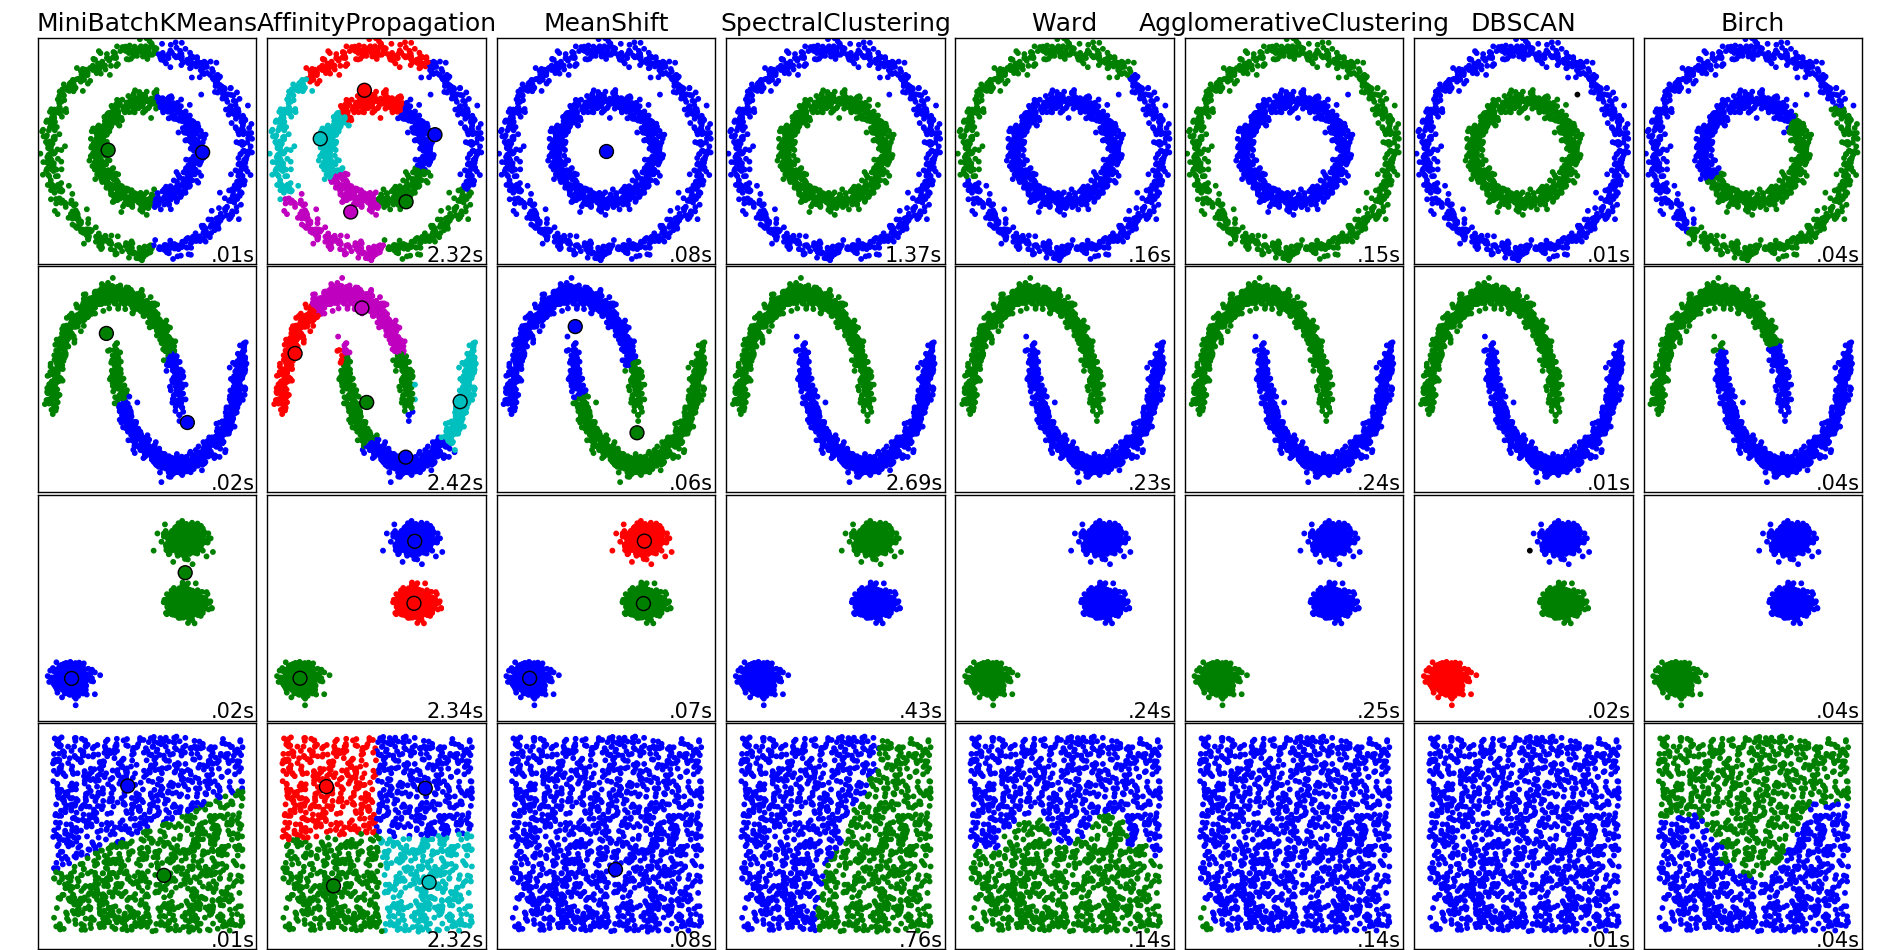
\includegraphics[width = 12cm,height = 7cm]{image/111.png}
% \caption{Comparing different clustering Algorithms }
% \label{dataclu}
% \end{figure}

Data streaming involves two main issues. First, how to process the data quickly.
Secondly, how to deal with the changes over the time.




%------------------------------------------------------------

%%---------------GHALAT ELMI-----------------------------------------------
% Streams consist of data tuples that need to be processed as they arrive, and mining these streams is challenging since the data distribution underlying
% a stream can evolve significantly over time. Besides dealing with evolving distributions, stream clustering algorithms have to meet several technical requirements, including limited time, limited memory, and processing the stream in a single pass. A multitude of stream clustering algorithms has been proposed in the literature that satisfy these requirements. 

% Of major importance is the quality of the resulting clustering, which can be measured by evaluation measures, also termed criteria, indices, validation measures, or validation indices.

%%-----------------------------------------------------------




\section{Research Objectives}

The overall research goal is to evaluate data stream clustering platform capable of generating micro and macro clusters for indoor localization data. To evaluate the proposed model, The DSAP algorithm is compared with streaming k-means data stream clustering.

The measurable objectives can be described as follows. 

\begin{itemize}
    %\item The proposed method is based on unsupervised learning, and data clustering. Affinity Propagation (AP) is a clustering message passing algorithm proposed by Frey and Dueck. This algorithm is selected for its properties of stability and of the way it represented each data cluster. The consequence of using AP is quadratic computational complexity, especially on large scale datasets.
    \item Develop the data stream AP model for uncovering evolutionary patterns with two-stage, online and offline phases.
     \item Applying landmark time window model to find the latest data point in the stream.
   
    % \item Apply the online-offline phases of such a model to analysing indoor positioning stream data.  
    % \item Applying two data related to indoor localization positioning 
    \item Analyze the behavioral pattern in indoor localization experiments.
    %has certainly not been applied 
    \item demonstrate the potential of analysing people counting data to understand staircase behavioural changes in indoor spaces before, during, and after a health motivated intervention.
    \item Apply streaming K-means clustering framework to compare the proposed model and evaluate our model.
    \item Evaluate the clustering results to find the accuracy of the proposed algorithm.




\end{itemize}
 

\section{Research Questions}


The research questions of this research work are: 
\begin{itemize}
    \item Is streaming AP more suitable than streaming K-means for analysing e-counter data? 
    \item Maintain a continuously consistent good clustering of the sequence observed so far, using a small amount of memory and time.

\end{itemize}


\section{Scientific Contributions}


The main scientific contribution of this research work summarized as follow:

\begin{itemize}
    \item A novel data stream clustering for uncovering evolutionary patterns using landmark time window model is proposed. 
    \item proposing implementations that can achieve similar quality to  Streaming K-means clustering while retaining levels of memory usage and runtime that are acceptable in a streaming environment.
    \item AP streaming clustering algorithms have certainly not been applied to analysing people counting data before.
    %elmi
    \item  providing a partitional clustering technique that can adapt to appearing or disappearing concepts in underlying data, thus achieving similar or better quality and performance of clustering than less-flexible techniques without requiring a specific level of clustering to use
    \item We demonstrate the potential of analysing people counting data to understand staircase behavioural changes in indoor spaces before, during, and after a health motivated intervention.
\end{itemize}


\todo[inline]{}research premises 
As far as we had research, there is not any research work present with affinity propagation used landmark time window model.


\section{Organization of this Thesis}
This thesis is organized in five chapters as described as follows:
Chapter 2 provides a background of clustering algorithms and stream clustering method. 

Chapter 3 summarizes the related literature and impacts for the decisions in terms of algorithms.

Chapter 4 describes the methodology including our stream clustering process and the proposed DSAP algorithm for data stream clustering.

Chapter 5 includes a summary of implementation and the applications applied for our model.

Chapter 6 provides an in-depth analysis of the data applied and the accuracy of the proposed approach and compare this model with the existing streaming k-means model.

Chapter 7 outlines the conclusion and future work research work.
% \end{document}



%Indoor positioning and occupancy models are an emerging area of interest. An exponential growth in the usage of indoor non-intrusive sensors and data interpretation algorithms has been reported in the last few years. The DSAP algorithm is proposed as a robust and efficient method to analyze indoor positioning and building occupancy datasets. MOVE THIS PARAGRAPH TO THE INTRODUCTION



%Many real-world applications require the knowledge of the user location in order to provide relevant services. Hence, many research efforts are being made to develop automatic user localization tools. The studies conducted in this work are another step in the direction. The user's position and attributes are estimating by using measurements from electronic devices or sensors. MOVE THIS PARAGRAPH TO THE INTRODUCTION


%There are challenges to designing a data stream platform, such as unbounded data or no control over the data arrival.

%%%%%%%%%%%%%%%%%%%%%%%%%%%%%%%%%%%%%%%
% Although AP still does not guarantee global optimum, several experiments in [13] have shown its consistent superiority over the previous algorithms. However, AP clustering has a limitation that it is hard to determine the value of parameter ‘preference’, which can lead to a suboptimal clustering solution.
%%----------Chapter 2------------------------------------------
% \documentclass[../UNBThesis2.tex]{subfiles}
\setlength{\parindent}{2em}
% \begin{document}
\chapter{Background}

%As the number of connected devices and applications that generate huge amount of data at very high speed increases, the need for faster data mining techniques is enhanced. This research work proposes a data stream clustering algorithm that builds upon the Affinity Propagation clustering algorithm. The concept of time windows that partition the data into manageable chunks is introduced in order to apply these algorithms for data stream clustering.

This Chapter presents an overview of clustering methods by reviewing the various concepts, methods, and underlying steps, with a particular focus on the affinity propagation (AP) method. Data stream clustering algorithms are also introduced with the time window models that are used for computing stream clusters. 

%Finally, indoor localization systems are described due to the potential wide range of services they can provide by leveraging Internet of Things (IoT) and ubiquitous connectivity. 


%K-means algorithm based clustering techniques are introduced to compare with the proposed model to evaluate it's performance. Real world indoor localization data that is discussed later in the chapter is used to test the model. 


\section{Cluster Analysis}

\subsection{Overview}
Clustering refers to partitioning a set of data points (also referred to as observations or tuples) into groups according to a proximity measure. Distance functions are predominantly used to determine a proximity measure of dissimilarity/similarity between clusters.  This proximity measure directly affects the formation of the resulting clusters. Almost all clustering algorithms are explicitly or implicitly connected to some definition of distance function \cite{zumel2014practical}. The most commonly used distance functions for quantitative feature spaces are summarized in Table \ref{tabdis}. 





\begin{table}[!ht]
\caption{Main distance functions used for computing proximity measures}
\label{tabdis}
\begin{tabular}{lll}
\hline
\multicolumn{1}{c}{\textbf{Distance}} & \multicolumn{1}{c}{\textbf{Function}}                         & \multicolumn{1}{c}{\textbf{Description}}                                                                                                                                                                                           \\ \hline\midrule
Euclidean distance                    & $\sqrt {\sum _{i=1}^{n}  \left( q_{i}-p_{i}\right)^2 }$       & \begin{tabular}[c]{@{}l@{}}The root square differences \\ between co-ordinates of a\\  pair of data points, most\\  applied way of representing\\  distance in clustering. Tend\\ to form hyperspherical \\ clusters.\end{tabular} \\ \hline
Manhattan distance                    & $ \sum_{i=1}^n \abs{q_i - p_i}$                               & \begin{tabular}[c]{@{}l@{}}The sum of the distances in \\ each dimension in a\\ n-dimensional space\end{tabular}                                                                                                                   \\ \hline
Minkowski distance                    & $\left( \sum_{i=1}^n \abs{q_i - p_i}^n \right)^{\frac{1}{n}}$ & \begin{tabular}[c]{@{}l@{}}The generalization of the\\  Euclidean distance and \\ the Manhattan distance\end{tabular}                                                                                                              \\ \hline
Cosine distance                       & $1 - cos \alpha = \frac{q_i^{T} - p_i}{\|q_i\| \|p_i\|}$      & \begin{tabular}[c]{@{}l@{}}A metric for measuring \\ distance when the \\ magnitude of the vectors\\  does not matter, commonly\\  used in text data\end{tabular}                                                                  \\ \hline
Mahalanobis distance                  & $\sqrt{(q_i - p_i)^T S^{-1} (q_i - p_i)}$                     & \begin{tabular}[c]{@{}l@{}}The distance between a data\\  point and the mean, requiring\\  high computational complexity\end{tabular}                                                                                              \\ \hline\midrule
\end{tabular}
\end{table}






Figure \ref{clus} illustrates the results of a clustering process for a set of points in a 2D space, where different data points were partitioned into three clusters using the Euclidean distance. Each cluster is represented by its centroid or exemplar (red data points). In general, the intra-cluster data points are similar due to their proximity in the feature space, meanwhile the inter-cluster data points are dissimilar. 

\begin{figure}[!ht]
    \centering
    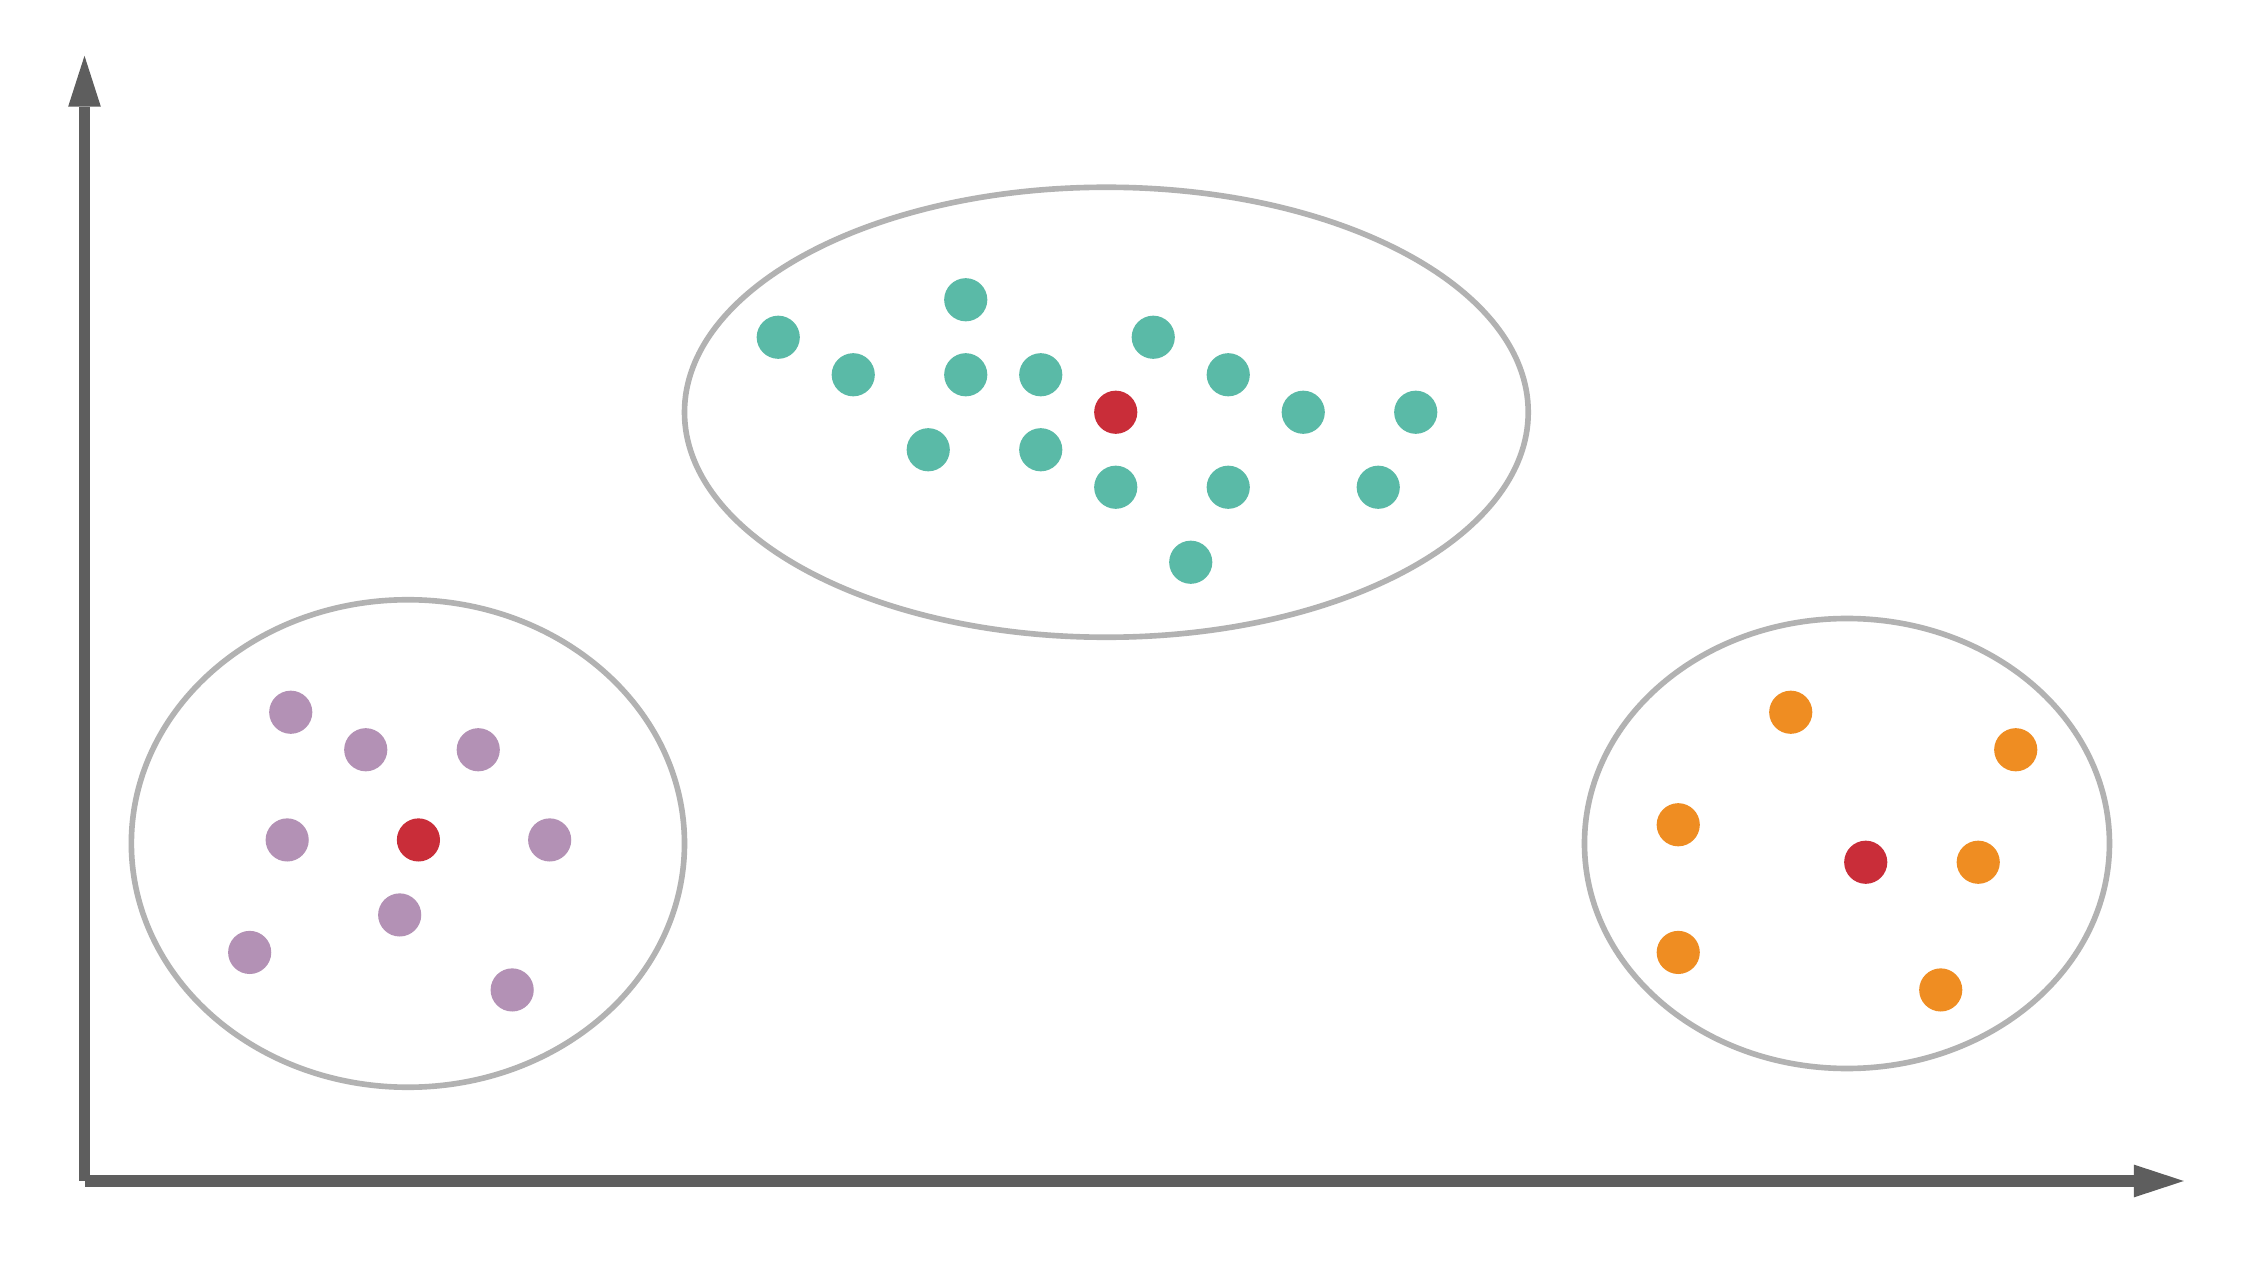
\includegraphics[width = 8 cm]{image/Chapters/Chapter2/Blank diagram (1).png}
    \caption{Clustering in 2D feature space}
    \label{clus}
\end{figure}


Once a proximity measure is chosen, the construction of a clustering criterion function makes the partition of
clusters an optimization problem, which is well defined
mathematically, and has rich applications in marketing, biomedical and geospatial fields \cite{jain1999data}. 

\subsection{Clustering Methods}

Clustering is ubiquitous, and a wealth of clustering methods has been developed to solve different problems in specific fields. However, there is no clustering method that can be universally used to solve all problems. Some problem examples can be described as follows: 

\begin{itemize}
    \item \textit{Group Discovery}: Clusters provide useful information for supporting a pre-processing step of discriminant analysis. 
    \item \textit{Pattern Recognition}: Clusters can be used for supporting template matching by determining similarities between two entities of the same type (e.g., points, curves, or shapes), finding patterns and regularities in data.
    
   % the information stored in the database with the incoming data. 
    \item \textit{Data Compression}: Clusters provide a summary of a data set by reducing the number of data points needed to represent a data set. This is achieved by using cluster centroids rather than the actual data points. 
    
   % its most representative object which can be a center of mass or an actual data point as a centroid.
    \item \textit{Outlier detection}: Clustering has been successfully applied to find outliers in data. % is another method in which many applications employ anomaly detection, such as intrusion detection, fraud detection. Anomaly detection is achieved by identifying outliers. 
    An outlier can be assigned to a data point very far from its cluster centroid or a cluster that deviates from the prominent clusters.
    \item \textit{Feature Reduction}: Clusters can be used for dimension reduction when the number of features in a data set is larger than the number of data points.
    \end{itemize}




%Even though labeled data can be analyzed using clustering techniques, but the strength of this unsupervised approach (or exploratory learning) lies in detecting similarities within an unlabelled dataset. 



% and these two words bring distances of each data point in the cluster which is closer to other data points than other data points in other clusters \cite{zumel2014practical}. 


% The Euclidean distance is the most common one, and this is what we applied in our work. It calculated the root of square differences between two pairs of data points.
% Manhattan distance which computes the absolute differences between two data points.
% Minkowski distance is ---
% Cosine distance is a common similarity metric in text analysis. It measures the smallest
% angle between two vectors \cite{zumel2014practical}.
% Mahalanobis distance---
% Categorical data usually applies Hamming distance which a number of attributes taking different values \cite{han2001data}.




Therefore, selecting a clustering method is an important step, as certain methods might be best-suited for a particular type of data sets in order to reflect the true nature of the data \cite{berkhin2006survey, han2011data}. Traditionally, clustering methods can be distinguished into five main categories described as follows: 

%The advantages and disadvantages of all these methods are listed next in \ref{methoda}.
%In progress

\begin{itemize}

    \item\textit{Partitioning methods:} In these methods data points are split into $k$ number of clusters. Each data point can only belong to one cluster, and each cluster must contain at least one data point. The algorithms usually require a distance threshold %the distance of new data points to the existing micro-clusters, and maybe it comes(happen) 
    to generate new clusters, specially those with spherical shapes.   %. These types of algorithms are 
    %finding clusters with spherical shapes. %, and the noise can influence the results. A very famous algorithm in this group is K-means.
    K-means is the most recognized clustering algorithm in this category due to its robustness in finding clusters that have not been explicitly labeled in the data.
    
    \item\textit{Hierarchical methods:} The aim is to build a tree-like nested structure from a set of data points \cite{swarndeep2016overview}. Initially each data point is considered as an individual cluster, and at each iteration, a proximity matrix is computed to merge similar clusters until one cluster or $k$ clusters are formed. These methods are widely used to analyze social network data. The BIRCH algorithm is an example of a hierarchical method where every data point is equally important for clustering purposes. Moreover, the concept of Clustering Feature (CF) is fundamental for summarizing the information that needs to be maintained about a cluster.
    
    %The clusters are described in the form of dendrogram. %It can be analyzed with the help of statistical method. 
    
    %the algorithm related to this group.
    %elmi
    \item\textit{Density-based methods:} Clusters are separated from each other by contiguous regions of low density of data points. They are highly efficient to find arbitrary shaped clusters and clusters with noise.  DBSCAN and OPTICS are well-known algorithms in this group.
    
    %continue to grow the given cluster as long as the density in the neighborhood. 
    
% exceeds certain threshold
    %elmi
    \item\textit{Grid-based methods:} %are a special category of density-based algorithms, where the regions consists of the grid cells. In particular, 
    The feature space is partitioned into a finite number of cells to form a grid structure and then find the clusters from the cells. These methods are efficient in mining large multidimensional data sets. STING is one of the highly scalable algorithms in this group with the ability to decompose a feature space into various levels of detail. 
   
    %elmi
    \item\textit{Model-based methods:} The main assumption is that the data points are generated by a model which can be adapted to what we know about the underlying distribution of the data. The model that we recover from the data then defines clusters and an assignment of data points to new clusters. A commonly used criterion for estimating the model parameters is maximum likelihood.
    
    %try to fit a model to the data, assuming that data are generated from k probability distributions (typically Gaussian).
\end{itemize}

The main advantages and disadvantages of these different clustering methods are summarized in Table \ref{methoda1}. 

\begin{table}[!ht]\scriptsize
% \centering
\caption{ Comparison of clustering methods}% \protect\cite{mousavi2015data}
\label{methoda1}  
\small
\begin{tabularx}{\linewidth}{p{3cm} p{5.5cm} p{5.5cm}}
\hline
 \multicolumn{1}{c}{\textit{\textbf{Categories}}} &
 \multicolumn{1}{c}{\textit{\textbf{Advantages}}}   &   
\multicolumn{1}{c}{\textit{\textbf{Disadvantages}}} 
\tabularnewline \hline
\vfill 
 \textbf{Partitioning Methods}    & 
 \begin{enumerate}[*,topsep=0pt,leftmargin=0.2cm]
 \item Easy to implement  
 \item Produce tighter clusters
\end{enumerate}
\tabitem
&       
\begin{itemize}[*,nosep,leftmargin=0.2cm]
    \setlength\itemsep{0em}
     %\item Require pre-defined value for number of clusters  THIS IS NOT CORRECT, SINCE AP DOES NOT REQUIRE THE NUMBER OF CLUSTERS
     \item Best suited for finding spherical shaped clusters
\end{itemize} 
\tabularnewline \hline

\vfill
\textbf{Hierarchical Methods}
& 
\begin{itemize}[*,nosep,leftmargin=0.2cm]
    \item Easy to handle any type of distance function   
\end{itemize}
 &       
\begin{itemize}[*,nosep,leftmargin=0.2cm]
  % \item High ambiguity of clustering criteria 
    \item High computational complexity
\end{itemize}
\tabularnewline \hline
\vfill
\textbf{Grid-based Methods}
& 
\begin{itemize}[*,nosep,leftmargin=0.2cm]
    \item Fast processing time 
    \item Effective with handling noisy data
\end{itemize}
&      

\begin{itemize}[*,nosep,leftmargin=0.2cm]
    %\item Higher value for convex clusters
    \item Limited to the Euclidean distance function
\end{itemize}
\tabularnewline \hline
\vfill
 \textbf{Density-Based Methods}
& 
\begin{itemize}[*,nosep,leftmargin=0.2cm]
    \item Fast to compute
    \item Easy to interpret clusters %as it gives higher value when clusters are dense
\end{itemize}
 &       
\begin{itemize}[*,nosep,leftmargin=0.2cm]
    \item Higher value for convex clusters compared with density-based clusters
\end{itemize}
\tabularnewline \hline
\vfill
 \textbf{Model-Based Methods}
& 
\begin{itemize}[*,nosep,leftmargin=0.2cm]
    \item Offer more flexibility
    %Number of clusters based on standard statistics 
    \item Effective in handling noisy data            
\end{itemize}
 &       
\begin{itemize}[*,nosep,leftmargin=0.2cm]
    \item Highly dependent on the hypothesized model
\end{itemize} 
\tabularnewline \hline
\vfill
\end{tabularx}
\end{table}



% \begin{table}[htbp]
% \caption{Comparison of clustering methods}
% \label{methoda1}
% \begin{tabular}{
% >{\columncolor[HTML]{FFFFFF}}l ll}
% \hline
% \multicolumn{1}{c}{\cellcolor[HTML]{FFFFFF}\textit{\textbf{Categories}}}  & \multicolumn{1}{c}{\cellcolor[HTML]{FFFFFF}\textit{\textbf{Advantages}}}                               & \multicolumn{1}{c}{\cellcolor[HTML]{FFFFFF}\textit{\textbf{Disadvantages}}}                                          \\ \hline
% \textbf{\begin{tabular}[c]{@{}l@{}}Partitioning \\ Methods\end{tabular}}  & \begin{tabular}[c]{@{}l@{}}*Easy to implement\\ *Produce tighter clusters\end{tabular}                 & \begin{tabular}[c]{@{}l@{}}*Best suited for finding spherical \\ shaped clusters\end{tabular}                        \\ \hline
% \textbf{\begin{tabular}[c]{@{}l@{}}Hierarchical \\ Methods\end{tabular}}  & \begin{tabular}[c]{@{}l@{}}*Easy to handle any type \\ of distance function\end{tabular}               & *High computational complexity                                                                                       \\ \hline
% \textbf{\begin{tabular}[c]{@{}l@{}}Grid-based\\  Methods\end{tabular}}    & \begin{tabular}[c]{@{}l@{}}*Fast processing time\\ *Effective with handling \\ noisy data\end{tabular} & \begin{tabular}[c]{@{}l@{}}*Limited to the Euclidean \\ distance function\end{tabular}                               \\ \hline
% \textbf{\begin{tabular}[c]{@{}l@{}}Density-Based\\  Methods\end{tabular}} & \begin{tabular}[c]{@{}l@{}}*Fast to compute\\ *Easy to interpret clusters\end{tabular}                 & \begin{tabular}[c]{@{}l@{}}*Higher value for convex \\ clusters compared with \\ density-based clusters\end{tabular} \\ \hline
% \textbf{\begin{tabular}[c]{@{}l@{}}Model-Based\\  Methods\end{tabular}}   & \begin{tabular}[c]{@{}l@{}}*Offer more flexibility\\ *Effective in handling noisy\\  data\end{tabular} & \begin{tabular}[c]{@{}l@{}}*Highly dependent on the\\  hypothesized model\end{tabular}                               \\ \hline
% \end{tabular}
% \end{table}





\subsection{Affinity Propagation Clustering}

% $O(N^2logN)$ where N is the number of data points. It can be imagined that if the number of data points is very huge, then it is impossible to do clustering using AP
Affinity propagation (AP) is a partitioning-based clustering algorithm that was first introduced by Frey and Dueck in 2006 \cite{frey2006mixture}. AP is based on the concept of "message passing" between data points that plays an important role in finding the best candidate data point that becomes a cluster centroid \cite{frey2007clustering, jiang2019exemplar}. 



%It means to find data points with the maximum similarity to others. The advantage of AP to compare with many clustering algorithms is that this Algorithm does not require the number of clusters as an input, and it makes it unique between many clustering algorithms.


Unlike clustering algorithms such as k-means, affinity propagation does not require the number of clusters to be determined or estimated before running the algorithm. It considers all data points as a potential centroids until an optimal set of clusters and their respective centroids are found through an iterative process. %as illustrated in Figure \ref{APPi}. 
% \todo[inline]{Please explain the contents of this figure}

%illustrates the gradually emerging of clusters and centroids, but the tenth iterations show the uncertainly of having clusters shows with the faded blue lines until the last and final iteration to find a good cluster solution. NOT POSSIBLE TO UNDERSTAND THE MESSAGE OF THIS PARAGRAPH

% \begin{figure}
% \centering
% 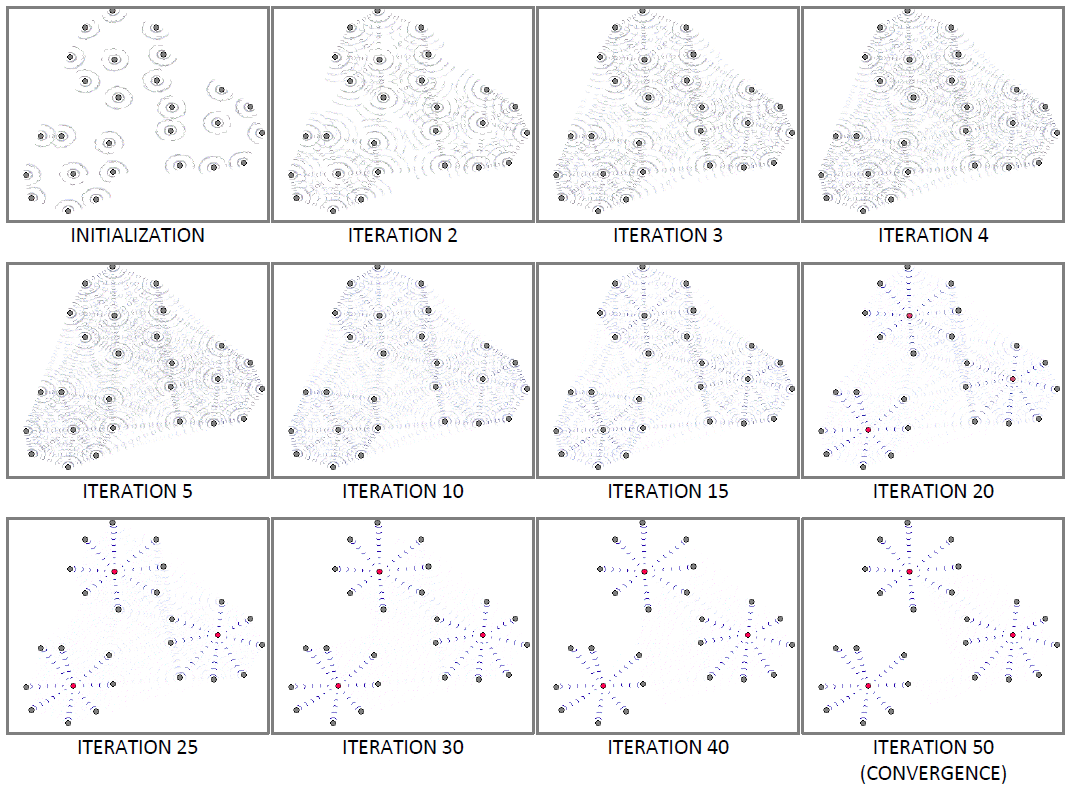
\includegraphics[width = 13 cm]{image/Chapters/Chapter2/APDurek.PNG}
% \caption{Iteration process of affinity propagation (Source: \protect\cite{dueck2009affinity})}
% \label{APPi}
% \end{figure}


The AP algorithm supports similarities that are not symmetric, and it is not dependent on initialization found in other clustering algorithms \cite{refianti2017time}. In order to apply AP for any data set two conditions should be met: no missing or null data in the inputs and the feature space should contain only numeric, not categorical data. However, it has a significant speed problem, particularly for clustering large volume of data. Affinity Propagation needs $O(N^2T)$ time to update a message where $N$ and $T$ represent the number of data points and the number of iterations \cite{frey2007clustering}. 


The AP algorithm is based on the computation of four matrices: similarity matrix, responsibility matrix, availability matrix, and criterion matrix. They are described as follows:

\begin{itemize}

  \item\textit{Similarity Matrix:}
  Every cell value in the similarity matrix $s(i,j)$ corresponds to an element \textit{k} representing how similar/dissimilar two data points are in a feature space. This element \textit{k} is defined as the negative of the Euclidean distance between the two data points. 
  
  \begin{equation}
      s (i,j) = - \norm{x_i - x_j}^ 2
  \end{equation}
  
  The greater the distance between any two data points, smaller is the \textit{k} between them. The \textit{k} values of the off-diagonal cells will dictate the number of clusters formed, in such a way that the smaller the index value (value	$\leq$0), fewer number of clusters is obtained.
  %gives information about any inputs. It shows data points with is how appropriate to be the cluster-head for data point \textit{i}. 
  %Every cell has values that correspond to how similar two objects are. It is a diffident method to calculate the values for diagonal values and non-diagonal values.  The diagonal values,  Cells are filled with the lowest number among all the cells. The non-diagonal values are the negation of the sum of the squares of the differences between participants.
  \item\textit{Responsibility Matrix:} The matrix $r(i , k)$ quantifies how well-suited element $k$ is, to be a cluster centroid for element $i$, taking into account the nearest contender $k^{\prime}$ to be a cluster centroid for $i$.
  
  %Cells contain values that correspond to how responsible one data point is for another. It is better to say how responsible it is to be a part of another object or related to another object. 
  We initialize the matrix $R$ with zeros, and compute the next values using the equation:

    \begin{equation}
        r(i, k) \leftarrow s(i, k) - \max\limits_{k' s.t. k' \neq k}\{ a(i, k') + s(i, k') \}
    \end{equation}
 
 The goal is to quantify how similar is $i$ to $k$, compared to some $k^{\prime}$, taking into account the availability of $k^{\prime}$.   
    
  \item\textit{Availability matrix:} The matrix $a(i,k)$ quantifies how appropriate is it for $i$ to choose $k$ as its cluster centroid, taking into account the support from other elements that $k$ should a centroid. Availability is self-responsibility of $k$ plus the positive responsibilities of $k$ towards elements other than $i$ as shown in the following equation:
  
    \begin{equation}
        a(k, k) \leftarrow \sum\limits_{i' \neq k}\max(0, r(i', k))
    \end{equation}
  
  The matrices $R$ and $A$ matrices are iteratively updated. This procedure may be terminated after a fixed number of iterations, after changes in the values obtained fall below a threshold, or after the values stay constant for some number of iterations.
  
  
%   \begin{equation}
%         (i, k) \leftarrow \min\{0, r(k,k) + \sum\limits_{i' s.t. i' \notin \{i, k\}}{\max\{0, r(i', k)\}}
%     \end{equation} 
  
 % This matrix contains values that correspond to how available one object is to be a centroid for another object. With this means, how available one object is for a cluster to be a centroid of a cluster, and diagonal values is the sum of all positive responsibility values in the column excluding the object self-responsibility. 
 % The availability diagonal values are determined by the following formulas:

  Figure \ref{abc} illustrates how the AP algorithm sends responsibility and availability messages to data points \protect\cite{dueck2009affinity}. Responsibility $r(i,k)$ is the message from data point $i$ to candidate centroid $k$ and answer relies on determining if point $k$ is well-suited to be a centroid for data point $i$. Availability $a(i,k)$ sends a message from centroid $k$ to data point $i$ to find how well it would be for point $i$ to choose point $k$ as a centroid. 
    


    \begin{figure}
    \centering
    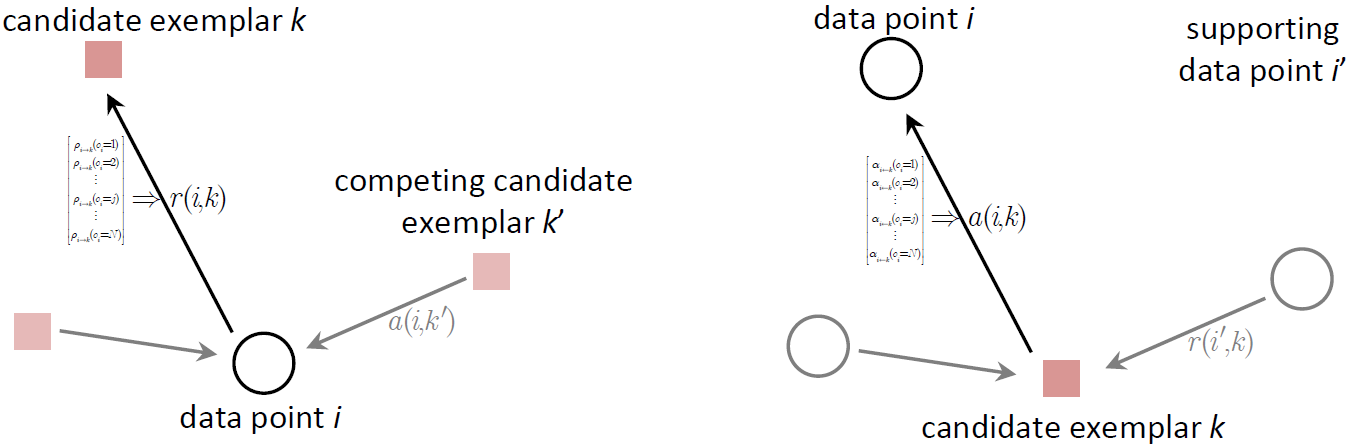
\includegraphics[width = 13 cm]{image/Chapters/Chapter2/APmessage.PNG}
    \caption{Message passing based on responsibility and availability matrices}
    %AP sends two types of message towards other data points: responsibility and availability \protect\cite{dueck2009affinity}. Responsibility $r(i,k)$, is the message from data $i$ to candidate centroid $k$ and the respond back to figure out if point $k$ is well suited as a centroid for point $i$.    Availability $a(i,k)$, send a message from centroid $k$ to point $i$ to find how well it would be for point $i$ to choose point $k$ as a centroid. ##########THIS IS TOO MUCH TEXT TO BE PART OF A FIGURE CAPTION###########}
    \label{abc}
    \end{figure}


  \item\textit{Criterion matrix:} This matrix is calculated after the iteration process is terminated.The $c (i,k)$ matrix is the sum of $R$ and $A$. An element $i$ will be assigned to an exemplar $k$ which is not only highly responsible but also highly available to $i$  as shown in 
    
    \begin{equation}
        c(i, k) \leftarrow r(i, k) + a(i, k)
    \end{equation}
    
  %\todo[inline]{put the equation for the C matrix here}
  
  %Lastly, in the criterion matrix, each cell is the sum of the availability matrix and responsibility matrix. The highest criterion values of each row are designated as a centroid.

The element with the highest criterion value in each row would be designated to be a cluster centroid. Elements that have the same centroid will be in the same cluster.







\end{itemize}

The AP clustering algorithm used in this thesis is described in Algorithm \ref{APo}. The Python code used in this work is available at https://scikit-learn.org/ open source repository. Four hyperparameters are used for tuning the clustering process using AP. They are described as follows: 

\begin{itemize}

\item Damping Factor is the extent to which the current value is maintained relative to incoming values (weighted 1 - damping). This is used to avoid numerical oscillations when updating messages. The range of this hyperparameter is between 0.5 to 1.

\item Maximum number of iterations.

\item Convergence is the number of iterations with no change in the number of estimated clusters that stops the convergence.

\item Preference values indicates how likely a point is to be an exemplar. If the preferences are not passed as arguments, they will be set to the median of the input similarities.
%Preference is the number of centroids influenced by the input preferences value.
% \item Affinity is the selection of which distance function to use.


    % \item\textit{Preference Parameter:} determines a p how likely is a data point $i$ to be chosen as a centroid. This value is in the diagonal of similarity matrix. The number of identified clusters can be increased or decreased by changing this parameter correspondingly, and a good choice is to set the preference to be the median of all the similarities between data points \cite{li2012improved}.
    % %This value for the e-counter dataset for the online phase is -4 and the value of the offline phase is -1. This number is a median value of the similarity matrix.
    % \item\textit{Damping factor:}  is the extent to which the current data point is maintained relative to incoming data points. Damping should be between 0.5 to 1. 
    % \item\textit{Maximum number of iteration:}  defines the maximum number of iterations. The default value for both online and offline phase is 100.
    % \item\textit{Convergence iteration:}  is the number of iterations with no change in the number of estimated clusters that stop the convergence.
\end{itemize}

\begin{algorithm}[htbp]
 \caption{Affinity Propagation Algorithm}
\label{APo}
    \SetKwInOut{Input}{Input}
    \textbf{Input:} Data $d=(d_{1}, d_{2},...,d_{n})$\\
    \textbf{Hyper-parameters:}
        {Preference, Damping,  $conv_{it}$, $max_{iter}$}\\
\textbf{Output:} {Cluster centroids $C_1, ..., C_k$, branch points }\\
  	\SetKwFunction{FIROC}{AP}
    \SetKwProg{Fn}{Function}{:}
    \Fn{\FIROC{$d$}}{
        \textbf{Initialization:}\\
        {Similarity Matrix: S $\forall$ i, k:  s(i, k)} = 0\newline
        {Availability Matrix: A $\forall$ i, k:  a(i, k)} = 0\newline
        {Responsibility Matrix: R $\forall$ i, k:  r(i, k)} = 0\newline
        {Criterion Matrix: E $\forall$ i, k:  e(i, k)} = 0\newline
     \textbf{Compute S:}
        {$\forall i, k:  s(i, k) \leftarrow -\norm{V_i - V_k}^2 where V_i = (M_i, S_i) $}\newline
  	 \emph{
  	 \While{$r(i,k)\ \&\ a(i,k) \neq $convergence}{
  	 \textbf{Compute R:}\newline
  	       $r(i, k) \leftarrow s(i, k) - \max\limits_{k' s.t. k' \neq k}\{ a(i, k') + s(i, k')$ \}\newline
  	       \textbf{Compute A:}\newline
  	       $a(i, k) \leftarrow \min\{0, r(k,k) + \sum\limits_{i' s.t. i' \notin \{i, k\}}{\max\{0, r(i',k) \}}$\newline
  	       \textbf{no-diagonal A:}\newline
  	       $a(i, k) \leftarrow \sum\limits_{i' \neq k}\max(0, r(i', k))$\\
  	       \textbf{cluster assignment: $E = (E_1,..E_n)$ $E = argmax[a(i,k) + r(i,k)]$}
  	       }
  	       }
  	       
          	  }  \textbf{Results }C = $(C_1, ..., C_k)$

\end{algorithm}





%To improve the algorithm performance, hyper-parameters should be considered. These parameters are variables that control the performance and structure of any machine learning model and they are grouped in four, Preference, damping maximum iteration, and convergence iteration. These parameters are described below.

%elmi-In un-convergent cases, we have to increase lam manually and gradually and rerun AP until the algorithm converges. Another choice is to use a big damping factor close to 1 to eliminate oscillations, but AP will run very slow. Both choices may consume plenty of time, especially for a large data set
%    \item Number of initial data points: 500 items from the head of the stream
 %   \item Threshold($\epsilon$): This number is the average distance between data points and exemplars in the first phase. For e-counter dataset it is equal to 1.

%) preferences for each data point that is more likely to be chosen as an exemplar. 2) $convergence\_iter$ is the number of iterations with no change in the number of estimated clusters that stop the convergence. 3) damping factor (between 0.5 and 1) is the extent to which the current data point is maintained relative to incoming data points (weighted 1 = damping); and 4) $max\_iter$ defines the maximum number of iterations.







% \subsection{K-means Clustering} \label{kmeansalgo}
% \todo[inline]{Nasrin you need to improve this section}

% K-means was first introduced by J.MacQueen in 1967 \citet{macqueen} as a method for partitioning numerical data into isotropic clusters.% and is not as versatile as single link algorithms. 
% It is a distance based algorithm  which aims to assign each observation to a cluster with the nearest mean (cluster centroid) based on it's distance from the centroid. The number of clusters need to be defined in advance. This is not straightforward task since no prior information is generally available.

% K-means is a suitable algorithm due to its simplicity and low computational costs. The complexity for $n$ iterations of the K-means algorithm is $O(n*K*m*N)$, where $n$ is a number of iterations, $K$ set of macro clusters, $m$ is the sample size with N attributes.  This linear complexity is one reason for the popularity of the Kmeans algorithms. It guarantees convergence and scales quite well to large datasets owing to lower memory requirements. The algorithm can be generalized to clusters of different shapes and sizes, such as elliptical clusters. Other reasons which make the algorithm so popular are a straightforward interpretation of clusters, simplicity of implementation, fast convergence, and adaptability to sparse and large data \cite{dhillon2001concept}.

% However, this algorithm is receptive to noisy data or outliers (one data point as an outlier can increase the squared error dramatically). It is suitable for data with spherical/convex clusters and well defined mean values. The output of K-Means algorithm depends on the initial value of the centroids which are the basis for the cluster determination. In essence, it is an optimization problem where a local optimal clustering can be achieved, whereas a global optimal is not always guaranteed. It is advised to run the algorithm multiple times in order to reduce the chances of a local minima solution. %It is a heuristic algorithm in which the final clustering results highly depend on the initial settings, although a reasonably good approximation is possible. 

% The main goal of K-means as a partitioning algorithm is to minimize the sum of the distances between the n data points and their representative cluster centroids into k sets $(S = s_1,...,s_n)$ and cluster them in an iterative manner. In the other words, its objective is to find:

% \begin{equation}
%     \sum_{i=1}^k \sum_{x \in S_i} \norm{x-\mu}^2
% \end{equation}

% Where $\mu$ is the mean of data points in $S_i$. However, the pre-assumption in the above equation is that the distance between the data points is the squared Euclidean distance and computed as $\norm{x - \mu}^2$. Although there are other distance metrics to find the closest distance, the Euclidean distance is widely used by other researchers owing to it's easy interpretation with low dimensional data. 

% The K-means algorithm consists of the following steps that are illustrated in Figure \ref{ite}.
% \begin{enumerate}
%     \item Randomly select k points as centroids of clusters based on the predefined value of k. These data points describe the initial set of centroids.
%     \item To create the k clusters, every data point from the dataset is assigned to the nearest centroid. The Euclidean distance is used for calculating the distance between each data point and the initial centroids. 
    
%     \item After all the data points have been assigned to their closest groups, the positions of the k centroids is recalculated by averaging all of the data points assigned in each cluster.
    
%     \item  Steps 2 and 3 are repeated until convergence is reached. This is achieved if the centroid values do not change further, the sum of distances between the data points and the centroid of each cluster does not change, the data points assigned to all clusters are the same as the previous assignment, or the maximum iteration number has been reached in case the algorithm is given a fixed iteration.
% \end{enumerate}

% \begin{figure}
% \centering
% 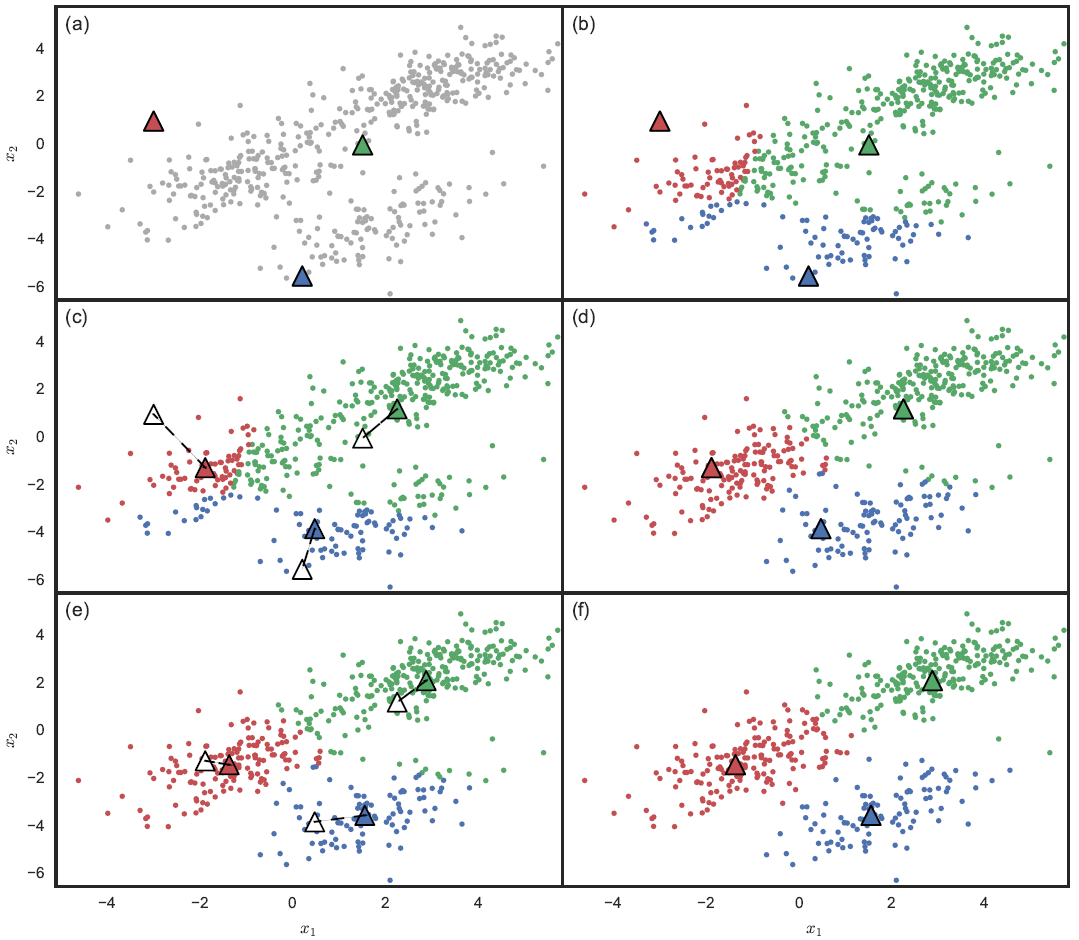
\includegraphics[width = 10 cm]{image/Chapters/Chapter2/kmeanshif.png}
% \caption{K-means Algorithm: finding clusters in a 2D data space iteratively \protect\cite{benavente2017automatic}. (a)cluster centroids initialized randomly, (b) data points map to the closest centroids, (c) centroids are moved to the mean of each cluster map points, (d,e,f) steps b and c are repeated iteratively until convergence.}
% \label{ite}
% \end{figure}

% % In the next step,  the centroids are moved to the mean of each cluster's mapped points which ${\mu_k}$ is the mean of cluster $k$ :
% % \begin{equation}
% %     {\mu_k} = \frac{1}{{N_k}}\sum_{q=1}^{{N_k}} {x_q}
% % \end{equation}

% %In this formula, $N_k$ is the number of instances belonging to cluster $k$
% % Finally, these process will be repeated until convergence. 


% % The K-means algorithm starts with the K initial set of cluster-centers and iteratively updates it to decrease the error function. A proof of the finite convergence of the K-means type algorithms is given in \cite{selim1984k}. 

% The K-means clustering algorithm that has been used in this thesis is described in Algorithm \ref{kmeanalgo}. The Python code for this algorithm as well as AP is available at https://scikit-learn.org/ open source repository. 



% \begin{algorithm}[H]
% \SetAlgoLined
% \small
% \textbf{Input:} {Data: $X$ = ${x_1,..., x_n}$}\\
% \textbf{Hyper-parameters:} {Number of clusters k, $max\_iter$}\\
% \textbf{Output:} {Set of cluster with the centroids $C = {c_1,..., c_k}$ }\\
% \textbf{Initialization:} {Set $\mu_i$, $i = 1,..., k$ to random data points }\\
% \While{(Convergence)}{
%   \For{i= 1 : n}{
%     \small\color{blue}\texttt{Assign each data point to the closest centroid:}
%     \color{black}\\
%     R_{ij} =  \arg \min_j ||x_i - \mu_j||^2, 
%     j \in 1, ..., k 
  
%   }
  
%   \For{j = 1 : k}
%   {
%     \small\color{blue}\texttt{Update each centroid by the mean value of data points within each cluster:}
%     \color{black}\\
%     n_j = \sum_{i=1}^n R_{ij}\\
%     \mu_j = \frac{1}{n_j} \sum_{i = 1}^n R_{ij} x_i
    
%   }
%  }
% {

% \textbf{return} {$\mu_1 , ... , \mu_k$\\ }
% }
%  \caption{ K-means Clustering Algorithm}
%  \label{kmeanalgo}
% \end{algorithm}

%  % \begin{equation}
% % J = \sum_{n=1}^{N} \sum_{k=1}^{K} r_{nk} ||x_n - \mu_k||^2
% % \label{eqn:kmeans_objective_function}
% % \end{equation}
 
 
 
% % Figure \ref{kmAlgo} presents the pseudo-code of K-means algorithm.

% % \begin{figure}
% % \centering
% % 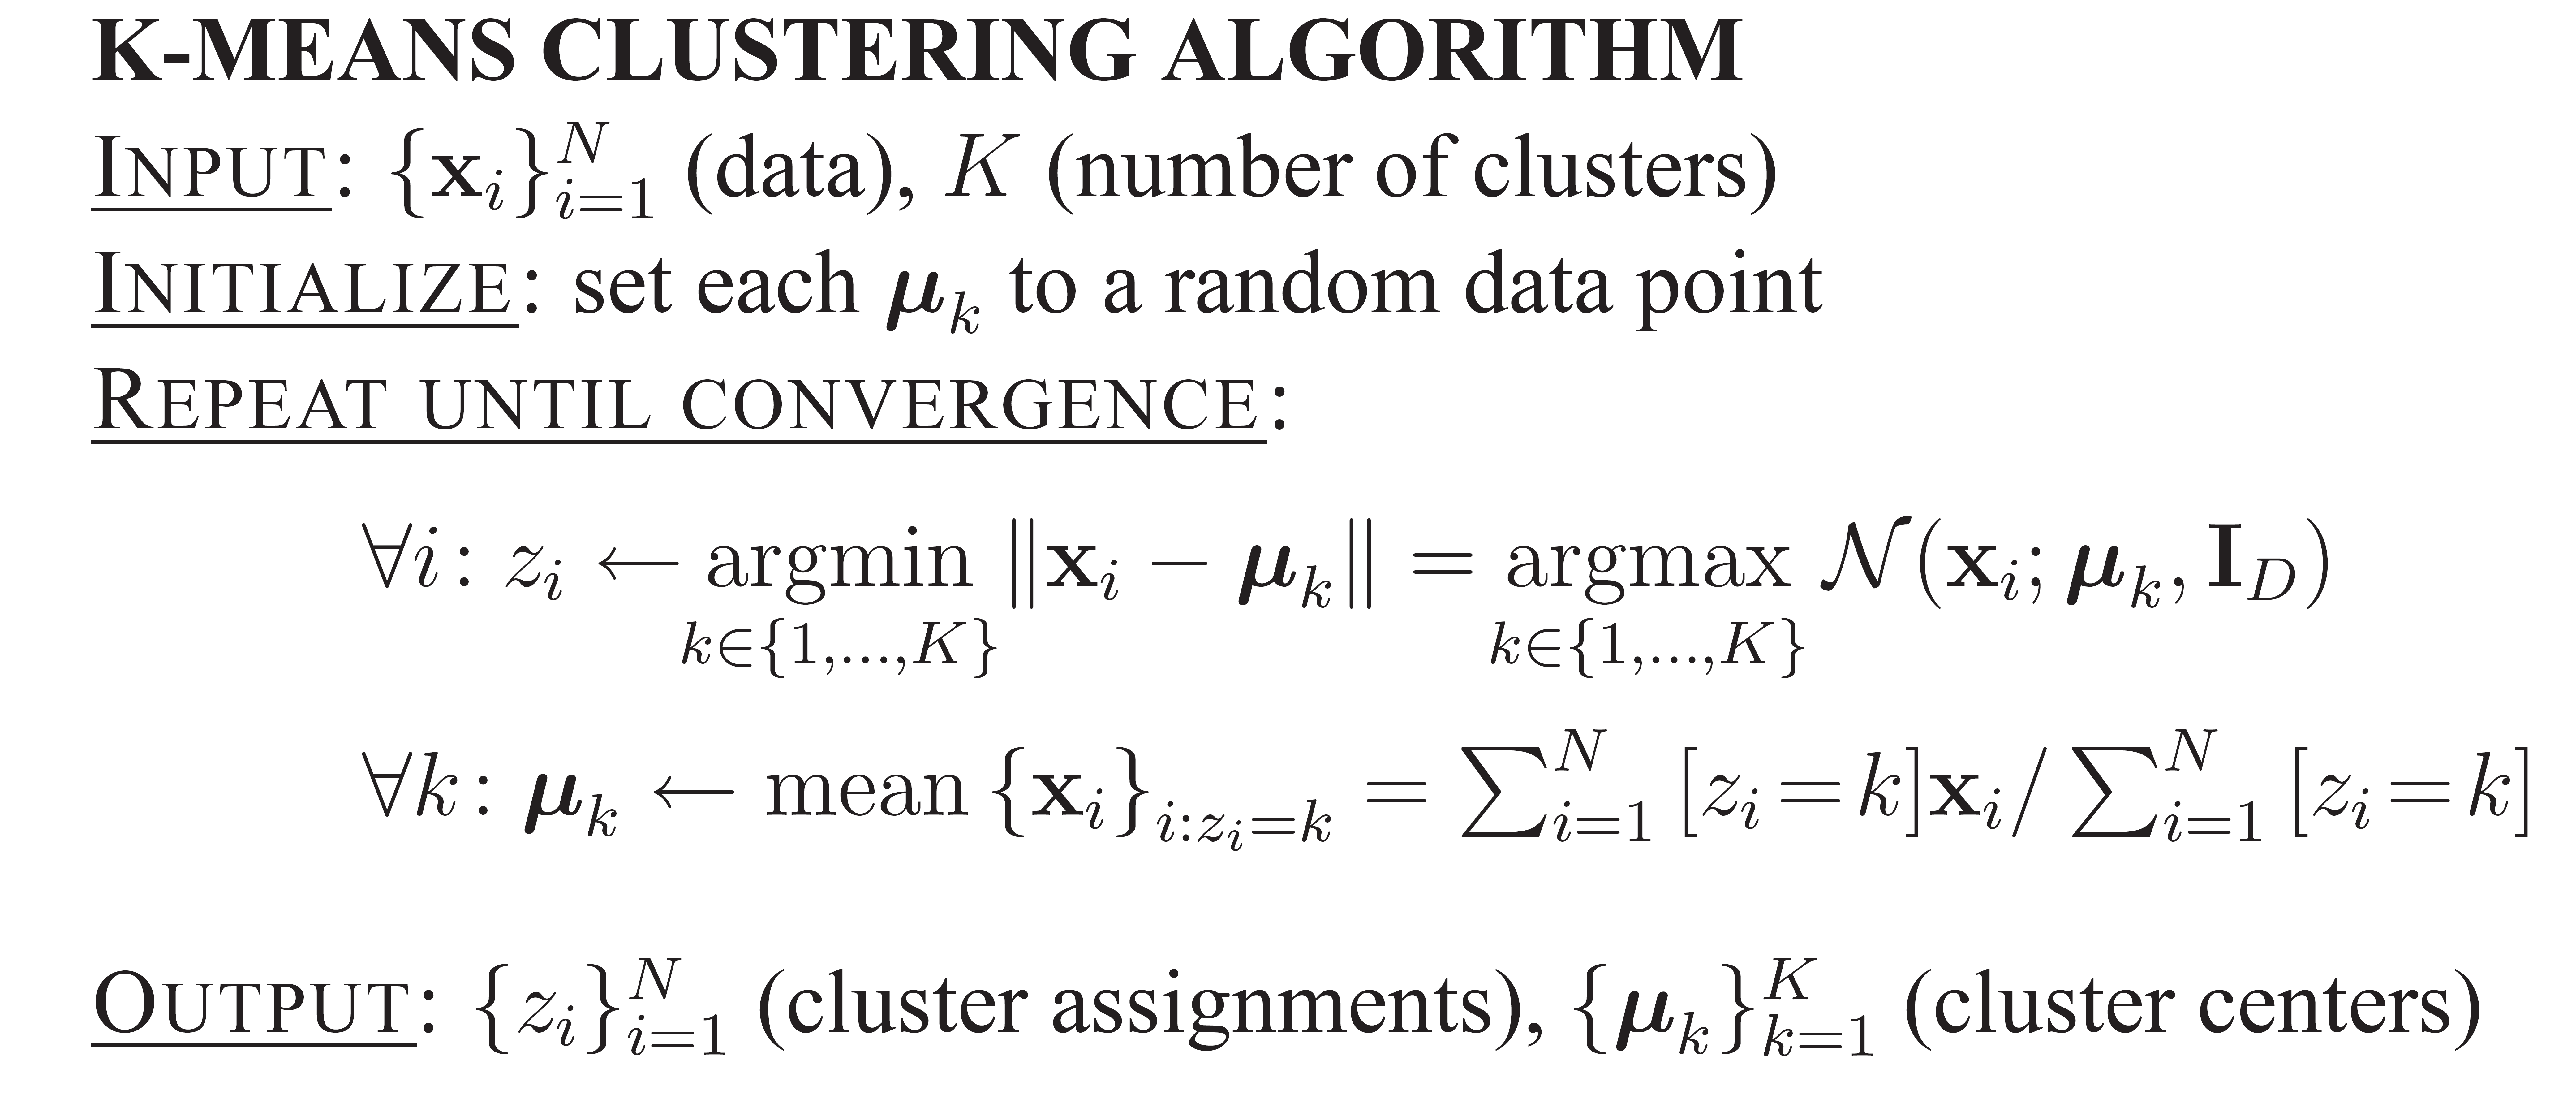
\includegraphics[width = 10cm,height = 4cm]{image/Chapters/Chapter2/6.png}
% % \caption{K-means pseudocode }
% % \label{kmAlgo}
% % \end{figure}
% \todo[inline]{make a proper for the algorithm}

% %%Elmi
% % The similarity measure on numeric attributes is the square Euclidean distance; the similarity measure on the categorical attributes is the number of mismatches between objects and the cluster prototypes.

%  %%%%%%%%%%%%%%%%%%%%%%%%%  ELMI

% % A number of convergence conditions are possible. For example, the search
% % may stop when the partitioning error is not reduced by the relocation of the centers.
% % This indicates that the present partition is locally optimal. Other stopping
% % criteria can be used also such as exceeding a pre-defined number of iterations.


% % The Achilles heel of the K-means algorithm involves the selection of the initial partition. The algorithm is very sensitive to this selection, which may make the difference between global and local minimum.
% % K-Means is one of the simplest unsupervised learning algorithms that solve the well known clustering problem. The procedure follows a simple and easy way to classify a given data set through a certain number of clusters (assume k clusters) fixed a priori.The main idea is to define k centroids, one for each cluster. These centroids should be placed in a cunning way because of different location causes different result. So, the better choice is to place them as much as possible far away from each other.The next step is to take each point belonging to a given data set and associate it to the nearest centroid. When no point is pending, the first step is completed and an early group is done. At this point, it is needed to re-calculate k new centroids as centers of the clusters resulting from the previous step. After these k new centroids, a new binding has to be done between the same data points and the nearest new centroid. A loop has been generated. As a result of this loop it may notice that the k centroids change their location step by step until no more changes are done. In other words centroids do not move any more.Finally, this algorithm aims at minimizing an objective function, in this case a squared error function. The objective function

% % \begin{equation}
% %     W(s,c) = \sum {k=1}^K\sum{iE S_k} \norm{y_i - c_k}^2
% % \end{equation}
% % Where S is a K-cluster partition of the entity set represented by vectors yi (iI) in the M-dimensional feature space,consisting of non-empty non-overlapping clusters Sk, each with a centroid ck (k=1,2,…K).
% % ###############













% %%%%%%%%%%%%%%%%%%%%%%%%%%%%%%%%%%%%%%%%%%%%%%%%%


% There are several approaches for determining the number of clusters for K-means clustering algorithm such as elbow method, Silhouette score, information criterion approach or cross-validation \cite{kodinariya2013review}.



% \noindent\textbf{Elbow Method:}

% Elbow method is a technique used for K-means algorithm to find the optimal number of clusters by fitting the model with the range of value for $k$ clusters. In this method if the line chart is assumed as an arm, then the elbow or the point of inflection on the curve as shown in Figure \ref{elb} is the best fit for the model. The scoring parameter can be distortion, Silhouette, and Caliński or many other parameters. Distortion computes the average of squared distance from each point to its assign centroid. This distance is usually is a Euclidean distance. Silhouette calculates the mean of Silhouette coefficient of all data points. Caliński score computes the ratio of dispersion between and within clusters.



% \begin{figure}
% \centering
% 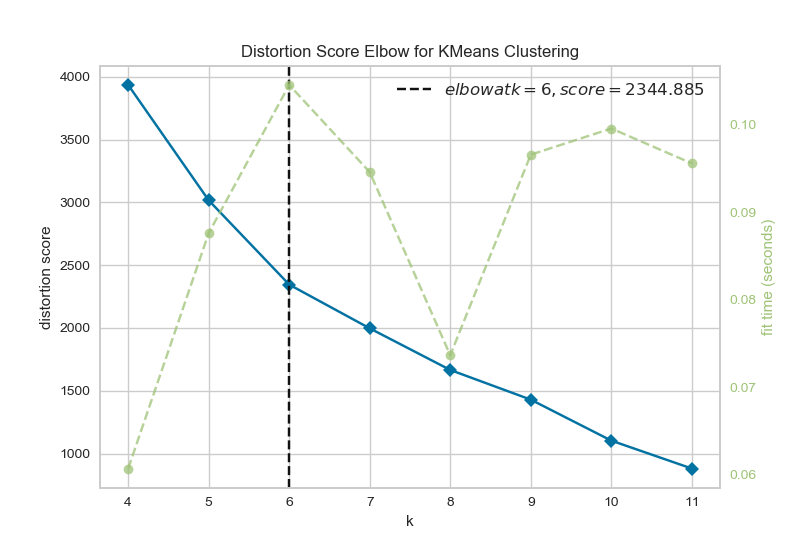
\includegraphics[width = 0.8\textwidth]{image/elbow.png}
% \caption{The elbow curve found for a $k$ range from 4 to 11 clusters. The black dotted line is optimal the number of clusters determined by the elbow method}
% \label{elb}
% \end{figure}

% The elbow method is suitable for small $k$ values. As the $k$ value increases, the average distortion degree becomes smaller. The number of data points in each category decreases, and they are closer to the center of gravity. As the $k$ value increases, the position where the improvement effect of the distortion degree decreases the most is the k value corresponding to the elbow  


\section{Streaming Cluster Analysis }
% \todo[inline]{SEQUENCE FOR THIS SECTION IS ONLINE/OFFLINE +  TIME WINDOWS +ALGORITHMS}

% \todo[inline]{start thi ssection explaining why streaming clustering is important}

\subsection{Overview}

In almost all clustering methods described in the previous section, the number of data points is considered fixed, and each data point is used multiple times for computing proximity measures and matrices in order to be assigned to a particular cluster. These methods are computationally high and require large data storage.

However, with the advent of Internet of Things, and in particular indoor localization systems, a wide range of sensor technologies (e.g., e-counters, environmental, and motion sensors) and networking communication technologies (e.g., infrared, RFID, sensors, WiFi, and Bluetooth) are being used for sensing and transporting large volumes of data. The data are harvested as data streams that are a sequence of digitally encoded coherent signals (packets of data or data packets). These data packets arrive according to different data rates (i.e. bandwidth), which are often expressed in bytes per second (B/s).

From a clustering perspective, a data stream $S$ is sequence of infinitive, ordered, and fast-changing stream data points $d_1, d_2, ..., d_3 $ $\xrightarrow S  {d_i}$ \cite{han2011data}. Therefore, clustering methods need to form clusters from a continuous flow of stream data points. The traditional set-up where an entire static data set is available for clustering can not be applied to data streams which continuously arrive at a rapid rate. The main issues can be summarized as follows \cite{toshniwal2013clustering}:

\begin{itemize}
    \item Previous data used in clustering analysis are static, but data streams are unbounded and non-stationary data.
    \item Streaming cluster analysis requires a process capable of partitioning the data streams continuously while taking into account restrictions of memory and time. Traditional clustering methods partition an entire data set at once, and memory requirements do not change over time. 
    %T \item Traditional clustering datasets can be accumulated in memory, but because of the enormous size of streaming data, it is impossible to store them in memory.. NOT SURE ABOUT THIS STATEMENT, BECAUSE WE HAVE MEMORY CONSTRAINTS WITH TRADITIONAL AS WELL AS STREAMING...
    \item Traditional clusters are found from accumulated data points, but streaming clusters evolve over time depending on the time window model being used to accumulate the data points.
\end{itemize}

It is important to select a time-interval for a time window model based on the trade-off between the data rate and latency, as that plays an important role in controlling which data points in the stream are going to be processed at the current time. Four main types of time window models have been proposed in the literature \cite{nguyen2015survey, mansalis2018evaluation}. They can be described as follows:

\begin{itemize}

    \item\textit{Damped Time Window:} It is also referred to as time-fading model. Each data point has a different weight based on its arrival time so new data points have a higher weight than the old ones. This time window model reduces the impact of old data. It is mostly applied using density-based clustering methods. The function $f(\delta t)$ = $\mu_{\delta t}$ $(0 < \mu < 1)$ is usually used for this model, where $\delta t$ is the age of a data point which is equal to time differentiation between current time and arrival time. A fading parameter $\mu$ is in the range between 0 to 1. 
    
    
    \item\textit{Landmark Time Window:} It is also known as the hopping model, and is used when clustering starts from a starting point call landmark to the current time. When a new window comes, all data points from the previous landmark time window are removed. All data points are equally important.

    \item\textit{Sliding Time Window: } The most important data points are the most recent ones and old data points will be removed. The structure of the sliding time window is based on the FIFO (First-In-First-Out) principle, in which a data point from the current time is used for clustering until a specific time is passed. The window has a size of $w$ in the current time $t$, will slide (s, sliding(w)) where s[t-w+1, t].
    The window size can be set based on resources, and computational process \cite{silva2013data}. This model is efficient when most recent data points are relevant for the cluster analysis.  
    
    \item\textit{Pyramidal Time Window: } It is also known as tilted time window and focuses on recent data points without discarding old data points. It applies various time granularity levels based on how recent a data point is \cite{aggarwal2003framework, nguyen2015survey}. It stores almost all data points belonging to a specific time window, and after computes a balance between storage requirements and accuracy. The old data tuples are aggregated. %, and a generic representation is enough.
    
\end{itemize}    

Figure   \ref{time1} illustrates how these time window models have been conceptualized. Time window models also handle concept-drift by changing the trends and data distribution in clustering, avoiding forming less accurate clusters as time passes. Finding patterns without storing all the stream data points is one of the main tasks of streaming cluster analysis.

%or data distribution over the time. It means This method aims to ignore outdated and historical data because they can change the trends or the data distribution.

\begin{figure}[!ht]
\centering
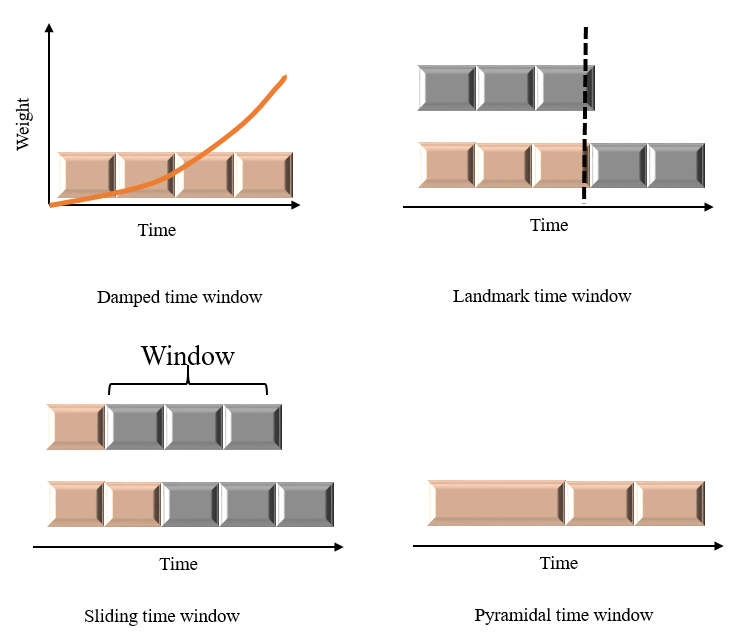
\includegraphics[width = 9cm,height = 7cm]{image/Chapters/Chapter2/timeW.PNG}
\caption{Current time window models used with stream data points \protect\cite{carnein2019optimizing}}
\label{time1}
\end{figure}


%Due to data stream volume, it is impossible to store entire objects. To control which part of data is going to be processed, time window models have been proposed. The other reason to use the time window model is to handle the concept-drift or data distribution over the time. It means This method aims to ignore outdated and historical data because they can change the trends or the data distribution.
%localization many applications and systems generate observations continuously, such as sensors, smart grids, network data, medical, finance, and so on. 
%indoor localization systems are described due to the potential wide range of services they can provide by leveraging Internet of Things (IoT) and ubiquitous connectivity.

%In order to keep changes for new data points and the possible shift in cluster structures, classical clustering algorithms need to be run periodically.  One major approach is to update existing clusters and merge new data points into the existing clusters by identifying emerging structures and removing outdated structures incrementally \cite{carnein2019optimizing}. This is the aim of data stream clustering algorithms in which data points come continuously in order, and the stream is possibly unbounded. Finding the pattern without storing all the observations is the main task of stream clustering.

% Data stream clustering finds clusters based on the flow of data points into the model, and it is different from traditional clustering \cite{toshniwal2013clustering}:
% \begin{itemize}
%     \item Traditional clustering data are static, the data stream is dynamic.
%     \item Traditional clustering datasets can be accumulated in memory, but because of the enormous size of streaming data, it is impossible to store them in memory.
%     \item traditional clustering results are fixed, but The data stream clustering results vary over time.
% \end{itemize}



%The methods that discuss the problem of data stream clustering can be categorized into: (1) one-pass methods that assume a unique underlying model of streaming data and cannotmstudy the evolution of data distribution, (2) evolving clustering methods that take into account the behavior of data as it may evolve over time.

%Many algorithms use similarity thresholds to decide whether an observation fits into an existing cluster or splitting the data space into a grid cells and store the location of dense or include fitting a model to represent the observed data.










% %%%%%%%%%%%%%%%%%%%%%%%%%%%%%%%%%%%%%

% Single-pass
% It is an array of the prototypes derived
% from k-median clustering. Because the first algorithms which
% were proposed simply view the stream clustering as a
% single-pass problem, the goal of these algorithms is to handle
% the infinite size of streams summarizing the stream history
% by dividing the stream into batches of predefined size m, in
% which each batch returns the k-representatives in the array.
% When the size of the representative array reaches the maximum
% boundary m these algorithms perform clustering in
% these k-representatives making the next level of representatives.


% single-pass means that you are supposed to process every element just once (and not copy it). Such algorithms obviously must be in linear time, which makes them good candidates for big data and MapReduce (if they can be somewhat divided, this is not necessarily trivial).

% Single-pass doesn't necessarily mean the results will be updateable and thus usable for online or streaming operation. However they often are, as they never need to access "old" data, and the summaries they are allowed to keep usually can be kept and updated.

% Single-pass are mostly interesting when you have too much data to keep or process more than once. So for "real time" applications and such. Obviously, the results will usually be worse than when you had full data available anytime


% %%%%%%%%%%%%%%%%%%%%%%%%%%%%%%%%%%%%%%%%%

%\subsection{Data Stream Processing}
Processing of data points using time window models can take two opposite views of the streaming problem as pointed out by Mansalis et al. (2018). The first view is to use a two-phase scheme which consists of an online component that processes stream data points and produces summary data  (e.g., micro-clusters, core-micro-clusters, temporal CF, grids, and coreset tree); and an offline component that uses the aggregated summary data to form the final clusters. In the literature of data stream clustering methods, a large number of algorithms use a two-phase scheme as shown in Figure \ref{2phase} . 

\begin{figure}[t]
\centering
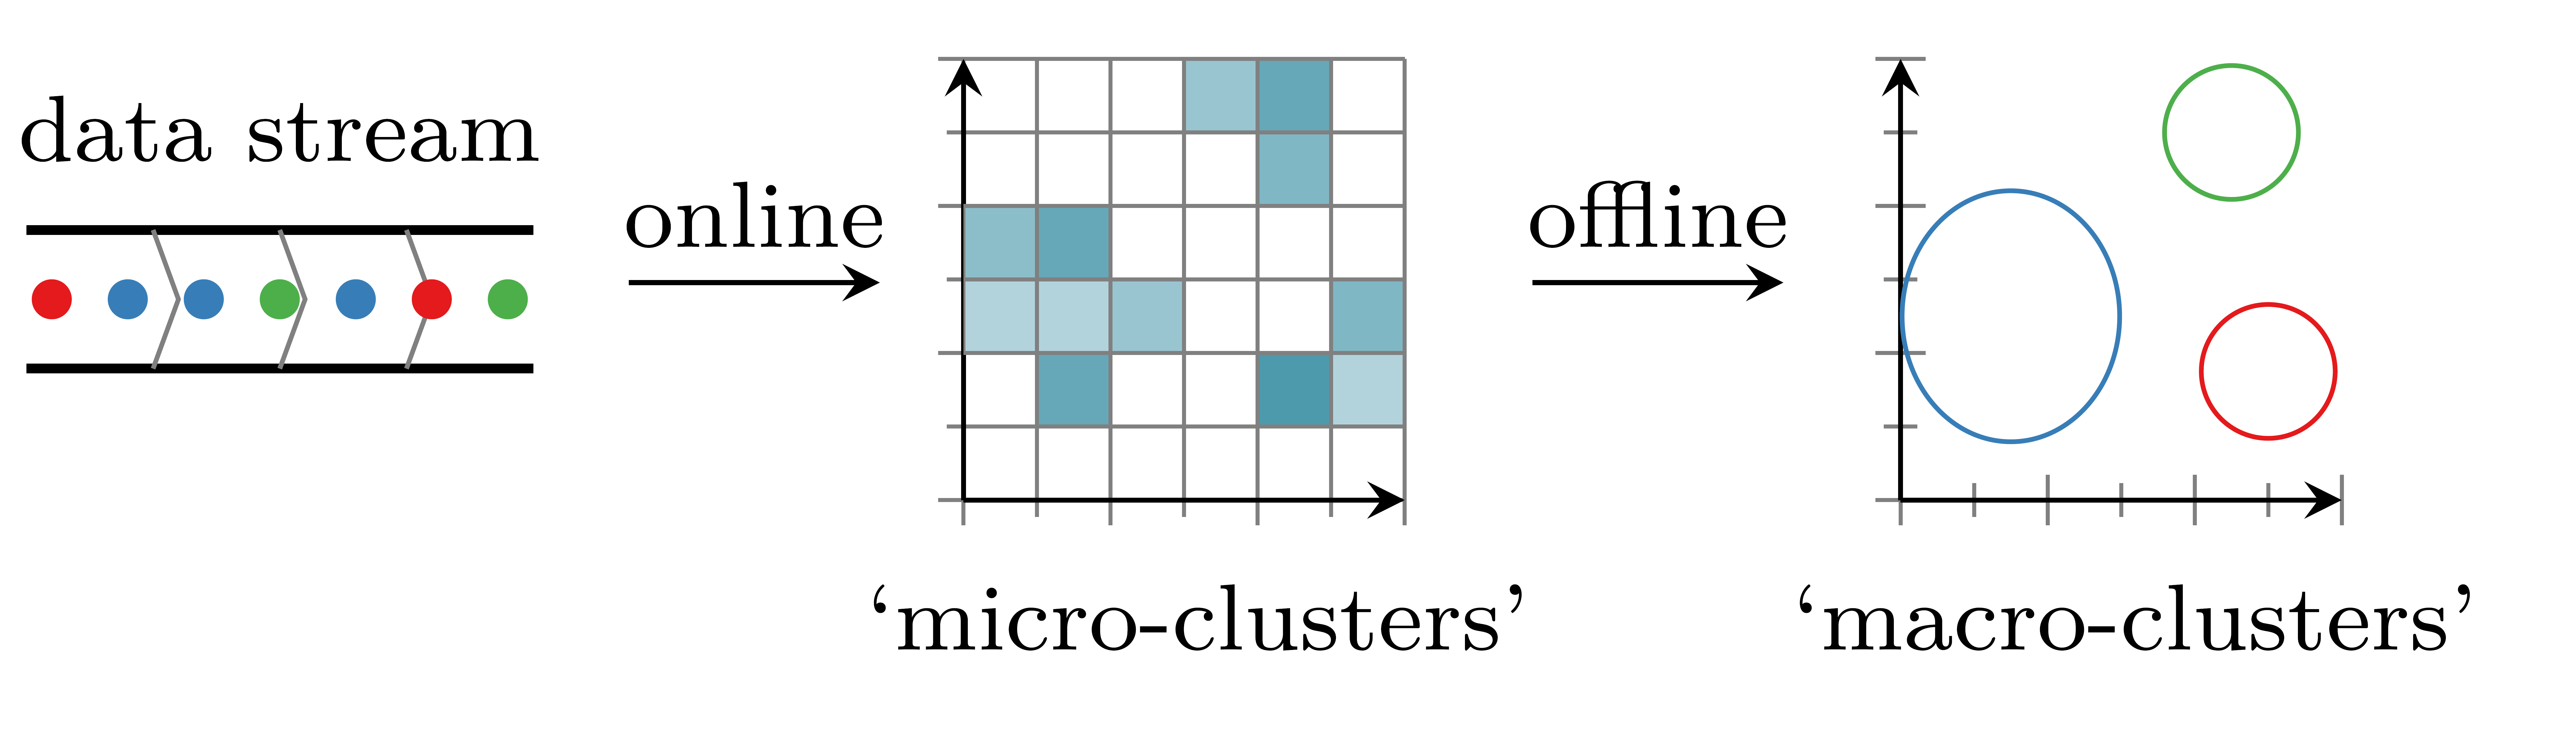
\includegraphics[width = 15cm,height = 4cm]{image/Chapters/Chapter2/2phase.png}
\caption{Overview of the two-phase processing strategy \protect\cite{carnein2019optimizing}}
%\cite{carnein2017empirical}
\label{2phase}
\end{figure}

An alternative view is to generate final clusters without the need of an offline phase. A single-pass model is maintained over a stream, and clusters are updated as new data points arrive from the stream. One of the main disadvantages of this strategy is that the evolution of the clusters can not be analyzed at different time intervals; only a final snapshot is produced.     

In this thesis, the online/offline strategy was adopted, and final clusters are referred to as macro-clusters; meanwhile the the centroids of micro-clusters were used as summary data. The online component requires a process for saving the summary data in a fast manner, and is not requested to support real-time processing, but rather a very low response delay. The offline phase uses the aggregated summary data to compute the macro-clusters. It is not time-related and can happen any time by user request.




% \begin{enumerate}
%     \item\textit{Online Clustering:}These methods observe the stream clustering problem as a single-pass clustering challenge and adopt a general adaptive strategy to maintain the clusters. This model is maintained over the stream and it is updated as new data points come from the stream. Such an approach though does not allow for investigation of the cluster structure at different time intervals.
    
    % \item\textbf{Two-phase Clustering Algorithms:} All these approaches capture the location of dense in the data space and consider them as clusters. These clusters can be merged when they become similar over time. However, it is not possible to split clusters again since the underlying data was discarded and only the center of the dense region was remained \cite{aggarwal2007data}. To avoid this issue, many clustering algorithm models are divided into two parts: online and offline phases \cite{aggarwal2003framework}. Aggarwal introduced the CluStream algorithm, combined online summarization at the first stage with the offline stage using k-means. The two-phase clustering methods are visualized in figure \ref{2phase} by the grid structure.

% \begin{figure}
% \centering
% 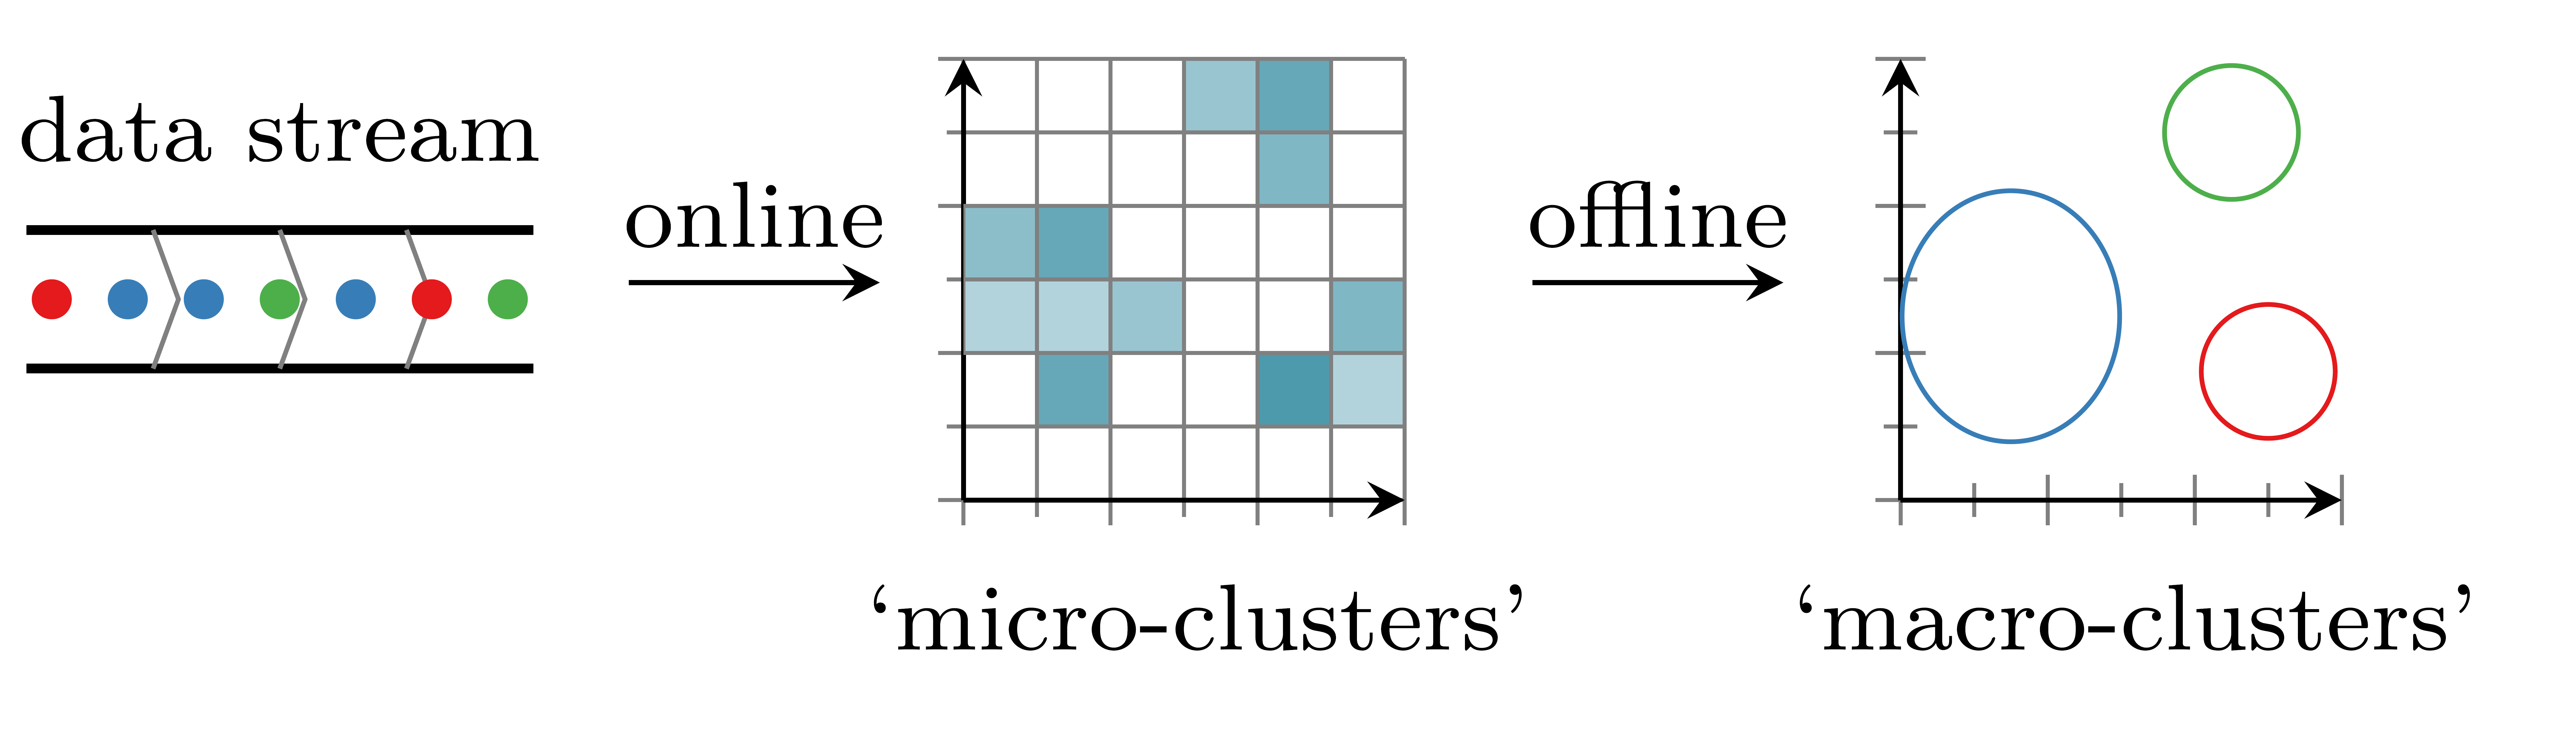
\includegraphics[width = 15cm,height = 4cm]{image/Chapters/Chapter2/2phase.png}
% \caption{Simple overview of two-phase data stream clustering algorithms \protect\cite{carnein2019optimizing}.}
% %\cite{carnein2017empirical} }
% \label{2phase}
% \end{figure}






%The second phase is triggered at the end of a designated time interval. All the centroids of clusters which have been computed by using a sliding time window model, are re-clustered to create new macro clusters and centroids. The k-means algorithm is once again employed to compute the final $k_m$ macro clusters. The advantage of applying the macro-clustering is to gain further insight from the entirety of centroids after the designated streaming window. The optimal number of $k_m$ macro clusters can be calculated by using the same method as in micro cluster which is the elbow method. The elbow method calculation can be automated or estimated at the start of micro-clustering phase. This method works by applying the k-means algorithm on micro clusters computed for all sliding time windows. 


%\subsection{Time Window Models}
\hspace{1 cm}

\subsection{Stream Clustering Methods}

Data stream clustering methods can be categorized into five leading groups according to the nature of their underlying clustering methods as previously described in Section 2.1.2. Figure \ref{method} provides an overview of the main methods developed within these categories. Table \ref{landmarkwin} provides a comprehensive overview of the data stream clustering methods. 


\begin{figure}[t]
\centering
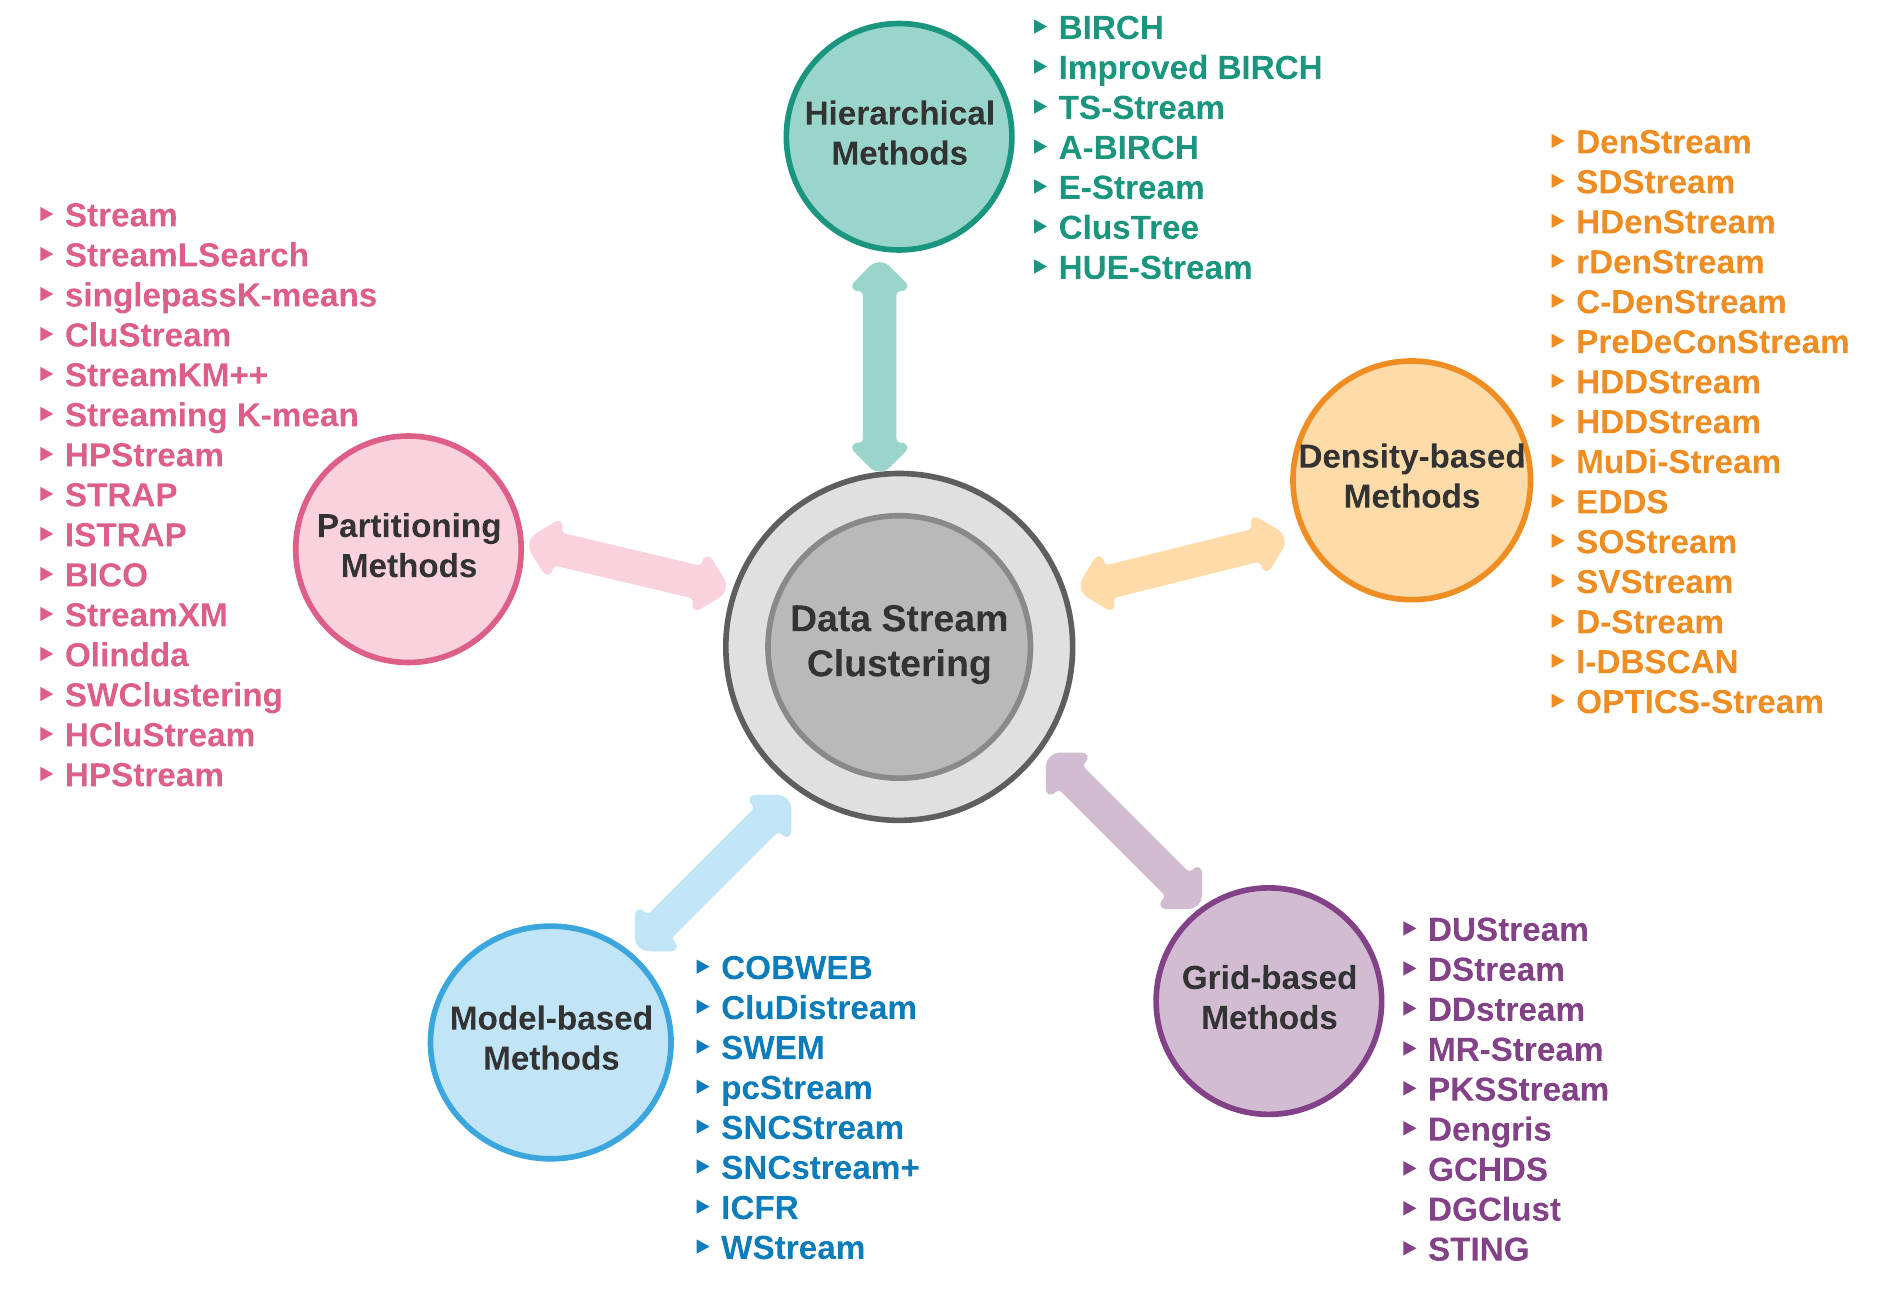
\includegraphics[width = 12 cm]{image/Chapters/Chapter2/streammethod.png}
\caption{Data stream clustering methods and algorithms}
\label{method}
\end{figure}


% \begin{itemize}
%     \item\textit{Streaming Partitioning Methods:} Table \ref{landmarkwin} provides an overview of the main methods proposed for updating the partitioning process of stream data points using landmark, sliding, and pyramidal time windows. 


%The First group is partitioning data stream clustering algorithm, which is listed in Table Table \ref{landmarkwin}. 
%As far as we had researched, no research work with affinity propagation used landmark time window model is presented.



\begin{table}[!ht]
\centering
\small
\caption{Overview of data stream clustering methods \protect\cite{mansalis2018evaluation}}
\label{landmarkwin}
\begin{tabular}{lllll}
\hline
\textbf{Algorithms} & \textbf{Year} & \textbf{Approach} & \textbf{Processing} & \textbf{Time Window} \\ \hline \midrule
\multicolumn{5}{c}{\cellcolor[HTML]{C0C0C0}\textbf{Partitioning-based}}                              \\ \hline
Stream              & 2000          & k-median          & Single-pass         & Landmark             \\ \hline
StreamLSearch       & 2002          & k-median          & Single-pass         & Landmark             \\ \hline
CluStream           & 2003          & k-means           & Online-Offline      & Pyramidal            \\ \hline
HCluStream          & 2006          & k-means           & Online-Offline      & Pyramidal            \\ \hline
Olindda             & 2007          & k-means           & Online-Offline      & Landmark             \\ \hline
SWClustering        & 2008          & k-means           & Online-Offline      & Sliding              \\ \hline
StreamKM++          & 2012          & k-means++         & Online-Offline      & Landmark             \\ \hline
BICO                & 2013          & k-means           & Online-Offline      & Landmark             \\ \hline
StreamXM            & 2015          & x-means           & Merge-reduce        & Landmark             \\ \hline
\multicolumn{5}{c}{\cellcolor[HTML]{C0C0C0}\textbf{Hierarchical-based}}                              \\ \hline
BIRCH               & 1996          & CF-tree           & Single-pass         & Landmark             \\ \hline
TS-Stream           & 2015          & Decision Tree     & Single-pass         & Sliding              \\ \hline
\multicolumn{5}{c}{\cellcolor[HTML]{C0C0C0}\textbf{Density-based}}                                   \\ \hline
DenStream           & 2006          & DBSCAN            & Online-Offline      & Damped               \\ \hline
SDStream            & 2009          & DBSCAN            & Online-Offline      & Sliding              \\ \hline
HDenStream          & 2009          & DBSCAN            & Online-Offline      & Damped               \\ \hline
FlockStream         & 2009          & Swarms            & Single-pass         & Damped               \\ \hline
rDenStream          & 2009          & DBSCAN            & Online-Offline      & Damped               \\ \hline
C-DenStream         & 2009          & C-DBSCAN          & Online-Offline      & Damped               \\ \hline
PreDeConStream      & 2012          & DBSCAN            & Online-Offline      & Damped               \\ \hline
HDDStream           & 2012          & DBSCAN            & Online-Offline      & Damped               \\ \hline
MuDi-Stream         & 2016          & DBSCAN            & Online-Offline      & Damped               \\ \hline
EDDS                & 2017          & DBSCAN            & Online-Offline      & Damped               \\ \hline
\multicolumn{5}{c}{\cellcolor[HTML]{C0C0C0}\textbf{Grid-based}}                                      \\ \hline
DUstream            & 2005          & Dense-unit        & Online-Offline      & Landmark             \\ \hline
D-stream            & 2007          & Dense-region      & Online-Offline      & Damped               \\ \hline
DDStream            & 2008          & DCQ-means         & Online-Offline      & Damped               \\ \hline
MR-Stream           & 2009          & Dense-region      & Online-Offline      & Damped               \\ \hline
PKS-Stream          & 2011          & Dense-region      & Online-Offline      & Damped               \\ \hline
DENGRIS             & 2012          & Dense-region      & Single-pass         & Sliding              \\ \hline
\multicolumn{5}{c}{\cellcolor[HTML]{C0C0C0}\textbf{Model-based}}                                     \\ \hline
COBWEB              & 1987          & Tree-based        & Online-Offline      & Landmark             \\ \hline
SWEM                & 2009          & EM Algorithm      & Online-Offline      & Sliding              \\ \hline
pcStream            & 2015          & SIMCA             & Single-pass         & Damped               \\ \hline
SNCStream           & 2015          & Network           & Online              & Damped               \\ \hline
SNCStream+          & 2016          & Network           & Online              & Damped               \\ \hline \midrule
\end{tabular}
\end{table}












% \begin{table}[h]
%     \centering
%     \caption{ Overview of data stream clustering methods \protect\cite{mansalis2018evaluation}}
%     \label{landmarkwin}
%     \small
%     \begin{tabular}{c c c c c}
%     \hline
%       \normalsize{\textbf{Algorithms} & \textbf{Year} & \textbf{ Approach } & \textbf{Processing} & \textbf{ Time Window}}  \\
%      \hline \midrule
%       \rowcolor{lightgray}& &\rowcolor{lightgray}\centering \textbf{Partitioning-based }  & &  \\
%       \hline 
%       \hline
%       Stream             &   2000    &   k-median     &  Single-pass       & Landmark \\
%      \hline
%       StreamLSearch      &   2002    &   k-median     &   Single-pass      & Landmark \\
%     \hline
%      CluStream           &   2003    &  k-means       &  Online-Offline    & Pyramidal \\
%     \hline   
%      HCluStream         &    2006   &    k-means     & Online-Offline      & Pyramidal \\
%     \hline
%      Olindda            &   2007    &   k-means      &   Online-Offline    & Landmark  \\
%     \hline    
%      SWClustering        &    2008   &    k-means     &  Online-offline    & Sliding   \\
%       \hline
%       StreamKM++         &    2012   &   k-means++    & Online-Offline     & Landmark   \\
%     \hline 
%       BICO               &    2013   &    k-means     &  Online-Offline    & Landmark  \\
%       \hline
%       StreamXM           &    2015   &    X-means     &  Merge-reduce    & Landmark  \\
%         \hline
%       \hline
%       \rowcolor{lightgray}&& \rowcolor{lightgray}\centering\textbf{Hierarchical-based }  & &  \\
%       \hline 
%       \hline 
%       BIRCH             &    1996        &     CF-tree           &  Single-pass    & Landmark \\
%      \hline
%       TS-Stream         &     2015       &    Decision Tree      & Single-pass     & Sliding  \\
%       \hline
%       \hline
%      \rowcolor{lightgray}& &\rowcolor{lightgray}\centering \textbf{Density-based}  & &  \\
%       \hline 
%       \hline
%     DenStream            &    2006     &    DBSCAN       & Online-offline  &   Damped   \\
%      \hline
%      SDStream            &    2009     &    DBSCAN       & Online-offline  &   Sliding \\
%       \hline
%       HDenStream         &     2009    &    DBSCAN       &  Online-offline &   Damped  \\
%         \hline
%       FlockStream        &     2009    &    Swarms       &  Single-pass    &   Damped  \\
%         \hline 
%       rDenStream         &    2009     &     DBSCAN      & Online-offline  &   Damped  \\
%         \hline 
%       C-DenStream        &    2009     &     C-DBSCAN    &Online-offline   &   Damped \\
%           \hline 
%       PreDeConStream     &    2012     &     DBSCAN      & Online-offline  &   Damped \\
%           \hline 
%       HDDStream          &    2012     &     DBSCAN      & Online-offline  &   Damped   \\
%           \hline 
%       MuDi-Stream        &    2016     &       DBSCAN    & Online-offline  &   Damped\\
%       \hline          
%       EDDS               &    2017     &     DBSCAN      & Online-offline  &   Damped \\
%       \hline
%       \hline
%      \rowcolor{lightgray}& &\rowcolor{lightgray}\centering \textbf{Grid-based}  & &  \\
%       \hline 
%       \hline      
%      DUstream            &    2005        &      Dense-unit       &     Single-pass    &  Landmark\\
%       \hline
%       D-stream           &     2007       &    Dense-region       &  Online-offline    &   Damped\\
%     \hline 
%       DDStream           &    2008        &    DCQ-means          &     Online-offline & Damped \\
%     \hline 
%       MR-Stream          &    2009        &     Dense-region      &  Online-offline    & Damped\\
%     \hline 
%       PKS-Stream         &    2011        &    Dense-region       &  Online-offline    & Damped\\
%     \hline 
%       DENGRIS            &    2012        &   Dense-region        &  Single-pass       & Sliding\\
%       \hline 
%       \hline
%      \rowcolor{lightgray}& &\rowcolor{lightgray}\centering\textbf{Model-based}  & &  \\
%       \hline 
%       \hline
%       COBWEB             &    1987        &   tree-based      &    Online-offline   & Landmark \\
%      \hline
%       SWEM               &    2009        &  EM Algorithm     &  Online-offline     & Sliding\\
%      \hline
%      pcStream            &    2015        &    SIMCA          &   Single-pass       & Damped  \\
%     \hline 
%       SNCStream          &    2015        &    Network        &   Online            & Damped  \\
%     \hline 
%     SNCStream+      &    2016        &       Network     &    Online           & Damped  \\
      
% \bottomrule
%     \end{tabular}
% \end{table}

In this research work, the DSAP algorithm is proposed as a simplification of the previous streaming AP algorithms. This is further discussed in the next chapter.


% In particular, the online-offline processing for streaming K-means clustering has been applied to many algorithms such as CluStream, Olindda, SWClustering, and BICO. The open-source available DSC\_TwoStage in R version of streaming K-means using the 2-phase processing was used in this thesis, and is further discussed in Chapter 5.  



% The Stream algorithm proposed by Guha et al. \cite{o2002streaming} is one of the earliest approaches in this field. This method is the k-median approach and divides the stream into batches of data with a fixed size. At each batch, the k-median algorithm is applied. 


% Olindda introduced by Spinosa \cite{spinosa2007olindda}, based on the K-means clustering algorithm, is an online anomaly detection algorithm. Olindda continuously monitors and adapts to emerging data distributions. Unknown samples are kept in a memory queue and are periodically clustered and then either merged with an existing similar cluster or added as a novel cluster to the pool of clusters.
% This model calculates the maximum distance between data points and centroids as a decision boundary (threshold) for each cluster. The union of the boundaries of all clusters is the global decision boundary that defines the model. A new unseen data point that falls inside this boundary is consistent with the model and therefore considered normal. Otherwise, This specific data point is labeled as an unknown and separated for further analysis.
% %similar to my work
% CluStream \cite{aggarwal2003framework} is inherited from the BIRCH algorithm. The online phase is started by applying the k-means algorithm to create micro-clusters. When a new data point arrives, it is absorbed by its closest micro-cluster if it fit within an adaptive radius threshold. Otherwise, it creates a new cluster. To keep micro-clusters in some range, expired clusters are removed based on a threshold on their average time stamp. If it cannot happen, the two closest micro-clusters will be merged.
% To support different time-horizons, CluStream frequently collects snapshots of the current CFs by a pyramidal time frame. 

% Another algorithm is HCluStream \cite{yang2006hclustream} is an extension of CluStream for categorical data by storing the frequency of attribute-levels for all categorical features. This algorithm creates a  categorical distance measure separately to combine with the traditional distance measure for continuous attributes.

% SWClustering \cite{zhou2008tracking} introduced a new data structure for this algorithm called Exponential Histogram of Cluster Feature (EHCF), which can handle cluster evolution and represents the changes of the cluster distribution and capture it. In the online phase, it captures objects as synopses in the EHCF structure, and in the offline phase, the algorithm clusters these collections of synopses using a k-means algorithm.

% Ackermann et al. \cite{ackermann2012streamk} develop a new coreset construction for the Euclidean k-means clustering problem and called it StreamKM++. A coreset is a small weighted point set that approximates the original input point set with respect to a given optimization problem. This algorithm proposed a coreset construction for the Euclidean k-means clustering problem called coreset tree suitable for high dimensional data. Then, they used a standard streaming technique, called the merge-and-reduce technique, to maintain observation in data streams. After processing the whole input stream, the k-MEANS++ algorithm applies to obtain a k-means clustering and celled it the StreamKM++ algorithm.

% BICO \cite{fichtenberger2013bico} is another algorithm in this group that combines the BIRCH data structure with StreamKM++. 






%\item\textbf{Hierarchical-based algorithms:}

% \begin{table}[h]
%     \centering
%     \caption{Overview of Hierarchical-based stream clustering algorithms. }
%     \label{hirarcha}
%     \small
%     \begin{tabular}{c c c c c}
%     \hline
%       \textbf{Algorithms} & \textbf{Year} & \textbf{ Method } & \textbf{Processing} & \textbf{ Time Window}  \\
%      \hline \midrule

%       BIRCH             &    1996        &     CF-tree  &         & Landmark \\
%      \hline
%      Improved BIRCH     &    2014        &    CF-tree   &         & Landmark \\
%       \hline
%       TS-Stream         &     2015       &    -      &       & Sliding  \\
%     \hline 
%       A-BIRCH           &    2017        &   CF-tree    &      & Landmark\\
% \bottomrule
%     \end{tabular}
% \end{table}

%BIRCH \cite{zhang1996birch} is one of the earliest stream clustering algorithms. This algorithm minimizes large datasets' memory requirements by summarizing the information contained in dense regions as Clustering Feature (CF) entries. CF has three components: the number of data points, the d-dimensional vector with the linear sum of all data points, and a sum of squares for all data points across dimensions. BIRCH incrementally builds a balanced-tree to maintain CFs, where each node can contain a fixed number of CFs. 
%For every new data point that comes into the model, the tree descends by following the child to its closest CF until a leaf node is reached. The new data point can either merged to its closest leaf-CF or creates a new leaf-CF. This method has a significant drawback which is the limited capacity of its leaves.

% Improved BIRCH \cite{ismael2014improved} is an extension of the BIRCH algorithm, which employs various distance thresholds per CF.

% TS-Stream \cite{pereira2014ts} is a time-series data stream clustering with the time frame. 

% A-BIRCH \cite{lorbeer2016birch} is similar to Improved BIRCH, determines the threshold parameters by using the Gap Statistics on a representation of the stream.



% \item\textbf{Density-based algorithms:}

% \begin{table}[h]
%     \centering
%     \caption{Overview of Density-based stream clustering algorithms. }
%     \label{densalgo}
%     \small
%     \begin{tabular}{c c c c c}
%     \hline
%       \textbf{Algorithms} & \textbf{Year} & \textbf{ Time window } & \textbf{Method} & \textbf{ Processing}  \\
%      \hline \midrule

%       DenStream          &    2006        &    Damped          &    DBSCAN      & Online-offline \\
%      \hline
%      SDStream            &    2009        &    Sliding         &    DBSCAN      & Online-offline \\
%       \hline
%       HDenStream         &     2009       &     Damped         &    DBSCAN      &  Online-offline \\
%         \hline 
%       rDenStream         &    2009        &    Damped         &     DBSCAN      & Online-offline \\
%         \hline 
%       C-DenStream        &    2009        &    Damped         &     C-DBSCAN    &Online-offline \\
%           \hline 
%       PreDeConStream     &    2012        &   Damped          &     DBSCAN      & Online-offline\\
%           \hline 
%       HDDStream          &    2012        &   Damped          &     DBSCAN      & Online-offline\\
%           \hline 
%       EDDS               &    2017        &   Damped          &     DBSCAN      & Online-offline\\
% \bottomrule
%     \end{tabular}
% \end{table}

% DenStream \cite{cao2006density} is the temporal extension of the CFs from the BIRCH algorithm with having core micro cluster using time-faded CF. This algorithm was implemented with arbitrary shape data.

% SDStream \cite{ren2009density} is a variant of DenStream algorithm for sliding time window model. This algorithm keeps CMCs in the form of an Exponential Histogram.
 
% HDenStream \cite{lin2009density} is a combination of DStream (with the categorical distance measure ) and HCluStream for categorical datasets. 

% FlockStream \cite{forestiero2013single} applies a flocking behavior to identify emerging flocks and swarms of objects. Like the DenStream algorithm, FlockStream differentiates between potential core and outlier micro-clusters and uses a time-faded CF. 

% rDenStream \cite{liu2009rdenstream} to detects outliers,  this algorithm temporarily stores them away in an outlier buffer.  After the offline phase, the algorithm tries to re-cluster the data points cached in the buffer to improve the clustering.

% C-DenStream \cite{ruiz2009c} is another type of  DenStream that allows domain knowledge in instance-level constraints into the clustering method. Instance-level constraints mean data points that can or cannot belong to the same cluster.

% PreDeConStream \cite{hassani2012density} was implemented simultaneously to HDDStream. The algorithm changes in regular intervals by applying a modified PreDeCon algorithm on the micro-clusters generated during the online phase.

% HDDStream \cite{ntoutsi2012density}

% \item\textbf{Grid-based algorithms:}
% Grid-based algorithms capture the density in the grid. Macro-clusters are usually obtained by grouping adjacent dense cells. How to make a grid cell is very challenging. Table \ref{gridd} shows the overview of some main algorithms in this group. The most popular grid-based algorithm is DStream \cite{chen2007density}.


% \begin{table}[h]
%     \centering
%     \caption{Overview of grid-based stream clustering algorithms. }
%     \label{gridd}
%     \small
%     \begin{tabular}{c c c c c}
%     \hline
%       \textbf{Algorithms} & \textbf{Year} & \textbf{ Method } & \textbf{Processing} & \textbf{ Time Window}  \\
%      \hline \midrule

%       Fractal Clustering &    2000        &                       &  Online            &   Landmark\\
%           \hline 
%      DUstream            &    2005        &      Dense-unit       &     Online         &  Landmark\\
%       \hline
%       Dstream            &     2007       &    Dense-region       &  Online-offline    &   Damped\\
%     \hline 
%       DDStream           &    2008        &    DCQ-means          &     Online-offline & Damped \\
%     \hline 
%       MR-Stream          &    2009        &     Dense-region      &  Online-offline    & Damped\\
%     \hline 
%       PKS-Stream         &    2011        &    Dense-region       &  Online-offline    & Damped\\
%           \hline 
%       DENGRIS            &    2012        &   Dense-region        &  Online            & Sliding\\
%           \hline 
%       HDCStream          &    2014        &                       &    Online          & Damped\\
%           \hline 
%       MuDi-Stream        &    2016        &       DBSCAN          & Online-offline      & Damped\\
% \bottomrule
%     \end{tabular}
% \end{table}

% Dstream has a fixed grid size, with three different types of cells: dense cells, sparse cells, and transitional cells, which it is categorized between the other two types. The algorithm outlines new data points to its corresponding cell and is initialized by assigning all dense cells to individual clusters. These clusters are extended with all neighboring transitional grids or merged with neighboring dense cell clusters. In any intervals, the clustering assesses the weight of individual cell and includes the
% changes in cell types into the clustering.


% DUstream \cite{gao2005incremental} devides the data space once into fixed grid-cells.
% The algorithm processes the first part of data to start the clustering and maintains all cells with sufficient density. The density of cells is determined, corresponding to the total number of observations. 

% DDstream \cite{jia2008grid} is an extension of points that lie precisely on the grid boundaries. For these points, the distance to adjacent cell centers is calculated, and those points are assigned to their closest cell. 





% \item\textbf{Model-based algorithms:}
% This group of algorithms summarize the data stream as a statistical model, usually based on Expectation Maximization (EM) algorithm. 

% \begin{table}[h]
%     \centering
%     \caption{Overview of model-based stream clustering algorithms. }
%     \label{modealgo}
%     \small
%     \begin{tabular}{c c c c c}
%     \hline
%       \textbf{Algorithms} & \textbf{Year} & \textbf{ Method } & \textbf{Processing} & \textbf{ Time Window}  \\
%      \hline \midrule

%       COBWEB             &    1987        &   tree-based   &          & Landmark \\
%      \hline
%      WStream             &    2004        &   Kernel-density  &                     & Damped \\
%       \hline
%       CluDistream        &     2007       &   EM           &        &  Landmark \\
%     \hline 
%       SWEM               &    2009        &  EM            &  Online-offline      & Sliding\\
%     \hline 
%       SVStream          &    2013         &    SVC         &                     & Damped  \\
%     \hline 
%       pcStream          &    2015         &       SIMCA    & Online        & Damped  \\
% \bottomrule
%     \end{tabular}
% \end{table}


% COBWEB \cite{fisher1987knowledge} is a tree-based algorithm, and each node describes a cluster. Tree incrementally builds by descending a new entry from the root to a leaf. 

% WStream \cite{tasoulis2006unsupervised} uses kernel density to keeps several windows in the data space. It means to use the local maxima of a density estimate as cluster centers and the local minima as cluster boundaries. New data points can add to an existing window, or it is used to initialize a new window with the default size. 

% CluDiStream \cite{zhou2007distributed} applies EM algorithm for data stream clustering. This algorithm learns the distribution of underlying data streams by maximizing the likelihood of the data clusters. It keeps the distribution of Gaussian mixture and a coordinator node in each location to combine the distributions.

% SWEM \cite{dang2009based} uses EM to chunks of data with random initial parameters. Distributions for the first chunk of data calculates. Each cluster is then summarized using a CF and macro-clusters by applying EM again.

% SVStream \cite{wang2011svstream} is based on support vector clustering (SVC), which transforms the data into the higher dimensional space. The model is run in chunks, and the first one runs SVC. For other chunks, it checks if it is in the radius of spheres or not. If yes, a new sphere is initialized. 






% \end{itemize}

% \subsection{Streaming k-means clustering}

% move things from the other chapters(s) to here
% look at the thesis from Luke to describe the method. the only [platform we have is R]
   	    
% Streaming clustering with K-means is employed to provide fast responses where new data points coming into the data stream are analyzed near real-time instead of applying as an traditional K-means method for a particular dataset. Different type of stream clustering with K-means are available during the history of stream clustering. 

% to keep the clustering computational effort beyond reasonable limits for large-scale data in an online fashion, divide and conquer approach is deployed by using K-means traditional algorithm \cite{nittel2004scaling}. 
% This approach has mainly three steps as shown in Figure \ref{dividee}: partitioning the dataset into different chunks, then clustering each chunk and find the results, lastly, computes the results out of all chunks of data. 

% \begin{figure}[!h]
%     \centering
%     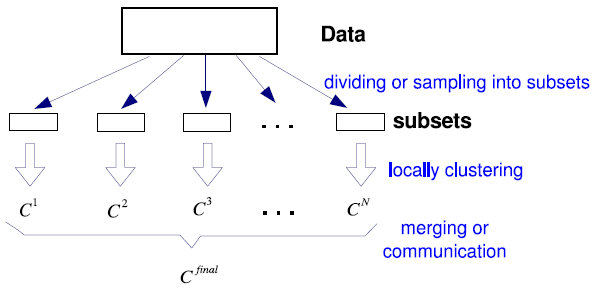
\includegraphics[width = 11 cm]{image/Chapters/Chapter3/divide.PNG}
%     \caption{Divide and conquer approach to generate clustering out of big data \protect\cite{zhang2009toward}}
%     \label{dividee}
% \end{figure}   	    
% \cite{khalilian2016data} 
% The query processing cost for such a method is high, and it does not work for applications that require fast query response. Remarkably, they require merging multiple data structures at the time of query, followed by an extraction of cluster centers, which is expensive \cite{zhang2017streaming}.

% The online and offline streaming K-means clustering approach has applied on different algorithms such as CluStream, Olindda, SWClustering, BICO. 



% The open-source available version of streaming K-means is DSC\_TwoStage in R programming language. 




% \begin{algorithm}[H]
% \SetAlgoLined
% \textbf{Input:} Data stream $S=(s_{1}, s_{2},...,s_{n})$, number of micro clusters $k$, number of macro cluster $k_m$, sliding time window $W$ with the size $z$;\\
% \textbf{Output:} {Set of micro clusters $C_m= (C_{m_1}, C_{m_2}, ..., C_{m_k})$, and set of macro clusters $C_M= (C_{M_1}, C_{M_2}, ..., C_{M_{k_m}})$ }\\
% \SetKwFunction{FIROC}{Streaming K-means}
% \SetKwProg{Fn}{Function}{:}{}
% \Fn{\FIROC{S, W}}{
         
% \textbf{Initialization:}
% \begin{itemize}
%     \item Partition S with $W$ into k subsets $S_1$, . . . , $S_k$, such that $S_i$, 1 $\leq$ i $\leq$ k,
%     \item Extract $W_1$ = $(s_1...s_z)$ data points from $S$
%     % \item partition S with $W$ into k subsets $S_1$, . . . , $S_k$
%     \item Estimate $k$ initial centroids $c_1, . . . , c_k$ from $W_1$ using K-means
% \end{itemize}

% \Repeat{Centroid convergence is achieved}{          
%  \SetKwFunction{FIROC}{K-means}         \hfill \Comment{Online Phase}\\
% \SetKwProg{Fn}{Function}{:}{}
% \Fn{\FIROC{Wi,k}}{
%  Assign data points $s_i$ to the closest centroid\\
%  Replace the current centroids by new centroids $c_1, ..., c_i$\\}
% \textbf{return}{ $(C_{m_1}, C_{m_2}, ..., C_{m_k})$ }\\
% }

% \Repeat{Centroids convergence happens}{
%   \SetKwFunction{FIROC}{K-means}         \hfill \Comment{Offline Phase}\\
% \SetKwProg{Fn}{Function}{:}{}
% \Fn{\FIROC{C_m,k_m}}{                                     
%   Find $k_m$ macro clusters from $C_m$ centroids\\
%   }
% }

% \textbf{return} {macro clusters: $C_{M_1}, C_{M_2}, ..., C_{M_{k_m}}$\\ }
% }
%  \caption{Streaming K-means Online Micro and Offline Macro Clustering Algorithm}
% \end{algorithm}


%New ideas continue evolving in data streams over time. Evolving needs updating data stream algorithms to adjust to the changes such as handle well rapid cluster evolution patterns.







%%%%%%%%%%%%%%%%%%%%%%%%%%%%%%%%%%%%%%%%%%%%%%%%%%%%%%chapter 4
% \section{online- offline clustering}
% This section introduced a three phase, online micro, offline macro, and evaluation streaming K-means algorithm for comparison with the proposed DSAP algorithm. The streaming K-means algorithms are  widely used to analyze streaming data. In this section, the framework of streaming K-means algorithm is discussed. As shown earlier in Figure \ref{wrk1} the DSAP and streaming K-means algorithms have analogous phases with the major differences in the clustering algorithm.
% \subsection{Online Micro-Clustering Phase}
% In this phase, the data stream arrives are accumulated using the sliding time window model. The streaming K-means model incrementally updates when a new data window comes into the model to generate the micro clusters. These points can also be clustered using K-means with preferred $k$ cluster centroids. The approach used for selecting the $k$ number of micro clusters is the elbow method described previously in section \ref{elbowmethod}. The algorithm randomly chooses $n$ data points in each time frame until convergence happens. It computes the sum of the squared distances from each data point to its assigned centroid.

% \begin{figure}
% \centering
% 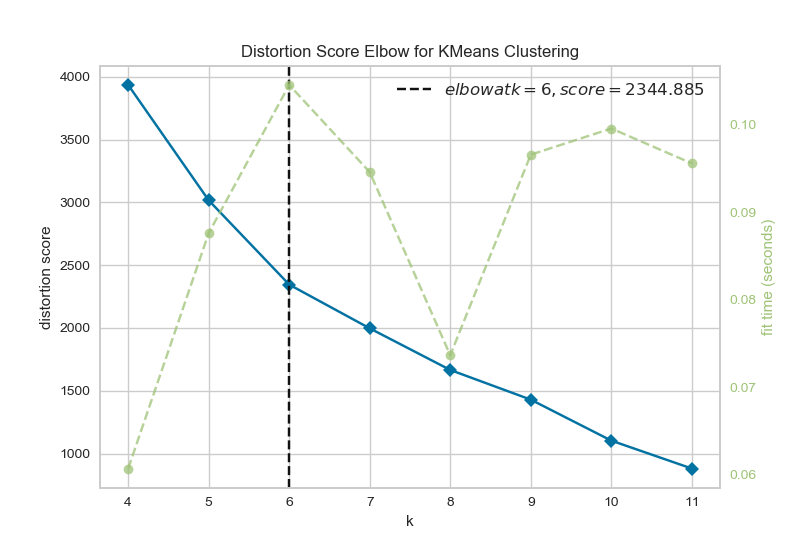
\includegraphics[width = 12cm,height = 8cm]{image/elbow.png}
% \caption{The elbow curve found for a $k$ range from 4 to 11 clusters. The black dotted line is the number of clusters determined by the elbow method}
% \label{elb}
% \end{figure}




%\subsection{Streaming K-means Clustering Performance Evaluation}
%The quality and efficiency of the streaming K-means clustering algorithm need to be evaluated as well as the DSAP algorithm. The quality of clusters found by each algorithm are assessed by these four criteria: Silhouette Coefficient, Calinski-Harabasz Index, Davies-Bouldin Index and outlier detection.
%The efficiency is compared using three metrics: computational time efficiency, frequency of the outliers and the memory consumed to run the program.



%\subsubsection{Evaluation of Data Stream Clustering}

%In data stream clustering (DSC) phase, stream currently provides moving windows and sampling from a stream as data stream operators.DSC\_Window provides a clustering interface to the data stream. It implements the sliding window and the dampened window models which keep a user-specified number (window length) of the most recent data points of the stream. For the dampened window model, data points in the window have a weight that deceases exponentially with age.
%%%elmi
%Evaluating the performance of a clustering algorithm is not counting the number of errors or accuracy. In particular, any evaluation metric if this clustering defines separations of the data similar to some ground truth set of classes or satisfying some assumption such that members belong to the same class are more similar than members of different classes according to some similarity metric.The main purpose of clustering methods is to find high intra-cluster similarity and low inter-cluster similarity. In a simple term, objects in the same cluster are more similar than the objects in different clusters.
%%




%%%%%%%%%%%%%%%%%%%%%%%%%%%%%%%%%%%%%%%%%%%%%%%%%%%%%%%%%%%%%%%%%%%%%%%%%%%%%%% KEEP
% \section{Sliding Time Window Model}
% The sliding time window model limits the scope of data to a sequence of the most recent data points in the data stream to compute the micro clusters, since the new data point is available, the old one is removed.
% The first window is started with a pre-defined time frame based on the data, and this window containing the accumulated data points from where the stream started. After a new data point arrives, the algorithm updates the micro clusters incrementally each time. Next, the new time window employs all the new data points and clusters as the data points, saving the new micro clusters and the selected centroids. 

% By applying a sliding time window model, the sum of square distances will often eliminate at a local optimum. Accordingly, it leads to the micro-clustering evolution results. The main focus is finding micro clusters evolution to identify new clusters from outliers. There are two types of sliding windows, time-based and count-based sliding windows \cite{li2014parallel}. In time-based sliding windows, time intervals are applied(e.g., every 10 minutes), while in count-based sliding windows, they are defined in terms of the number of data points. Figure \ref{stw} shows sliding time window model with the data points included in a window.  Equation \ref{eq11} shows the calculation of time window:
% \begin{equation}
%     W_i = [m_i, ..., m_{(i+w-1)}]\label{eq11}
% \end{equation}

% Where $w$ is a window length, $m_i$ is the $i^{th}$ data point and $W_i$ is the $i^{th}$ window. 
% \begin{figure}
% \centering
% %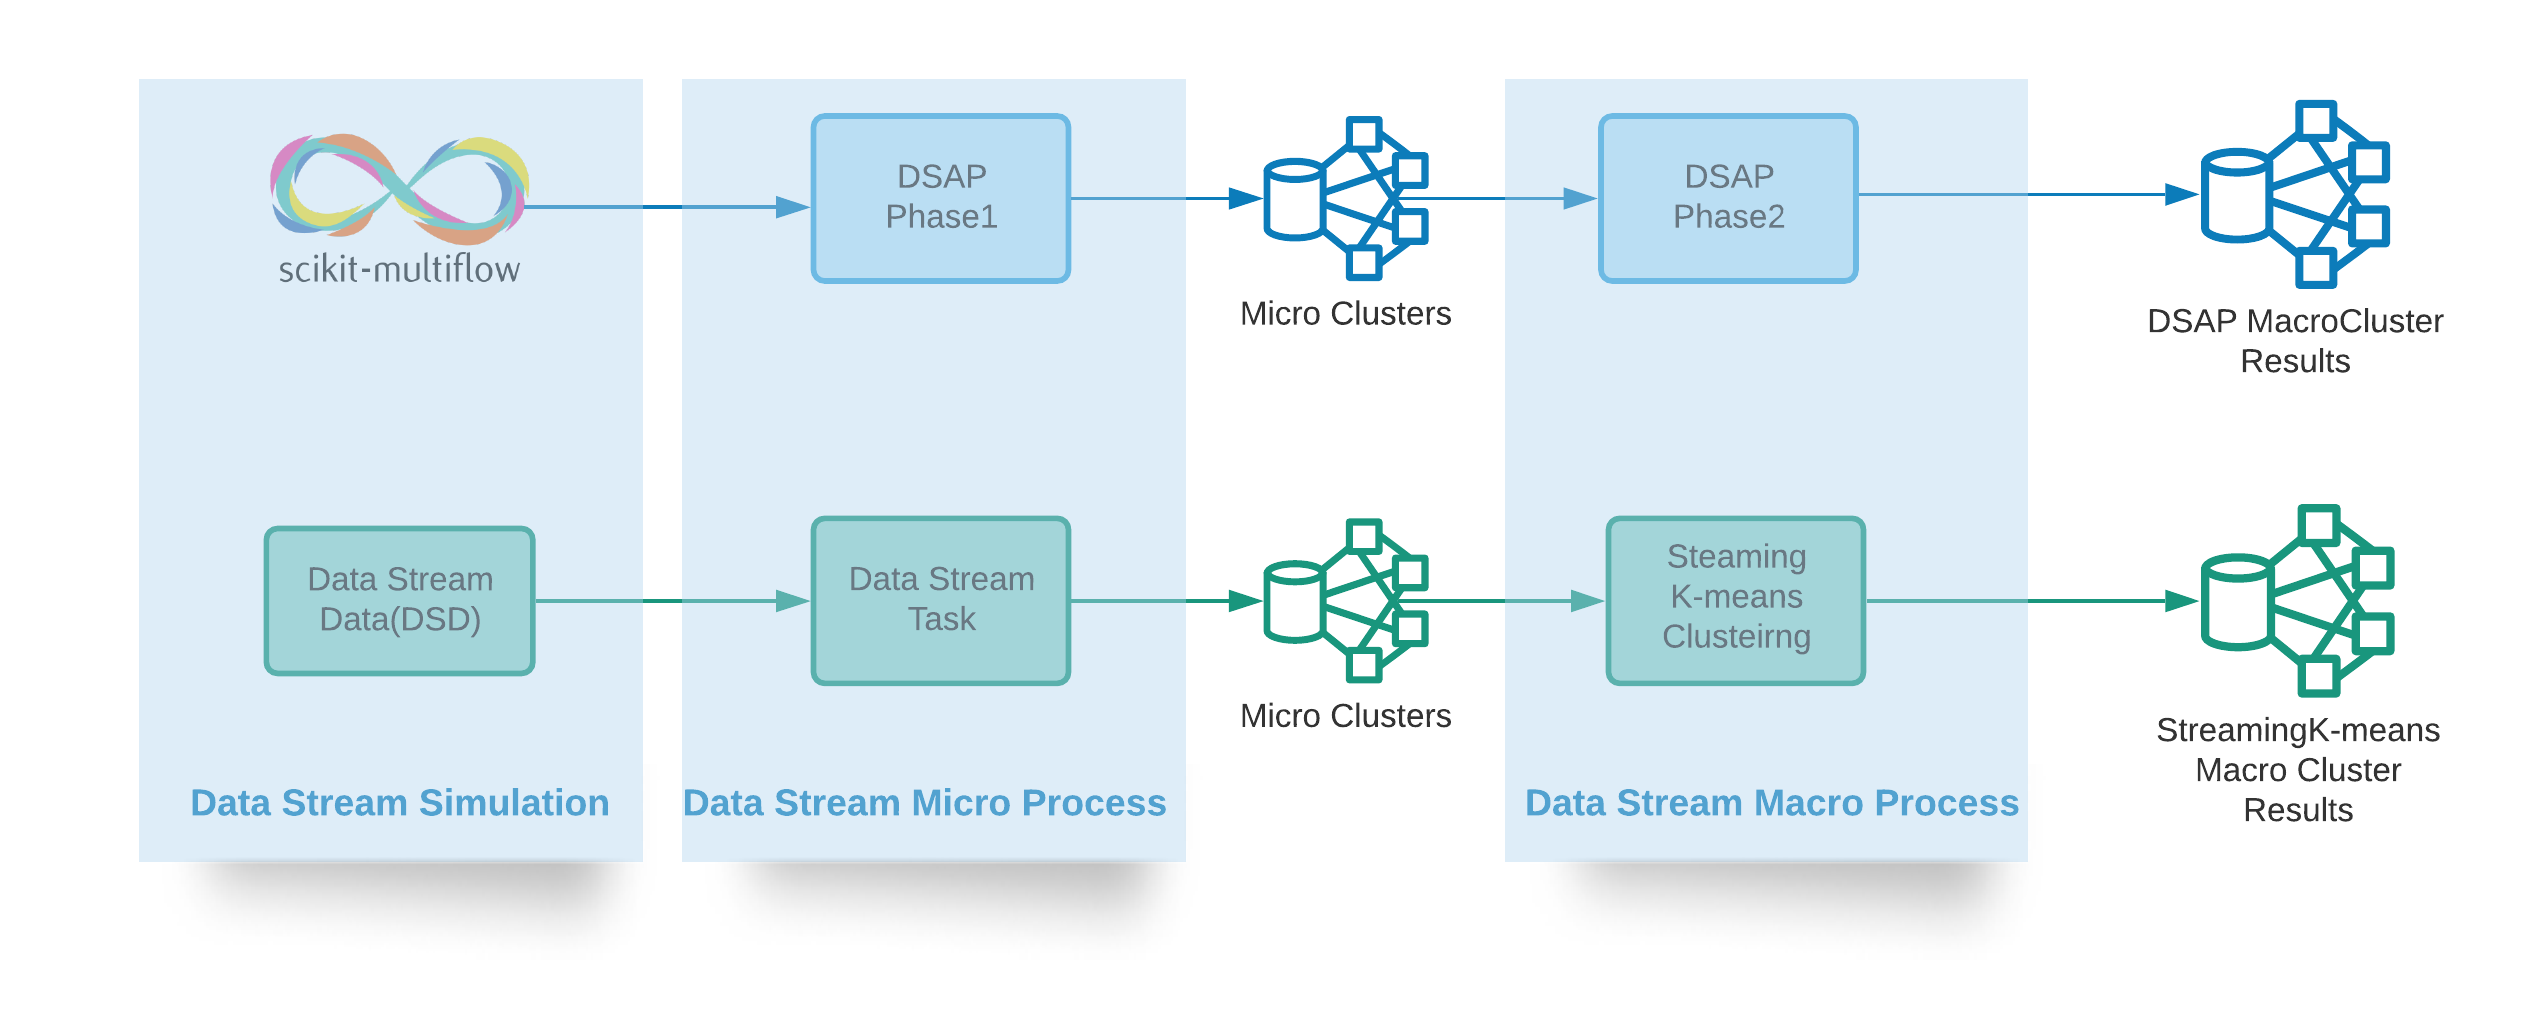
\includegraphics[width = 15cm,height = 7cm]{image/2-2workflow.png}
% 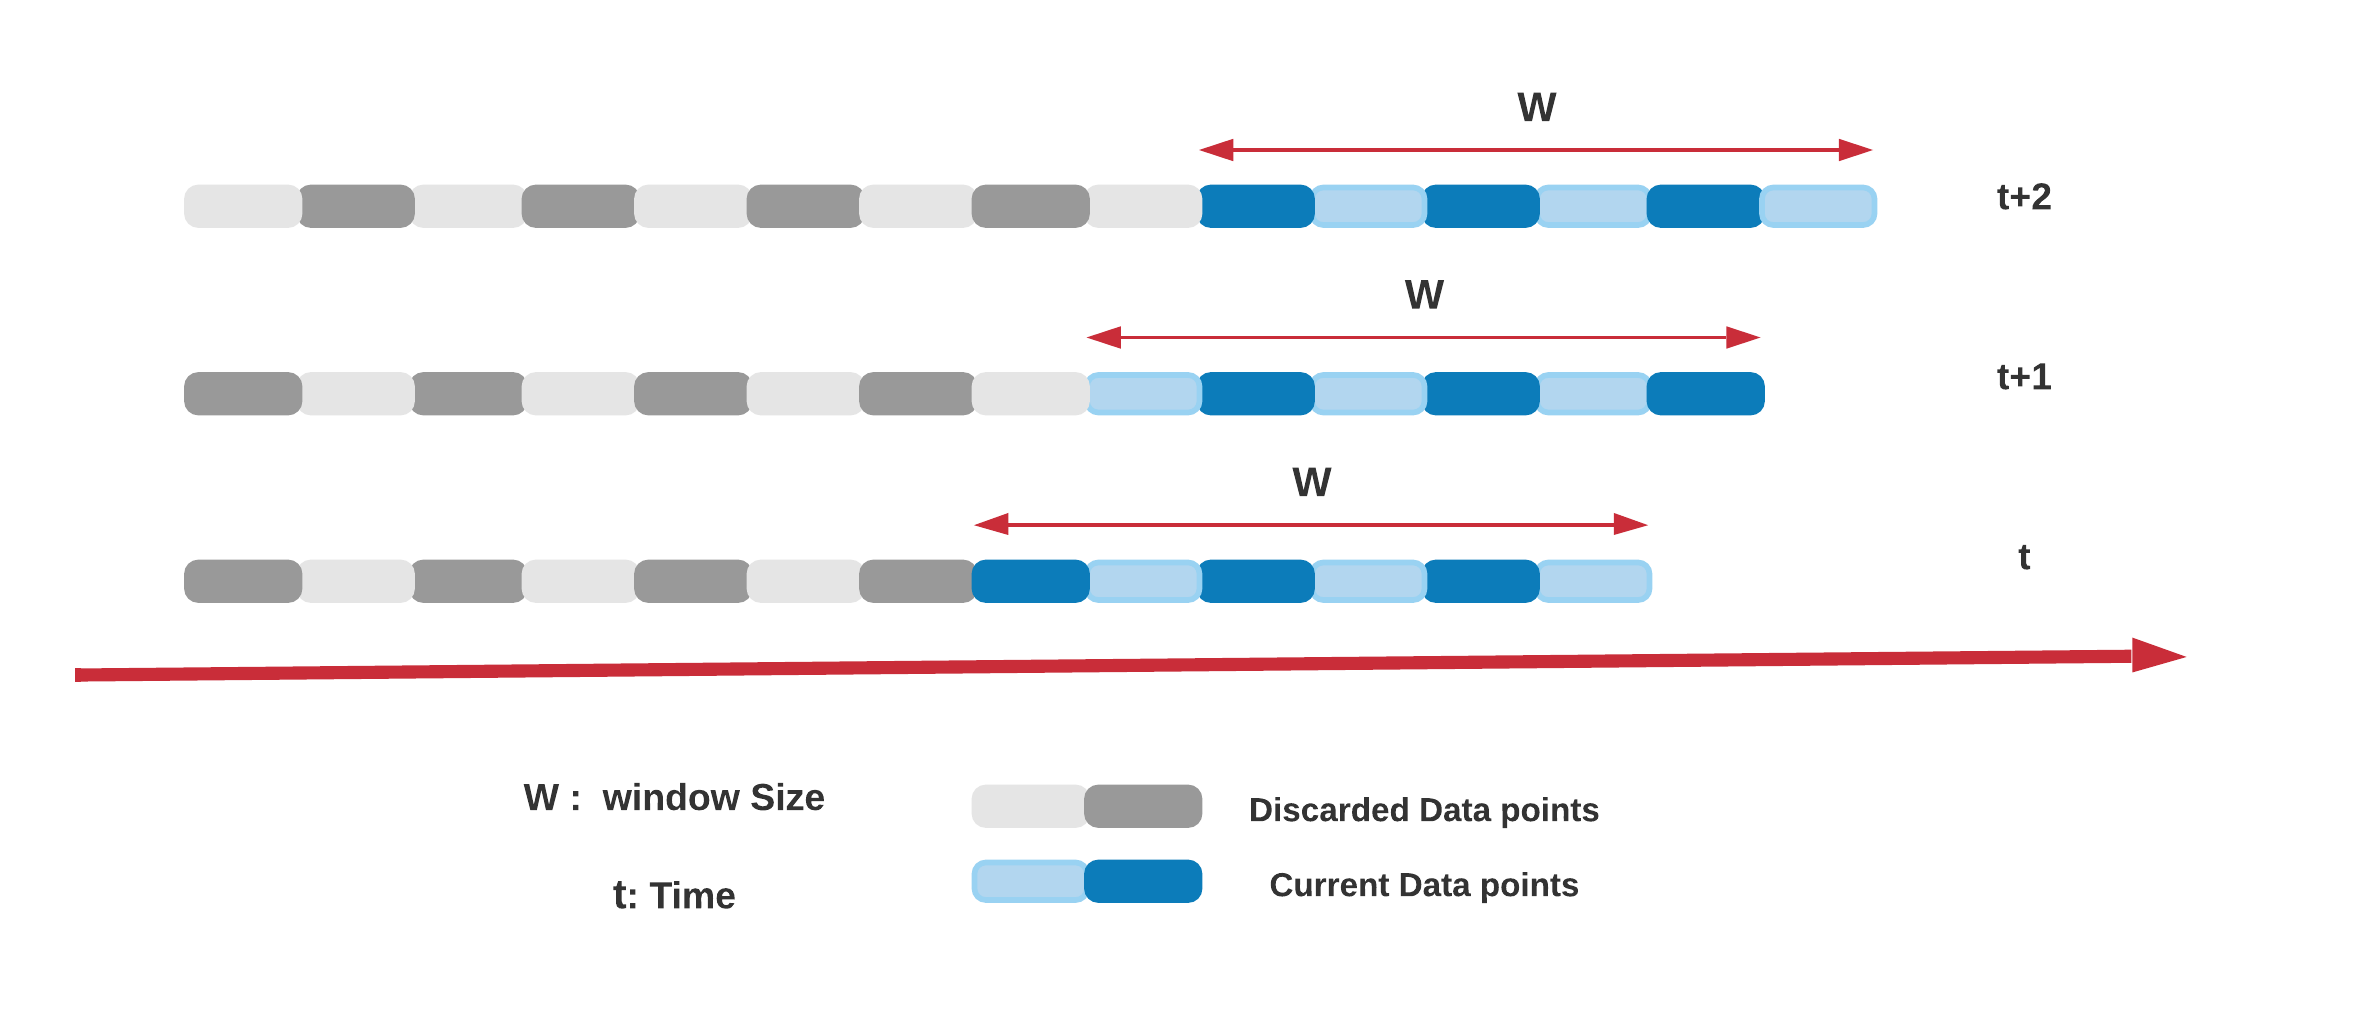
\includegraphics[width = 14cm,height = 7cm]{image/stw (2).png}
% \caption{Sliding time window model applied in this work\cite{zubarouglu2020data}}
% \label{stw}
% \end{figure}
% \cite{zubaroglu2020data}









%%%%%%%%%%%%%%%%%%%%%%%%%%%%%%%%%%%%%%%%%%%%%%%%%%%%%%%%%%%%%%%%%%%%%%%%%%%%%%%%%%





% \begin{figure}
% \centering
% 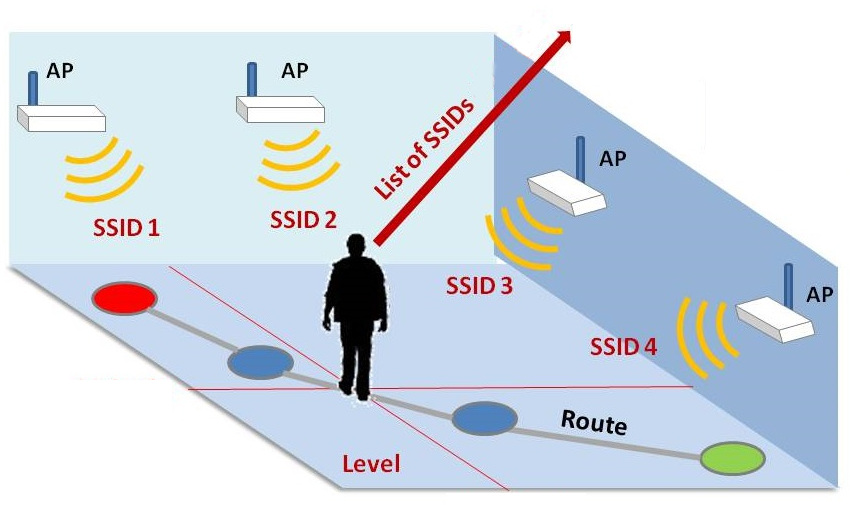
\includegraphics[width = 9cm,height = 6cm]{image/indoorp.jpg}
% \caption{Indoor positioning technique using WLAN . }
% \label{time}
% \end{figure}

%elmi


%elmi. RSSI, or “Received Signal Strength Indicator,” is a measurement of how well your device can hear a signal from an access point or router.  RSSI is a term used to measure the relative quality of a received signal to a client device, but has no absolute value. The IEEE 802.11 standard (a big book of documentation for manufacturing WiFi equipment) specifies that RSSI can be on a scale of 0 to up to 255 and that each chipset manufacturer can define their own “RSSI Max” value. Cisco, for example, uses a 0-100 scale, while Atheros uses 0-60. Since RSSI varies greatly between chipset manufacturers,

%elmi. wiki.In an IEEE 802.11 system, RSSI is the relative received signal strength in a wireless environment, in arbitrary units. RSSI is an indication of the power level being received by the receiving radio after the antenna and possible cable loss. Therefore, the greater the RSSI value, the stronger the signal. Thus, when an RSSI value is represented in a negative form (e.g. −100), the closer the value is to 0, the stronger the received signal has been. There is no standardized relationship of any particular physical parameter to the RSSI reading. The 802.11 standard does not define any relationship between RSSI value and power level in milliwatts or decibels referenced to one milliwatt (dBm). Vendors and chipset makers provide their own accuracy, granularity, and range for the actual power (measured as milliwatts or decibels) and their range of RSSI values (from 0 to RSSI maximum).[2] One subtlety of the 802.11 RSSI metric comes from how it is sampled—RSSI is acquired during only the preamble stage of receiving an 802.11 frame, not over the full frame.[3]

%Elmi. The wifi ujindoorloc can be used as an example wlan suvey data to determine the signal coverage and the density of people could be used for capacity estimation. Cisco wlan deployment guideline.




%%%%%%%%%%%%%%%%%%%%%%%%%%%%%%%%%%%%%%%%%%%%%%%%%%%%%%%%%%%%%%%%%%%%%%%%%%%%%%%%%%%%%%%%%%%%%%%






%{Scalability of Clustering Methods}
%Handling large-scale and dealing with real datasets is a key concern. High performance and large memory size cannot give accurate clustering. This section explain methods to keep the clustering computational beyond these limits.


%\subsection{Time window models for clustering}
%%---------------time window-----------------------------------------------




% \section{Positioning Technologies and Application Fields for Clustering/Spatiotemporal data clustering}

%positioning technologies
%Ecounter and Wifi examples of data.
%how ecounters work
%how wifi localization data works





% \subsection{Indoor People Counting }


% \subsection{Automatic user localization: Wi-Fi positioning system}







% \begin{table}[ht]
%     \centering
%     \caption{comparison between K-means and AP }
%     \label{comp}
%     \begin{tabular}{|c|c|c|}
%     \hline
%       & K-means & AP \\
%      \hline
%      exemplar &  generate  & actual point\\
%      \hline
%      parameters & $K$  & $S^*(penalty)$\\
%      \hline
%      algorithm & greedy search  & message passing\\
%      \hline
%     performance &  not stable & stable\\
%      \hline
%       complexity & $N * K$   & $N^2 log(N)$\\
%       \hline
     
%     \end{tabular}
    
% \end{table}


  
% \end{document}


%\subsection{Sliding Time Window for the Workflow}
%**********elmi
%To enable processing of blocking operators like average and sum over infinite data streams, windowing is commonly used in data stream processing because it limits the extent of data to a sequence of most recent elements in the data stream. Clustering algorithms are blocking since they require having all the data points to compute the clusters. Therefore, windowing is needed for data stream clustering.There are different ways of defining a window over a data stream \cite{xu2016scalable}.The window specification defines how recent stream elements are selected for windowing. When the window specification is applied on a live data stream it produces new window instances at different points in time. A window instance logically contains a set of stream elements.For example, a sliding window is specified by defining its range and stride. The range R of a sliding window specifies the length of the window while the stride S specifies the portion of the range that is evicted from the window when the window moves forward. A sliding window is specified as a tuple <R,S>, where S<R. Two common kinds of sliding windows are time-based and count-based sliding windows \cite{li2014parallel}. In time-based sliding windows R and S are defined using time intervals while in count-based sliding windows they are defined in terms of the number of elements. For example a time based sliding window with R=10min and S=2min produces window instances that cover the data in the last 10 minutes of the stream and a new window instance is created every 2 minutes. Without loss of generality, we present sliding windows using count-based sliding windows. %**********


%Generally, a clustering method for data stream is originated from a corresponding clustering method for batch data, e.g., CluStream from K-means, DenStream from DBSCAN, and STRAP from AP clustering. THIS BELONGS TO LR

%Data stream clustering finds clusters based on the flow of data, and it is different from traditional clustering \cite{toshniwal2013clustering}:

%\begin{itemize}
    % \item Traditional clustering data are static; the data stream is dynamic.
    % \item Traditional clustering datasets can be accumulated in memory, but the streaming data is enormous in size, and then it is not possible to store in memory.
    % \item traditional clustering results are fixed, but The data stream clustering results vary over time.
%\end{itemize}




%
% \begin{enumerate}
%     \item\textbf{Data collection phase:} The data collection phase involves gathering observations or measurements from sensors, cameras, or electronic devices.
    
%     \item\textbf{Data prepossessing phase:}  Real-world data is sometimes incomplete, inconsistent, and contains errors. Various techniques have evolved for handling and transforming the data into a usable format. This phase consists of data cleaning, data transformation, and aggregation stages.
    
%     \item\textbf{Data Stream Simulation Phase:} Convert the batch of data to the stream fashion. 
    
%     \item\textbf{Data Stream Clustering Phase:}Generates micro and macro clusters using a sliding time window. 
    
%     \item\textbf{Clustering Performance Evaluation Phase:} Computing cluster measurements to evaluate the quality of the clusters by the target Coefficient and indexes.
% \end{enumerate}






% \section{Data Stream Simulation}
% Since data used in this research were obtained from concluded experiments, it was essential to find a mechanism to convert the batches of data in to a data stream. The streaming data was generated from the target datasets by applying the Scikit-Multiflow package in Python for the DSAP algorithm and the DSD objects in the stream package in R for the streaming K-means algorithm. 



% \subsection{Scikit-Multiflow-based Simulation}
% The 'scikit-multiflow' framework in Python programming language is a free and open-source tool for generating data stream \cite{montiel2018scikit}. It provides multiple stream learning methods, steam generators, and evaluators, where the primary focus is on batch learning. This framework's base class is the 'StreamModel', which has abstract methods to be implemented by classes. A 'StreamModel' object interacts with other objects: ' Stream' and 'StreamEvaluator'. The 'stream' gives an endless flow of data by request, and 'StreamEvaluator' presents various tasks that are queries the stream, train, test on the incoming data, and tracks the model's performance.

% 'scikit-multiflow' needs NumPy library installed in the system. All classes are shown in Figure \ref{sci} for generating data stream. The \textit{skmultiflow} data contains data stream methods, including methods for batch-to-stream conversion and generators. In all classes, the stream is available upon request and old data points cannot be accessed at a later time. These are listed below:

% %\renewcommand\labelitemi{$\vcenter{\hbox{\tiny$\bullet$}}$}
% \begin{itemize}
%     \item {data.base\_stream.Stream:} it defines the minimum requirements of a stream and it can work along with other modules in multiflow. 
%     \item {data.DataStream:} it takes the whole data consisting of the $X$ as features and $Y$ as targets or takes them separately.
%     \item {data.FileStream:} if the data previously collected and stored in the CSV file (it just supports CSV files at this moment), it can generate streams by loading the dataset. 
%     \item {data.ConceptDriftStream:} this stream generator adds concept drift by joining several streams and giving the weight. 
%     \item {data.TemporalDataStream:} takes the dataset containing $X$ as a features and $Y$ as a targets with $time$ as a timestamps. 
% \end{itemize}

% On the other hands, as shown in Figure \ref{sci}, there are many stream generators classes for different problems listed below:
% %\renewcommand\labelitemi{$\vcenter{\hbox{\tiny$\bullet$}}$}

% \begin{itemize}
%     \item[$-$]  data.WaveformGenerator: random differentiation of some base waveforms.
%     \item[$-$]  data.SineGenerator: sine waves stream generator.
%     \item[$-$]  data.AgrawalGenerator: scaling up decision tree learners based on Agrawal model.
%     \item[$-$]  data.AnomalySineGenerator: simulate a stream with anomalies in sine waves.
%     \item[$-$]  data.LEDGenerator: seven-segment LED display stream generator.
%     \item[$-$]  data.LEDGeneratorDrift: add concept drift to the LED stream.
%     \item[$-$]  data.MixedGenerator:  data stream with abrupt concept drift and boolean noise-free.
%     \item[$-$]  data.MultilabelGenerator: the stream of samples for a multi-label problem.
%     \item[$-$]  data.RandomRBFGenerator: Random Radial Basis Function stream generator.
%     \item[$-$]  data.RandomTreeGenerator: based on a random tree that splits features at random and sets. 
%     \item[$-$]  data.RegressionGenerator: creates a regression stream.
% \end{itemize}


% \begin{figure}
% \centering
% 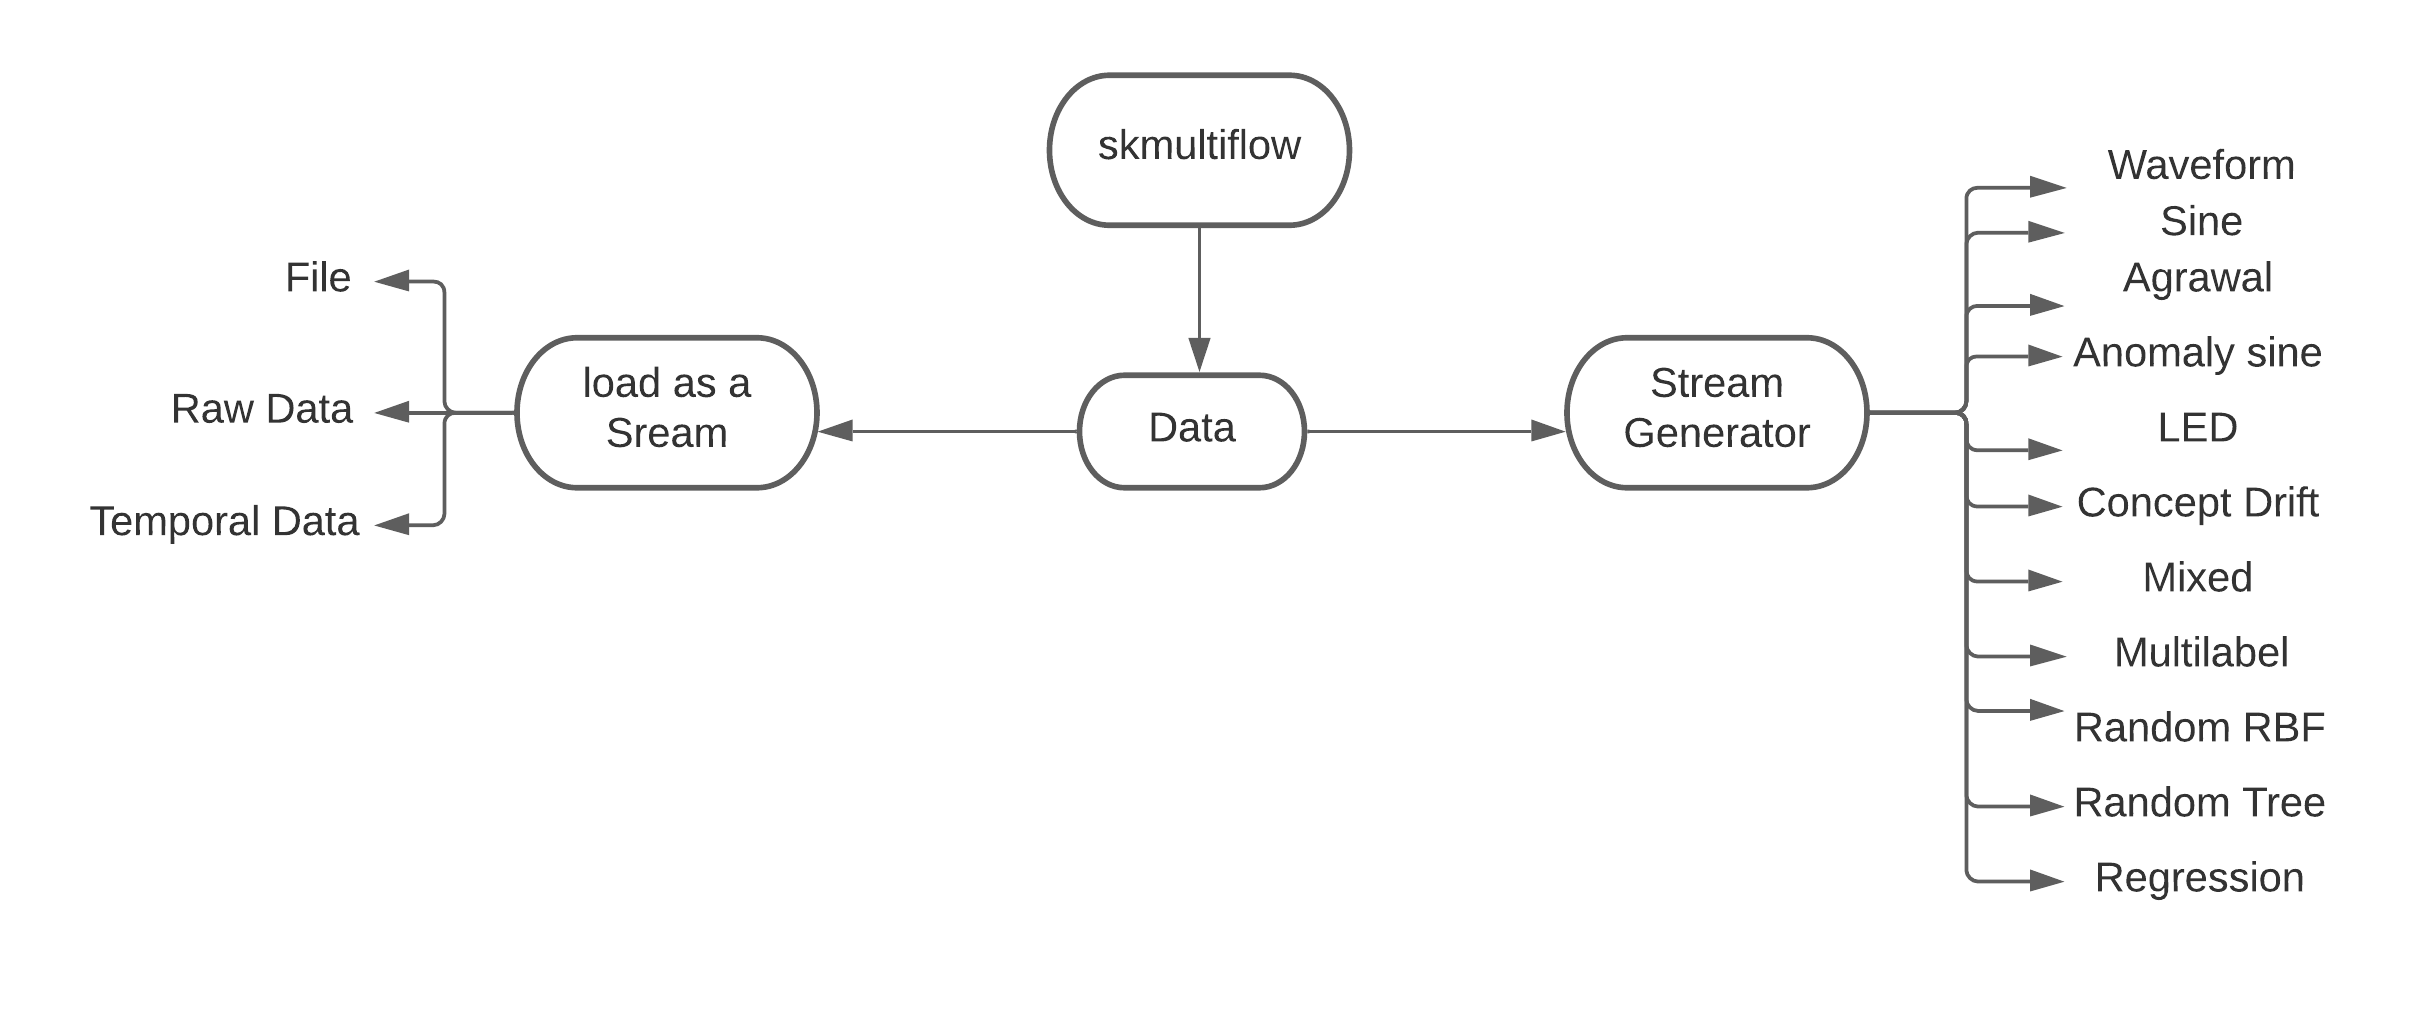
\includegraphics[width = 12cm,height = 6cm]{image/sci2.png}
% \caption{The scikit-multiflow map with multiple methods for generating data. }
% %\cite{SMF}}
% \label{sci}
% \end{figure}



% The k-means algorithm can be explained by the following 4 steps:
% Step 1: define the number of clusters (K) and randomly pick k instances as the initial cluster centroids.
% Step 2: assign all data points to the closest centroid by measuring the distance such as the Euclidean distance.

% Step 3: re-compute the centroid of each cluster by calculating mean value of all the data points in the cluster.
% Step 4: repeat steps 2 and 3 until the centroid does not change.
% https://pdfs.semanticscholar.org/1040/6a6e1319a48e731db73ed22bbde61fa42691.pdf


% \section{Comparison  Between  DSAP  and  Streaming  K-means Phase}
% The general approach of the various stream clustering algorithms that allow for the investigation of the cluster structure at different time intervals are fairly similar. They typically have two stages, online where the algorithm maintain a summary of the data as micro-clusters and next in the offline phase the summary micro-clusters are clustered to provide real insights to the data. The efficiency of these algorithms are greatly affected by the choice of the clustering algorithm used. We have introduced the DSAP algorithm for data stream clustering which is implemented based on the AP algorithm. This model is compared with the established streaming K-means algorithm introduced earlier in Chapter 2. It is known that the AP algorithm usually generates results that show that the k-means algorithm is faster than AP. However, streaming AP based algorithms has been shown to provide similar quality clusters as k-means based ones but, the results tend to be more robust.

% K-means algorithm is scalable for large datasets with different shapes and sizes and is easy to implement. The K-means algorithm is known to easily adopt to new centroids and is one of the fastest algorithms out there owing to a linear time complexity. Also, K-means guarantees convergence by trying to minimize the total sum of the square error as an objective function over the number of iterations. On the other hand, the K-means algorithm has some known drawbacks. Finding the $k$ optimum number of clusters is not a precise task that can be accurately automated. The algorithm results are a function of the initial clusters chosen and necessitate multiple runs of the algorithm with the different values to pick the most suitable clusters. During data stream clustering this process can be time consuming and make the model less accurate. The algorithm is known to have difficulties in finding the right clusters for data with varying size and density. In addition, K-means clusters centroids are affected by outliers since the mean as a statistic is sensitive to outliers. %it means outliers can drag the centroids or they may have their own centroids. 
% Lastly, even though K-means can be easily scaled to large datasets but it has difficulties to cluster high-dimension data. 


% In comparison with the K-means algorithm that needs to determine the optimal number of clusters prior by applying some methods like elbow method, the AP algorithm calculates the number of clusters internally. However, AP needs additional parameters like the damping factor and preference to be set since the model convergence is dependent on the damping parameter while the preference controls the probability of finding centroids. Due to the additional complexities in the calculation of AP it becomes prohibitively expensive to scale AP as compared to the K-means which scales linearly with the size of the dataset. The semi-supervised selection of the number of clusters in K-means limits the potential of producing large number of clusters that can sometimes be generated by the AP if it's parameters are not chosen carefully. Both these partitioning based algorithms can be evaluated based on metrics that quantify the density and spread of the clusters. 

% Affinity propagation has been shown to perform well in pattern recognition applications in the fields of computer vision and computational biology. The main advantage of AP is the robustness of its optimization. While K-means follows a greedy optimization method to find the optimum of the optimization problem, AP tackles a continues optimization problem, in which all data points are potential candidate at the beginning and clusters are gradually identified. AP does not suffer from the initialization can guarantee global optimization consistently.



%%--------------------Chapter 3------------------------
\documentclass[../UNBThesis2.tex]{subfiles}
\setlength{\parindent}{2em}
\begin{document}
\chapter{Literature Review}

short introduction describing the contents, the aim of the LR,

This Chapter 
Several data stream clustering algorithms have been implemented with the AP algorithm using different time window models. Out of all these algorithms, none of them implemented with a landmark time window model. Moreover, all these algorithms tested on synthetic and intrusion detection algorithms. There are no works that applied the stream AP algorithm on indoor localization data.


%To control which part of data is going to be processed, time window models have been proposed.
%New ideas continue evolving in data streams over time. Evolving needs updating data stream algorithms to adjust to the changes such as handle well rapid cluster evolution patterns.
%To handle and generate data in the stream mode, open-source frameworks for IoT data stream are being developed including MOA \cite{holmes2007moa}, Scikit-multiflow \cite{montiel2018scikit}, streamDM C++ \cite{bifet2017extremely} and Apache SAMOA \cite{de2013samoa}. THIS SHOULD BE MOVED TO LR

% K-medoids algorithm \cite{macqueen1967some} is a good strategy to find clusters easy and fast by randomly choosing K initial exemplars from data and assign closest data points to these exemplar as shown in figure \ref{medo}, these exemplar can be purify in the next steps. The only thing should be consider is the number of exemplars are not changeable but the algorithm maximize the size of similarities between exemplars and other objects. k-medoids algorithm requires to be run with a various random initialization to find a suitable exemplar but this works well when clusters are small.  
% \begin{figure}
% \centering
% \includegraphics[width = 11cm,height = 7cm]{image/Chapters/Chapter2/3.png}
% \caption{K-medoids greedy solution for toy dataset}
% \label{medo}%\cite{dueck2009affinity}
% \end{figure}




\section{Previous Research Work on Streaming AP }
% Using affinity propagation for streaming clustering faces two difficulties. First, AP has been implemented for batch processing but it should handle data clustering and large datasets in the online mode. The most important point to consider is AP suffers from quadratic computational complexity.
Extensive data that are continuously coming are required to store. Analyzing big datasets and extracting patterns is not possible with affinity propagation due to the time complexity issue.
One way to apply affinity propagation algorithm is using the divide and conquer approach \cite{khalilian2016data}. This approach introduced by Nittel et al.\cite{nittel2004scaling}, has mainly three steps as shown in Figure \ref{dividee}: partitioning the dataset into different chunks, then clustering each chunk and find the results, lastly, computes the results out of all chunks of data. 

\begin{figure}[!h]
    \centering
    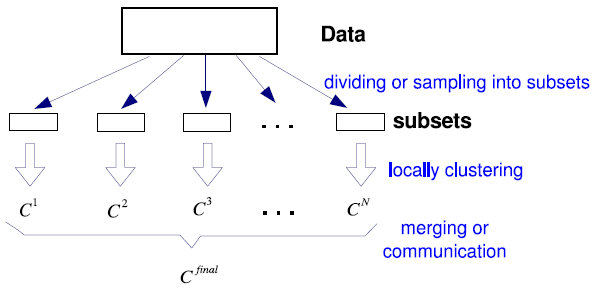
\includegraphics[width = 11 cm]{image/Chapters/Chapter3/divide.PNG}
    \caption{Divide and conquer approach to generate clustering out of big data \protect\cite{zhang2009toward}}
    \label{dividee}
\end{figure}


Our first attempt working with the extensive dataset was to implement this technique to generate data stream clustering \cite{ivarispatio}, and it was the first version of DSAP, which is presented in this thesis. However, it has a history of all data points, and the time and memory complexity are still high, and most algorithms that have this approach are unable to track the change in the trend of the data stream. 
Due to the reason above, some research has been done on AP streaming clustering and introduce new approaches.

%Elmi
% It must be emphasized that both Divide-and-Conquer and two-level schemes keep their computational load
% within reasonable limits as they only build the data model upon the users explicit request. In the rest of time, they only maintain a summary of the data, which makes them ill-suited to applications such as system monitoring where the data model has to be continuously available at all times.


There are a few algorithms are introduced based on AP algorithm for data stream clustering and they are shown in Table \ref{APCLU}. 


\begin{table}[!h]
    \centering
    \caption{Overview of data stream clustering algorithm based on AP. }
    \label{APCLU}
    \small
    \begin{tabular}{c c c c c}
    \hline
      \textbf{Algorithms} & \textbf{Year} & \textbf{ Method } & \textbf{Processing} & \textbf{Time window model}\\
     \hline \midrule
     STRAP                &   2008        &    AP             &    Online          & Sliding \\
     \hline 
     IStrAP               &   2012        &    AP             &    Online          & Sliding \\
    \hline
     APDenStream          &   2013        &    AP             &     Online-offline & Pyramidal(offline)   \\
     \hline
     SSAPStream           &   2015        &    AP             &     Online         &   Damped    \\
    \hline
     SED-Stream-AP        &   2018        &    AP             &    Online-offline   & Damped(offline)\\
     \hline
     ISTRAP               &   2018        &    AP             &   Online           & - \\
\bottomrule
    \end{tabular}
\end{table}

% The other improvement of AP to handle huge datasets was WAP or weighted AP \cite{zhang2009toward}. Under the premise of not changing the amount of passed information, this algorithm integrates the neighboring points, making the integrated points have the same clustering results with the original points.
% , zhang2013data
\begin{itemize}[leftmargin=*]

\item[]\textbf{STRAP Algorithm}

In 2008, Zhang et al. \cite{zhang2008data} proposed streaming AP called STRAP, extending affinity propagation for data stream clustering. 
This model is inspired by DBSCAN and DenStream introduced in Chapter Background. STRAP is built of several steps. 
The first step is weighted AP to handle duplicated objects without losing performance.
Second, hierarchical WAP, dealing with quadratic AP complexity and reduce it by utilizing AP on subsets of data and then utilizing Weighted AP on the exemplars obtained from subsets.
Eventually, with online clustering, STRAP extends Hierarchical WAP to deal with changes in the data distribution by updating exemplars and storing the outliers. As illustrated in Figure \ref{stmodl}, STRAP involves four main steps as follow: 


\begin{itemize}
    \item[$\bullet$] AP applied to the first bunch of data to computes the first centroids and initialized the streaming model.
    \item[$\bullet$] As the stream comes into the model, each data point $x_t$ is compared to the centroids $e_i$. This comparison is based on the Euclidean distance of $x_t$, $e_i$ with the threshold $\epsilon$, which is heuristically set, and the value is equal to the average distance between data points and centroids in the initial model. If $x_t$ is far from the nearest centroid, it goes to the reservoir. If not, $x_t$ is assigned to the ith cluster, and the STRAP will be updated accordingly. STRAP has a mechanism to forget old centroids which they have not been visited for some time and to keep them in control.
    \item[$\bullet$]  Two restart procedures have been used in STRAP. First, if the number of outliers in the reservoir exceeds the reservoir's size, the restart criterion will be triggered. Second, it is related to the distribution of the data points by applying Page-Hinkley (PH) test and detect the changing trend of data points. 
    \item[$\bullet$] If restart criterion called by either fill up the reservoir size or the PH test, model is rebuilt by launching WAP algorithm from current centroids and reservoir.
\end{itemize}

\begin{figure}
\centering
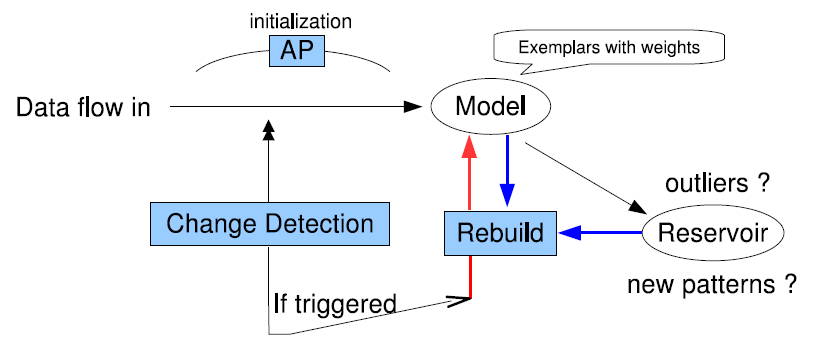
\includegraphics[width = 13 cm]{image/Chapters/Chapter3/strapmodel.PNG}
\caption{The framework of STRAP algorithm. }
\label{stmodl}
\end{figure}



% To validate a STRAP, the Intrusion Detection benchmark(KDD99) and EGEE real-world datasets are used for monitoring and discovering anomalies within a grid computing infrastructure. The result of this work is compared with DenStream, and comparatively satisfactory results are investigated. Also, computational time in this model is higher than DenStream. 


The proposed STRAP algorithm was analyzed on guaranteeing acceptable distortion loss when exemplars slightly drift from the already selected ones, with a small amount of memory and computing time. The performance of STRAP in clustering quality and efficiency is validated on the KDD’99 dataset and the URLs stream. However, STRAP improves clustering purity rather than DenStream, and computational time is also higher than the DenStream algorithm. In addition, STRAP is a model for the stream at any time, whereas DenStream only builds the model upon request. The validation on URLs stream also demonstrates that STRAP achieves very high accuracy and purity for collecting malicious URLs.




% % From APDENSTREAM:
% This algorithm can determine
% the number of clusters automatically and detect the real-time
% changes of the data stream at the same time. However, the
% clustering quality depends on the size of the sliding window.
% Meanwhile, it is not considering how the arrival time will
% affect the clustering results. The clustering effect is not
% satis factory when noises are too much




\item[]\textbf{IStrAP Algorithm}

IStrAP \cite{li2012improved} is an improved version of the STRAP algorithm to meliorating the efficiency of this algorithm. STRAP algorithm frequently applies the WAP algorithm to combine the initial clustering results with the reservoir’s data points to re-cluster in a fast manner. Clustering is sometimes ineffective due to the handling of outliers well in the reservoir. To improve the efficiency of clustering results, they introduced a method to remove outliers. This method is based on the statistical properties of the window data. The outlier refers to the abnormal behavior deviating from the normal value. Such data may be generated in emergency situations or generated when an error occurs. The process of removing outliers is consists of four steps. 
\begin{itemize}
    \item[$\bullet$]  The reservoir statistics (maximum value, minimum value, sum and average value) from received stream data are obtained.
    \item[$\bullet$] Standard deviation of data points in the reservoir are computed.
    \item[$\bullet$] The sampling parameter ($\sigma$) needs to be set. This parameter can reflect the distribution of the data in the window. The $\sigma$ value is standard deviation of the data.
    \item[$\bullet$] Outliers are being removed if they are outside of the interval equal to [Avg-$\sigma$, Avg + $\sigma$].
\end{itemize}

 

IStrAP used KDD Cup 99 dataset and used the Page-Hinkley standard test to update the clustering model. The results show that the IStrAP has higher accuracy, lower time complexity, and better adaptability for stream data over than STRAP. With this dataset, they just chose 120 data points to show the result, and the result is poorly demonstrated with the percent of accuracy and time.


\item[]\textbf{APDenStream Algorithm:}

Zhang et al. \cite{zhang2013online} proposed a data stream clustering based on AP and density methods to improve the STRAP model's accuracy and timeliness in a noisy environment. This algorithm applies two-phase clustering, online and offline approaches. The online phase detects data distribution changes of the new data points, updates the micro-cluster decay density, and generates real-time results. The offline, which invoke by the user, choose a specific time frame by applying a pyramidal time window model and gives final query results. The process of this work is depicted in Figure \ref{APden}. 


\begin{figure}[h]
\centering
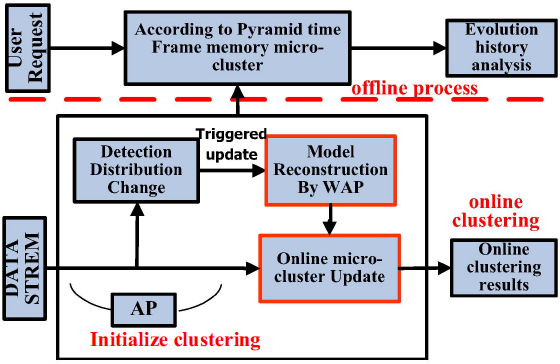
\includegraphics[width = 10 cm]{image/Chapters/Chapter3/APDenstream.PNG}
\caption{APDenStream clustering model introduced by Zhang in 2013. }
\label{APden}
\end{figure}


The overall APDenStream algorithm can be explained as follow:

\begin{itemize}
    \item[$\bullet$] AP algorithm is applied to the first $InitN$ points $P$ to initialize the online process. The first group of micro-clusters $mc$ are obtained by scanning $P$. If the micro-cluster density of the micro-cluster $mc$ is greater than the threshold $D$, it is labeled as a dense micro-cluster, and the average radius of all dense micro-clusters is being chosen as an initial radius $\epsilon$.
    
    \item[$\bullet$] The new point comes into the model, and it places to its nearest dense or sparse micro-cluster. If it cannot absorb any cluster, it goes to the reservoir. Then the model will be updated. As time passes, the number of micro-clusters and sparse micro-clusters is increased. To keep the clusters in a limited number and avoid memory issue, a dynamic online maintenance strategy is being used.  This strategy consists of two-part. One is for checking each dense micro-cluster every time period in order to determine whether to remove it. The other one is when the number of sparse micro-clusters is increasing by checking the minimum weight limit of sparse micro-clusters. 

    \item[$\bullet$] Whenever the reservoir is full, the model will rebuild, and new clusters will add to the model by applying the WAP algorithm.     
    
   \item[$\bullet$] The last step is offline processing which can master a depth-first traversal to find dense micro-clusters by the snapshot of the moment, and the more accurate micro-cluster is formed. Also, snapshot at time $t_c$ and time $t_ch$ can be found in the pyramidal time frames according to the current time $t_c$ and user-specific time range $h$. 
\end{itemize}



The experimental dataset used is KDDCUP'99, network intrusion detection with the 494020 TCP connection belongs to 23 networks. The results show that the APDenStream is more accurate than the STRAP algorithm due to the proposed summary data structure and benefited from its online elimination strategy, which maintains the potential micro-clusters in the stream in the time of removal of outlier noise point.
Also, APDenStream can remove outliers without upgrade potential noise points timely, while STRAP historical expired micro-cluster is taken into account.


% it is a good paper related to threshod, a metric for data distribution --> old DSAP with 2 threshold

\item[]\textbf{SSAPStream Algorithm:}

Atwa and Li \cite{atwa2015affinity} proposed a semi-supervised algorithm, an extended AP called SSAPStream, to handle evolving data streams over the online phase. This method is semi-supervised aims to improve the performance by learning from a combination of both labeled samples and unlabeled data. For a certain labeled data point, $x_i$ and unlabeled data point $x_j$, two possible situations may occur where the labeled data point may be associated with the unlabeled data point after ruining the AP algorithm. One is unlabeled data point $x_j$ takes the labeled point $x_i$ as a cluster centroids, and the other one is the labeled $x_i$ takes the unlabeled $x_j$ as a cluster centroids. If one of these two conditions happens, the unlabeled $x_j$ is the most similar to the label $x_i$. Then, the unlabeled $x_j$ is selected and set to the label of $x_i$. This process will repeat until all unlabeled data points finish.
They considered that the problem of data stream clustering with the damped time window model then the weight of data points $x_i$, decrease with time $t_k$ and calculated by decay function:

\begin{equation}
    w(x_i, t_k) = 2^{\lambda(t_k - t_i)}
\end{equation}

The proposed algorithm involves three main steps:
\begin{itemize}
    \item[$\bullet$] Apply AP algorithm on the first bunch of data at time $t_0$ to initialize the model.
    \item[$\bullet$] As a new data point flows into the model, it compares with the existing centroids based on the heuristic threshold; if too far from the nearest centroid, it goes to the buffer, or if it is far, the model will be updated. The threshold $\epsilon$ is set to the average distance between data points and centroids in the initial model.
    \item[$\bullet$] If a buffer is full or a change in the stream is detected, the model is rebuilt, and buffer 
    \item[$\bullet$] To prevent the number of centroids goes beyond the control, old ones should be removed. For each centroid, if not any new data point is merged, the weight of the centroid will decay gradually, and it should be deleted.
    \item[$\bullet$] In order to detect changes in the model, an exemplar variation threshold $\delta$ is introduced to determine if the ratio of data points associated with the centroids is big enough. If the centroid that exceeds $\delta$ is seen as a new cluster centroid. Then, the number of centroids is counted, and the ratio of different these centroids is compared with the new threshold $\phi$. If the ratio of different centroids is larger than the threshold $\phi$, many centroids are varied in the ratio of data items, then the model should be updated.
\end{itemize}


To evaluate the effectiveness and efficiency of the algorithm, two real and two synthetic datasets are used. Two real datasets are KDDCUP99 and URLs. KDDCUP99 contains a range of TCP connection records of LAN network traffic. The URLs dataset is used to predict malicious URLs from good ones.
The SSAPStream algorithm results are compared with the StreamKM++, DenStream, CluStream, and STrap. The output shows that these algorithms have advantages over other algorithms in memory usage except the StreamKM++. 
To set threshold parameters, they suggested finding the data distribution changes that are not easy for many streaming data. 


\item[]\textbf{SED-Stream-AP Algorithm:}


The other stream clustering approach based on the online and offline process is called SED-Stream-AP \cite{sunmood2018evolution}, Based on the evolution-based clustering of SED-Stream, which is able to support the evolution of clustering such as appearance, disappearance, self-evolution, merge and split. The. In the online phase, SED-Stream-AP is able to detect evolving clustering structures, which are cluster appearance, disappearance, self-evolution, merge, and split. During the offline phase, the AP algorithm is adopted to find the final clustering results. The algorithm flowchart is illustrated in Figure \ref{sed}.

\begin{figure}
\centering
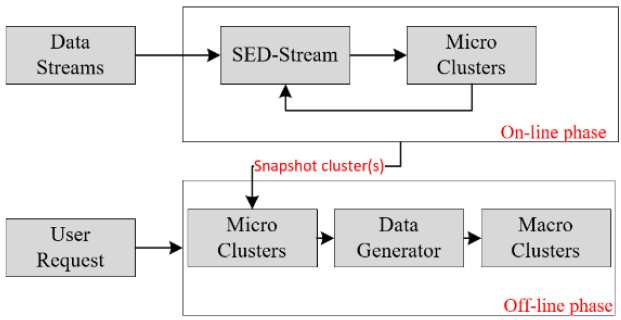
\includegraphics[width =10 cm]{image/Chapters/Chapter3/sed.PNG}
\caption{The framework of SED-Stream-AP algorithm.}
\label{sed}
\end{figure}


The online phase of the SED-Stream-AP algorithm is formed with different steps. First, when a new data point flows into the model, existing clusters in the SED-Stream-AP fade by decay function. Then, based on the splitting and merging features, the algorithm splits and merges the potential clusters if they are needed. Next, if any new cluster appears, it is considered as an active cluster. Lastly, the incoming data point is assigned to the closest cluster.  Otherwise, it creates its 1-element cluster. Specifically, cluster split is based on the distribution of dimension values summarized by the cluster’s histogram.
If a statistically significant valley is found between two peaks in the histogram’s value along dimensions, the cluster splits. 

The offline phase operates with the user request and consists of three steps. 
\begin{itemize}
    \item[$\bullet$] Retrieves micro-clusters have been obtained from the online phase by using FCH (Fading Cluster Structure with Histogram), a data structure that keeps representations of all the micro-clusters.
    \item[$\bullet$] Generates new data points only selected dimension from the online phase using cluster representations. The number of data points to be generated is defined based on the weight of the online phase micro-clusters
    \item[$\bullet$] calculates macro-clusters using the affinity-propagation clustering algorithm.
\end{itemize}


The SED-Stream-AP algorithm is evaluated by six different datasets, which are KDDCUP'99, forest covertype, Statlog, breast cancer Wisconsin, electricity, and synthetic datasets. 



\item[]\textbf{ISTRAP Algorithm:}

Another work on AP streaming clustering is ISTRAP \cite{sui2018dynamic}. ISTRAP is an improved model of STRAP which has been introduced in 2018. This model which inherits advantages of STRAP algorithm, gains better performance in terms of cluster evolution. This algorithm can detects three types of evolution patterns: emergence, disappearance, and re-occurrence which STRAP can handle the first one and the next two types are implemented in this work. Cluster emergence refers to the occurrence of a new cluster at time $t$. Cluster disappearance refers to the existing cluster that is not visited by the recently arrived data
points. Disappeared clusters need to be removed from the model. Cluster re-occurrence defines where a previously disappeared cluster recurs at time $t$.

For this algorithm, two reservoirs are introduced: one is the for saving the outliers (emergence) and the second one is for storing inactive clusters (re-occurence). Also, ISTRAP defines the clusters into two states, active and inactive, at each timestamp. Active state means that the cluster is still valid at current timestamp because at least one data point is assigned to it during a time interval. Inactive state indicates the corresponding clusters are expired because they are out of recent data point which representation for any pattern of the data.
the framework of the ISTRAP algorithm is illustrated in figure \ref{istrap} which is described as below:

\begin{figure}
\centering
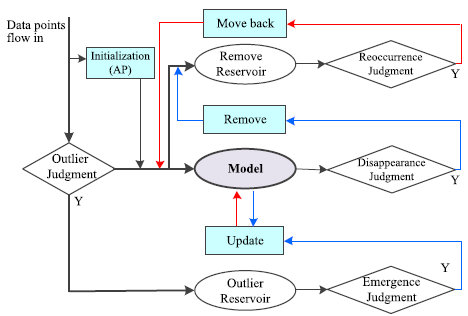
\includegraphics[width =10 cm]{image/Chapters/Chapter3/istrap1.PNG}
\caption{The framework of ISTRAP algorithm.}
\label{istrap}
\end{figure}

\begin{itemize}
    \item[$\bullet$] First, initial exemplars are obtained by applying the AP algorithm on the first bunch of data.
    \item[$\bullet$] As the stream flows in, each data point will go the outlier judgment step, and the minimum distance of the data point from the exemplar compares with the threshold. If it is less than the threshold, it will assign to the nearest exemplar; otherwise, it goes to the reservoir.
    \item[$\bullet$] All clusters in remove reservoir are checked if they re-occur, then recurrent clusters will be moved back into the model
    \item[$\bullet$] The emergence criterion is triggered if new clusters need to be obtained. So, from the outlier reservoir, the model will be rebuilt by the WAP algorithm.
    \item[$\bullet$] The model will check all active clusters if they are still active or not. The inactive clusters will be removed and goes to the removed reservoir.
\end{itemize}

The clustering quality of this algorithm depends on mostly four parameters that need to be chosen carefully, such as $\delta$, $\alpha$, $\beta$, $\lambda$. The effect of three forms of evolution by controlling the number of outliers or $\delta$. The threshold for emergence detection is defined by $\alpha$, and it affects the stability and processing time of the algorithm. The maximal duration tolerance or $\beta$ means an active cluster is not visited by new data points. Larger $\beta$ means less possibility that clusters are inactive. The last parameter $\lambda$ represents the minimum number of data points assigned if recurrent clusters have to be sent to the model, and if $\lambda$ is small, it means more recurrent clusters are detected. 

Four Real datasets and two artificial numerical datasets are applied to evaluate this algorithm. The real-world data stream,  MNIST, contains handwritten digits from 0 to 9 and is used to test the performance of the ISTRAP. In the end, the results compared with the STRAP algorithm and find out that STRAP is unable to detect re-occurrence. However, ISTRAP has very powerful effectiveness in tracking the re-occurrence of the with a delay.







% \section{K-means Stream Clustering}
% For scalable and low-complexity way of transferring data from network to the mobile phones \ref{cramariuc2016clustering}.




%%%%##########  FOR now -- uncomment 
% \section{Data Stream Clustering}

% To perform data stream clustering to access and see the data over the time many data stream clustering algorithm have been introduce.
% CluStream \cite{chen2007density} is online and offline framework for clustering dynamic streaming data. This algorithm uses Pyramidal time window that allow micro-clusters to split and merge over time. Online phase, is sampling process of the $k$ desired clusters and this $k$ clusters are emitted at chosen time intervals, through some off-line clustering method.


% A common baseline algorithm for streaming clustering, is streaming k-Means \cite{ailon2009streaming, braverman2011streaming} uses its update process from the Lloyd algorithm. However, similar to CluStream, micro-clusters is maintained in online phase, to be further clustered in an off-line step. Similar to K-means, streaming K-means has the same process for assigning incoming data points to the nearest representative cluster. The value for having $k$ number of cluster is not available, and this can be done with some sort of inter-cluster similarity or intra-cluster dissimilarity metric. the main drawback of streaming k-Means is that it is highly dependent on the input order of the data stream.

\end{itemize}

%any streaming algo for indoor

\todo[inline]{research premise}
There First group is partitioning data stream clustering algorithm which they are listed in Table \ref{landmarkwin}. As far as we had research, there is not any research work present with affinity propagation used landmark time window model.

There is no paper related to occupant behaviour(stair usage) + stream clustering???
There is no paper related to ecounter(sensors) + clustering as well as stream clustering????

paper related to people counter+ clustering ????

Several data stream clustering algorithms have been implemented with the AP algorithm using different time window models. Out of all these algorithms, none of them implemented with a landmark time window model. Moreover, all these algorithms tested on synthetic and intrusion detection algorithms. There are few works that applied the AP algorithm on indoor localization data. _>> to be used for conclusions


% \section{occupancy}
%\section{Latest Development in Indoor Localization }

PAPER'S BELOW SHOULD BE MOVED TO THE PREVIOUS METHODS


The people’s counting is a very important topic to design any system for behavioral analysis. It is used to measure and manage people’s behaviour within area.

Using stairs and monitor human activity in the building is one scenario for indoor localization and behaviour analysis.


%Carbonare et al. \cite{carbonare2018clustering} uses clustering method to investigate the occupant behaviour and their pattern in residential buildings. Two clustering method have been used: Whole time series and feature clustering with the K-means and these features are window opening and indoor temperature. The results show that feature selection has a better output than time series clustering. ?????
   


%There are many works dealing with the indoor localization problem by using WLAN-based techniques.
Clustering method could efficiently reduce computational complexity and memory requirements in large fingerprinting localization data to train ANN model. K-means clustering algorithm is one of these algorithm which is easy to implement with low time complexity. However, this algorithm is starts with an initial guess as a number of clusters, which is in the condition of close to the true solution to avoid local minima. Selection of such a starting point is not easy. Also, it would affect the location accuracy performance \cite{das2007automatic, ding2013fingerprinting}.

Genming et al. \cite{ding2013fingerprinting} introduces a fingerprinting-based localization algorithm using affinity propagation in conjunction with neural network. 
This model consists of two stage offline and online. The offline stage applies clustering and ANN training on the data. First,  a set of RSS from N available access point is collected and stored in the database. AP clustering algorithm is used in this part to to reduce the computation cost and memory of the system and partitions the reference points into different clusters represents by centroids. After clustering, the training of artificial neural network is carried out for each cluster.
The online stage, the unknown location is obtained by in two steps. First, by applying pattern matching to calculate the similarity between the new collected signal and cluster centroids and then choose sets of best match clusters for the next ANN localization phase.

Xuke et al. \cite{hu2015improving} proposes an improved WiFi fingerprinting positioning algorithm called WKNN-SAP. First, a new fingerprint distance estimation using RSS distances and access points similarities is used. Then, semi-supervised AP clustering algorithm is applied to find isolated points and remove them to have a reasonable clustering output and eliminate some outliers.

On the other hand, they applied K-means algorithm to compared both clustering results to improve the localization accuracy. and they figured out that while AP outperforms Kmeans in both the accuracy improvement and stability and this is because AP algorithm is less affected by the clustering number. Moreover, proposed fingerprint distance model can better adapt to the indoor environment with distinct access points.

%Existing stream clustering algorithms often have issues regarding asymptotic scalability [3], dimensionality limits [4] and robustness to noise





Lee et al. \cite{carraher2016random} introduces streamingRPHash is motivated by
a particularly difficult case in Nearest Neighbor, a method for clustering high-dimensional data streams to solve the other clustering problem on streaming data by applying two real world dataset, ujIIndoorLoc and ‘Human Activity Recognition datasets.
For UjIIndoorLoc data, based on the 520 of signal strength intensity, building ID is used as the target variable which has three possible values related to each building.
Human Activity Recognition datasets has 561 attributes representing time and frequency domain variables.
the result of the proposed algorithm is compared with the streaming K-means, and DSt algorithms and it shows that their proposed algorithm and streaming K-means have the same results in term of run-time and memory requirement but with increase the dimension, streamingRPHash has a better result.



To the best of our knowledge, streaming AP models have not yet been applied for any people counting data streams.  

 STILL TO FIND OUT THE RESEARCH PREMISES: WHY ARE POUR APPROACH MOST SUITABALE FOR CLUSTERING INDOORL LOCATION DATA STREAMS..


Data stream affinity propagation algorithm has been chosen for indoor localization data in this research work. For this algorithm, every data point is an exemplar, and it means they have equal importance and there is no prior reason for preferring one observation over another one. Also, the AP algorithm does not require the number of clusters as an input which makes our work more robust, especially if it uses for the cloud side. AP's main issue is the computation efficiency that we make it possible by applying the time window model and making it a stream. This algorithm is applied in many scientific research and different datasets such as intrusion detection, energy, gene expression, psychology, business, physical science, social science, etc. However, to the best of our knowledge AP model has not yet been applied for any people counting data and streaming AP for any indoor localization dataset.

K-means algorithm is one of the most common methods for clustering distance-based objects that we have applied for our data. However, this method is less effective, or even inapplicable, for the application we used. For example, K-means results find cluster centroids between locations which does not make sense for our interpretation. 


%  affinity propagation can be used to cluster objects measured on non‐distance‐based similarity measures that arise in psychology, such as those obtained from stimulus recognition or paired comparison tasks (see, for example, Hubert, Arabie, & Meulman,






\end{document}
%%-----------------Chapter 4---------------------------
% \documentclass[../UNBThesis2.tex]{subfiles}
% \usepackage{adjustbox/}
% \usepackage{array,booktabs}
\setlength{\parindent}{2em}
% \begin{document}

\chapter{Data Stream Affinity Propagation}
%This chapter introduces a conceptual framework capable to process data stream clustering using a sliding time window model. 

%This Chapter introduces the Data Stream Affinity Propagation (DSAP) algorithm as a novel data stream clustering algorithm that uses the sliding time window model for data analysis. 

%While most of the current data stream algorithms can process a specific form of data, our proposed DSAP is capable of handling any form of streaming data. In addition, its ability to extract summary information from a large number of internet of things (IoT) sensors made the model more powerful compare to other algorithms. 

This Chapter describes the research methodology adopted for developing, implementing, and evaluating the proposed Data Stream Affinity Propagation (DSAP) algorithm using the landmark time window model. This algorithm is based on previous research work where the online-offline clustering phases have been suggested to overcome the clustering limitations such as detecting abrupt and gradual changes as soon as they occur, and distinguishing drift from noise. Figure \ref{wrk1} provides an overview of the methodology which can be described as follows:

%We introduce the algorithm of DSAP and compare it with the established streaming K-means algorithm. The sliding time window model is used in a clustering data stream in this work to handle the recent data. The three main phases that a stream clustering algorithm employs are as follow. They are depicted in 

\begin{itemize}
    \item\textbf{DSAP Clustering Phase:} computes micro-clusters using a landmark time window model to harvest data streams.  It also computes macro-clusters by re-clustering all the centroids of the micro-clusters found in each time window. The goal is to discover hidden dense clusters structures from indoor localization data streams.
    
    \item\textbf{Intrinsic Clustering Validation Phase}: assesses the quality of the clustering results when there is no ground true label of data. The selected metrics are silhouette index, Caliński-Harabasz index, and Davies-Bouldin index. The focus is to assess between-clusters dispersion and inter-cluster dispersion for all clusters. 
    
    
    
 \begin{figure}[h!]
\centering
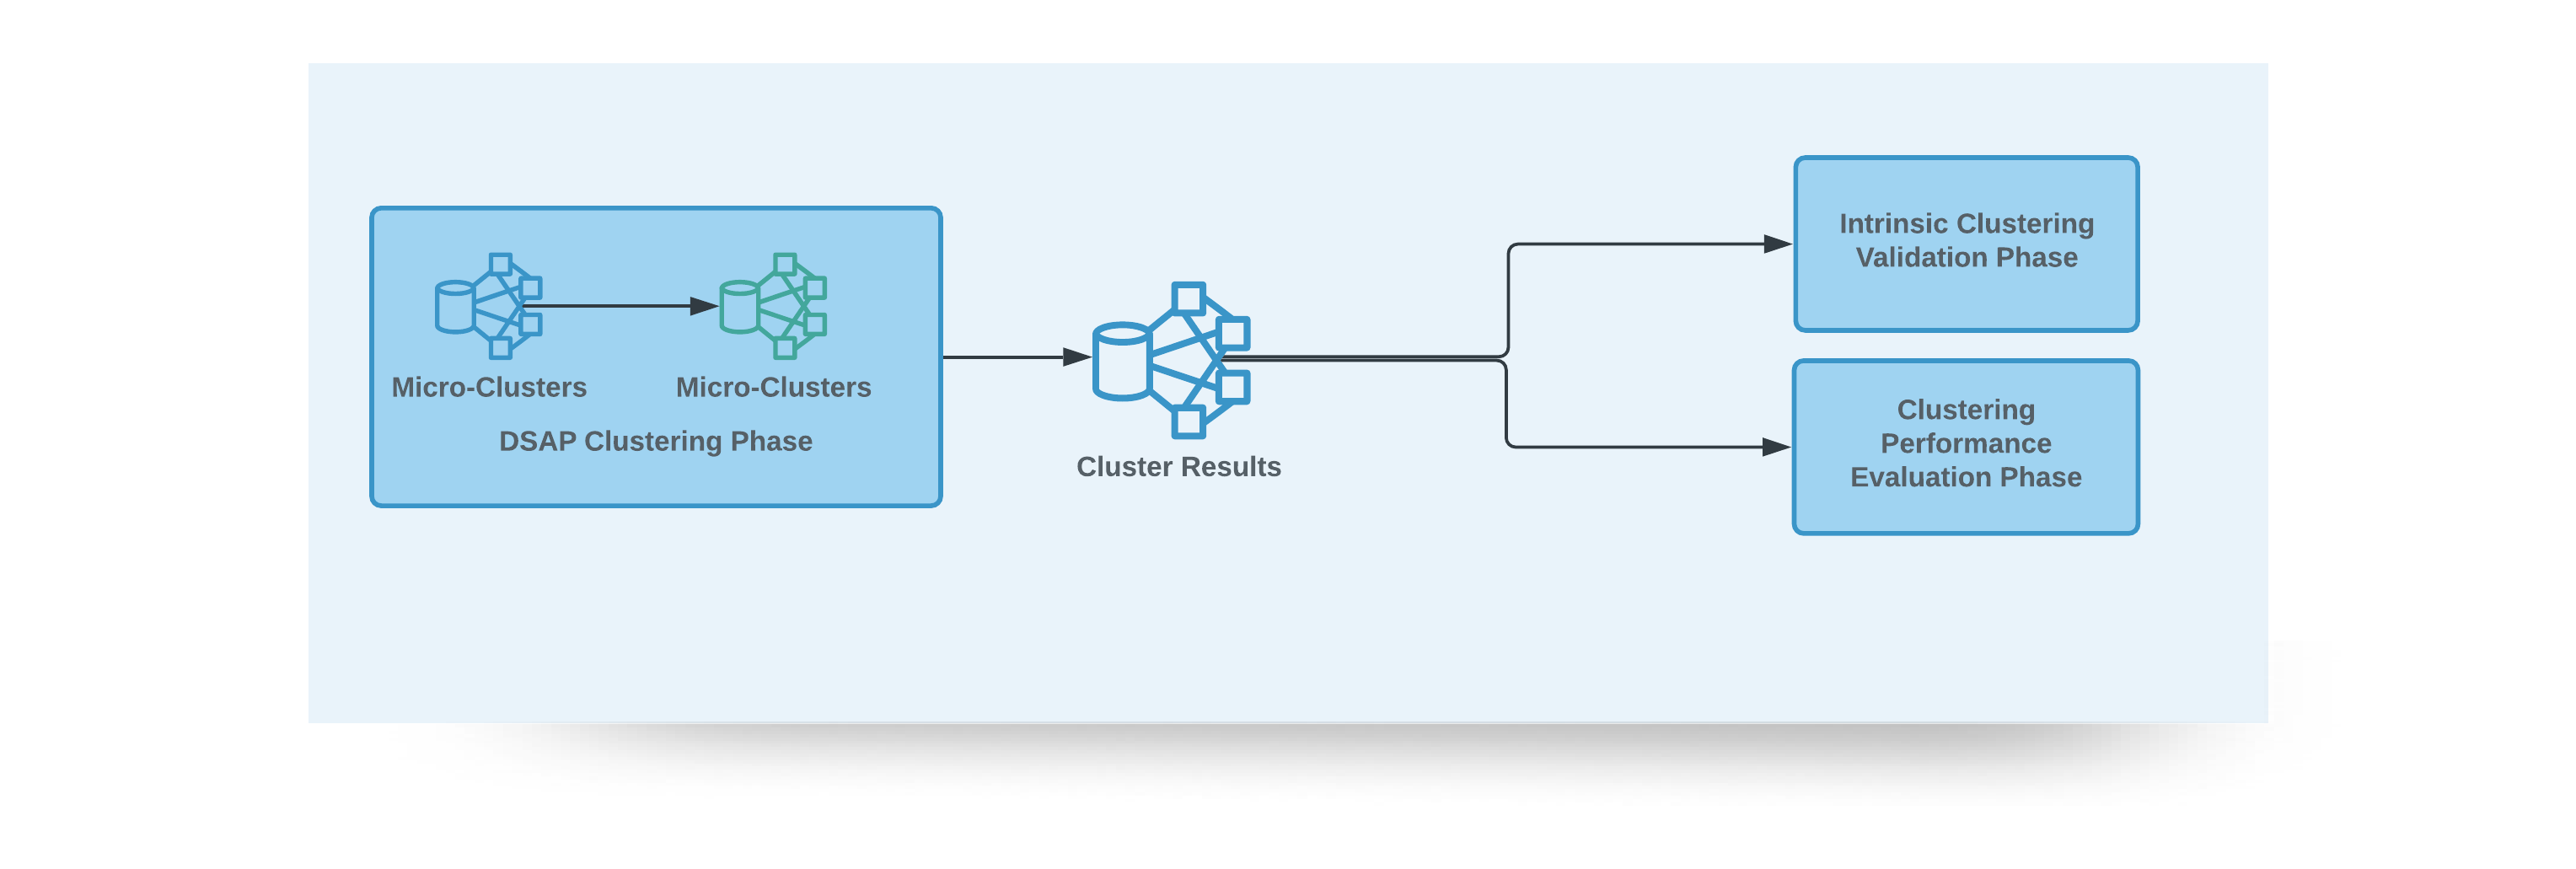
\includegraphics[width = 16 cm]{image/Chapters/Chapter4/phaseDiagram.png} %Blank diagram6
\caption{Overview of the DSAP Phases}
\label{wrk1}
\end{figure}
   
    \item\textbf{Clustering Performance Evaluation Phase:} estimates the efficiency of the DSAP algorithm using the time and space complexity metrics. The aim is to find the right balance between memory consumption and the speed of execution for the DSAP algorithm.
    
   % \item\textbf{Comparison between DSAP and streaming K-means Phase}: The aim is to demonstrate the relevance of the proposed DSAP approach compared to streaming K-means algorithm.
    
\end{itemize}




These phases are described in more detail in the following sections. First, The DSAP clustering phase, with two phases, online micro-cluster and offline macro-cluster, is introduced. Then, the clustering validation and performance evaluation phases are explained.



%%%%%%%%%%%%%%%%%%%%%%%%%%%%%%%%%%%%


%Data stream micro-clustering phase requires a process for saving the summary statistics of a data stream in a fast manner. The online part has a responsibility to maintain the micro clusters of the stream objects. The offline phase uses the last stage summary statistics to provide the user with a fast understanding of the clusters whenever the user submits the request \cite{xu2017fat}.The offline component uses online micro-clustering to find macro clusters.In the next section, first, the sliding time window used in this work will introduce, and then the DSAP data stream clustering will be proposed. In the following, the streaming K-means will be discussed. 



\section{The DSAP Clustering Phase}
The DSAP algorithm is based on the online and offline clustering phases. The online micro-cluster phase detects newly arriving data points and updates the historical clusters accordingly. The offline macro-cluster phase generates summary clusters from the centroids of the micro-clusters at the end of the data stream. 




\subsection{Online Micro-Cluster Phase}

%The online clustering phase initializes a set of micro-clusters with centroids and subsequently analyzes the latest data stream by applying the landmark time window model in a continuous manner that gives updated micro-clusters. (THIS PARAGRAPH DOES NOT MAKE SENSE)
 The online micro-cluster phase initializes by receiving data streams as a continuous sequence of data points that are harvested using the landmark time window model. Therefore, the specifications for creating a landmark time window are its start time and landmark duration $L$ with $\Omega$ data points, where
 $x_i$ is the $i^{th}$ data point in the $j^{th}$ window ($W_j$) in such a way that
 
  \begin{equation}
W_j = \begin{cases}
    0 \quad \phantom{\infty}\text{: if}\,\, i < \Omega  \\
    x_{i+(j-1)*\Omega} \quad \phantom{}  \text{, where $i$=1,2,...,$\Omega$}\,\, :Otherwise  \label{landmarkcal}
      \end{cases}
    \end{equation} 
 %$x_i$ number of arriving data points should follow the following rules
% will as shown in Equation \ref{landmarkcal}. 
 
Data points in the same landmark window are treated as equally important. In practice, the landmark duration can be defined by using a landmark time interval (e.g. every hour) or by a landmark event (e.g. every 100 data points). Every time a new window is created, all the data points from the previous windows are discarded as illustrated in Figure \ref{land}. In this thesis, the landmark time interval was selected for clustering localization data streams as for these applications only the summary of the system state within a particular window was required. This window model is suitable for our clustering process, since we are interested in the most recent data within the time frame. All data points within the window have the same weights, which make appropriate for comparing hourly, daily, or monthly summary comparisons. 

%\todo[inline]{do we have a reason to select the landmark time interval???}



   \begin{figure}[!h]
    \centering
    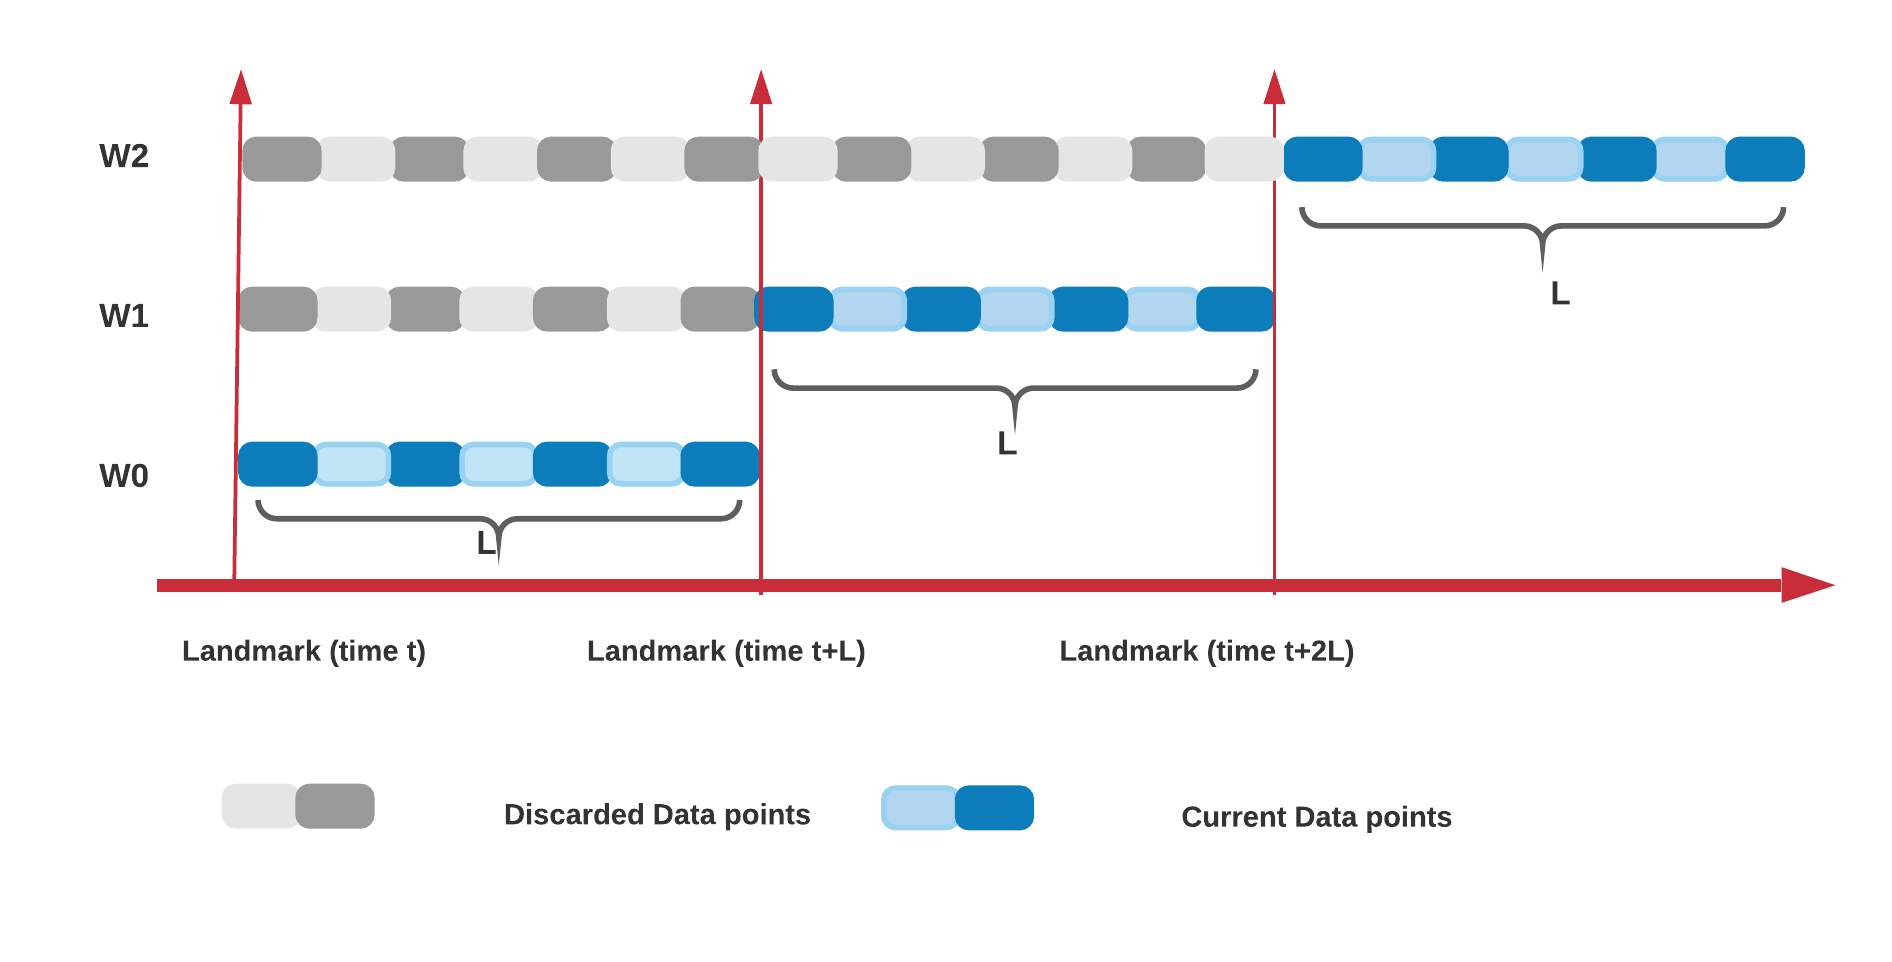
\includegraphics[width = 11 cm]{image/Chapters/Chapter4/LANDMARK-2.png}
    \caption{Landmark time window model }
    \label{land}
    \end{figure}
 
This online micro-cluster phase consists of three major steps: initialization, comparison, and activateAP and update $\epsilon_{W_j}$. %The tasks performed during these three steps are implemented in Algorithm 5.1 described in the next Chapter.

%If the next starting time is not available, we calculate the first time after the last time of the data in the window  [0][0].    
    % \[    \left [  s_{1} =\left ( E{1},N_{1},\sigma_{1},t{1} \right )  \right ], \left [ s_{2} = \left ( E_{2},N_{2},\sigma 2,t{1} \right ) \right ],\]
    % \[
    % ...,\left [ s_{i} = \left ( E_{i},N_{i},\sigma i,t{i} \right ) \right ] \] 


% Nei. Adding the last two phases, limited by free version.
  
    
    % Monica. Data Streaming with AP (STRAP): how the DSAP steps differ from STRAP steps???
    % Monica    
% 1. it does not have micro-macro clustering
% 2. using the slide time window (time duration) different from STRAP
    % Nei. Differences. 
    % 1. STRAP does not have micro-macro clustering phases. They claim that this makes the algorithm better than some of the others like Denstream since Strap always has an updated valid model while the others only maintain summaries(micro clusters). DSAP maintains the time history of data as micro clusters and updates the model (macro phase with time weighted micro clusters) periodically/user invoked like denstream.  
    % 2. DSAP employs Time windows on the data. The time dependence in STRAP comes only after the clustering/update stage where the older clusters are removed i.
    
    % 3. Model update. Once the reservoir is filled the AP restarts. But methodology to update the model are different. STRAP employs weighted clusters with some decay while DSAP adds an additional AP step so that only the cluster centroids are compared to update the prime centroids removing the need for a weights which would have added another potential variable. The decay of the centroids too will be different(currently not part of DSAP as you rightly pointed out in the last meting. I am leaning towards using the mechanism used by DBStream and SCluStream) 
    



% Monica. repository is equal to the TW, that is a problem....
% Nei: Old flowchart might have been confusing. The new version should fix this. The repository gets filled by points in any new time window that does not belong to any existing prime centroids. The repository consists of points over multiple time windows but within a reasonable time period that can be user defined and each point has a time dependent weight(still deciding) attached to it. This resolves the issue of older points corrupting the new model.

% Monica
% \begin{emph}
% {
% This section describes the StrAP algorithm, extending AP to Data Streaming,
% involving four main steps (Alg. 1):
% 1. The first bunch of data is used by ∗AP to compute the first exemplars and
% initialize the stream model. %Nei: The step names are similar hence it might have been confusing. The DSAP is inspired from Strap hence I kept the step names the same/similar for easy understanding. Initialization step. DSAP and Strap are the same. Ours is the first window from the sliding time window while Strap uses a bunch of points to find initial clusters.
% 2. As the stream flows in, each data item is compared to the exemplars; if too far from the nearest exemplar, it is put in the reservoir, otherwise the stream model is updated accordingly (section 3.1). % Nei: Update. This is similar between Strap and Dsap.
% 3. The restart criterion is triggered if the number of outliers exceeds the reservoir size, or upon a change point detection in the data distribution (section 3.2).% Nei: This step is called Restart criterion/Model rebuilding by Strap. We are calling this Activate AP step. The update criteria is different between Dsap and Strap. Change detection(data distribution change) not yet implemented in DSAP. 
% 4. If it is triggered, the stream model is rebuilt from the current exemplars and the reservoir, using ∗AP again (section 3.3). % Nei: Activate AP step. The stream model is rebuilt from the current exemplars(prime centroids) and reservoir centroids. This is different from Strap Model rebuilding phase.
% }
% \end{emph}

\begin{itemize}[leftmargin=*]
  

\item[]\textbf{Initialization}


The data stream is ingested in a windowed manner using the landmark time window model $W_0, W_1, ..W_j, ..,W_N $, where each window $W_j$ contains $\Omega$ data points and $L$ is defined as the time interval of window $W_j = [x_1,x_2...,x_i,..x_{\Omega}]$.

The clustering process is initiated by assigning the first sequence of data points from a data stream to the initial landmark time window $W_0$ as illustrated in Figure \ref{land}. The landmark time interval is a-priori determined based on user requirements, data rate, and expected latency of the expected data streams. For example, if high latency is expected in harvesting the data points, a long duration for the time intervals is advised. In contrast, in processing data from high rate streams, short time intervals will improve the clustering process. 

The AP algorithm is applied to the all data points belonging to the first time window $W_0$ for computing the initial micro-clusters and their respective centroids $C_m = C_{m_1}, C_{m_2},..C_{m_q}$. 

The micro-cluster centroids produced by the DSAP algorithm are represented as sequence of tuples:
    
    \[    \left [  s_{1} =\left ( C_{m_1},N_{1},t_{1} \right )  \right ], \left [ s_{2} = \left ( C_{m_2},N_{2}, t_{2} \right ) \right ],\]
    \[...,\left [ s_q = \left ( C_{m_q}, N_q, t_{q} \right ) \right ] \]  
    where
    \begin{itemize}
        \item[--] $C_{m_q}$ is the centroid of a micro-cluster $q$,
        \item[--] $N_q$ is the number of data points assigned to the cluster $q$, and
        \item[--] $t_{q}$ is the last timestamp assigned to the micro-cluster $q$.
    \end{itemize}

All data points within the initial landmark time window are considered as a potential exemplar until a robust set of centroids and their respective micro-clusters are found by computing the four AP matrices, i.e. similarity matrix, responsibility matrix, availability matrix and criterion matrix. The hyperparameters such as the preference parameter, the damping factor, the maximum number of iterations, and the convergence iteration are also set up during this phase. Their values will be constant throughout all the landmark time windows in the online micro-cluster phase.

A new hyperparameter $\epsilon_{W_j}$ is introduced in the DSAP algorithm for incrementally computing the clusters as time passes by, and as a result, allowing the analysis to take into account the changes of recurrently occurring clusters. For the initial time window $W_0$, an intra-cluster distance matrix is calculated between all data points and their respective centroids of each cluster using the Euclidean distance function. The mean of all these intra-cluster distances gives the initial value of the $\epsilon_{W_0}$ threshold that will be used in the next step.

The outputs of the initialization step are a set of micro-clusters centroids ($C_m$) and an initial $\epsilon_{W_0}$.


   
    
    % Monica. after you created a sequence of new TW with the same duration using a fixed time interval, and then for each TW you collect the data tuples, and compute the micro-cluster. 
    
    
    % The window is defined as a weight function of two variables, the time interval $t_i$ and the current time $t$.
    
    % \begin{equation*} W(t-t_{i}) = \begin{cases} 1, & \text {if }~t-t_{i} \le D \\ 0, & \text {if }~t-t_{i} > D \end{cases}\end{equation*}

    % As time passes, the window removes the tuples with the high time decay $D$. Then the recent data points are available to be clustered with the last time interval.
    
    
\item[]\textbf{Comparison}

As new data points arrive, the DSAP algorithm allocates them into their respective new time windows $W_j = [x_1,x_2...,x_i,..x_{\Omega}]$ using the same landmark time interval $L$ as defined in the previous step. For each new data point, a set of tasks are devised as follows:

\begin{itemize}
    \item[$\bullet$] Compute the Euclidean distances between each new data point $x_i$ and the current micro-cluster centroids $C_{m_q}$ using Equation \ref{eq1}.
    
    \begin{equation}
    d\left( C_{m_q},x \right)   = \sqrt { \sum_{1}^{n} \left( x_{i} - C_{m_{q_i}}\right)^2} \label{eq1}
   % d\left( C_{m_q},x_i \right)   = \sqrt {  \left( x_{i1} - C_m_{q1}\right)^2 + \left( x_{i2} - C_m_{q2}\right)^2 }, \label{eq1}
    \end{equation}

    where
    \begin{itemize}
        \item[--] $C_{m_q}$ is a current micro-cluster centroid,
        \item[--] $x$ is a new data point within the current landmark time window.
        \item[--] $x_{i}$ and $C_{m_{q_i}}$ are Euclidean vectors starting from the origin
        \item[--] $n$ space
    \end{itemize}
     
    
%The Euclidean distances between a centroid and the new data points starting from the origin are, $(C_m_{q1}, C_m_{q2})$ and $(x_{i1}, x_{i2})$ respectively.


    \item[$\bullet$] Compare the computed Euclidean distances against the current $\epsilon_{W_j}$. If one of the computed distance values is less than the current $\epsilon_{W_j}$ threshold (i.e. $min(d([C_{m}],x_i)) < \epsilon_{W_j}$), this new data point will be straightforward placed within a current existing cluster. The DSAP algorithm merges the new data point $x_i$ with the closest existing cluster by updating  the time $t_q$ and adding to the number of data points $N_q$ values in the cluster centroid tuple $C_{m_q}$. However, if all computed distance values are higher than the current $\epsilon_{W_j}$ threshold, the new points will be saved in the time-window repository temporarily until the landmark time window ends, and later be used in the next Activate AP and Update step.    
\end{itemize}

Figure \ref{thr} illustrates the previously described tasks by showing a sparse and a dense micro-cluster with their respective centroids $C_{m_i}$ and $C_{m_j}$. With a new data point $x_i$ arrival, the intra-cluster distances $T$ and $T'$ are computed in a time window $W_1$. In this case, the $T$ distance is less than the current $\epsilon_{W_1}$, and the new data point is merged to the existing cluster $C_{m_i}$ (Figure \ref{thr}a). In contrast, the computed distance $T'$ is greater than the current the current $\epsilon_{W_1}$ threshold, and this new data point will be saved in the time-window repository until the end of the streaming for the time window $W_1$ (Figure \ref{thr}b). These tasks take place every time a new landmark time window is created and new data points arrive.
%T' is chosen as the threshold for both clusters, it cannot assign all the data points which should belong to cluster with centroid $C_{mi}$. A threshold is computed dynamically according to the cluster evolution. In the data stream, the data is continuously changing, which necessitates an adaptive threshold $\epsilon_T$. In order to calculate this, first, the Euclidean distance between cluster centroids and all the data points in the same cluster are obtained. Then, the mean of all the distances gives the threshold value $\epsilon_T$. This adaptive threshold value uses for comparison in the next update step.
     
    \begin{figure}[!h]
    \centering
    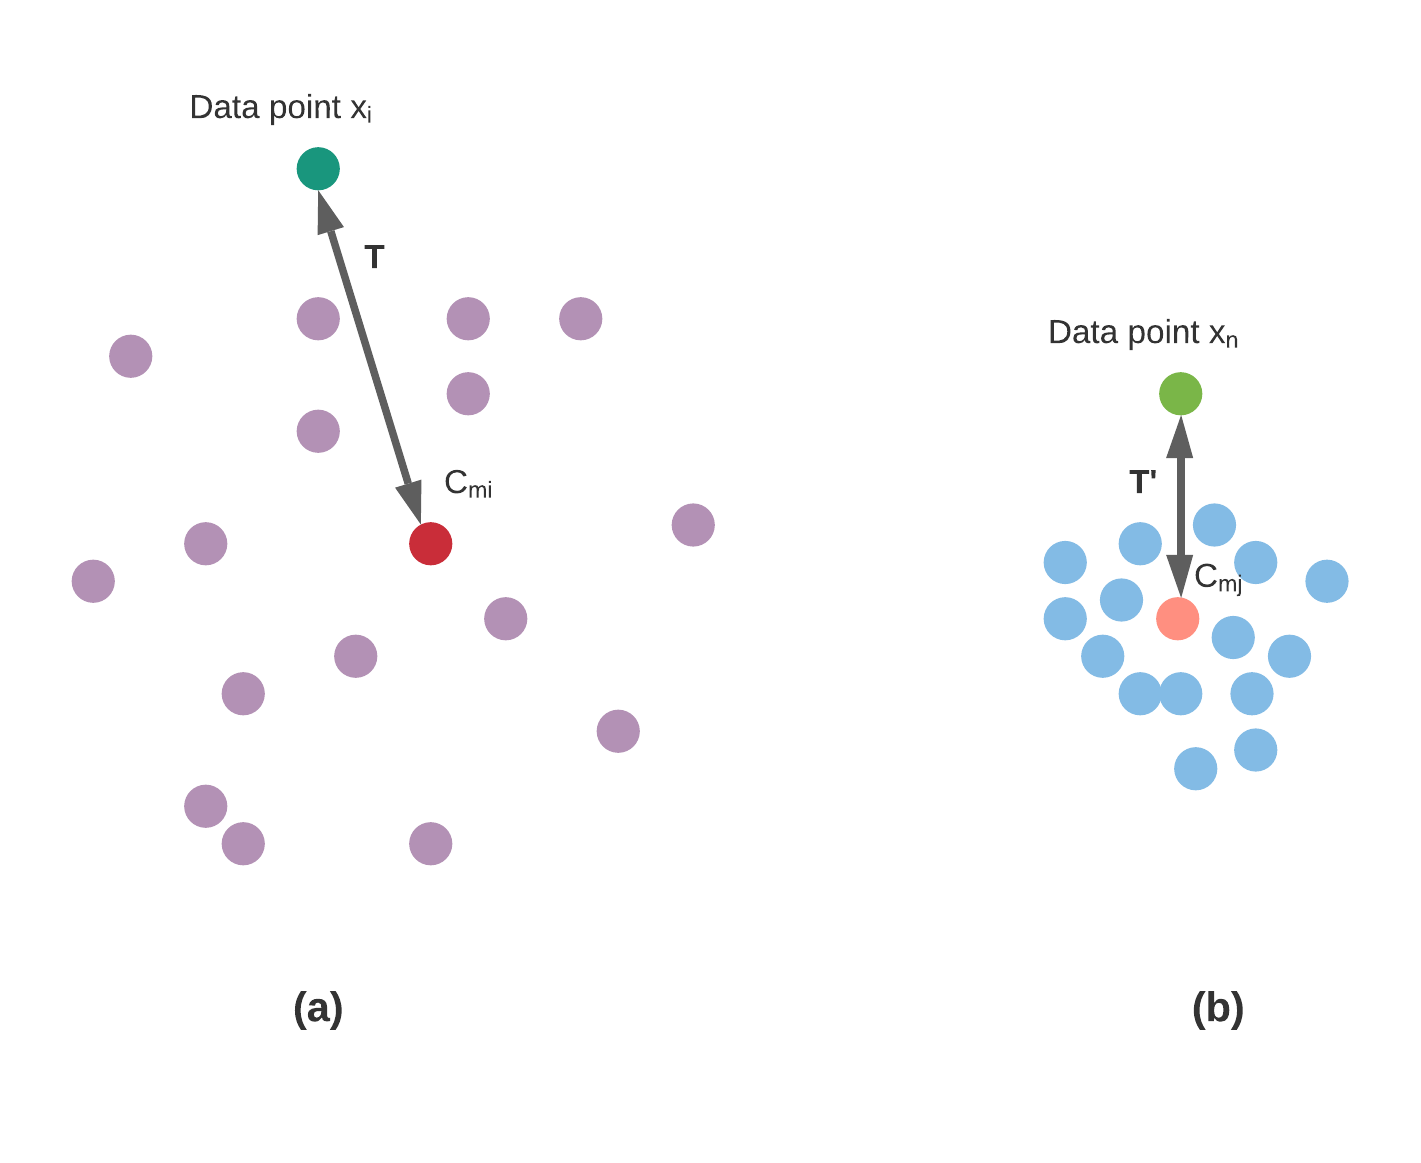
\includegraphics[width = 11 cm]{image/threshold.png}
    \caption{The impact of spread (a) and dense (b) cluster structures on comparing the closeness of new data points to existing micro-cluster centroids $C_m$ } 
    \label{thr}
    \end{figure}

The outputs of this step are the set of micro-clusters from the previous window, but now with new data points associated with some of the centroids, and an updated timestamp corresponding to the chosen centroids. Additionally, $n$ number of data points whose euclidean distance from the centroids was greater than $\epsilon_{W_j}$ are temporarily kept in the time-window repository.

%\todo[inline]{write down what the the outcomes are of this step}
    
    
    
\item[]\textbf{ActivateAP and Update  $\epsilon_{W_j}$}


    %The memory can fill up quickly if the data distribution changes. It is difficult to model a data stream with changing data distributions. This problem is referred to as concept-drift, that can lead to less accurate models as time passes. To handle concept-drift, the model needs to be consistently updated by moving the prime centroids of the clusters as the data evolves with time. Every once in a while when the number of data points in the repository exceeds a pre- defined value or at the end of the expiration time interval, the data points in the repository are clustered using AP. The expiration time ($T_{ex}$) is defined as time duration within which a data point stays relevant. It is set to a duration of $N_w$ times the window size ($T_{ex} = N_w*length(W_i)$) and is a user-defined parameter. After the AP is applied to the data points from the repository, new cluster centroids referred to as potential centroids ($[PC]$) are obtained. The potential centroids are compared with the prime centroids ($[C_{m0}]$). If the distance of any potential centroids from the prime centroids, $d(PC_i,Cm0_i)$ is less than the repository threshold $\gamma$ they will be grouped with the prime centroids for one final round of AP. This additional step of clustering centroids both prime and potential leads to the creation of new prime clusters as shown in Figure. \ref{frame}. Otherwise, if the distance is greater than the threshold, they will be added as a new prime centroid to the pool of prime centroids. After the AP is applied to the data points from the memory, new micro-clusters referred to as ($[PC]$) are obtained. This step of clustering leads to the creation of new micro-clusters. The outcome from this phase are a number of updated micro clusters ($C_{m0}$) that will be used to find macro clusters in the next phase.
    
   % new clusters are computed using the dta points which were stored in window 1
    
    
   % The data distribution changes over time. To have an accurate model as time passes, the model needs to be consistently updated as the data evolves with time.
    
    %All the data points in the current landmark window of length $L$ have been compared with the micro-clusters centroids, and if this distance is greater than the threshold, then the data point place in a temporary cache. 
    
    All the data points that have been temporarily accumulated during the execution of the previous step are used to compute new micro-clusters $C_m'$ using the AP algorithm once again. These new clusters will be added to the existing clusters $C_m$ that belong to their respective landmark time windows. As a result, the updated $C_m$ = $C_m'$ + $C_m$ is achieved. The new micro-clusters will have their respective timestamps associated with them.
    

    %Finally, these new clusters are added to the previous micro-clusters $Cm$, and the model is being updated ($Cm = Cm' + Cm$). 
    The next task is to compute the new $\epsilon_{W_j}$ by taking into account the centroids of the new micro-clusters found within a particular landmark window. This is accomplished by computing the mean of the intra-cluster distances using the new micro-clusters. The update $\epsilon_{W_j}$ is computed by applying the mean between the new and the current $\epsilon_{W_j}$. The updated $\epsilon_{W_j}$ is then used when the forthcoming data points from a new landmark time window arrive.
    
    
  
    
    %These points potentially represent new clusters. By applying the AP algorithm once again, new micro-clusters $Cm'$ are generated. Then, these new clusters $Cm'$ are added to the micro-clusters $Cm$ obtained before, and the model is updated ($Cm = Cm' + Cm$). The tasks performed during these steps are listed in Algorithm \ref{alg1} for better understanding.
    
  %\todo[inline]{how to get rid of old centroids... as soon as the centroids are not longer significant to compute the E , they are disregarded using the  factor. HOw do you do that??? } 

   In order to avoid the number of centroids to spread beyond control, old centroids that are no longer deemed relevant are removed. To do this, an expiration time parameter $e_x$ is introduced. This value is applied to forget centroids that haven't been selected in the recent windows as quantified by $e_x$. The $e_x$ number can be chosen to include all the time windows from the start or just the last few windows, depending on the user requirements. All the clusters whose associated timestamps are older than $e_x$ window lengths ($e_x \times L$) from the current time are considered obsolete and hence discarded. 
   %This value is obtained by subtracting the current time from the $ex$ number of time period. If any centroid in the previous time window seen in the current window, the timestamp associated to this centroid should be updated.
   
    % Increasing number of cluster usually lead to increasing time in processing the data, thus clustering process need to be broken down to prevent long process, this done by applying fading value to the process of clustering. 

% \begin{figure*}
% \centering
% \includegraphics[width = 15cm,height = 12cm]{image/tophase.png}
% \caption{The proposed DSAP flowchart }
% \label{frame}
% \end{figure*}



%After some time, the number of exemplars grows and maybe they become out of the control. To avoid this, we can remove the exemplar which has not been considered for a while. To implement this method, a specific time window $\triangle$ would be considered.
% \begin{equation}
%   \triangle_tj = t - t_j
%   \end{equation}

%After the new set of exemplars have been chosen, the list of outliers reset and new data points comes in to the model.


%%%%%%%%%%%%%%%%%%%%%%%%%%%%%%%%%%%%%%%%%%%%%%%%%%%%%%%%%%%%%%%%%%%%%%%%%%%%%%%%%%%%%%%%%%%%%%%%%
\end{itemize}


%need a table for notations and definitions! variables in the code
% which is illustrated in Figure \ref{frame} by the green box,
\subsection{Offline Macro-Cluster Phase}

The offline macro-cluster phase in DSAP, starts after $N$ time windows have passed. In this phase, all the micro-clusters $C_m$ generated during the online micro-cluster phase are re-clustered using the AP algorithm to generate $k$ number of macro-clusters $C_M = (C_{M_1}, C_{M_2}, ..., C_{M_k})$. This process is usually not considered time-critical and the number of macro-clusters are expected to be less than the number of micro-clusters. The hyperparameters related to the AP algorithm such as the the maximum number of iterations, and the convergence iteration are default values. The preference parameter is set to the median of the similarity matrix of all the micro-clusters obtained from the online phase, and the damping factor is fixed for all windows.


%\todo[inline]{Have you used the same hyperparameters??? Or they are changed??? e.g. number of interactions was the same for micro and macro clustering???} %Nasrin: No I don't change them. Just preference has been changed , which is the median of similarity matrix and I did not give it a number.

%The DSAP offline macro-clustering phase is composed of three steps. In the first step, the user requests for macro clusters from the online phase. Next, the list of micro clusters are retrieved from the online phase. The last step is to generate a set of macro clusters using the affinity-propagation clustering algorithm. AP gives macro clusters $[C_M]$ that summarizes all the micro clusters during the chosen interval. 




%The offline macro-clustering phase in DSAP,  which is illustrated in Figure \ref{frame} by green color, can be invoked by the user or pre-defined at regular intervals based on the data stream under consideration. In this phase, all the micro clusters $[C_{m0}]$ generated during the online phase are  re-clustered using another instance of the affinity propagation algorithm. The DSAP offline macro-clustering phase is composed of three steps. In the first step, the user requests for macro clusters from the online phase. Next, the list of micro clusters are retrieved from the online phase. The last step is to generate a set of macro clusters using the affinity-propagation clustering algorithm. AP gives macro clusters $[C_M]$ that summarizes all the micro clusters during the chosen interval. The pseudo-code presented in Algorithm \ref{alg1} succinctly summarizes the entire DSAP algorithm. 

%external: Rand index and Meila’s VI.
%One drawback of using internal criteria in cluster evaluation is the high scores on an internal measure do not truly result in data clustering. Additionally, this evaluation is biased towards algorithms that use the same cluster model. For example model used in k-Means clustering is naturally optimizes object distances, and a distance-based internal criterion will likely misjudge the resulting clustering.




\section{Intrinsic Clustering Validation Phase} \label{intrinval}

Intrinsic clustering validation uses the internal information of the clustering process to evaluate the goodness of a clustering structure when the ground truth labels are unknown. The well-known metrics silhouette index (S),  Caliński-Harabasz index (CH), and Davies-Bouldin index (DBI) were selected to validate the goodness of macro clusters found by the DSAP algorithm. Table \ref{comp} provides an overview of these metrics. They are further described in detail in the following sections.

%\todo[inline]{have you computed the metrics for micro and macro clusters??? or just macro clusters??} %Nasrin: Just Macro clusters

% \begin{table}[htbp]\scriptsize
% % \centering
% \caption{Intrinsic clustering metrics used for validation of clustering results.}
% \label{comp}   
% \begin{tabularx}{\linewidth}{|p{2cm}|p{5cm}|p{3cm}|p{3.4cm}|}
% \hline
%  \multicolumn{1}{|c|}{\textit{\textbf{Metric}}} &
%  \multicolumn{1}{|c|}{\textit{\textbf{Description}}} &
%  \multicolumn{1}{|c|}{\textit{\textbf{Advantages}}}   &   
% \multicolumn{1}{|c|}{\textit{\textbf{Disadvantages}}} 
% \tabularnewline \hline
% \vfill 
%  \raggedright Silhouette Index &  
% \vfill
%  It measures how similar a data point is to its own cluster compared to other clusters.
%  &
 
%  \begin{enumerate}[*,nosep,leftmargin=0.2cm]
%  \item Value bounded between [-1,1]  
%  \item High scores when clusters are well separated
% \end{enumerate}
% \tabitem
% &       
% \begin{itemize}[*,nosep,leftmargin=0.2cm]
%     \setlength\itemsep{0em}
%      \item High computational complexity
%      \item Higher value for convex clusters unlike density based clusters
% \end{itemize} 
% \tabularnewline \hline
% \vfill 
%  Caliński-Harabasz Index     &     
% \vfill
% It is the ratio between the intra-cluster dispersion and the inter-cluster dispersion.
% & 
% \begin{itemize}[*,nosep,leftmargin=0.2cm]
%     \item Fast to compute
%     \item Easy to interpret %as it gives higher value when clusters are dense
% \end{itemize}
%  &       

% \begin{itemize}[*,nosep,leftmargin=0.2cm]
%     \item Higher value for convex clusters% compared with density based clusters
% \end{itemize}
% \tabularnewline \hline
% \vfill 
% Davies-Bouldin Index        &       
% \vfill
% It is the average similarity measure of each cluster with its most similar cluster.%, where similarity is the ratio of within-cluster distances to between-cluster distances
% & 
% \begin{itemize}[*,nosep,leftmargin=0.2cm]
%     \item Simple to implement
%     \item Value is able to compute when features inheritent to the dataset
%     %\item Quantity computation ?????
% \end{itemize}
%          &      
         
% \begin{itemize}[*,nosep,leftmargin=0.2cm]
%     \item Higher values for convex clusters
%     \item Limited to Euclidean distance only
% \end{itemize}

% \tabularnewline\hline

% \end{tabularx}
% \end{table}
%%%%%%%%%%%%%%%%%%%%%%%%%%%%%%%%%%%%
\begin{table}[htbp]
\small
\caption{Intrinsic clustering metrics used for validation of clustering results.}
\label{comp}
\begin{tabular}{llll}
\hline
\multicolumn{1}{c}{\textbf{Metrics}}                                  & \multicolumn{1}{c}{\textbf{Description}}                                                                                                 & \multicolumn{1}{c}{\textbf{Advantages}}                                                                                                          & \multicolumn{1}{c}{\textbf{Disadvantages}}                                                                                                                  \\ \hline\midrule
\begin{tabular}[c]{@{}l@{}}Silhouette\\  Index\end{tabular}           & \begin{tabular}[c]{@{}l@{}}It measures how similar\\ a data point is to its own\\ cluster compared to \\ other clusters.\end{tabular} & \begin{tabular}[c]{@{}l@{}}* Value bounded \\  between {[}-1,1{]}\\ * High scores when \\ clusters are well\\  separated\end{tabular}             & \begin{tabular}[c]{@{}l@{}}* High computational\\    complexity\\ * Higher value for \\    convex clusters  unlike\\    density-based clusters\end{tabular} \\ \hline
\begin{tabular}[c]{@{}l@{}}Caliński-\\ Harabasz \\ Index\end{tabular} & \begin{tabular}[c]{@{}l@{}}It is the ratio between\\ the intra-cluster \\ dispersion and the\\ inter-cluster dispersion.\end{tabular}    & \begin{tabular}[c]{@{}l@{}}* Fast to compute\\ * Easy to interpret\end{tabular}                                                                  & \begin{tabular}[c]{@{}l@{}}* Higher value for\\    convex clusters\end{tabular}                                                                             \\ \hline
\begin{tabular}[c]{@{}l@{}}Davies-\\ Bouldin\\  Index\end{tabular}    & \begin{tabular}[c]{@{}l@{}}It is the average\\  similarity  measure\\ of each cluster with \\ its most similar cluster.\end{tabular}     & \begin{tabular}[c]{@{}l@{}}*Simple to implement\\ *Value is able to com-\\    pute when features\\    inherent to the \\    dataset\end{tabular} & \begin{tabular}[c]{@{}l@{}}* Higher values for \\    convex clusters\\ * Limited to Euclidean\\    distance only\end{tabular}                               \\ \hline\midrule
\end{tabular}
\end{table}








\subsection{Silhouette Index}

 The silhouette index was introduced by \cite{rousseeuw1987silhouettes} on the premise of the  silhouette  width  of  a  data  point to measure how similar a data point is to its own cluster compared to other clusters. The silhouette index $S_i$ for a data point $i\in x$ in cluster $C_k\in C$ is calculated using Equation \ref{sil}.
 
 %\todo[inline]{missing reference rousseeuw1987silhouette}
 
 \begin{align}
    a_i = \frac{1}{C_k} \sum_{j \in C_k,i\neq j } d(i,j) \\
    b_i = \min_{C_m \in C, C_m\neq C_k} \frac{1}{\abs{C_m}} \sum_{j \in C_m,i\neq j} d(i,j) \\
    s_i =  \frac{b_i - a_i}{\max(a_i,b_i)}  \label{sil}
\end{align}

The first parameter $a$ is the average distance between the sample and all the others in the same class, and the second parameter $b$ is the mean distance between the sample and all the other points in the next closest cluster. Negative $S_i$ scores for a point $i$ means that the data point is in the incorrect cluster. Positive scores show a robust and dense clustering. Moreover, values around zero indicate overlapping clusters. If the $S_i$ has a higher value, it means a greater ratio between $b_i$ as compared with $a_i$, causing the data point $i$ to be more similar to the other data points in the same cluster.  

The primary advantage of the silhouette index is its straightforward interpretation. The score is bounded between -1 for incorrect clustering and +1 for highly dense clustering. Scores around zero indicate overlapping clusters. The score is higher when clusters are dense and well separated, which relates to a standard concept of a cluster. However, it has a high computational complexity of $O(n^2)$. Additionally, it is well known that the coefficient values tend to be higher for convex clusters as compared to other uniquely shaped density based clusters.


%\begin{figure}
    %\centering
   % 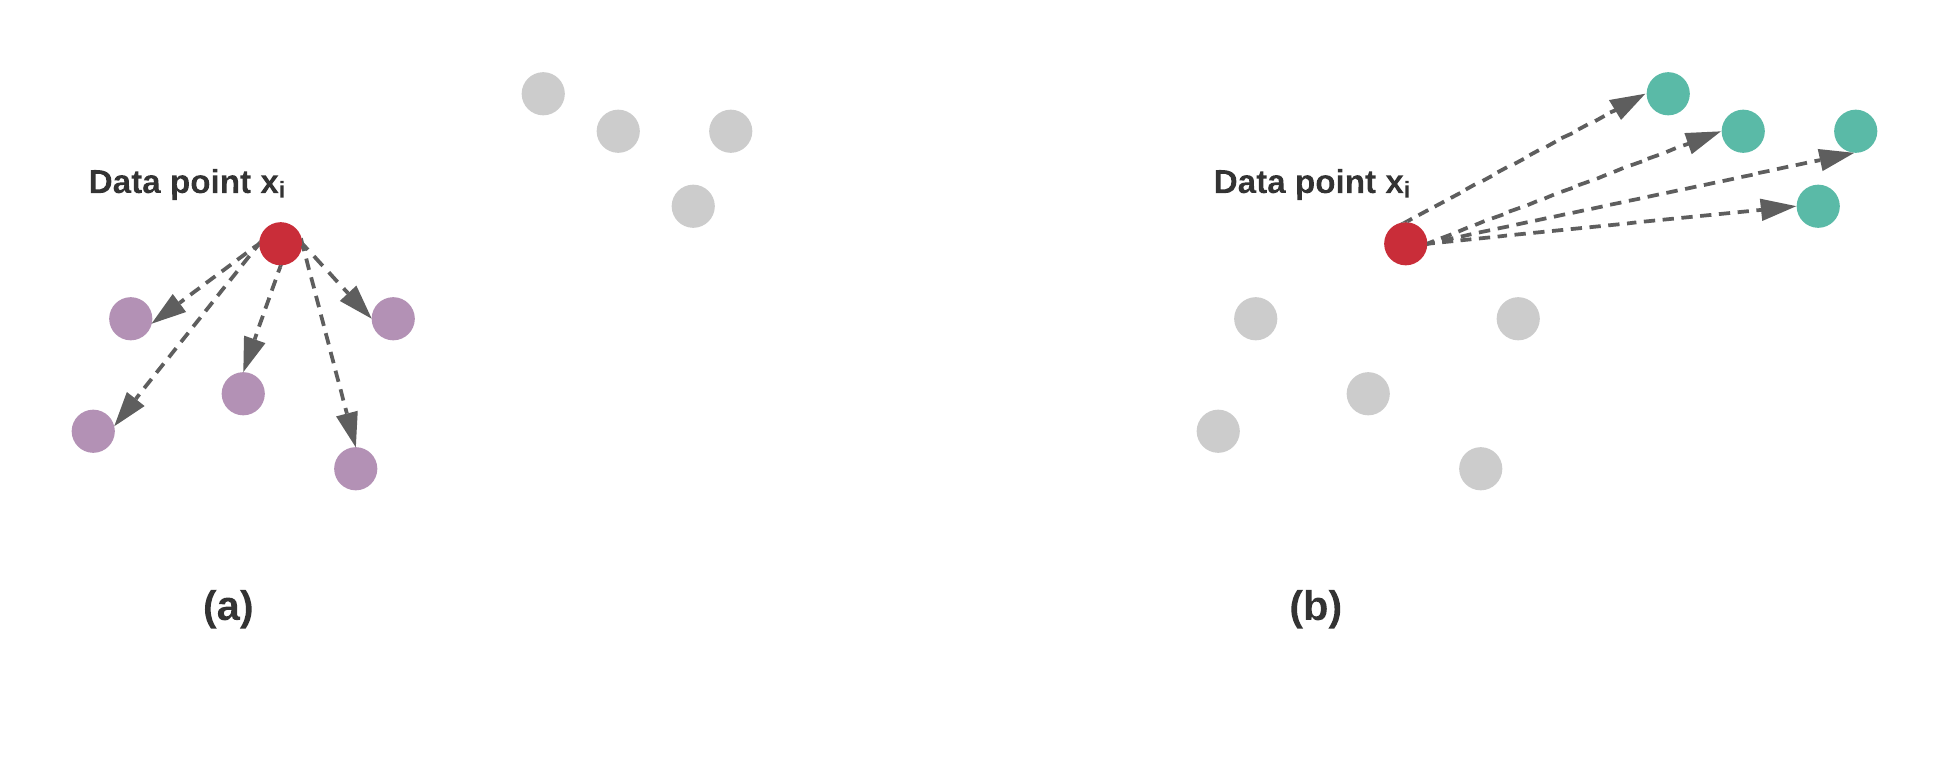
\includegraphics[width = 11 cm]{image/silo.png}
   % \caption{Silhouette Coefficient for a data point $x_i$, calculates for all data points in its own cluster(a), and for all other data points in other clusters (b).}
   % \label{silo}
%\end{figure}
    

\subsection{Caliński-Harabasz Index}
It is also known as the variance ratio criterion, which is used to score dense and well-separated clusters. A recent comparative study of available clustering indices demonstrated this index as one of the best cluster validity indices \cite{arbelaitz2013extensive}. 

%\todo[inline]{not sure if you have cited this paper}%Fixed it

Well defined clusters yield high values of this index. Therefore, the maximum value of the index is used to select the best partition. For \begin{math} n \end{math} data points, \begin{math} k \end{math} clusters  where \begin{math} B \end{math} and \begin{math} W \end{math} are the between within cluster scatter matrices, the index is computed as \cite{calinski1974dendrite}:

%\todo[inline]{not sure why the reference calinski1974dendrite is not being compiled}

\begin{equation}
  CH =  \frac{traceB / (k - 1)} {traceW/ (n -k)}
\end{equation}   


%For a  data point $i$ of size $I$ which has been clustered into $k$ clusters, the Calinski-Harabasz score $s$ is defined as the ratio of the mean dispersion between clusters and the within cluster dispersion:

%\begin{equation}
    %s = \frac{\mathrm{tr}(B_k)}{\mathrm{tr}(W_k)} \times \frac{n_i - k}{k - 1}
%\end{equation}
where
\begin{equation}
    B_k = \sum_{q=1}^k n_q (c_q - c_i) (c_q - c_i)^T
\end{equation}

\begin{equation}
    W_k = \sum_{q=1}^k \sum_{x \in C_q} (x - c_q) (x - c_q)^T
\end{equation}

with $C_q$ the set of points in cluster $q$, $c_q$ the center of cluster $q$, $c_D$ the center of $D$, and $n_q$ the number of points in cluster $q$.

%The $tr(B_k)$ is a dispersion matrix effect between groups of data and $tr(W_k)$ is the effect of the within-cluster dispersion matrix defined by $B-k$


The CH is computationally efficient to calculate, but just like the silhouette index, the CH index is biased towards convex clusters assigning them higher values than the density based clusters such as those obtained through DBSCAN.

\subsection{Davies-Bouldin Index}

Davies-Bouldin Index (DBI) was introduced in 1979 by \cite{4766909}, and it computes the average similarity between each cluster $C_i$ for $i = 1,2,...,k$ and its most similar one $C_j$.  For this index, similarity is defined as a measure $R_{ij}$ that optimizes:

\begin{itemize}
    \item $s_i$: the average distance between each data point in the cluster and the centroid of that cluster.
    \item $d_{ij}$: the distance between cluster centroids $i$ and $j$.
\end{itemize}

A simple choice to construct $R_{ij}$ is that of non-negative and symmetric as follows:

\begin{equation}
    R_{ij} = \frac{s_i + s_j}{d_{ij}}
\end{equation}

Then the Davies-Bouldin index is defined as:

\begin{equation}
    DB = \frac{1}{k} \sum_{i=1}^k \max_{i \neq j} R_{ij}
\end{equation}

 With this index, a minimum value denotes the best partitioning of the data. The average similarity calculation is much simpler than the computations required for calculating the silhouette index. Like the previous two metrics, DBI too suffers from a preference towards convex clusters as compared to density based clusters owing to the usage of centroid distance that limits the distance metric to Euclidean space.





% \subsection{Comparison of Intrinsic Clustering Metrics}
% The three metrics discussed above have some advantages and drawbacks which they are listed below.
% \begin{itemize}
%     \item The advantage of using the Silhouette Coefficient is this score has a range between -1 and 1. The high score shows that the data point is well matched to its own cluster and clusters are dense, and the low value shows a poor match to the neighboring clusters. On the other hand, the Silhouette Coefficient is a data-related metric, and it means it is higher for convex clusters than other types of clusters such as density based clusters like DBSCAN. Also, the time complexity for this score is $O(n^2)$ which is high.
    
%     \item The advantage of applying the Calinski-Harabasz Index is it is fast to compute the number, and it shows the density of the clusters with a higher value, which is related to the concept of a cluster. However, the drawback is this score is mostly higher when the clusters are convex.
    
    
%     \item The advantage of having Davies-Bouldin Index is that computing this metric is simpler than computing the Silhouette Coefficient. Also, this value is able to compute when features inheritent to the dataset. 
%     The drawback of the index is as the other metrics mentioned before, is being higher for convex clusters such as density based clusters like DBSCAN, and 
%     (change)the usage of centroid distance limits the distance metric to Euclidean space.
% \end{itemize}



% Please include the text below:
% Comparison between these metrics:

% Silhouette Coefficient
% Advantages
%     The score is bounded between -1 for incorrect clustering and +1 for highly dense clustering. Scores around zero indicate overlapping clusters.

%     The score is higher when clusters are dense and well separated, which relates to a standard concept of a cluster.

% Drawbacks

%     The Silhouette Coefficient is generally higher for convex clusters than other concepts of clusters, such as density based clusters like those obtained through DBSCAN.

%     High computational complexity: O(n²)
    
    
% Calinski-Harabasz Index
% Advantages
%     The score is higher when clusters are dense and well separated, which relates to a standard concept of a cluster.

%     The score is fast to compute.

% Drawbacks

%     The Calinski-Harabasz index is generally higher for convex clusters than other concepts of clusters, such as density based clusters like those obtained through DBSCAN.

% Davies-Bouldin Index
% Advantages
%     The computation of Davies-Bouldin is simpler than that of Silhouette scores.

%     The index is computed only quantities and features inherent to the dataset.

% Drawbacks
%     The usage of centroid distance limits the distance metric to Euclidean space.

%     The Davies-Boulding index is generally higher for convex clusters than other concepts of clusters, such as density based clusters like those obtained from DBSCAN.


%\item\textbf{Clustering-based Outlier Detection:}
%The purpose of outlier detection is to separate a core of general observations from the polluting ones or outliers. They can be noise or an interesting data points and in both cases outlier detection is important. Also the number of outliers have a relationship with the model efficiency. These outliers can effect the quality of the model and the centroids of each clusters. Either these data points do not belong to any other clusters or to the clusters which are far from other clusters. To find how the DSAP is efficient in detecting outliers, we inject specific number of data points to our algorithm to see how it can affect our result. 

% To find out which algorithm is support robust in terms of  outliers, Support Vector Data Description (SVDD) algorithm is employed by generating hyper sphere for the data.  
%Based on the Equation \ref{out}, if $O_i$ is the $i^{th}$ cluster, $|O_i|$ be cardinality of $O_i$ and $j$ is the cluster count, then $O_m$ is the outlier if: 
% \begin{equation}
%     \abs{O_m} << \frac{1}{j} \sum_{i=1}^{j} \abs{O_i}\label{out}
% \end{equation}

\section{Clustering Performance Evaluation Phase}

Data stream clustering brings about a few unique challenges as compared to traditional data clustering. The data streams are a continuous flow of data points that arrive at rapid rate. Random access to these data points is not possible and the volatility of the data streams sometimes limits to having a single look at the data points upon their arrival. 

%As a result there is a need for fast processing of each data point that arrives from the stream and maintain summaries of the data instead of the raw data to save memory. 

To evaluate the efficiency of the DSAP, two metrics are proposed: computational time and the memory consumed to run the DSAP algorithm. These metrics used in this phase are described in the next sections.

\subsection{Time Complexity}

The efficiency of any algorithm can be estimated using the time complexity, which can be defined as the time taken to run the number of elementary operations performed by the algorithm given an input array of length N. In other words, it is the amount of time taken by an algorithm to run, as a function of the length of the input.  

The most frequently performed action within the algorithm whose execution time does not change with the size of the input array is called the elementary operation. The most common metric used for estimating time complexity is the Big O notation. The big O notation is typically used to illustrate the worst-case growth of an algorithm (or how the run time/space requirements of an algorithm increase with input size), which excludes coefficients and lower order terms.

In real-world applications, in addition to the time complexity, several other factors can affect the execution speed. Many concurrent tasks like receiving network traffic, checking the hard disk, and writing log files, are performed by a typical computer while it performs the clustering tasks. The data-dependent rate of convergence of the algorithms also affects the total execution time. Therefore, it is recommended to run a task multiple times to get average values after discarding the initial few results as they could be affected by the time-window repositoryd results. %Plot the spread over multiple runs to choose a cutoff.
%Rough estimates of the start and end times of the algorithms can be noted by native functions available under each programming language.


\subsection{Space Complexity} 
Similar to the time complexity, the memory consumption quantifies the amount of memory taken by an algorithm to run as a function of the length of the input. That means how much memory, in the worst case, is needed at any point by the algorithm. The same big-O notation is used to describe the space complexity as well. This parameter represents the algorithm’s scalability and performance. In simple terms, it gives the worst-case scenario of an algorithm’s growth rate.

To calculate space complexity, we need to know the value of memory used by different types of datatype variables, which generally vary for different operating systems. Hence it is not straightforward to provide generic formulations for the spatial complexity of any algorithm.

To compare different algorithms, we have to make sure that they have been suitably implemented since poor memory management can lead to a superior algorithm under-performing as compared with the superior implementation of a less efficient algorithm. Analogous to the time metric, it is necessary to test the algorithms on data sets of multiple sizes for an accurate assessment of the memory usage. 


% \section{Comparison  Between  DSAP  and  Streaming  K-means Phase}

% move the paragraphs here to other sections

% - difficult to find available source code for previusouly proposed stream AP, etc...


% The general approach of the various stream clustering algorithms that allow for the investigation of the cluster structure at different time intervals are fairly similar. They typically have two stages, online where the algorithm maintain a summary of the data as micro-clusters and next in the offline phase the summary micro-clusters are clustered to provide real insights to the data. The efficiency of these algorithms are greatly affected by the choice of the clustering algorithm used. We have introduced the DSAP algorithm for data stream clustering which is implemented based on the AP algorithm. This model is compared with the established streaming K-means algorithm introduced earlier in Chapter 2. It is known that the AP algorithm usually generates results that show that the k-means algorithm is faster than AP. However, streaming AP based algorithms has been shown to provide similar quality clusters as k-means based ones but, the results tend to be more robust.

% K-means algorithm is scalable for large datasets with different shapes and sizes and is easy to implement. The K-means algorithm is known to easily adopt to new centroids and is one of the fastest algorithms out there owing to a linear time complexity. Also, K-means guarantees convergence by trying to minimize the total sum of the square error as an objective function over the number of iterations. On the other hand, the K-means algorithm has some known drawbacks. Finding the $k$ optimum number of clusters is not a precise task that can be accurately automated. The algorithm results are a function of the initial clusters chosen and necessitate multiple runs of the algorithm with the different values to pick the most suitable clusters. During data stream clustering this process can be time consuming and make the model less accurate. The algorithm is known to have difficulties in finding the right clusters for data with varying size and density. In addition, K-means clusters centroids are affected by outliers since the mean as a statistic is sensitive to outliers. %it means outliers can drag the centroids or they may have their own centroids. 
% Lastly, even though K-means can be easily scaled to large datasets but it has difficulties to cluster high-dimension data. 


% In comparison with the K-means algorithm that needs to determine the optimal number of clusters prior by applying some methods like elbow method, the AP algorithm calculates the number of clusters internally. However, AP needs additional parameters like the damping factor and preference to be set since the model convergence is dependent on the damping parameter while the preference controls the probability of finding centroids. Due to the additional complexities in the calculation of AP it becomes prohibitively expensive to scale AP as compared to the K-means which scales linearly with the size of the dataset. The semi-supervised selection of the number of clusters in K-means limits the potential of producing large number of clusters that can sometimes be generated by the AP if it's parameters are not chosen carefully. Both these partitioning based algorithms can be evaluated based on metrics that quantify the density and spread of the clusters. 

% Affinity propagation has been shown to perform well in pattern recognition applications in the fields of computer vision and computational biology. The main advantage of AP is the robustness of its optimization. While K-means follows a greedy optimization method to find the optimum of the optimization problem, AP tackles a continues optimization problem, in which all data points are potential candidate at the beginning and clusters are gradually identified. AP does not suffer from the initialization can guarantee global optimization consistently.

\section{Summary}

Figure \ref{frame} summarizes the entire research methodology discussed in this chapter. The four phases of the DSAP approach are depicted with their main steps and respective tasks. 



%were discussed. Figure based on four phases is introduced along with the various quality and performance evaluation techniques. This algorithm consists of two phases, online micro-cluster and offline macro-cluster. These two phases are depicted with the grey and green boxes in the flow chart shown in Figure \ref{frame} that summarizes the entire research methodology discussed in this chapter. The online phase finds the updated micro-clusters from the stream by applying landmark window. The offline phase generates macro-clusters, a summary of all data points from the stream by re-clustering the micro-clusters. 

\begin{figure}[h]
\centering
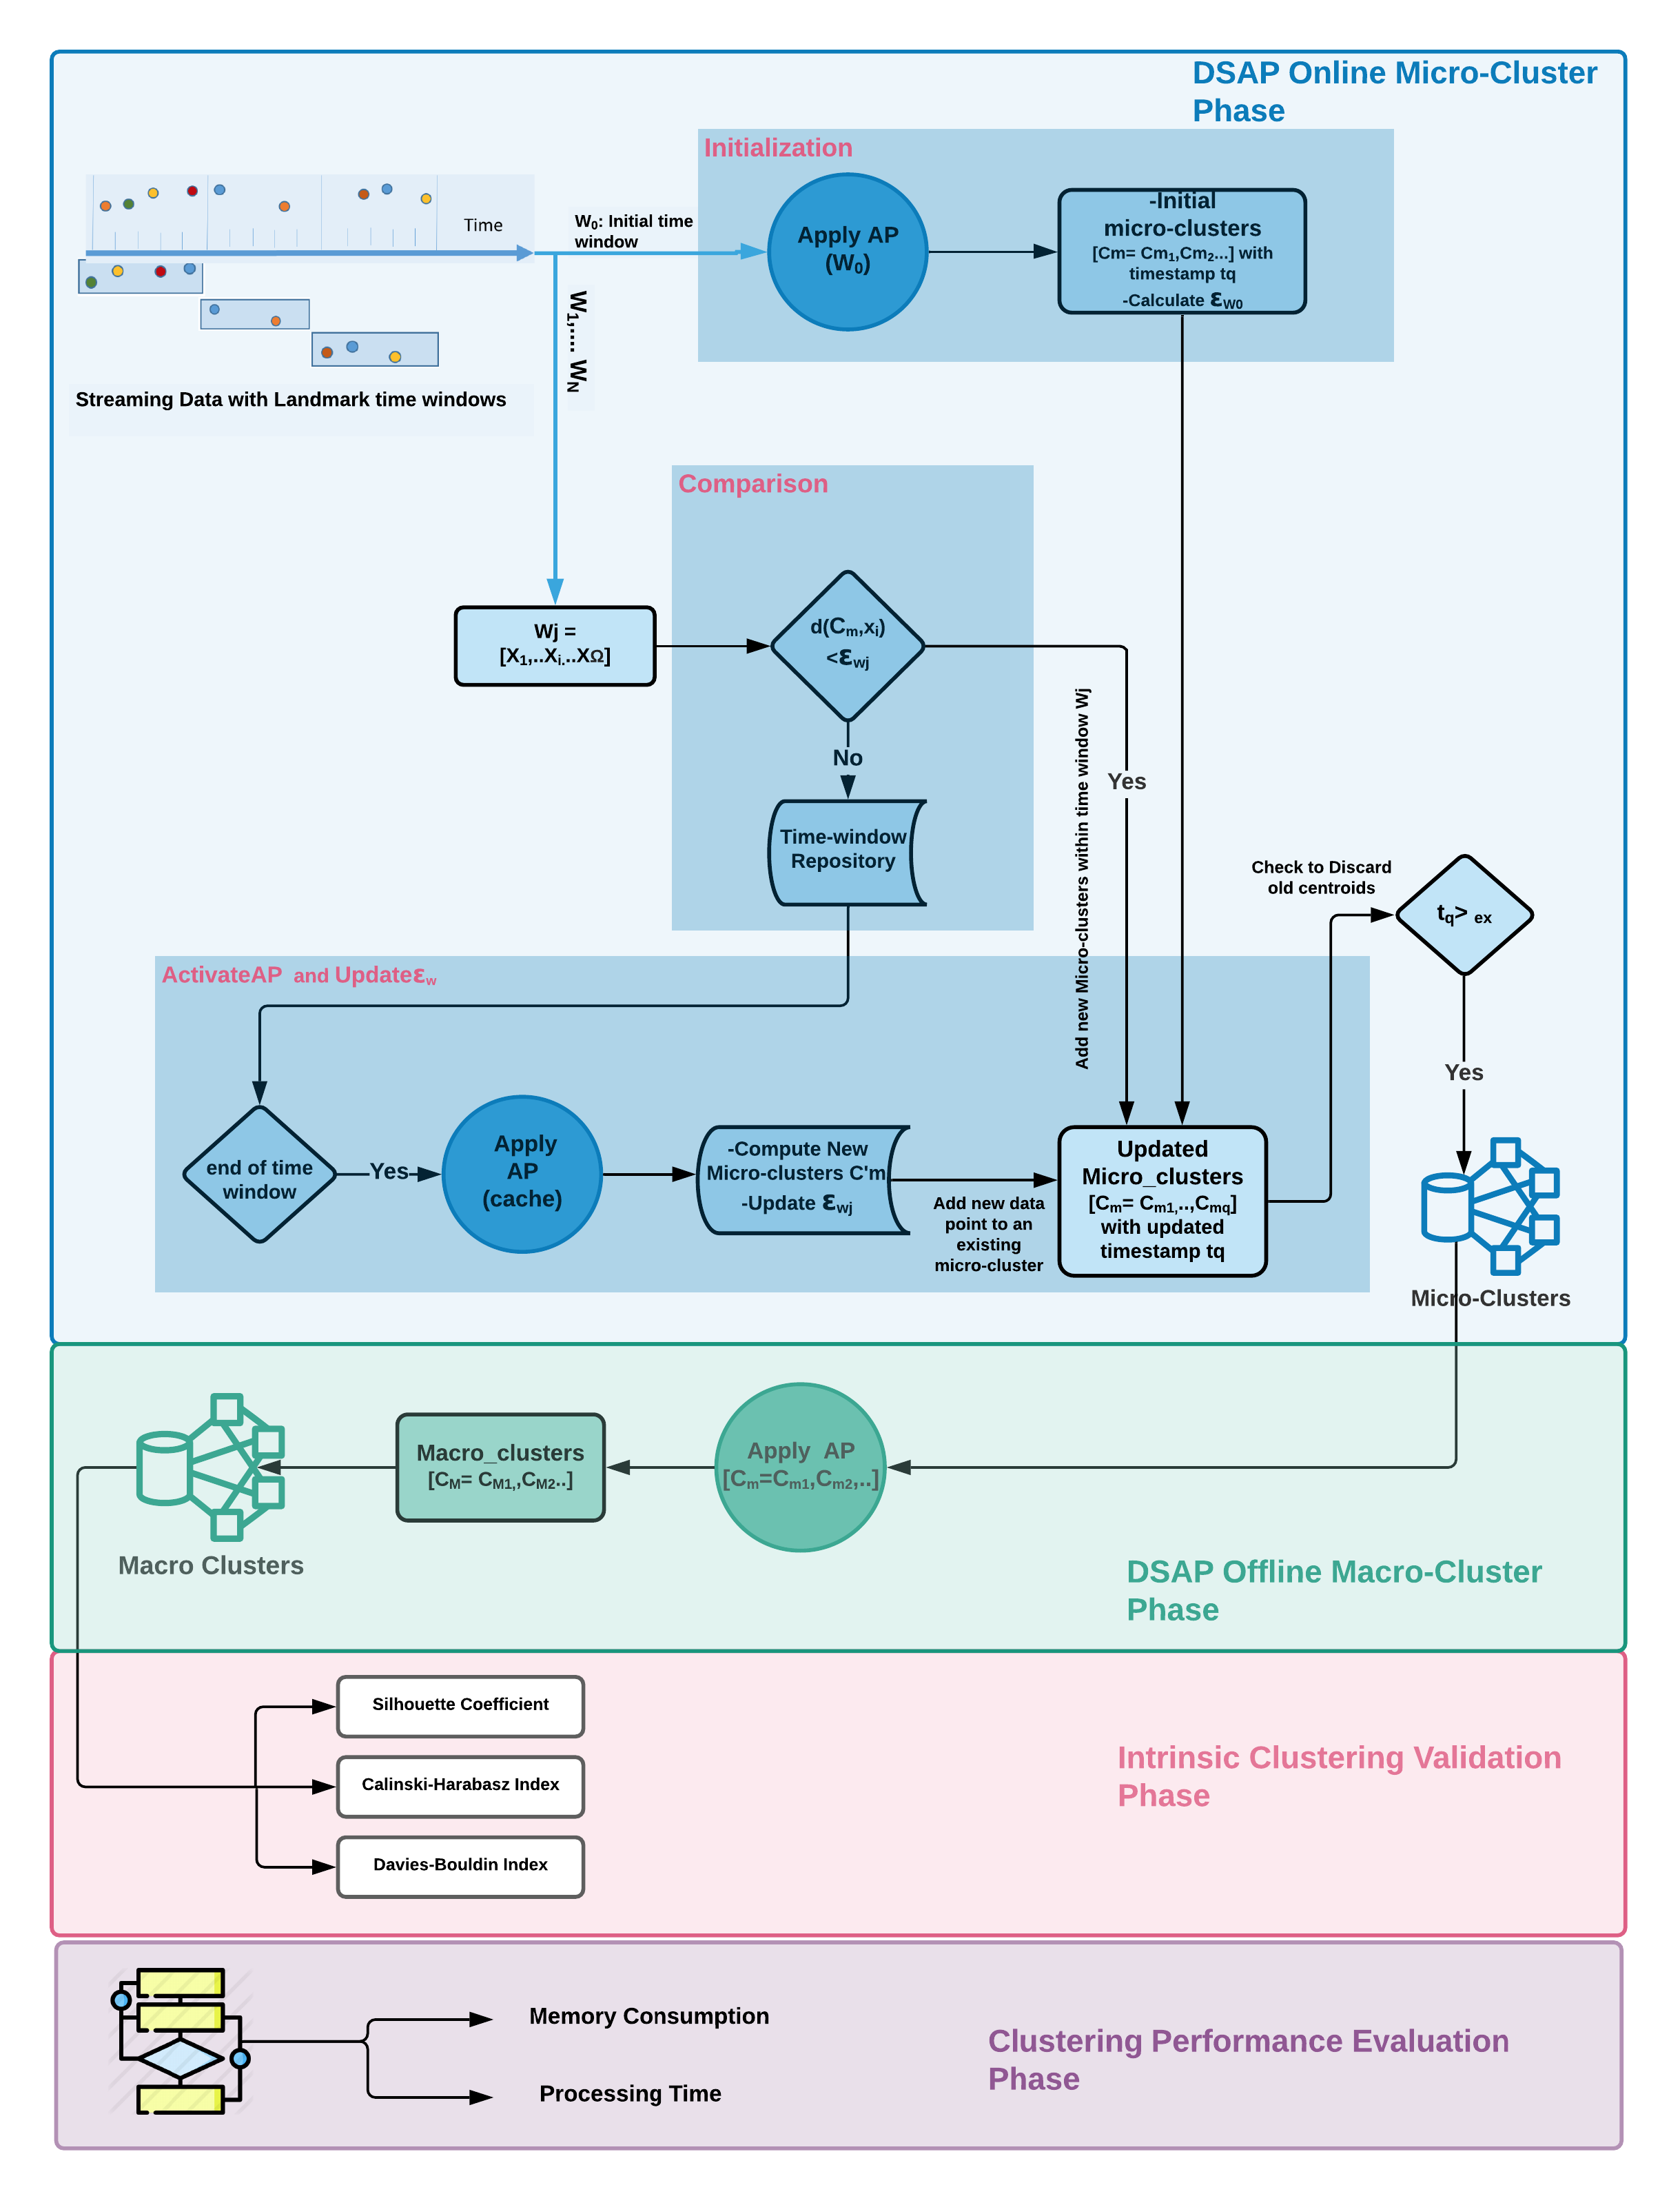
\includegraphics[width =1.05\textwidth]{image/Chapters/Chapter4/dsapflowchart1.png} 
\caption{Flowchart of the proposed DSAP approach}
\label{frame}
\end{figure}

The online micro-cluster and offline macro-cluster phases are are depicted within the grey box in blue and green colors respectively in the flow chart shown in Figure \ref{frame}. The online phase initializes the computation of micro-clusters and computes the updated micro-clusters from the new data points harvested using the landmark time window. The offline phase generates macro-clusters, a summary of all data points from the stream by re-clustering the micro-clusters. 

The silhouette index, Caliński-Harabasz index, and Davies-Bould in index are proposed to assess the goodness of  the clustering structures of the discovered micro and macro clusters since the ground truth labels were unknown. This phase is illustrated in Figure \ref{frame} with bright red color. The efficacy of any stream clustering algorithm is tied to its memory consumption and speed of execution. In order to evaluate this, in the Clustering Performance Evaluation phase shown in Figure \ref{frame} with purple color, the time and space complexity of the DSAP algorithm are estimated. 



















% Monica. EXPLAIN WHY THIS COMPARISON IS IMPORTANT
% 1. AP has usually produced results that have shown the k-means was faster than AP
% 2. However DSAP has shown to provide similar performance as k-means

% ---------------------- source https://developers.google.com/machine-learning/clustering/algorithm/advantages-disadvantages -------------------------------------
% -----------------------
% Advantages of k-means : Scales to large data sets. Guarantees convergence. Can warm-start the positions of centroids. Easily adapts to new examples. Generalizes to clusters of different shapes and sizes, such as elliptical clusters.

% Disadvantages of k-means
% Choosing  manually.

% Use the “Loss vs. Clusters” plot to find the optimal (k), as discussed in Interpret Results.

% Being dependent on initial values.

% For a low , you can mitigate this dependence by running k-means several times with different initial values and picking the best result. As  increases, you need advanced versions of k-means to pick better values of the initial centroids (called k-means seeding). For a full discussion of k- means seeding see, A Comparative Study of Efficient Initialization Methods for the K-Means Clustering Algorithm by M. Emre Celebi, Hassan A. Kingravi, Patricio A. Vela.

% Clustering data of varying sizes and density.

% k-means has trouble clustering data where clusters are of varying sizes and density. To cluster such data, you need to generalize k-means as described in the Advantages section.

% Clustering outliers.

% Centroids can be dragged by outliers, or outliers might get their own cluster instead of being ignored. Consider removing or clipping outliers before clustering.



% -----------------------
% DIFFERENCES BETWEEN K-MEANS AND AP

% Differences between K-means and affinity propagation:

% Parameters on initialization:
% KM: number of clusters.
% AP: damping damps the responsibility and availability messages, sample preference controls the number of exemplars.
% Scalability:
% KM: scalable with the number of samples.
% AP: not scalable with the number of samples.
% Usecase:
% KM: General-purpose, even cluster size, flat geometry, not too many clusters.
% AP: Many clusters, uneven cluster size, non-flat geometry.
% Metric used:
% Distances between points.
% Graph distance.
% Application:

% Affinity propagation was shown to perform well on the following tasks:computer vision.
% biology tasks.
% -----------------------------------------------

% ADVANTAGES OF AP: Affinity Propagation is much more
% tolerant to errors, it can remove the oscillation when it occurs
% where the occupance of oscillation will bring the algorithm to fail
% to converge. Adaptive Affinity propagation is more stable than
% the other since it can deal with error which the other can not.
% And Fuzzy Statistic Affinity Propagation can produce smaller
% number of cluster compared to the other since it produces its
% own preferences using fuzzy iterative methods.
% --------------------------------------------


% \end{document}


% the drawback of applying K-means clustering algorithm is that is need to calculate the number of clustre prior 

 % \begin{equation}
    % d^i_{min}   = min [{d(E^{i-1}_{m}, W^i), d(E^{i-1}_{m'}, W^i)}]
    % \end{equation}
    %To control the number of centroids to not exceed beyond the control, the old centroids have not visited for a long time, should be remove. To do this, the centroids will be deleted over the time. 
    % wite inja  tedad marakez ziad beshe
    
    %\item\textbf{re-establishing:}
    %add the decay value: This repository has the latest window and is identified by the decay factor.
%%---------------Chapter 5------------------------------
% \documentclass[../UNBThesis2.tex]{subfiles}
\setlength{\parindent}{2em}
% \usepackage{caption}
% \usepackage{subcaption}
% \usepackage{floatrow}
% \usepackage[label font=bf,labelformat=simple]{subfig}
% \floatsetup[figure]{style=plain,subcapbesideposition=botton}

%itemize without indent :\setlength{\itemindent}{-1.5em}
%single paragraph indent --> /noindent

%short term memory

\definecolor{dkgreen}{rgb}{0,0.6,0}
\definecolor{gray}{rgb}{0.5,0.5,0.5}
\definecolor{mauve}{rgb}{0.58,0,0.82}

\lstset{frame=tb,
  language=Python,
  aboveskip=3mm,
  belowskip=3mm,
  showstringspaces=false,
  columns=flexible,
  basicstyle={\small\ttfamily},
  numbers=none,
  numberstyle=\tiny\color{gray},
  keywordstyle=\color{blue},
  commentstyle=\color{dkgreen},
  stringstyle=\color{mauve},
  breaklines=true,
  breakatwhitespace=true,
  tabsize=3
}






% \begin{document}

\chapter{Implementation}

In this Chapter, the design and implementation of the DSAP algorithm are described. Next, two case studies are presented that are related to applying the proposed DSAP model to find mobility patterns in an indoor environment. 

%The two studies are: an e-counter based Indoor staircase usage experiment and a WiFi fingerprint-based Indoor Localization dataset. 


%The DSAP algorithm is a clustering approach consisting of phases as shown in Figure \ref{frame}. The online micro-cluster phase detects newly arriving data points and updates the clusters. The offline macro-cluster phase generates summary clusters periodically or at the end of the stream. The intrinsic clustering validation Phase ,and clustering performance evaluation phase assesses the clustering quality based on different criteria. The last phase, comparison between DSAP and streaming K-means shows the DSAP results compare to the streaming K-means results.






%\section{DSAP Clustering Algorithm}
%The Data Stream Affinity Propagation (DSAP) algorithm is an online and offline algorithm that generates micro and macro clusters based on a landmark time window model. This section describes the DSAP algorithm, which extends the AP algorithm for streaming data clustering applications. 

%Considering the challenges of clustering data streams to have updated clusters, this algorithm generates a model that describes the data streams and incrementally updates the model to generate recent clusters with any type of data. The DSAP algorithm consists of two phases: online phase and offline phase. these two phases receive and analyze data streams in real-time. However, the two datasets that are analyzed in this work were obtained from experiments performed over a fixed time period. For this reason, we had to convert the data into a simulated data streams, we discuss about this approach in the next section.

\section{Data Stream Simulation}
%Data elements in the stream arrive online, there is no control over the order in which elements arrive, either within a single stream. Streams are potentially unlimited in size

% #####################################
%  Using affinity propagation for streaming clustering faces two difficulties. First, AP has been implemented for batch processing but it should handle data clustering and large datasets in the online mode. The most important point to consider is AP suffers from quadratic computational complexity.
% Extensive data that are continuously coming are required to store. Analyzing big datasets and extracting patterns is not possible with affinity propagation due to the time complexity issue.
% One way to apply affinity propagation algorithm is using the divide and conquer approach \cite{khalilian2016data}. This approach introduced by Nittel et al.\cite{nittel2004scaling}, has mainly three steps as shown in Figure \ref{dividee}: partitioning the dataset into different chunks, then clustering each chunk and find the results, lastly, computes the results out of all chunks of data. 

% \begin{figure}[!h]
%     \centering
%     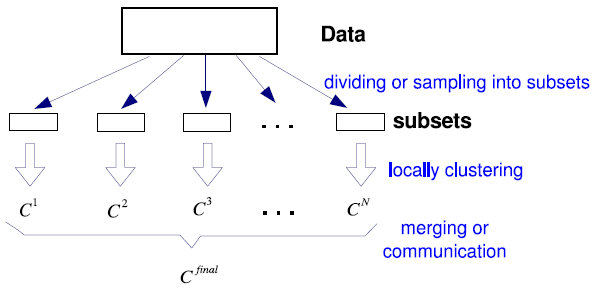
\includegraphics[width = 11 cm]{image/Chapters/Chapter3/divide.PNG}
%     \caption{Divide and conquer approach to generate clustering out of big data \protect\cite{zhang2009toward}}
%     \label{dividee}
% \end{figure}


% Our first attempt working with the extensive dataset was to implement this technique to generate data stream clustering \cite{ivarispatio}, and it was the first version of DSAP, which is presented in this thesis. However, it has a history of all data points, and the time and memory complexity are still high, and most algorithms that have this approach are unable to track the change in the trend of the data stream. 
% Due to the reason above, some research has been done on AP streaming clustering and introduce new approaches.

%##################################################### MOnica

In order to mimic a data stream, it was necessary to convert the collected data into a stream. For DSAP, this conversion was performed using the scikit-multiflow data stream simulation framework from Python.  Scikit-multiflow is a free and open-source tool and it is part of the River machine learning library in Python \cite{montiel2018scikit}. The prerequisites to install scikit-multiflow package (\textit{skmultiflow}) are NumPy and Cython libraries. 

The \texttt{skmultiflow.data} module includes two group of classes that either perform batch-to-stream conversions or generate standard data streams like waveform, Gaussian as shown in Figure \ref{sci}. The batch-to-stream conversion classes generates streams from a file source (.csv files) in the disk or from data in the memory.

\begin{figure}
    \centering
    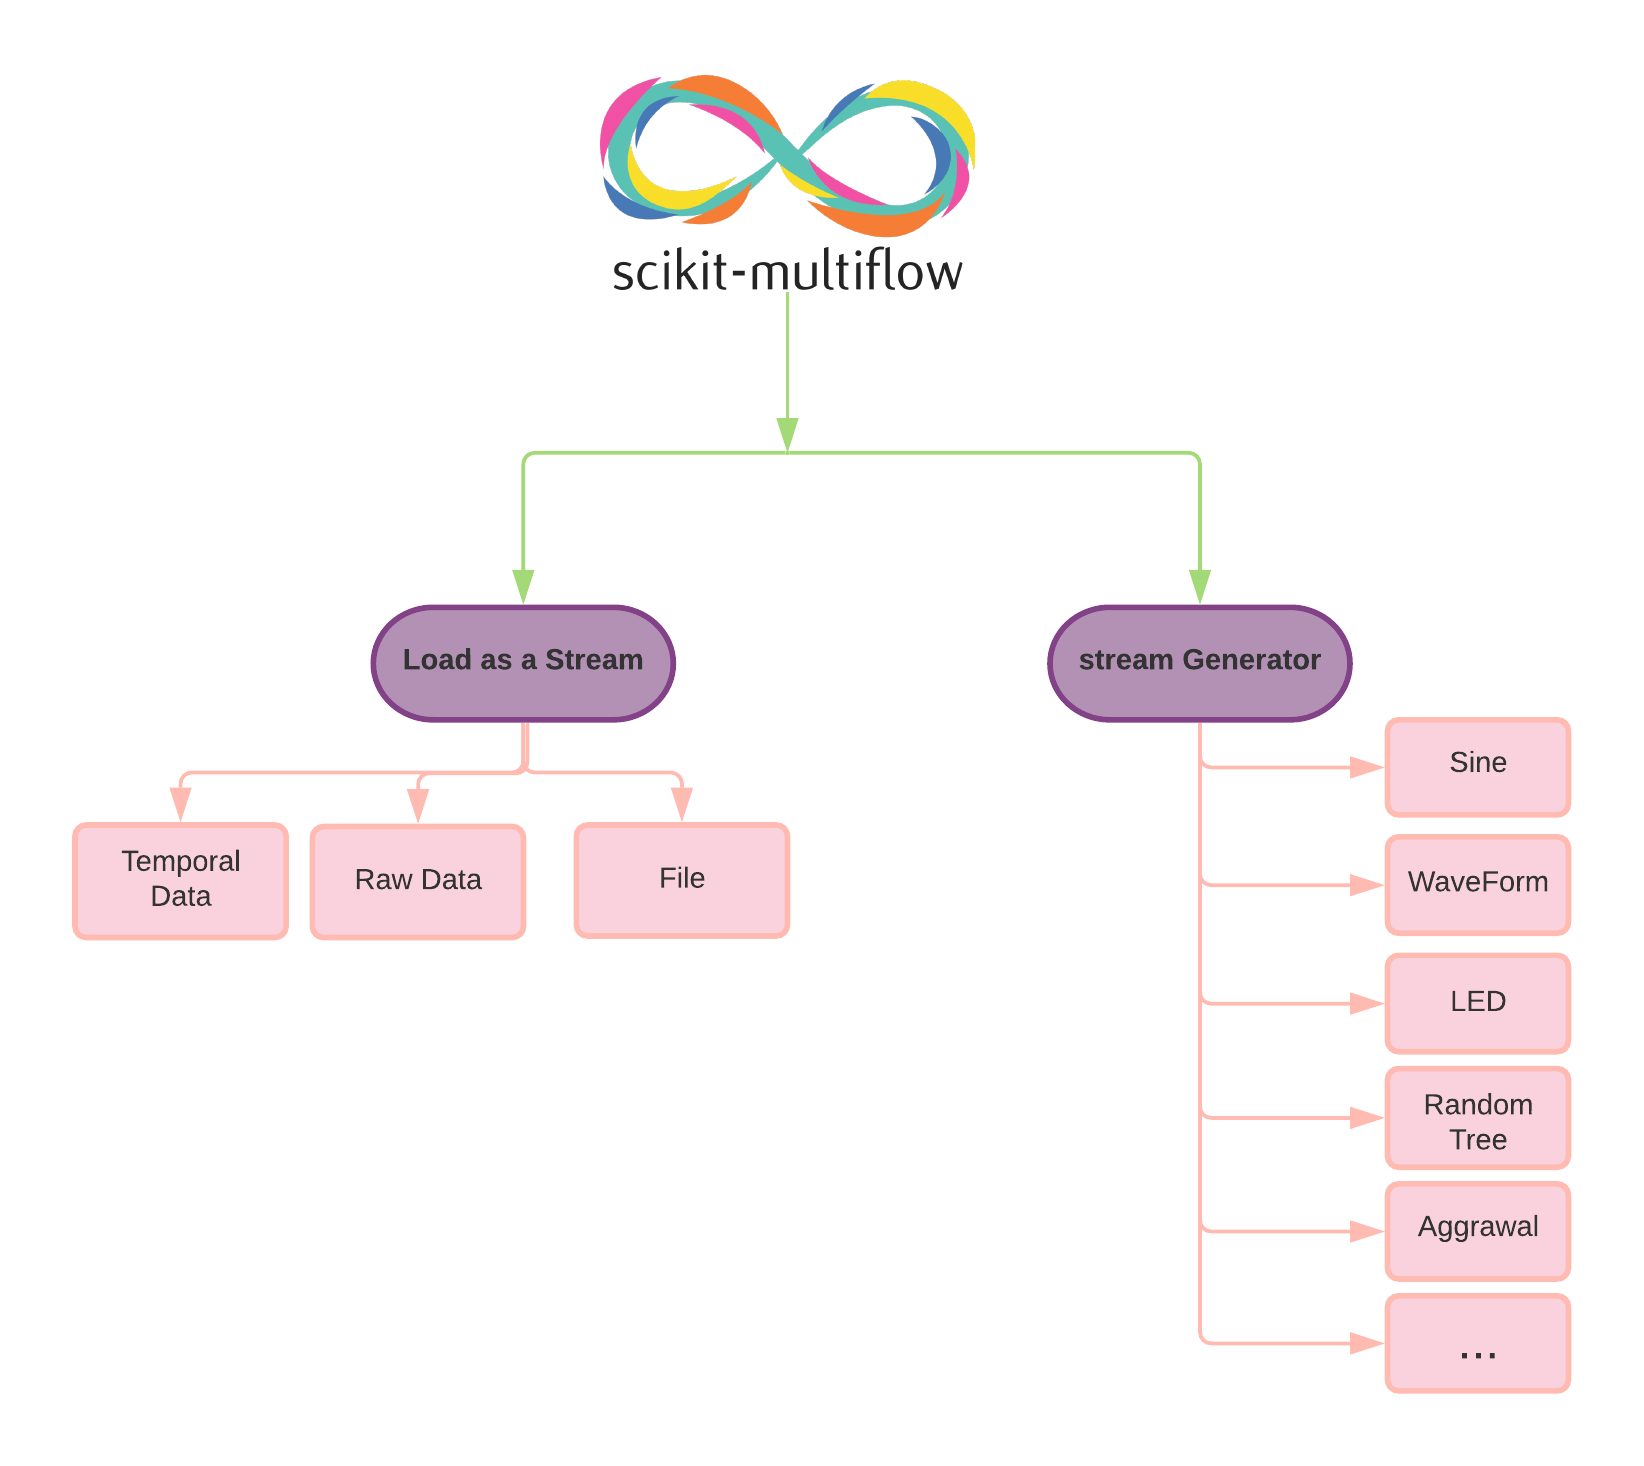
\includegraphics[width = 11 cm]{image/Chapters/Chapter5/multiflow.png}
    \caption{The scikit-multiflow data stream generator modules: load as a stream and stream generator}
    \label{sci}
    \end{figure}

The DSAP uses the \textit{skmultiflow.data.FileStream} class for generating data stream from any CSV file. It is part of the \texttt{skmultiflow.data} module and imported as: \texttt{skmultiflow.data.file\_stream}. Then, the data set is loaded as a stream (\texttt{ stream = FileStream (filepath)}), which is generated by the FileStream class. The Stream class is in charge of providing data inside scikit-multiflow and it runs upon request a number of samples, in a way such that old samples cannot be accessed at a later time. 

The most important method of the stream class is \texttt{next\_sample()}, which returns the next window at the start of every time interval. Also, the function \texttt{has\_more\_samples()} checks if any data point is left in the data set for consideration. Even though these packages are very capable of mimicking the data observed in data stream, the user still must acknowledge the limitations of such techniques. The difference from the real data stream can result from many potential shortcomings of the stream simulation models. The stream simulation packages do not have the support for generating realistic latency information, missing data, mixed timestamps, varying data cadence, and others. Hence any evaluation of the robustness and efficacy of a stream clustering algorithm done using the simulated streams should be cautiously accepted. 


\section{DSAP Clustering Phase}
%This section describes how the DSAP algorithm is implemented for data stream clustering using the landmark time window model in Python programming language. 

The DSAP source code in Python programming language has been made freely available at: \url{https://github.com/nasrineshraghi/DSAP}. The detailed description of each section of the code is presented below.

After the conversion of the CSV file data to a simulated stream, a landmark time window function \texttt{getWindowSize(start\_time, L)} is applied on the data points. This function finds the number of data points in a particular time window and returns this value. 

\begin{lstlisting}
# Estimate the number of data points within a time window
def getWindowSize(start_time,L):
    try:
        idx1 = np.where(df[:,2] >= start_time )[0][0]
        idx2 = np.where(df[:,2] >= start_time + L )[0][0] 
    except:
        idx1 = 0
        idx2 = 0
    XOmega = idx2 - idx1
# XOmega is window size
    windowSize = XOmega
    return windowSize
\end{lstlisting}


Every time window has a different start time, and this start time should be updated after the end of the window length is reached (\texttt{start\_time = start\_time + L}). If there is no data point available in a particular window or the number of them are few, the scikit-multiflow function (\texttt{stream.next\_sample(windowSize)}) skips that window and goes to the next one.

\begin{lstlisting}
from skmultiflow.data.file_stream import FileStream
# skip if the window is empty or few number of points are available
# For example 5 data points or less 
        if windowSize < 5:
            X = stream.next_sample()
            continue
        else:    
            j = j +1
\end{lstlisting}


It should be noted that if the landmark window is a count-based window instead of time, \texttt{windowSize} needs to be defined as the number of data point in each window instead of getting the value from the \texttt{getWindowSize} function above. For instance \texttt{windowSize = 100} means that each time the latest 100 data point from the stream are accessed. In this case number of data points in the window $\Omega$ is equal to $L$.

The DSAP online micro-cluster phase is implemented in three steps as described before in Chapter 4: initialization, comparison, and ActivateAP with update $\epsilon_{W_j}$.

In the Initialization step, the AP algorithm is applied on all data points present in the first window $W_0$ from the data stream. % (\texttt{AffinityPropagation().fit($W_0$)})

\begin{lstlisting}
#(1) Initialization. AP on the first time window
from sklearn.cluster import AffinityPropagation 
# AP library needs to be added first
preference = np.median(euclidean_distances(W0, squared=True))
AP = AffinityPropagation(preference, damping).fit(W0)
cluster_centers_indices = AP.cluster_centers_indices_
labels = AP.labels_
Cm = AP.cluster_centers_
n_clusters_ = len(cluster_centers_indices)
X = np.array(xi)
X_label = np.array(labels)
\end{lstlisting}

The AP algorithm generates a set of micro clusters ($C{_m}$). To initiate the DSAP model, a sufficient number of data points is required in the first window. Hence, it is important to choose an optimal value for the window size; otherwise, DSAP cannot reach convergence, and the model will fail. After the micro-clusters are generated, the distance matrix of all data points and centroids in each cluster are calculated by the \texttt{getAdaptiveThreshold()} function. The average distance of these values gives the initial $\epsilon_{W_0}$ that will be used in the comparison step.


\begin{lstlisting}
from scipy.spatial import distance
# Calculate the threshold distance
def getAdaptiveThreshold(Wj,Cm):
    epsilon = np.mean(distance.cdist(Wj,Cm,'Euclidean'))
    return epsilon 
\end{lstlisting}

In addition, the timestamp associated to each cluster centroids should be kept in an array with the size of initial centroids. The time for all centroids in the first window are equal.

\begin{lstlisting}
#time associated to initial centroids
tq = np.ones(len(Cm))*start_time
tq = tq.astype(int)
\end{lstlisting}


The output of the initialization step are a set of micro-clusters with centroids ($C_m$) and an initial threshold value ($\epsilon_{W_0}$).

The next step of the online micro-cluster phase is comparison. For the following windows from $W_1$ to $W_N$, all data points in each window are compared with the existing micro-clusters. The Euclidean distance of each new point $x_i$ in the window to its closest micro-cluster centroid is calculated. If the distance is less than the threshold $\epsilon_{W_j}$, $x_i$ is added to the micro-clusters and the timestamp associated to those specific centroids needs to be updated. Otherwise, it is kept temporarily in the time-window repository until all data points in the window are being evaluated. 

\begin{lstlisting}
#(2) Comparison step.
# Update the start time for each window
windowsize = getWindowSize(start_time, L)
start_time = start_time + L
indx = 0
repository = []
for i in range(windowSize):
    d = distance.cdist(Cm,x,'Euclidean')
    ind = np.argmin(d)    
    if min(d) < epsilon:
         X = np.concatenate((X , np.reshape(x[i,:],(-1,2))))
         X_label = np.concatenate((X_label , np.reshape(ind,(-1))))
         #Updating time associated to centroid met in this step
         tq[ind] = start_time
    else:
        repository.append(x[i])       
        indx = indx +1
\end{lstlisting}

%At the end, the AP will apply again to find new micro-clusters out of these data. If there is no data point is in the cache, the next window will come in the model.

In the next ActivateAP step, AP is applied on all the remaining data points in the time-window repository whose distance from the centroids are more than the adaptive threshold $\epsilon_{W_j}$ for the current time window. In the end, clusters obtained from this step are added to the updated micro-clusters.  


\begin{lstlisting}
#(3) ActivateAP step for the time-window repository points
repositorydata = np.array(repository)
preference = np.median(euclidean_distances(repositorydata, squared=True))
AP_crepository = AffinityPropagation(preference, damping).fit(crepositorydata)
C`m = AP_repository.cluster_centers_
AP_repository_label = AP_repository.labels_
X = np.concatenate((X , np.reshape(repositorydata[i,:],(-1,2))))
X_label = np.concatenate((X_label , np.reshape(AP_repository_label,(-1))))
#C`m is the Cm prime, new micro-clusters
Cm = np.append(C`m, Cm, axis = 0)
# Assign timestamp to new micro-clusters
repository_tq = np.ones(len(C`m))*start_time
repository_tq = repository_tq.astype(int)
tq = np.concatenate((tq, repository_tq), axis=0)
\end{lstlisting}


As new micro-clusters are generated at the end of the ActivateAP step, the threshold value needs to be recalculated based on the updated micro-clusters. Once again the adaptive threshold function is called upon to estimate new threshold values. This value is compared with the threshold $\epsilon_{W_j}$. If the value is greater than $\epsilon_{W_j}$ then a average of the two thresholds is selected as the new threshold otherwise the threshold remains unchanged. The decision to choose the average of the two numbers was taken to ensure that the threshold does not blow up in size due to a sparse cluster or noise.
\begin{lstlisting}
# Update the threshold value.
epsilonC`m = getAdaptiveThreshold(C`m, repositorydata)
if epsilon < epsilonC`m:
    epsilon = (epsilonC`m + epsilon)/2  
\end{lstlisting}

In order to keep the number of micro-clusters under control and avoid obsolete clusters, cluster centroids that are older than the expiration number $e_x$ times the time period (older than a specific number of landmark) are removed periodically. The oldest relevant time is calculated by subtracting the $e_x$ number of time periods from the current timestamp (\texttt{start\_time}). The centroids with timestamps greater than this value are retained in the updated centroids along with their updated associated timestamps. Based on the duration of interest this expiration value is set by the user at the start of the stream clustering process. 



\begin{lstlisting}
# Remove old micro-clusters
# Number is an integer value defines by the user
ex = int Number
remain_centers = np.ones(len(tq))
for i in range(len(tq)):
    # Remove the centroids with time more than the ex
    if tq[i] < start_time - ex * L:
        remain_centers[i] = 0
indx_remain= np.where(remain_centers==0) 
Cm  = Cm[remain_centers==1]
tq = tq[remain_centers==1]
a = indx_remain[0]
for j in range(len(a)):
    indx = np.where(X_label == a[j])
    # Remove the labels with time more than ex
    X_label= np.delete(X_label, indx)

\end{lstlisting}


The next phase of the DSAP algorithm is the offline macro-cluster phase which generates final clusters by applying the AP algorithm one more time to all the micro-cluster centroids accumulated during the online phase (\texttt{AffinityPropagation().fit ($Cm$)}). In the offline phase only the summary statistics represented by the micro-clusters centroids stored during the online phase is used and not the actual data set itself. The number of micro-clusters is a lot smaller than the total number of points in the data set that it represents. The number of macro-clusters obtained in this phase are less than the number of micro-clusters as they summarize the whole period of observation and not individual windows. The pseudo-code presented in Algorithm \ref{algSDAPi} shows the outline of the entire DSAP algorithm. 

\begin{lstlisting}
# Offline Macro-clustering Phase
preference = np.median(euclidean_distances(Cm, squared=True))
AP_mac = AffinityPropagation(preference, damping).fit(Cm)
cluster_centers_indices_mac = AP_mac.cluster_centers_indices_
cluster_centers_mac = AP_mac.cluster_centers_
mac_label = AP_mac.labels_

\end{lstlisting}


%\todo[inline]{ALGORITM HERE} 
%%%%%%%%%%%%%%%%%%%%% DSAP  %%%%%%%%%%%%%%%%%%%%%%%%%%%%%%%%%%

\begin{algorithm}[htbp]
       
\caption{DSAP Algorithm}
    \label{algSDAPi}
\small
    \textbf{Input:}
         Data stream: $S$ as windows ${ W_0,W_1, ..., W_N : W_j = x_1, ..., x_{\Omega}}$ with the length L, ex ;\newline 
    \textbf{Hyperparameters:}
        {Preference, Damping, $\epsilon_{W_j}$}\newline
        \textbf{Output:}
        Set of micro clusters with centroids $Cm= [Cm_1,Cm_2, ..., Cm_q]$,  set of macro clusters with centroids $C_M= [C_{M_1}, C_{M_2}, ...C_{M_k}]$ \\
        
        \SetKwFunction{FIROC}{getWindowSize} 
         \SetKwProg{Fn}{Function}{}{}
         \Fn{\FIROC{$start\_time, L$} 
         }{
         $time\_period = start\_time + L$ \\
         $windowSize$ = $S(time\_period)$
        %  $windowSize = time\_period - start\_time$
         }
         \KwResult{$windowSize$} 
                 \SetKwFunction{FIROC}{getAdaptiveThreshold}          
         \SetKwProg{Fn}{Function}{}{}
         \Fn{\FIROC{$W_j$, $Cm$}}{
         $\epsilon_{W_j}$ = mean(d($W_j, Cm$))
                  }
         \KwResult{$\epsilon_{W_j}$} 
         \Statex  \hfill              
         \ContinuedFloat\hfill
        \textcolor{red}{\textbf{Online Phase}}\\
         j = 0\\
         \While{!(stream.has\_more\_samples())}{
         
      	\eIf{(j == 1) %\tcp{\color{green}First window}
       	} 
       	{\hfill \Comment{Initialization}\\
       	$W_0$ = \texttt{S.getWindowSize($start\_time, L$)}\;\newline
       	\SetKwFunction{FIROC}{AP}        \;  
             \SetKwProg{Fn}{Function}{}{}
             \Fn{\FIROC{ $W_0$}}{}
             \KwResult{Initial micro-clusters: $Cm = [Cm_1,Cm_2,...,Cmq]$, label data points: $X$, $[tq] = start\_time$}\\
             $\epsilon_{W_j}$ = getAdaptiveThreshold($W_0, Cm$)\;
            
             }
             {
      $W_j$ = \texttt{S.getWindowSize($start\_time + L*j, L$)}\;\\
      $start\_time = start\_time + L$\\
       
              %  \If{getWindowSize == 0}
      %  {$W_j = W_j + 1$}  \newline
        % \newline
        
         %\Statex \hfill     \textbf{{Online Phase:}}\\
        \For{($x_i:i = 1:\Omega$)}{\hfill \Comment{Comparison}\;\\
        $[d]$ = d($[Cm], x_i$) \newline
        
        \eIf{min ($[d]) < \epsilon_{W_j}$}
        {   
        $Cm[X] \leftarrow{x_i}   $
        (merge with micro\_clusters)\\%\tcp{kkkk}\\
        $[tq] = start\_time$
        
        }
        {
        \STATE $repository \leftarrow{x_i} $ 
        
        %\STATE $W_i \xrightarrow \mathrm{C_{m0}}$\;
        }
        
        \hfill \Comment{ActivateAP}\\
        %if 1st
        %  \If{$i == \Omega$}
        %  {                                  
         \SetKwFunction{FIROC}{AP}          
         \SetKwProg{Fn}{Function}{}{}
         \Fn{\FIROC{repository}}{}
         \KwResult{new micro-clusters:$[C'm]$\\
                $\epsilon_{W_J}'$ = getAdaptiveThreshold($C'm,repository$)\\
                $tq_{repository} = start\_time$
                }

        %  }
        }

        Update micro\_clusters: $Cm = Cm + C'm$ \\
        Updated timestamp $tq = tq + tq_{repository}$\\
        Update Threshold : $\epsilon_{W_j}$
        
        

      }
       
      \If{$tq < start\_time - ex * L$}
        {Discard Cm }
         
        \textbf{Results: } Micro Clusters: $Cm= [Cm_1,Cm_2,Cm_3, ..., Cm_q]$ %}
        }
        \end{algorithm}
        \begin{algorithm}
            

         \If{end of S}{            \\            
          \ContinuedFloat\hfill
\textcolor{red}{\textbf{Offline Phase}}\\
         
         \SetKwFunction{FIROC}{AP}
         \SetKwProg{Fn}{Function}{:}{}
        \Fn{\FIROC{$Cm$}}{}
     \KwResult{Macro Clusters: $C_M= [C_{M_1}, C_{M_2}, ...C_{M_k}]$} 
     }

\end{algorithm}


%\section{Streaming K-means Algorithm}
% The established streaming K-means algorithm was chosen for comparison with the proposed DSAP algorithm. The variant of the algorithm for this study is part of the stream framework implemented in R programming language for data stream modeling and associated data mining tasks such as clustering and classification \cite{packager}. This version of the streaming K-means algorithm was chosen as the stream package not only provides an easy interface for k-means cluster computation, but also includes a lot of other popular clustering techniques that will aid in future model comparisons. Streaming-Kmeans has been successfully used to analyze data streams from wearable devices by our group at UNB using the same R package. 

% The R stream framework consists of two main components as shown in Figure \ref{streammm}:
% \begin{itemize}
%     \item Data Stream Data (DSD) object simulates the data stream.
%     \item Data Stream Clustering (DSC) task to find clusters out of a simulated data stream.
% \end{itemize}

% \begin{figure}[!h]
%     \centering
%     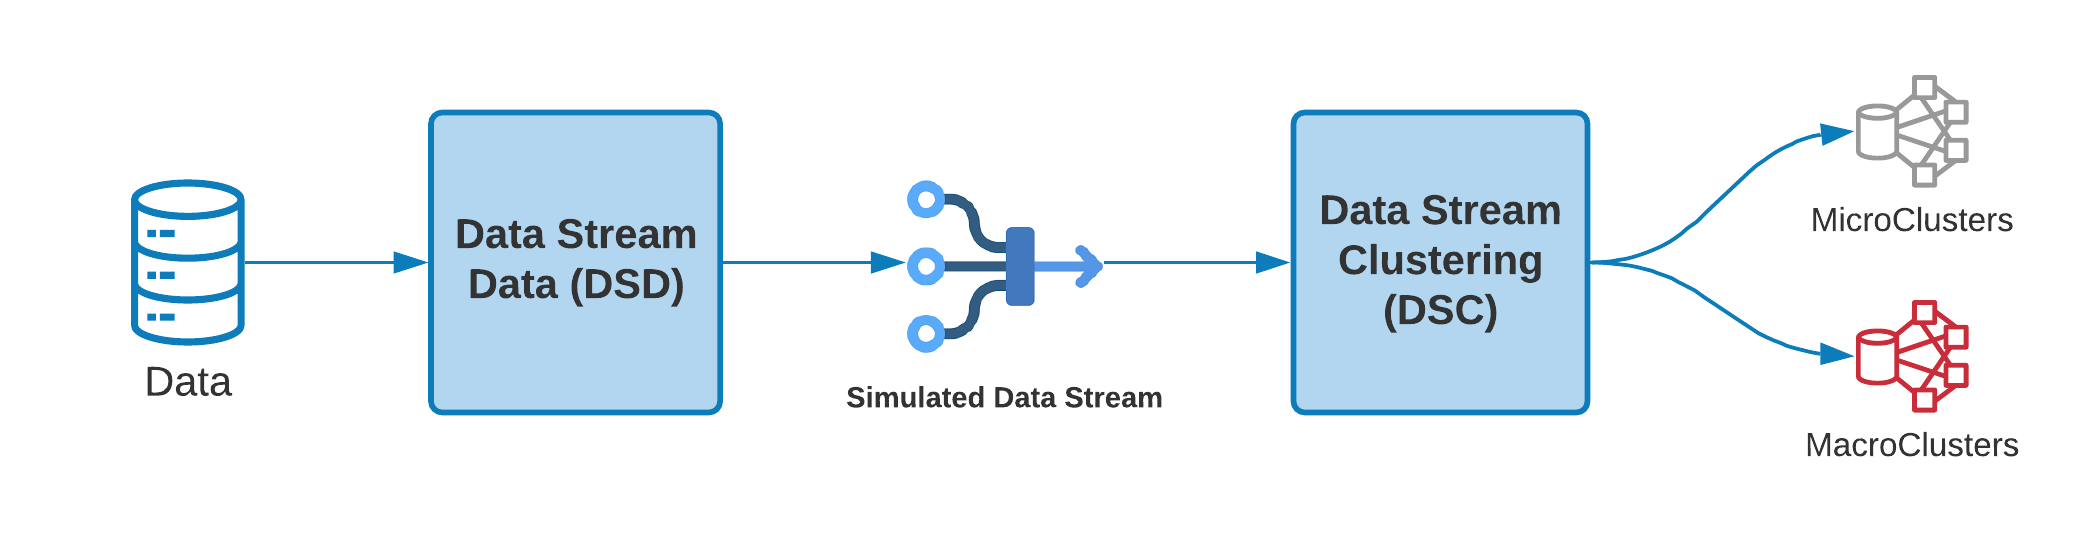
\includegraphics[width=.9\textwidth]{image/Chapters/Chapter5/RKmeans.png}
%     \caption{ Data stream simulation with R stream framework. This part is called DSD, has tree modules.}
%     \label{streammm}
% \end{figure}




% % Overview of R framework for streaming K-means with two steps: the data stream Data (DSD) and data stream clustering (DSC) class structure.    
    
% \subsection{Data Stream Simulation}
% %  All these modules are presented in the \texttt{Stream} package.
% The Data Stream Data (DSD) object which is part of the \texttt{Stream} package is an abstraction layer that connects to any streaming data source. The stream package provides several DSD implementations as shown in Figure \ref{dsd}. The simulated stream generated by the DSD can mimic static streams as well as streams with concept drift. In-flight implementation can be used to standardize in terms of centering and scaling data in a data stream. % in-flight.  
% Read data connector class provides simulated streams in three different ways: \texttt{DSD\_Memory}, gives streaming interface to data in memory which represents a part of data, \texttt{DSD\_ReadDB} provides an interface from SQL query to the database, and \texttt{DSD\_ReadCSV} reads data line by line from a file or a connection and makes it available in a streaming manner. This enables a system to process data that is larger than the available memory. Connections to real data can be applied to read from real-time data streams.

% \begin{figure}[!htb]
%     \centering
%     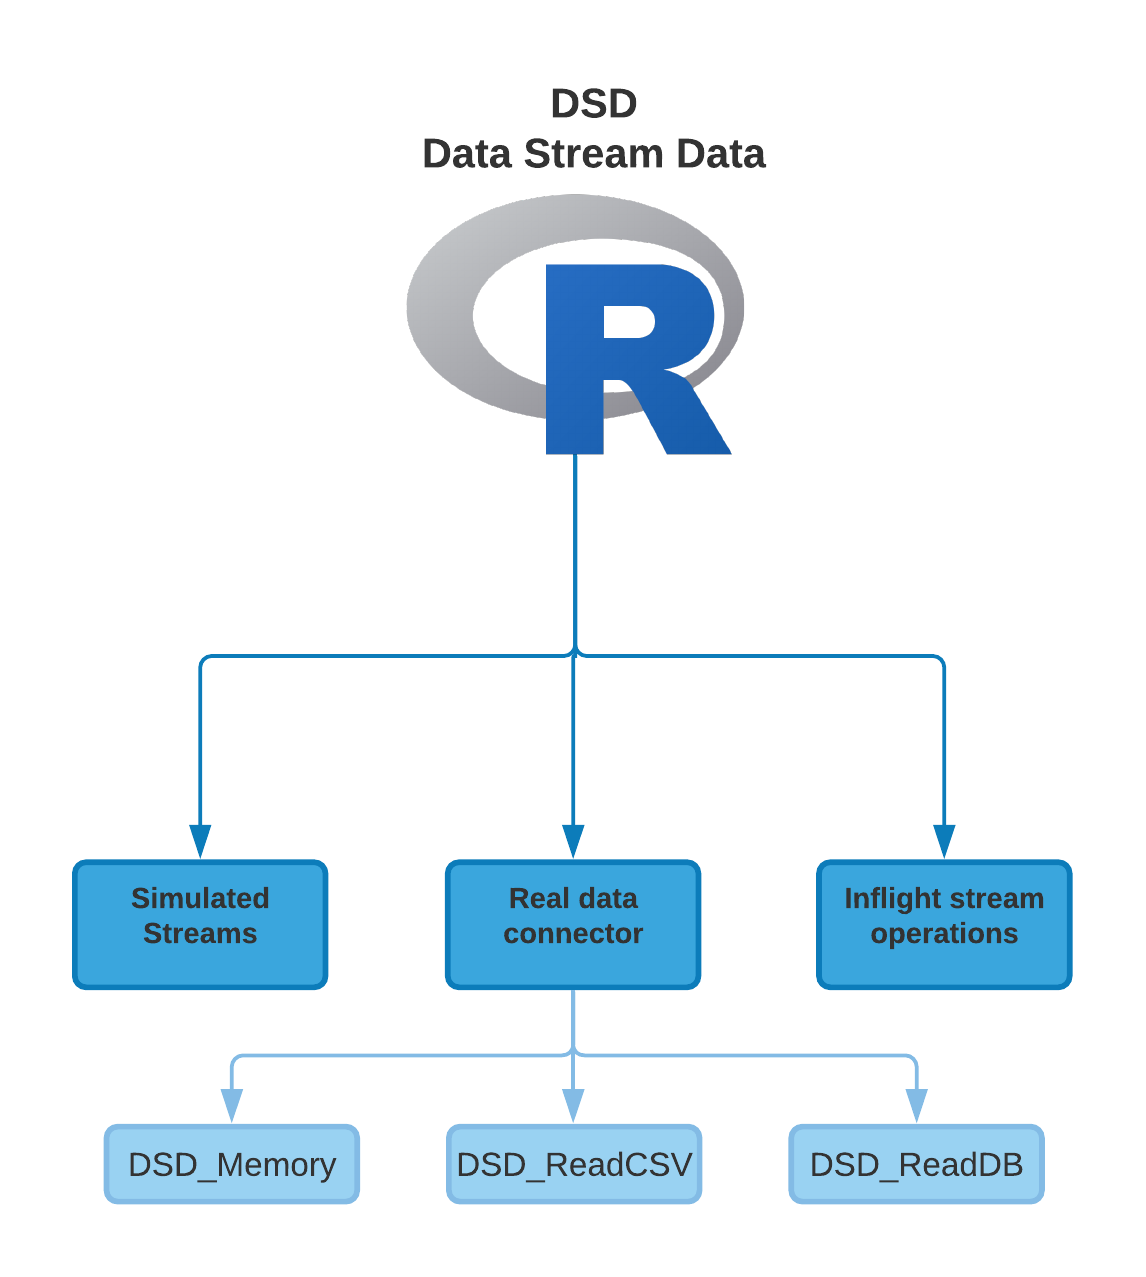
\includegraphics[width = 8 cm]{image/Chapters/Chapter5/dsd.png}
%     \caption{ .}
%     \label{dsd}
% \end{figure}


% To generate data stream out of the CSV files, \texttt{DSD\_ReadCSV()} class is used. This class has some unique features such as the ability to change position in the file and reset it to the beginning and the connection can be closed anytime. All the DSD packages have the same interface using the two functions: a creator function whose outcome is not a dataset but an object describing the stream's properties and its current state, and a data generating function like \texttt{get\_point()} that is handled to get the next data point from the stream.

% % \begin{lstlisting}
% #reading the data out of file
% stream <- DSD_ReadCSV(file, loop=FALSE, sep=",", header=FALSE, ...)
% \end{lstlisting}

% \subsection{Data Stream Clustering}
% After applying a DSD class to generate the data stream, the next step is to analyze the data stream to generate clusters. The Data Stream Clustering (DSC) object in the stream package provides multiple options to analyze the data as shown in Figure \ref{dsc}. The two stage \texttt{DSC\_TwoStage} clustering framework was chosen for this study. It combines two abstract classes that create micro-clusters \texttt{DSC\_Micro} and macro-clusters\texttt{DSC\_Macro}.
% % \begin{lstlisting}
% # create a clustering process that uses a window for the online and k-means for the offline phase 
% win_km <- DSC_TwoStage(
%   micro = DSC_Window(horizon, lambda),
%   macro = DSC_Kmeans(k)
%   )
% win_km
% update(win_km, stream, 200)
% \end{lstlisting}
% As shown in the above code, the 
% The two classes in \texttt{DSC\_TwoStage} which form the core of the streaming K-means clustering algorithm are: 

%     \begin{itemize}
%         \item\texttt{DSC\_Window():} provides a clustering interface to the data stream operator. It implements a window model, which keeps a specified number of data points from the stream in a format defined by the user. This number is the window length. 
        
%         \item\texttt{DSC\_Kmeans():} class implements the R version of the k-means algorithm for reclustering a set of micro-clusters. In this version of k-means the data points (micro-clusters) can be weighted based on the micro cluster density. The streaming k-means clustering algorithm requires a continuously updated set of micro clusters.

%     \end{itemize}


% This algorithm is capable of handling data as sliding or damped time windows that are generated by the \texttt{DSC\_Window()} class. For the sliding time window a user-specified number (window length) of the most recent data points of the stream are kept as the micro-cluster. For the damped window model, data points in the window have a weight that deceases exponentially with age. \texttt{DSC\_Window()} can also generate and analyze hopping/landmark time window model as this is just a special case of the sliding time window when there is no overlap in sliding window. In the macro-cluster step the K-means algorithm needs to be provided with the number of clusters parameter $k$. This parameter is set by applying elbow method that was discussed earlier in section \ref{kmeansalgo}. Ideally this parameter should be automatically estimated but due to the small datasets analyzed for this study this wasn't deemed necessary and hence the $k$ value was calculated separately.

% \begin{figure}[]
%     \centering
%     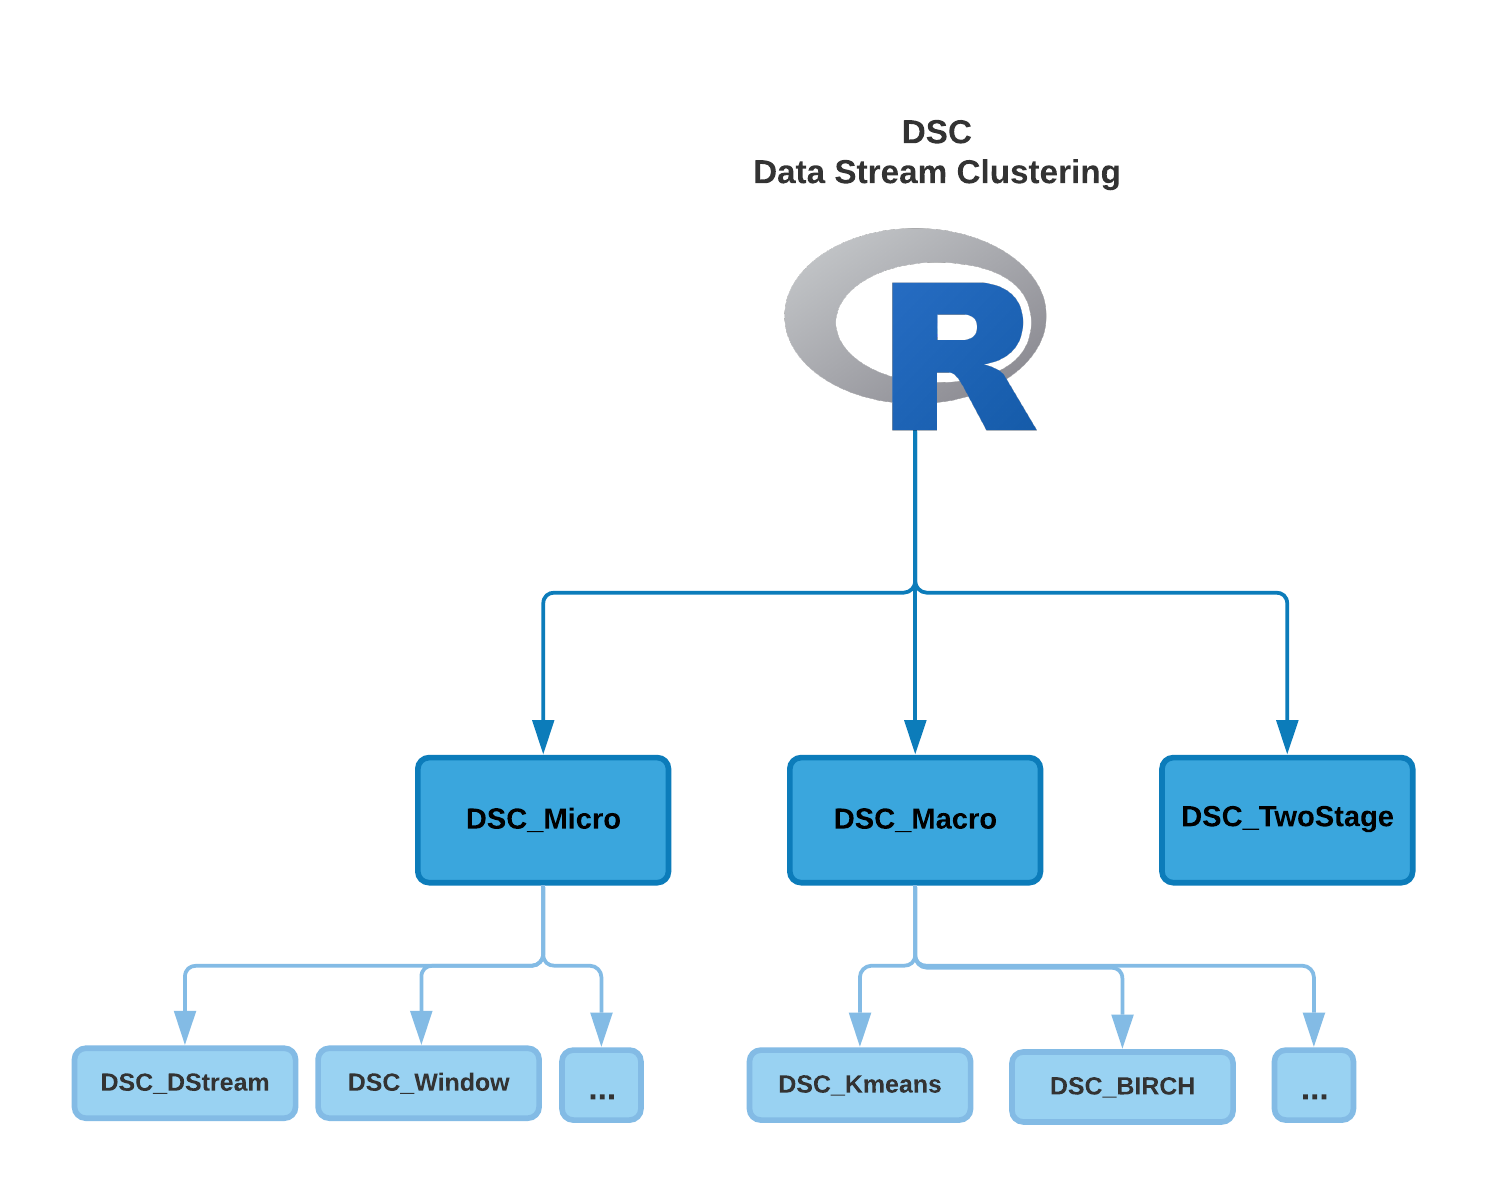
\includegraphics[width=.7\textwidth]{image/Chapters/Chapter5/DSC_all.png}
%     \caption{ .}
%     \label{dsc}
% \end{figure}



\section{Intrinsic Clustering Validation Phase}
To validate the clustering results, three Intrinsic evaluation metrics: Silhouette Coefficient, Caliński-Harabasz Index, and Davies-Bouldin Index, are used as discussed earlier in section \ref{intrinval}. All the three metrics were implemented in Python.  

%for both the DSAP and the streaming K-means algorithms that were implemented in Python and R programming language  respectively. Standard functions are available for each of the metrics in both the programming languages. These metrics are one way to evaluate the quality of clustering and compare our work with the existing streaming K-means.


\begin{itemize}
    

\item\textit{Silhouette Coefficient}
Silhouette Coefficient cluster evaluation metric was implemented as a function \texttt{silhouette\_score} and is available in the \texttt{sklearn.metrics} library in Python.  The input parameter of this function is an array of pairwise Euclidean distances between micro-cluster centroids and the final macro-cluster centroids, %cluster label for each data point, and metric to use for calculating a distance between data points in a feature array which is Euclidean for our work. 

%The Silhoutte calculation in R is performed by the function \texttt{silhouette()} that is available in package \texttt{cluster}. This function \texttt{silhouette(distdata, idmedoid, idcluster)} just needs a vector of cluster members and a dissimilarity matrix.




\item\textit{Caliński-Harabasz Index}
It is available in the \texttt{sklearn.metrics} library of Python as the \texttt{calinski\_harabasz\_score} function. The input parameter of this metric is a list of $n\_$features-dimensional data points in which each row corresponds to a single data point and labels related to each data. The output of this function is a float number with no cut-off value. The higher the value, the "better" is the solution.

%The implementation of this metric in R is part of the \texttt{cluster.stats} library and is used for cluster validation. The function is called: \texttt{calinhara(x, clustering, cn= max(clustering))}, where $x$ is the data frame, clustering is a method of implementation, and $cn$ is the number of clusters.



\item\textit{Davies-Bouldin Index}
The last metric is the Davies-Bouldin Index that was implemented in Python as part of the same library \texttt{sklearn.metrics} as CHI. The function which is called \texttt{davies\_bouldin\_score} has two input parameters: list of $n\_$features-dimensional data points and labels. This result is a float number whose lower values indicate tighter clusters that are better separated.


%This metric is a part of \texttt{clusterSim} library in R. The function is called: \texttt{index.DB(x, cl, d=NULL, centrotypes="centroids", p=2) }, where $x$ is a data frame, $cl$ is vector of integer numbers showing the cluster to which each data point is allocated, $d$ is an optional distance matrix, and $p$ is the power of the Minkowski distance between centroids of clusters: p=1 - Manhattan distance; p=2 - Euclidean distance.


\end{itemize}


\section{Clustering Performance Evaluation Phase}
Analogous to the intrinsic cluster validation phase where the quality of the clusters was assessed, in this phase the DSAP algorithm is evaluated in terms of computational time efficiency and memory consumption. Straightforward functions are available in both Python to compute these two metrics. 
\begin{itemize}
    \item \textit{Processing Time:} To find the running time in Python, the time function within the \texttt{time()} module is used to get the execution time of the algorithm. This module calculates the running time of a program by first storing the starting time and ending time, before the first and after the last line. At the end, the difference between these two times would be the total running time of the program. The time() function returns the number of seconds elapsed since the epoch.

    \item \textit{Memory Consumption:} To monitor memory usage, the \texttt{os} and \texttt{psutil} libraries in Python are used. Psutil (Python system and process utilities) is a cross-platform library for retrieving information on running processes and system utilization (CPU, memory, disks, network, sensors). \texttt{psutil.virtual\_memory()} function returns statistics about system memory usage. Also, Python provides a C module called cProfile, which provides deterministic profiling of Python programs. A profile is a set of statistics that describes how often and for how long various parts of the program are executed. This module is mainly used when we wanted to calculate the window length and threshold. 
    %The \texttt{memory.size()} function displays the amount of memory consumed by the R program. The \texttt{mem\_change()} captures the net change in memory when running a code. These functions can be used to estimate how much memory is consumed by  

% memory\_info()
% Return a named tuple with variable fields depending on the platform representing memory information about the process. The “portable” fields available on all platforms are rss and vms. All numbers are expressed in by


\end{itemize}



% This package provides simulated streams in three different ways: static structure, concept drift, or connectors to real data and streams. The static structure is used for simulating the random Gaussian, bench, and noise data stream. The concept drift is applied to generate a specific complex of a data stream with this concept. Connectors to real data DSD object has three categories as explained below.

% \begin{itemize}
%     \item\textbf{DSD\_Memory:} It gives a streaming interface to the matrix, static data in memory, representing a fixed portion of a data stream. Also, DSD\_Memory can generate a copy of a part of another DSD object to be replayed in experiments many times.
    
%     \item\textbf{DSD\_ReadCSV:}  It reads data line by line from a file or a connection and makes it available in a streaming manner. Then, it enables a system to process data that is larger than the available memory. Connections to real data can be applied to read from real-time data streams.
    
%     \item\textbf{DSD\_ReadDB:} KINI presents an interface to result set from a SQL query to any other relational database.  These databases can use the DBI interface. 
% \end{itemize}

%All the DSD packages have the same interface using the two functions: a creator function whose outcome is not a dataset but an object describing the stream's properties and its current state, and a data generating function that is handled to get the next data point from them stream represented by object k.

    % \item\textbf{DSC-based clustering:} The simulated data stream generated by the DSD object described experiment is calculated in two phases by the \textit{'stream'} package under the \textit{Two\_Stage} framework. Stream includes a special Data Stream Clustering (DSC) class called \textit{DSC\_TwoStage}, which combines \textit{DSC\_Micro} and \textit{DSC\_Macro} K-means into a two-stage online and offline process by applying time window models.
    % In data stream clustering (DSC) phase, stream currently provides moving windows and sampling from a stream as data stream operators. DSC\_Window provides a clustering interface to the data stream. It implements the sliding window, landmark and the dampened window models which keep a user-specified number (window length) of the most recent data points of the stream. For the dampened window model, data points in the window have a weight that deceases exponentially with age.
    % This function, call two sub-function:
    %   % make sure!
    % \begin{itemize}
    %     \item\texttt{DSC\_Window():} provides a clustering interface to the data stream operator $DSC\_Window$. It implements the window model, which keeps a specified number of the most recent data points of the stream defines by the user. This number is the window length. 
        
    %     \item\texttt{DSC\_Kmeans():} interface is the R version of K-means clustering implementation and a version of k-means where the data points (micro-clusters) are weighted by the micro cluster weights. The streaming k-means clustering algorithm requires continuously update the calculation of micro clusters.

    % \end{itemize}
    



%Simulation pack: Although the above two packages are very capable of mimicking the data observed in data stream, but the user must acknowledge the limitations of such techniques. The difference from the real data stream can result from many potential shortcomings of the stream simulation models. The stream simulation packages do not have the support for generating realistic latency information, missing data, mixed timestamps, varying data cadence, and others. Hence any verification of the robustness and efficacy or benchmarking of a stream clustering algorithm done using the simulated streams should be cautiously accepted. 

%The next sections explain how the workflow phases discussed earlier are implemented on indoor positioning and occupancy datasets. 
% \end{itemize}



%\section{Case studies}
%\todo[list]{section from chpater 2 moved here}

%\section{Indoor Localization  and Occupancy Detection}

% Location-based services (LBS) have become extremely popular, and it is part of daily life. The location-based services and their applications require a high level of standard in positioning technology. The positioning technology has shifted from the outdoors to the indoor, and this is because of two reasons \cite{xia2017indoor}. People usually spend most of their time indoors. Besides, most mobile phones and data communications are performed indoors. Moreover, phone data show that the demand for indoor mobile communication is very powerful. 

%Indoor localization systems can hire a wide range of technologies such as infrared, RFID, sensors, WiFi, Bluetooth, etc. Using WiFi is one of the best approaches due to the availability of mobile devices on the user side. 

% \begin{table}[]
% \caption{Comparison between GPS and WiFi technologies.}
% \small
% \centering
% \label{tab:my-table}
% \begin{tabular}{@{}ccc@{}}
% \toprule
% \textbf{Technology} & \textbf{Accuracy level} & \textbf{Advantage}                                                                                    \\ \midrule
% GPS                 & High                    & \begin{tabular}[c]{@{}c@{}}*Good accuracy\\ *Not strong for indoor\end{tabular}                       \\ \midrule
% WiFi                & Medium                  & \begin{tabular}[c]{@{}c@{}}*Good accuracy for indoor\\ *Limited coverage\\  *Medium cost\end{tabular} \\ \bottomrule
% \end{tabular}
% \end{table}


% The most used method for estimating the location of indoor mobile objects or positioning with WiFi networks is fingerprinting method. The fingerprinting method works based on signal strength. 

% \subsection{Indoor Localization Using People-counter Sensors}
% The magnificent growth of indoor localization studies can lead to many real-world applications, including smart homes, smart campuses, and localize users to provide services. The purpose of indoor localization is to recognize a location within a multi-storied building with a smart device.  The GPS does not work in an indoor environment accurately as signal strength fluctuates weakly, leading to the user’s device not receiving location updates at fixed periods. 

% There are various applications for measuring the number of people and occupancy, and it can be a simple pen and paper to fully automated sensor solutions.
% Automated solutions use people counting technology to automatically count people as they enter and exit buildings. People counting is ideal for any kind of buildings that requires an intelligent system, especially for huge and crowded buildings such as malls, hospitals, stadiums, etc. People's movement is precious data for occupancy monitoring, smart building management, and social distancing management.  Using these systems can give users a better understanding of the workplace and room usage, reduce energy consumption or optimize building design and staff levels.

% This technology can be considered in terms of:
% \begin{itemize}
%     \item\textbf{Accuracy}: Sensors are designed to count a number of people at any place continuously.
%     \item\textbf{Historical data log}: comprehensive historical data and reports are available with the user requests. Some reports may show how occupancy changes over time, also, how well the building complied with occupancy limits.
%     \item\textbf{Cost}: The cost of these sensors may be higher at first for the sensor hardware. However, this is offset by zero or minimal ongoing costs.
% \end{itemize}

% The bidirectional people counter sensors are one of these types of sensors used for the dataset applied in this research work. The principle of these sensors is based on the interruption of the horizontal infrared beans, which are usually installed at the entrance or exit. However, other technologies such as thermal and stereo-vision can be used. When this infrared beam is interrupted, the receiver detects this movement, increasing the internal counter. The sensor data will find its way to the server through the gateway SNG. The overview of this scenario shows in Figure \ref{people}. Different types of these sensors are available below, which are produced by the International Road Dynamics company.

% \begin{figure}
% \centering
% 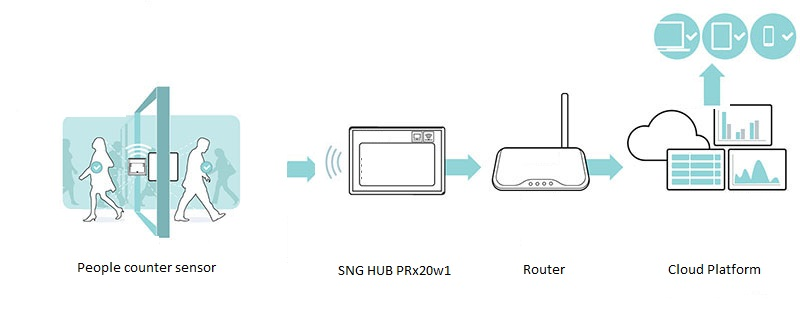
\includegraphics[width = 12cm,height = 5cm]{image/pc.jpg}
% \caption{People counter infrastructure used for our experimental dataset. Modified Figure of \protect\cite{SensM}}
% \label{people}
% \end{figure}


% \begin{table}[!h]{}
% \small
% \centering
% \caption{List of people counter sensors of International Road Dynamics company}%\cite{people}.}
% \begin{tabular}{llll}
% \toprule
% \textbf{Features} & \textbf{Transmitter} & \textbf{Receiver}  & \textbf{Applications}     \\
% \midrule
% Display/Wireless/Bidirectional     &  PTx20-1 & PRx20WD1 & Entrance and daily counts\\ 
% Wireless/Bidirectional             &  PTx20-1 & PRx20W1  & Entrance and daily counts\\ 
% Display/Bidirectional              &  PTx20-1 & PRx20D1  & Entrance and daily counts\\ 
% USB/Bidirectional                  &  PTx20-1 & PRx20U2  & Entrance and daily counts\\ 
% Display/USB/Bidirectional          &  PTx20-1 & PRx20UD2 & Entrance and daily counts\\ 
% \bottomrule
% \label{sensor}
% \end{tabular}
% \end{table}




% \subsection{Indoor Localization Using WiFi}

% Automatic user localization calculates the position of the user by knowing latitude, longitude, and altitude. This can be calculated by having an electronic device such as a mobile phone. Indoor localization is still a challenging topic, and it is because of the loss of GPS signals in indoor environments.

% Wireless-based indoor localization is another way for measurements. Wireless waves can go through obstacles like walls or doors and provide ubiquitous coverage of a building. WLAN indoor localization uses received signals value (RSSI) to indicate the distance to points and get the current point's location.
% This architecture needs two things, the beacon station that emits the wireless signals and electronic devices such as cellphones. 
% Fingerprint means the characteristic or feature of signals which RSS can be one of them. The assumption underneath this fingerprint-based indoor localization is that for each position in the area, the signals' features are different. By relying on the variation of signals in a distinct position, the current location can be obtained.



% ############################
% Two datasets that were obtained from short duration experiments lasting from a few days to a few months are analyzed in this thesis. The two experiments are the e-counter Indoor occupancy behavioural tests and the WiFi fingerprint Indoor Localization database. 
% Two case studies have been selected to evaluate the performance of the novel DSAP algorithm in a real-world scenario. Both the datasets analyzed in this work were part of short duration experiments lasting from a few days to a few months. 

% One method thought to increase incidental physical activity at work is the use of stair-promoting interventions. Stairs are readily available and stair climbing is considered vigorous physical activity. Motivational signs have been extensively and effectively trialled to increase stair use, but are they suitable for contemporary populations


%\subsection{E-counter Indoor Localization}

\section{Behavioural Intervention Experiment}

%Climbing stairs is an easy activity with proven health benefits which can be incorporated constructively in the lives of most people. 

Our first case study consists of an experiment performed in the Tonsley building at the campus of Flinders University, Australia in 2019. This study was conducted to observe the potential impact of motivational and educational interventions on the physical activity of people with sedentary lifestyles. 

% As part of the experiment, the number of people using stairs in the Tonsley building was monitored to study the stairs usage patterns. Nearly continuous measurements using e-counters were made over three months to infer any potential improvement in the stair usage after the introduction of motivational interventions. This included a month of undisturbed baseline measurements, a month of motivational intervention to increase stair use, and finally a month to observe the long term effect if any due to the intervention period. 





%The e-counter dataset used in this research was obtained from a behavioral intervention experiment to increase stair use that was The details of this experiment conducted in 2019 is described below.


%\subsubsection{Experiment}
 

%\begin{itemize}

% \item\textbf{Data Collection: }
%This experiment was conducted in the Tonsley Building over three months, that included a month of undisturbed baseline measurements, a month of motivational intervention to increase stair use, and finally a month to observe the long term effect if any due to the intervention period. 

Tonsley Building is a six-story building populated by students and staff with entrances facing North and South directions. The building floor layouts are illustrated in Figure \ref{laay}. The north-side entrance faces a small barricaded entrance as seen in panel \ref{laay:tpleft1}, but the main entrance is on the south side adjacent to the covered Tonsley garden. The building is fitted with lifts that reach all the levels, but also have stairs on the north and south sides that connect all the levels. Additionally, the building has an open space called the void and has central stairs that connect all the levels. Thus each level stairs are labeled as level $L_{x+1}-L_x$ North/South/Central, where $L_x = 1,2,.5$. 


\begin{figure*}[ht]
\centering
\subfloat[Google View of the building]{\label{laay:tpleft1}{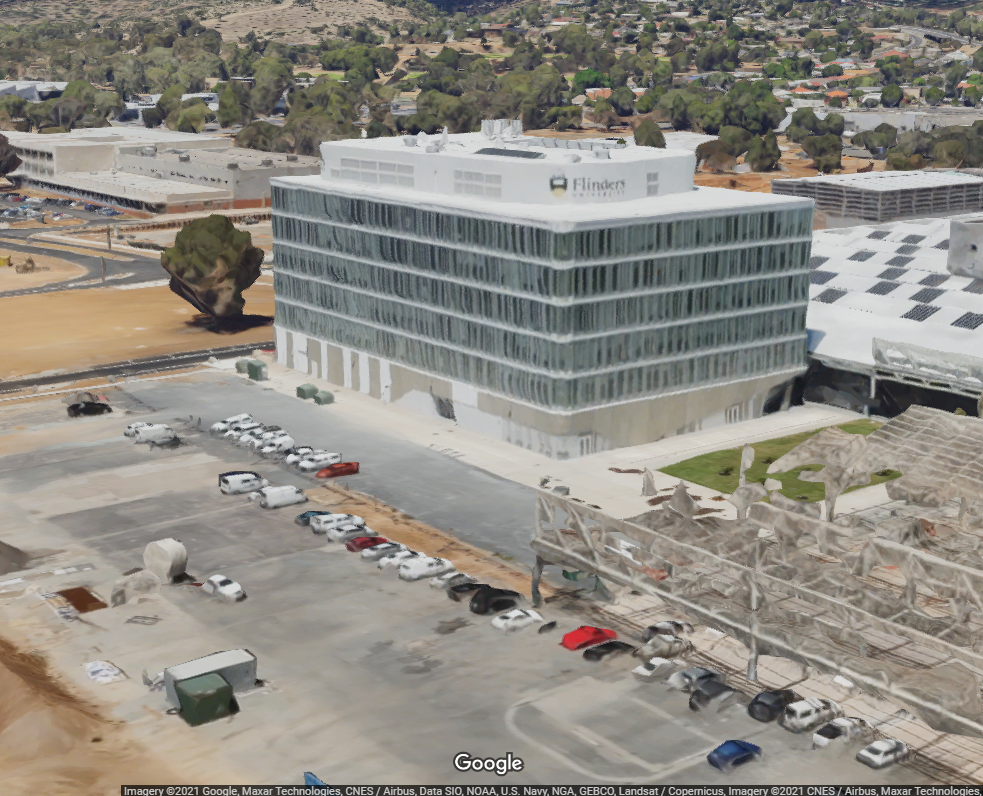
\includegraphics[width=5 cm, height = 4.2 cm]{image/Chapters/Chapter5/flinder.PNG}}}\hfill
\subfloat[Level 1]{\label{fig:md}{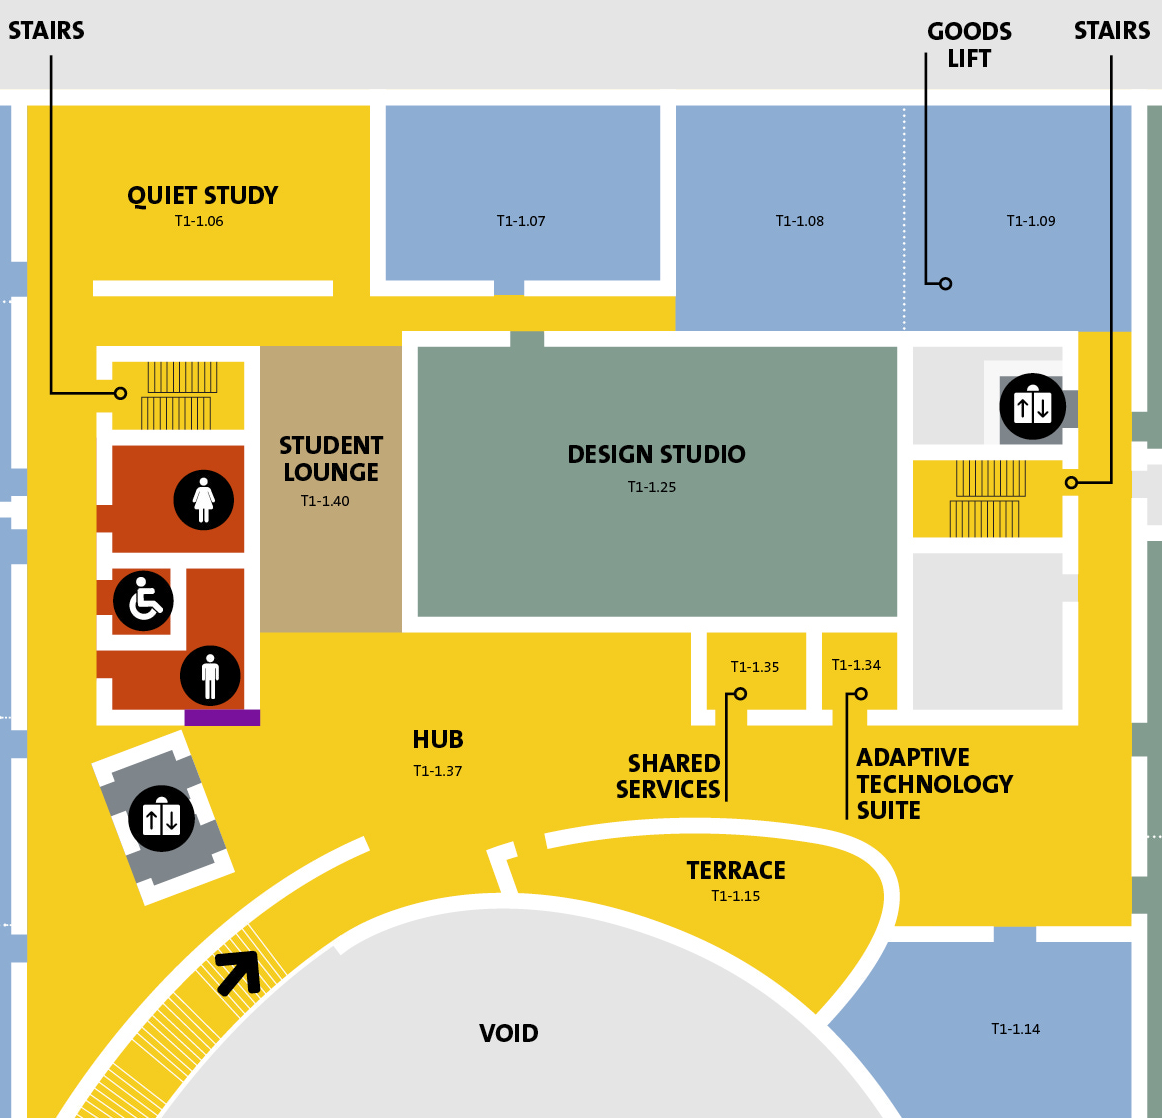
\includegraphics[width=0.3\textwidth]{image/T1.png}}}\hfill
\subfloat[Level 2]{\label{fig:mdright}{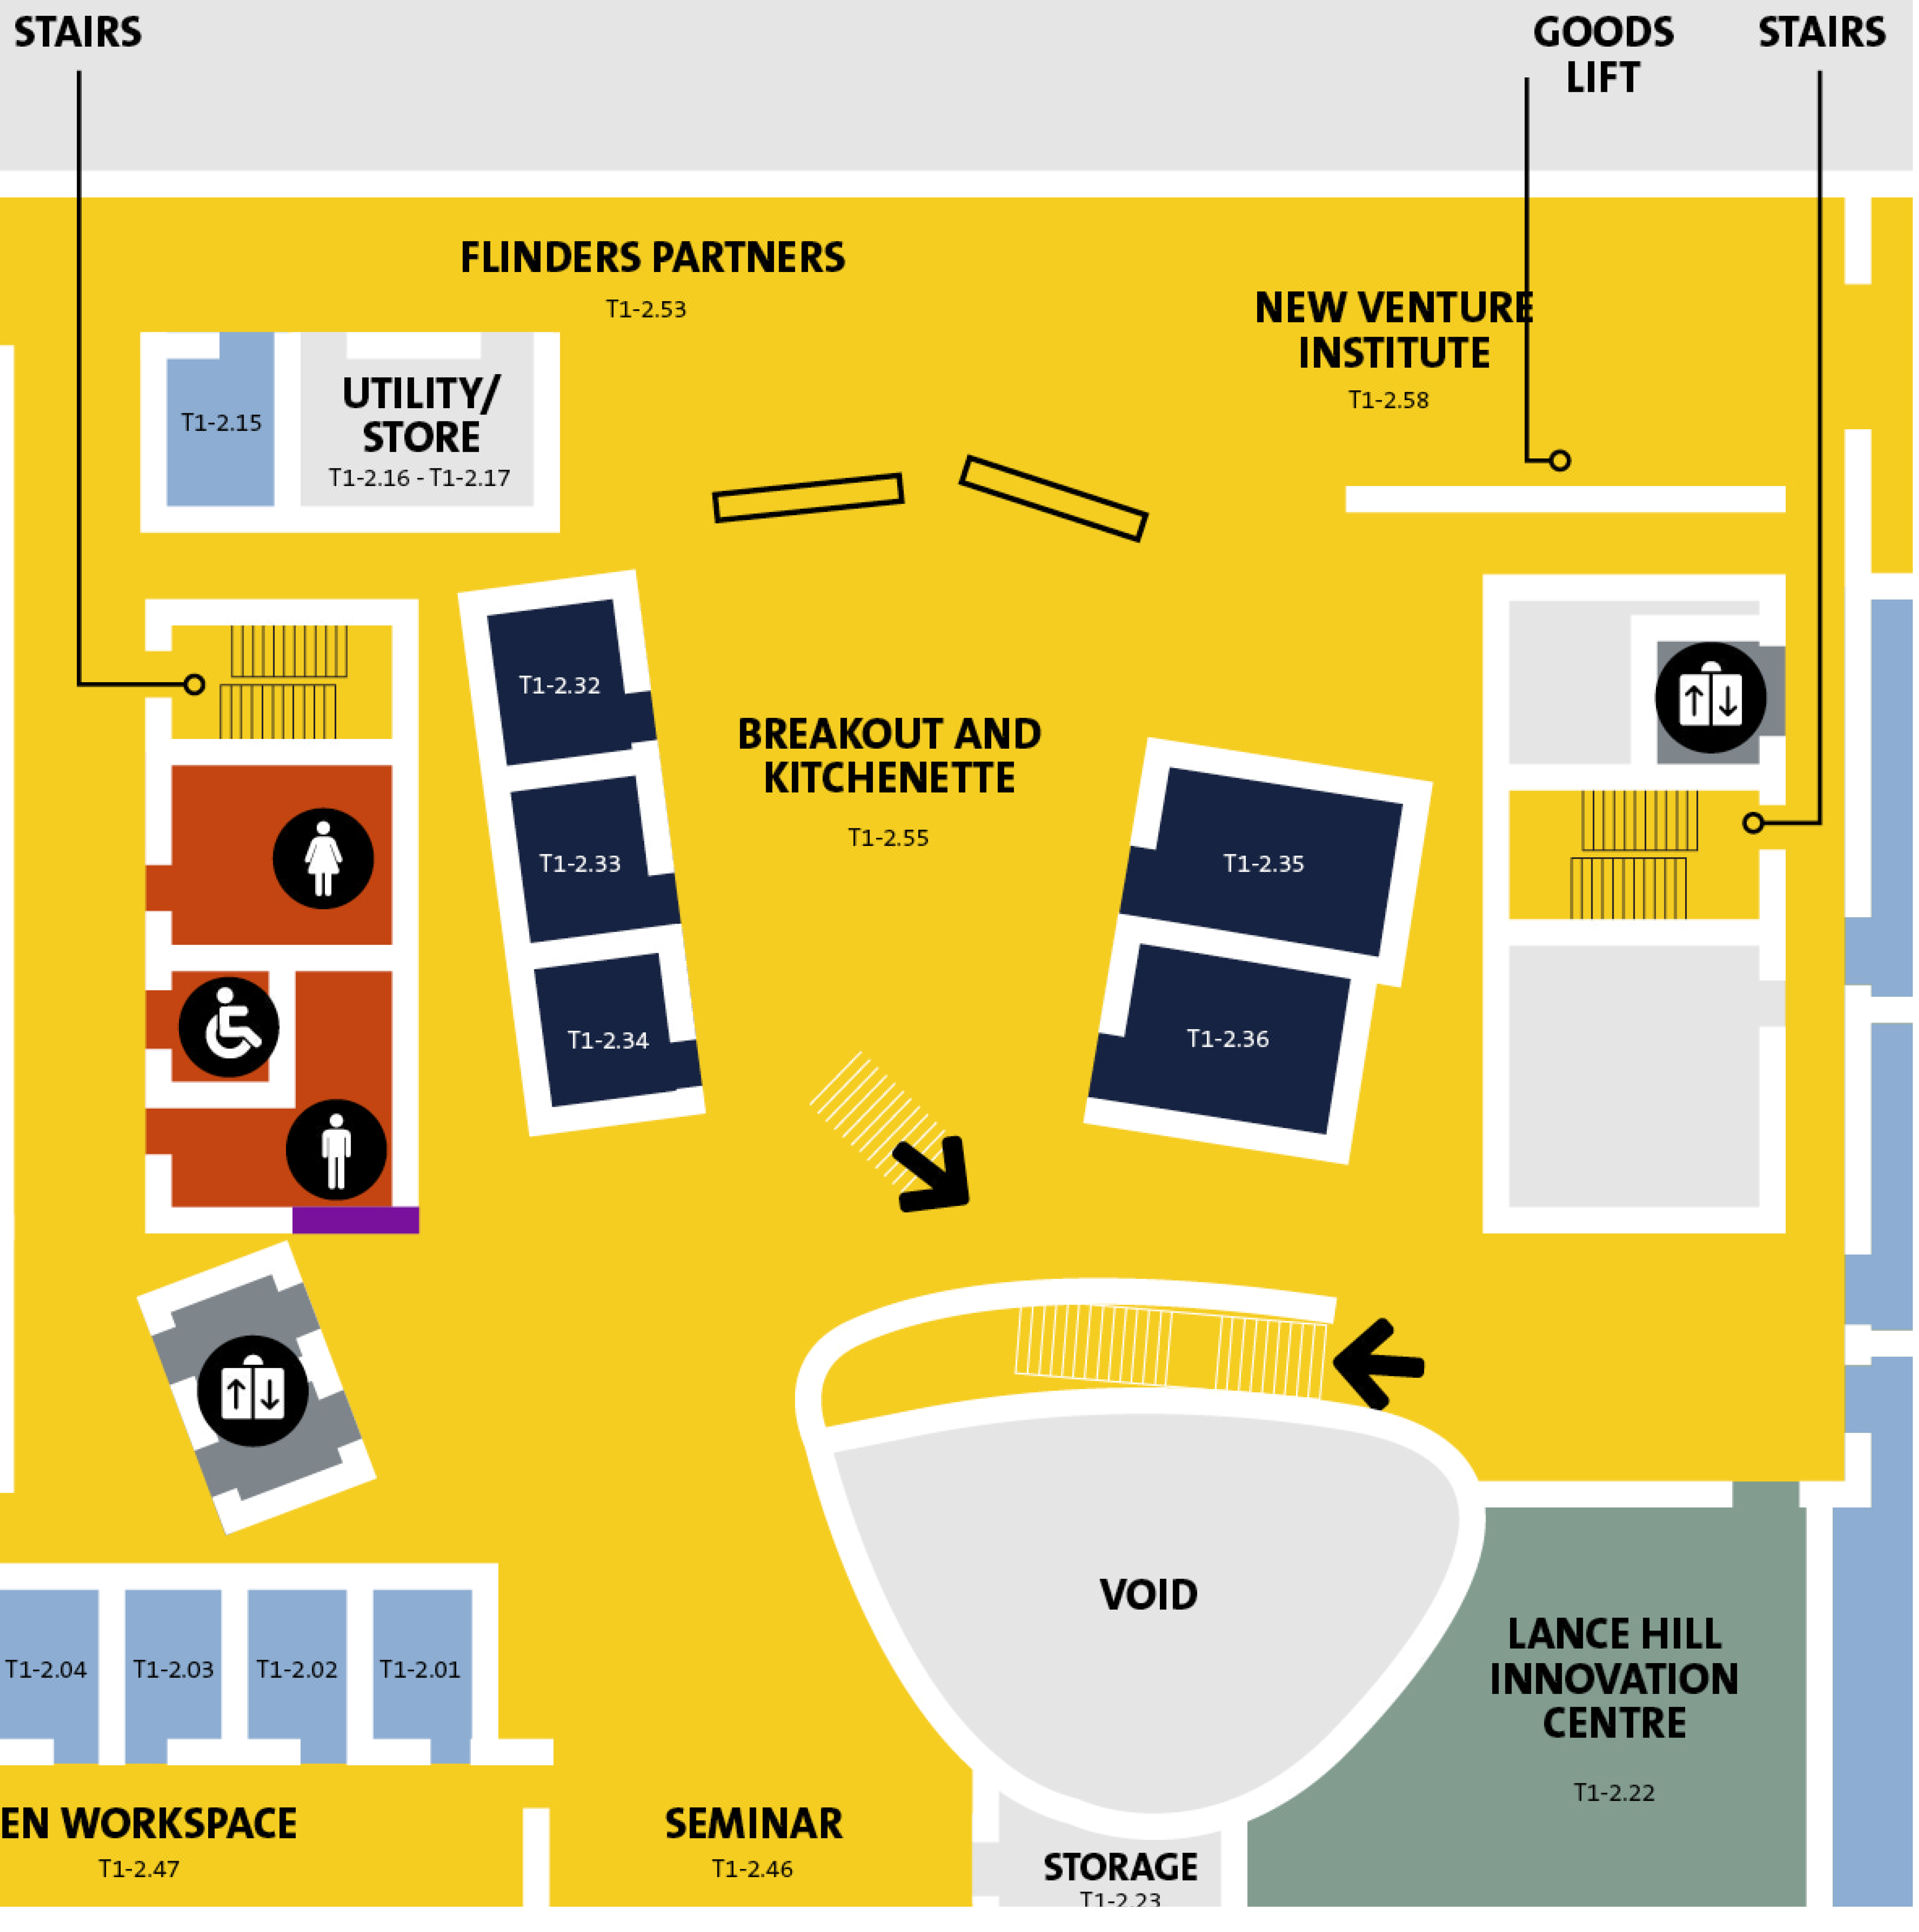
\includegraphics[width=0.3\textwidth]{image/T2.png}}}\hfill
\subfloat[Level 3]{\label{fig:btleft}{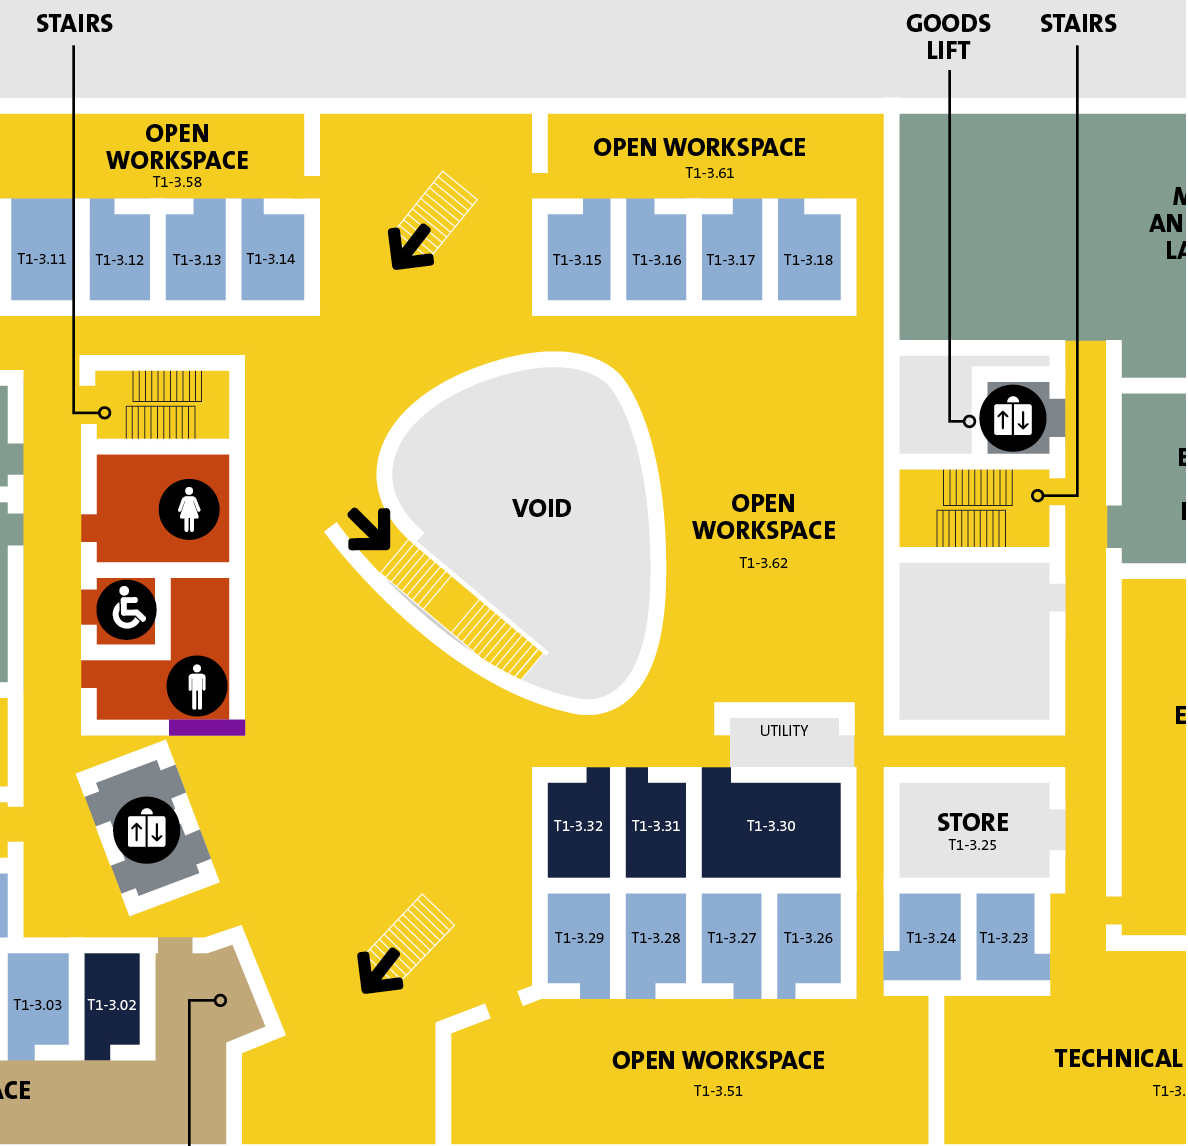
\includegraphics[width=0.3\textwidth]{image/T3.png}}}\hfill
\subfloat[Level 4]{\label{fig:md1}{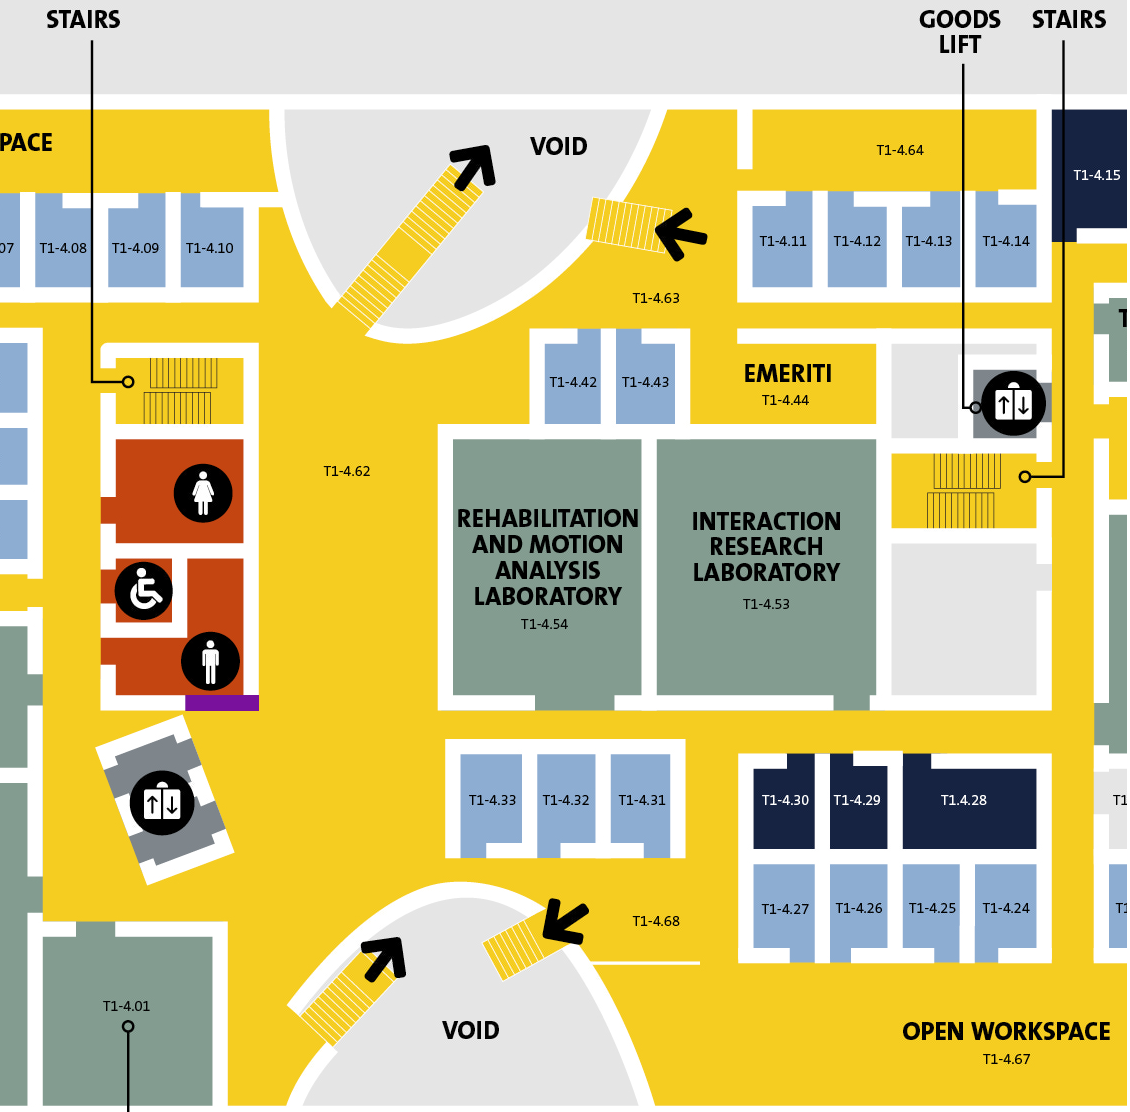
\includegraphics[width=0.3\textwidth]{image/T4.png}}}\hfill
\subfloat[Level 5]{\label{fig:mdright1}{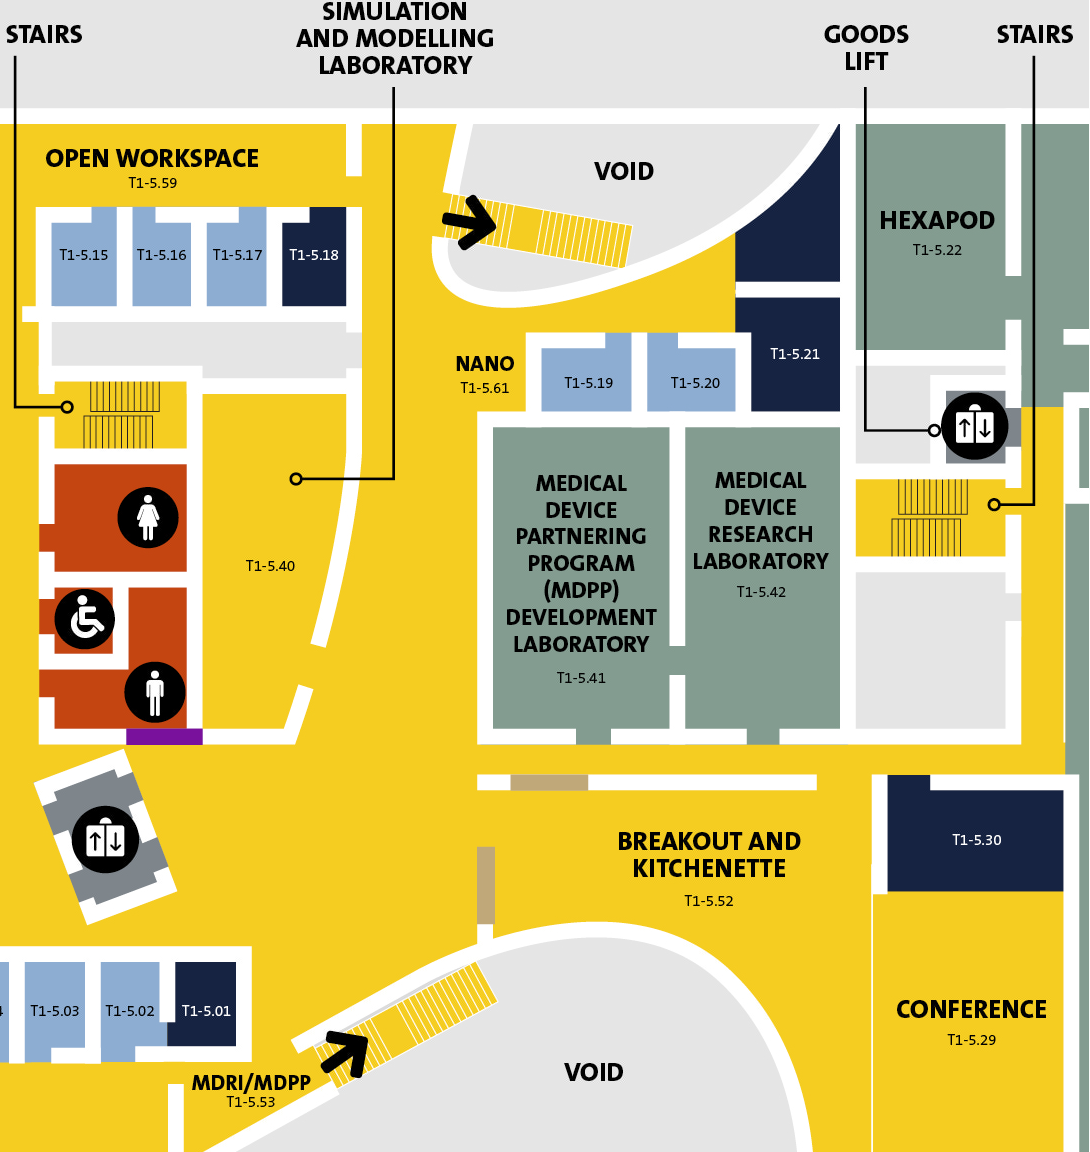
\includegraphics[width=0.3\textwidth]{image/T5.png}}}
\caption{Tonsley Building Layout. (a) Tonsley building view from the north-side parking lot, (b)-(f) Layout of levels 1-5.}
\label{laay}
\end{figure*}

E-counter sensors were deployed at all stairs. They are made by the International Road Dynamics company and consist of a pair of transmitter and receiver(transmitter: PTx20-1 and receiver: PRx20W1). The transmitter sends an infrared message to the receiver, when the infrared light is interrupted by someone passing through it, a count is registered. If no one passes, then these sensors log a count value of zero every 10 minutes. Each stair has two sensors, UP/DOWN that determine a person's direction of travel up and down the stairs. Signals from the sensors are sent to wireless hubs in real-time and then from the hubs to the server. The specification of all the sensors from this company are shown in Table \ref{sensor}. The maximum count value for each direction is about 1,000,000.

\begin{table}[!h]{}
 \small
\centering
\caption{E-counter sensors of International Road Dynamics company}%\cite{people}.}
\begin{tabular}{llll}
 \toprule
\textbf{Features} & \textbf{Transmitter} & \textbf{Receiver}  & \textbf{Applications}     \\
\midrule
 Display/Wireless/Bidirectional     &  PTx20-1 & PRx20WD1 & Entrance and daily counts\\ 
Wireless/Bidirectional             &  PTx20-1 & PRx20W1  & Entrance and daily counts\\ 
 Display/Bidirectional              &  PTx20-1 & PRx20D1  & Entrance and daily counts\\ 
 USB/Bidirectional                  &  PTx20-1 & PRx20U2  & Entrance and daily counts\\ 
 Display/USB/Bidirectional          &  PTx20-1 & PRx20UD2 & Entrance and daily counts\\ 
 \bottomrule
 \label{sensor}
 \end{tabular}
 \end{table}



Each level has two types of location: level entrance and stairs. These entrances have two types of sensors: OUT/IN and two types of sensors for stairs as UP/DOWN. These are coded for all levels except level0-1, which is both a stair and an entrance, so it has the label UP/IN and DOWN/OUT, instead of either UP or DOWN (stairs) or IN or OUT (entrances).

%Data collection is the process of gathering and measuring information. The data collection method consists of two categories, quantitative and qualitative.Experimental research is a quantitative method. Interviews are qualitative methods.Surveys, observations, archival research and secondary data collection can be quantitative or qualitative methods.Hence, collecting streaming data needs time and facilities, we used two ready to use dataset and apply a stream simulation phase to use as data stream for our model.

%\subsection{E-counters Geographical Location}
%\subsubsection{People Counting Localization Indoor Dataset}

The data was collected from February 21, 2019, until July 16, 2019, but only three months of this data set was monitored for the experiment. The experiment was conducted for a period of three months from March 18 to June 23, 2019, as shown in Table \ref{tons}. During the first month period starting on March 18, 2019, data was collected to establish a baseline for staircase usage by making measurements as unobtrusively as possible. The mid-semester break from April 15-28 was excluded from the study. 

Motivational and educational interventions were made during the next month period starting from April 29, 2019 to increase stair usage. The interventions included digital screens that displayed health information and provided live feedback throughout the building, especially near the lifts. An additional month period starting on May 27, 2019 was observed in order to assess any long term changes in the stair use pattern after the end of the intervention period. To keep the stair usage experiment duration separate from the rest of the data, it is saved in a different .CSV file to be used for pre-processing. 
%which provides us with a valuable 3-month dataset to model stair usage in a campus environment.


\begin{table}[ht]
\setlength{\arrayrulewidth}{0.5mm}
\setlength{\tabcolsep}{18pt}
    \centering
    \caption{Experiment timeline at Tensely Building for three months of intervention. The green color shows the before intervention month, the blue color indicates the intervention month, and the yellow color represents the month after the intervention period. The red and pink colors represented anomalous periods and are out of scope for this experiment.}
    \label{tons}
    \begin{tabular}{c c c}
    \hline
     \textbf{Semester Weeks} & \textbf{Timeline} & \textbf{Date} \\
     \hline\midrule
    \rowcolor{green}
     week 12 &  Baseline(Before intervention)  &  3/18/2019 \\
     \hline
    \rowcolor{green}
     week 13 & Baseline  & 3/25/2019 \\
     \hline
    \rowcolor{green}
     week 14 & Baseline   & 4/1/2019 \\
     \hline
    \rowcolor{green}
    week 15 &   Baseline & 4/8/2019 \\
     \hline
     \rowcolor{pink}
        & Mid Semester Break  & 4/15/2019 \\
      \hline
     \rowcolor{pink}
      &  Mid Semester Break  & 4/22/2019 \\
     \hline
     \rowcolor{cyan}
     week 18 & Intervention  & 4/29/2019 \\
     \hline
     \rowcolor{cyan}
     week 19 & Intervention   & 5/6/2019 \\
     \hline
     \rowcolor{cyan}
    week 20 &   Intervention & 5/13/2019 \\
     \hline
     \rowcolor{cyan}
      week 21  & Intervention  &  5/20/2019 \\
      \hline
     \rowcolor{yellow}
     week 22 &  Follow-up(After Intervention)  & 5/27/2019 \\
     \hline
     \rowcolor{yellow}
     week 23 & Follow-up  & 6/3/2019 \\
     \hline
     \rowcolor{yellow}
     week 24 & Follow-up   & 6/10/2019 \\
     \hline
     \rowcolor{yellow}
    week 25 &   Follow-up & 6/17/2019 \\
     \hline
     \rowcolor{red}
        & Exams  & 6/24/2019 \\
      \hline
     \rowcolor{red}
        & Exams  & 7/1/2019 \\
      \hline
      \rowcolor{pink}
         & Semester Break  &  7/8/2019 \\
      \hline
      \rowcolor{pink}
         & Semester Break  & 7/15/2019 \\
      \hline
      \rowcolor{pink}
         & Semester Break  &  7/22/2019 \\
      \hline
      
    \end{tabular}
    
\end{table}



The sensors captured movement for all 24 hours and all days continuously. The raw e-counter data set consists of approximately 668,000 data points, each containing nine attributes as listed in Table \ref{attr} out of which almost half the data points were included in our research work. 


\begin{table}[!h]{}
\centering
\caption{List of attributes for the e-counter data set}

    \begin{tabular}{p{2cm} p{3.5cm}  p{4.5cm} }
    \hline
    \textbf{Attribute} & \textbf{Measurement} & \textbf{Definition}\\ \hline
    \midrule
Date             &  mm/dd/yyyy      &   Date of measurement                                 \\\hline
Time             &  hh:mm:ss 24H    &   Time of measurement                                 \\\hline
Count            &  integer         &   Number of people counted by the sensor              \\ \hline
Sensor           &  Up, Down, In, Out, IN/Out-reserved & Direction of the sensor             \\ \hline
Position         &    string         &   Sensor location in the building                                                                                                      \\ \hline
Location Code    &     H2-L3             & Code for each location                                                                                                                                       \\ \hline
    \bottomrule
    \label{attr}
\end{tabular}
\end{table}





%The total number of people using the stairs over the entire experiment duration is shown in figure 2. It is apparent that people prefer taking the stairs to go down. An expected periodic lower occupancy is also observed on the weekends. The mid-semester break from April 15-28 was excluded from the study.


%\item\textbf{Data Pre-processing:}
During pre-processing, some issues were detected during the experiment period that affected the quality of our model. For instance, hubs were temporarily switched off or sensors fell off. Also, some special events took place during the experiment, such as public holidays, term breaks, and fire drills which affected the number of people using the stairs. For example, on May 1$^{st}$ at 11:15 a.m, the fire alarm went on, and everyone had to evacuate the building using the stairs. Also, between baseline duration and initiation of intervention, there was a two-week Easter break or semester break and that is why the intervention started after two weeks of the first stage. The data collected during the interrupted days mentioned above have not been included in the cluster analysis.

Furthermore, if no one passes through the beam of sensors, the sensors indicate zero during that specific interval. A huge number of zeros were logged during the experiment especially after working hours, weekends, and holidays, which could bias the clustering results. These zero values were removed from the data set. 

The e-counters save the position values as a string character combination of numbers and strings. Hence, it was also necessary to convert the string format of the position values into the integer format in order to allow us to use them as an input for the DSAP algorithm. 
%or fire alarm went to alarm for evacuation. This leads to having missing data points during data stream.%In addition, on May 7, printer level 5 broken and people had to use the stairs to get printer level 4.
Finally, the feature selection task was performed to provide a target data set ready to be used by the simulation and clustering. The Position and Count features were selected for computing the clusters. The hyperparameters for the AP in the DSAP algorithm are consistent and fixed for the entire experiment. The damping value is equal to 0.96, maximum iteration is 100, and preference is equal to the median of the similarity matrix.



% \begin{table}[!h]{}
% \centering
% \caption{Selected input variables for clustering the e-counter dataset.}

%     \begin{tabular}{p{3cm} l p{3cm} l  p{3cm} }
%     \hline
%     \textbf{Attribute} & \textbf{Description} & \textbf{Values} \\ \hline
%     \midrule
%      Position             &   The location of sensors installed in this building     
%      & Level2-1, Level3-2Central, Level4-3North, Level4-3South, Level5-4North, Level5-4South \\ \hline
%      Count               &  Number of people pass through the sensors    &   Integer:1,...n \\
%     \hline
%     \bottomrule
%     \label{variab}
% \end{tabular}
% \end{table}



%\item\textbf{Data Stream Simulation:}
%In order to mimic the data coming from an infinite stream, it was necessary to convert the limited duration into a data stream. The data stream simulation tools that are used are Scikit-Multiflow in Python and DSD in R. The reason why we have chosen these two simulations is that the DSAP algorithm has developed in Python, and the streaming K-means is implemented in the R programming language. 
%The target input dataset used for gathering the stream simulation is demonstrates in Table \ref{datain}. 

%To implement data stream for the DSAP algorithm with Scikit-Multiflow, we applied \textit{skmultiflow.data.FileStream} class for generating data stream out of our e-counter CSV file. The input of this class is a window with the size of l data point. Streaming K-means simulates data stream with Data Stream Data (DSD) object is used the package \textit{'stream'} by applying the \textit{DSD\_ReadCSV} function, which is a connector to the real-world data. The input of this function is the e-counter CSV file, and the output is a list of data points which the window updates every time frame by applying \textit{Update} function.

% \begin{table*}[ht]
% \centering
% \caption{the input data for the stream simulation.}
% \begin{tabular}{clclclc}
% \toprule
% \textbf{Date} & \textbf{Time} & \textbf{Position} &\textbf{Count}     \\
% \midrule
% 3/18/2019             & 8:12:31      &      4    &      1       \\
% 3/18/2019             & 8:32:31      &      4    &      2       \\
% 3/18/2019             & 8:52:31      &      4    &      1       \\
% ...                   &  ...         &      ...  &      ...     \\
% ...                   &  ...         &      ...  &      ...     \\
% 6/23/2019             & 19:13:01     &      6    &      1       \\
% 6/23/2019             & 19:23:01     &      3    &      1       \\
% \bottomrule
% \label{datain}
% \end{tabular}
% \end{table*}

%main itemize

%\end{itemize}


%%%%%%%%%%%%%%%%%%%%%%%%%%%%%
% I think we can remove this subsection. I can explain in next chapter
% \subsubsection{Data Stream Clustering}
% The measurements from the e-counters were analyzed to find patterns in time and space. Clusters of similar measurements with respect to position and count were generated using the DSAP and streaming K-means algorithms. To initiate the clustering algorithms, the size of the landmark time window needs to be defined. Different windows sizes ranging from 1 hour to 30 hours were test with the DSAP algorithm. A reasonable compromise between speed and accuracy of clusters was obtained for a window size of 5 hours, hence this was chosen as the size of the landmark window.% and because the number of people using the stairs are usually not significant or after working hours there is not much commuting, we consider each window with the length of 4 hour.
% There are several hyper parameters that need to be set in order to use the DSAP and streaming K-means algorithms correctly. This values are a function of the dataset under study. 
% \begin{itemize}
%     \item The damping factor for AP algorithm is constant for all AP function called and is equal to 0.9
%     \item The maximum iteration is the predefined value and it is 100.
%     \item The preference hyperparameter is the median value of the similarity matrix.
%     \item The expiration value equal to forget older windows is the last 5 landmark window (If it was applied). 
%     \item The landmark time frame is equal to every 5 hours.
% %    \item For the streaming k means algorithm the number of the macro clusters was obtained by the elbow method. This number is $k$ = 6 for the entire dataset.
% \end{itemize}












%  The same landmark window was used in the online clustering phase to generate micro-clusters. Once the data stream ended and all the micro clusters have been stored, the DSC function generation was again used for the computation of the macro clusters in the offline macro clustering Phase. 


%The data frame used for this dataset is every 4 hours. 

% \begin{itemize}
%     \item Preference parameter: the median value of the similarity matrix.
%     \item Damping factor: is equal to best result and reach convergence.
%     \item Maximum number of iteration and Convergence iteration: default values.
%     \item Threshold (comparing each new data point with the model): the minimum distance of data points to the centroids.

% \end{itemize}
   
% The online clustering initialises with 200 data points where gradually over time new data points are introduced and old data points are disposed. Micro-clusters were generated in each of these windows using the DSC function generation, and stored once the sliding window passed over the 200th data point relative to the starting data point.

% With a fixed number of cluster k = 4, for each landmark time window based on elbow method have been done separately, and once the data stream is ended and the micro clusters stored, the DSC function generation was again used for the computation of the macro clusters in the offline macro clustering Phase.

% In the end, to evaluate the performance of the clustering and compare two algorithm's clustering result for the e-counter dataset, different metrics are applied. Silhouette Coefficient, Calinski-Harabasz Index, and Davies-Bouldin Index, are calculated with two metrics obtain from clusters: cluster centroids and cluster labels. Processing time is calculated by subtract the end time from starting time with the  $time()$ method. Memory usage obtained from $psutil$ library in Python for processes and system utilization as same as $memory$ in R programming language. 

% We will go through these two stages below. 
    
%     \begin{itemize}
%         \item\textbf{DSC\_Window:} provides a clustering interface to the data stream operator $DSC\_Window$. It implements the sliding window model, which keeps a specified number of the most recent data points of the stream defines by the user. This number is the window length. 
        
%         \item\textbf{DSC\_Kmeans:} interface is the R version of K-means clustering implementation and a version of k-means where the data points (micro-clusters) are weighted by the micro cluster weights. The streaming k-means clustering algorithm requires continuously update the calculation of micro clusters.
        
%         For e-counter dataset, we used elbow method to find out the number of clusters which is equal to $k$ = 6. Also, same as the DSAP algorithm, the 10 minutes time frame was taken as a size of window. Once the data stream finished and the micro clusters collected all data points during this phase, the DSC function generation is used again to compute the macro clusters in the offline phase.
        
%     \end{itemize}
    

% \subsubsection{Clustering Performance Evaluation Phase}
% In order to compare the performance of the DSAP algorithm with streaming K-means clustering, the evaluation criteria discussed earlier in Section 4.4, were implemented using Python and R libraries. All the metrics implemented in Python are part of the $'Sklearn.metrics'$ library in Python and $'clusterCrit'$ in R including score functions and performance metrics. The input for Silhouette Coefficient, Calinski-Harabasz, and Davies-Bouldin Indexes are two parameter: centroids and label of clusters. The centroids are the output from streaming algorithms and the labels are predicted labels for each selected centroids. The output of each score is a floating number related to the clusters.

% The execution time of the clusters is another measurement to compare both DSAP and streaming K-means together. For the DSAP we used \textit{time()} function and for streaming K-means \textit{system.time} was used.

% Memory profiler in Python module for monitoring memory consumption of a process as well as line-by-line analysis of memory consumption for Python programs is used to estimate the memory consumption. It is a pure Python module that depends on the 'psutil' module. It first decorates the function you would like to profile with @profile and then runs the script with a special script (in this case with specific arguments to the Python interpreter).


    % \item \textbf{Silhouette Coefficient:} 
    %     \begin{itemize}
    %  \item  DSAP:
    %       \item Streaming K-means:
    %  \end{itemize}
    
    %To compute this factor for both Python and R programming language, we used Silhouette function the code below:
    % \begin{equation}
    %     sklearn.metrics.silhouette\_score(X, labels, *, metric='euclidean', sample\_size=None, random\_state=None, **kwds)
    %  \end{equation} 


% \begin{figure}
% \centering
% 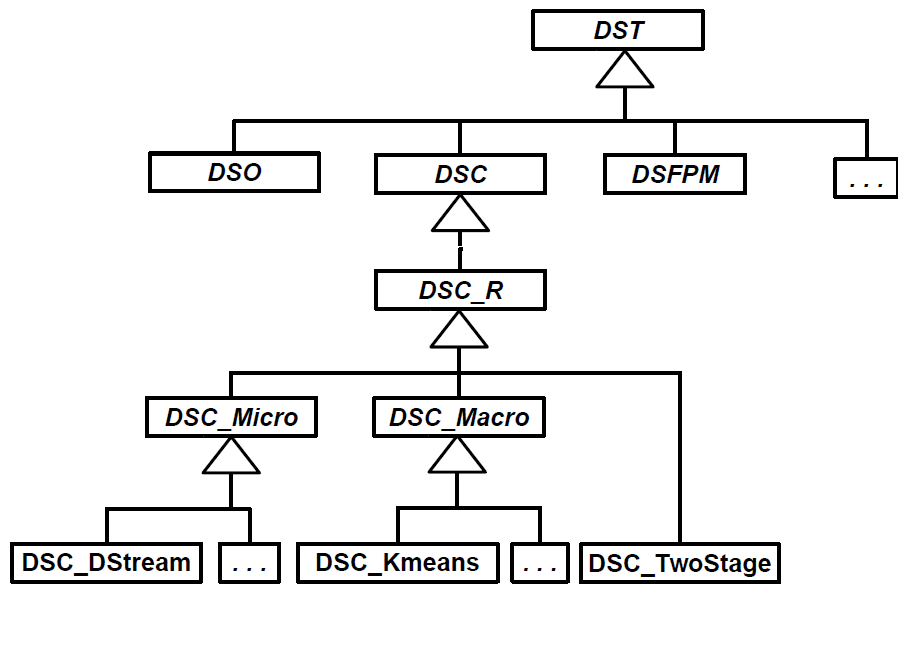
\includegraphics[width = 15cm,height = 9cm]{image/dst.png}
% \caption{Overview of data stream task (DST) \cite{hahsler2017introduction}. Overview of the data stream Data (DSD) class structure and data stream clustering (DSC) class structure with sub-classes.}
% \label{DSD}
% \end{figure}

%%%%%%%%%%%%%%%%%%%%%%%%%%%%%%%%%%%%%%%%%%%%%%%%%%%%%%%%%%%%%%%%%%%%%%%%%%%%%%%%%%%%%%%%%%%%%%%%

\section{Occupant Behaviour Experiment }\label{wifidat}

%The ubiquitous presence of wireless networks has brought opportunities for detecting non-intrusive human activity in an indoor environment. A significant advantage of the WAN fingerprint-based methods is that no additional hardware is needed as they use the existing WLAN infrastructure for position estimation. Therefore, the location of the user can be achieved without any expensive additional infrastructure. Accurate estimation of indoor location has applications in many areas including marketing, tracking products, assistance service in hospitals, etc. The WLAN Fingerprint-based Indoor Localization dataset, called UJIIndoorLoc dataset \cite{torres2014ujiindoorloc}, was one of the first publicly accessible and multi-storey database  to compare different indoor localization methodologies.  This experiment was conducted at the Universitat Jaume I (UJI), Spain, in 2013.

% \begin{figure}
%   \centering
% \sidesubfloat[]{\label{main:a}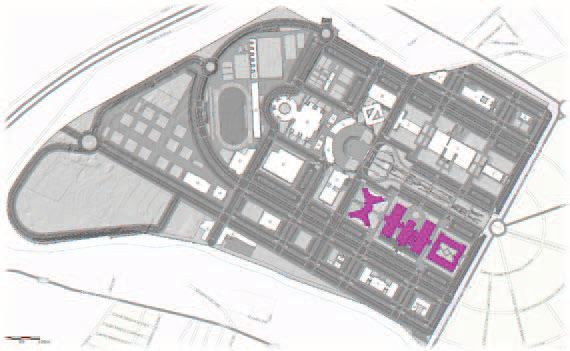
\includegraphics[width=0.4\linewidth]{image/uj1.png}}
%  \sidesubfloat[]{\label{main:b}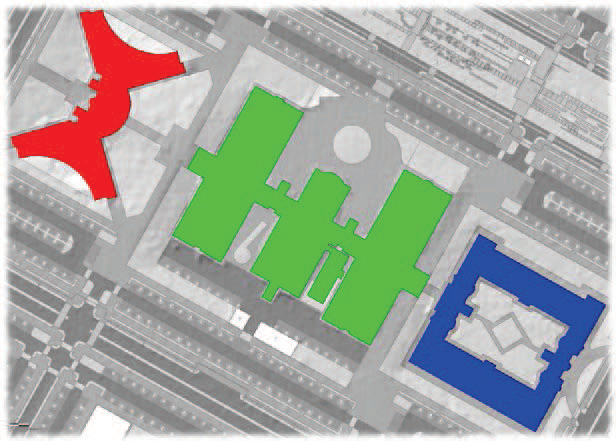
\includegraphics[width=0.4\linewidth]{image/uj2.png}}
% \bigskip
%     \caption{(a) Map of the UJI Riu Sec Campus and the buildings used for this experiment with purple color. (b) A zoom of these three buildings, T1 building show with the red color, TD building shows with the green color, and TC building shows with the blue color.}%\cite{torres2014ujiindoorloc}
%  \label{uji}
% \end{figure}


% \begin{figure*}[]%htb
% \begin{minipage}{.5\textwidth}
%   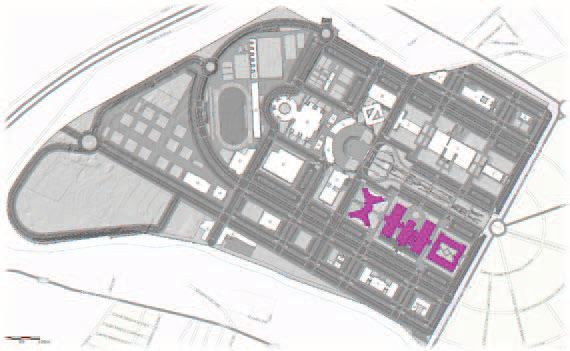
\includegraphics[width=1\textwidth]{image/uj1.png}
% \end{minipage}%
% \hfill
% \begin{minipage}{.5\textwidth}
%   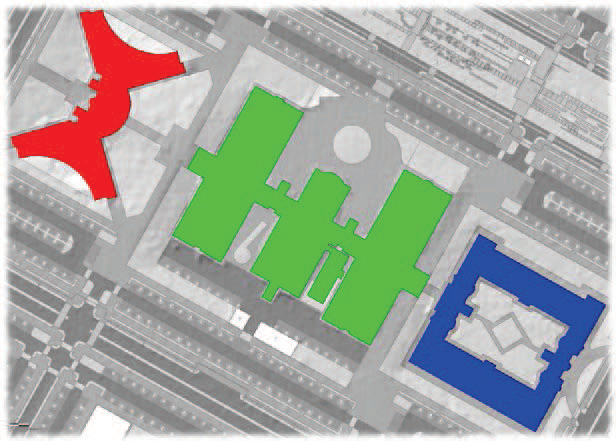
\includegraphics[width=.9\textwidth]{image/uj2.png}
% \end{minipage}
% \hfill
% \caption{(a) Map of the UJI Riu Sec Campus and the buildings used for this experiment with purple color. (b) A zoom of these three buildings, T1 building show with the red color, TD building shows with the green color, and TC building shows with the blue color.}
% \label{uji}
% \end{figure*}




%\subsubsection{Experiment}
% This experiment covers three buildings of Universitat Jaume I. It was created in 2013 by means of more than 20 different users and 25 Android devices.
% Samples were taken from random position

This case study was carried out to find occupant  behavior patterns  in  indoor  spaces  to provide  relevant  information  for  future planning  building  automation, evaluating energy efficiency scenarios, and simulating   emergency   protocols. The experiment was conducted over four months at the Universitat Jaume I campus, in Valencia, Spain. During this time, users carried mobile devices that used \textit{CaptureLoc} to record eight types of attributes including user position and WiFi signal strength across a total of thirteen levels spanning three buildings of the campus. To protect the identity of the participants during the course of the experiment, the unique MAC identifiers of the phones were hashed (anonymized) on reception.
%\begin{itemize}

%\item\textbf{Data Collection:}

% This experiment was conducted over four months at the UJI university campus and was divided in two sections: Training set and Validation set. 

The UJIIndoorLoc data set generated includes three buildings with four or more floors (one building has five floors) and almost 110.000 m$^{2}$of space. The total number of locations captured was 933. The shape and structure of the three buildings TI, TD, and TC, are quite different, as shown in Figure \ref{dspp2}. The raw data set consists of 19,938 data points containing 529 attributes as illustrated in Table \ref{featuj}. %These attributes include the Received signal strength indicator (RSSI) for 520 wireless access points (WAPs). The RSSI is an unitless number that provides an estimates of the  received signal strength.


\begin{figure*}[!h]
\centering
\subfloat[Overview of the three buildings]{\label{fig:build}{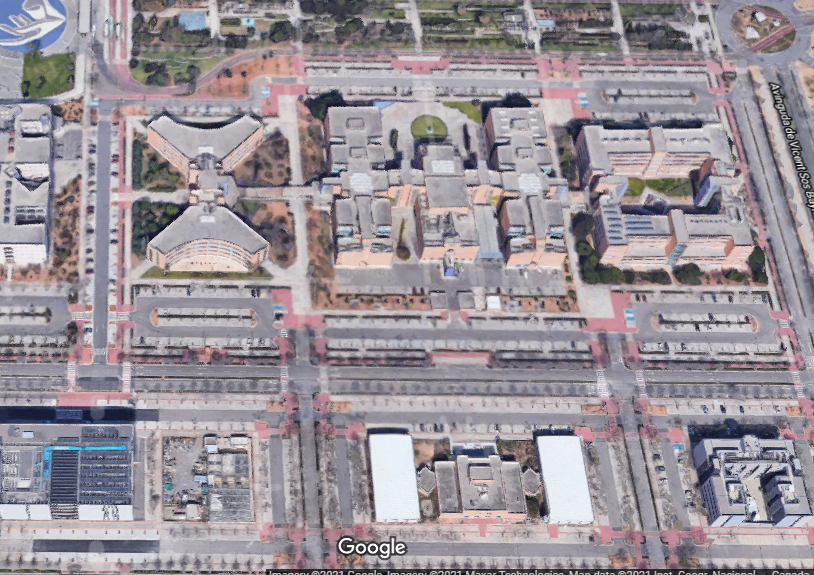
\includegraphics[width=7 cm, height = 6 cm]{image/Chapters/Chapter5/uji.PNG}}}\hfill
\subfloat[Building Number 0 (TI)]{\label{fig:bl2}{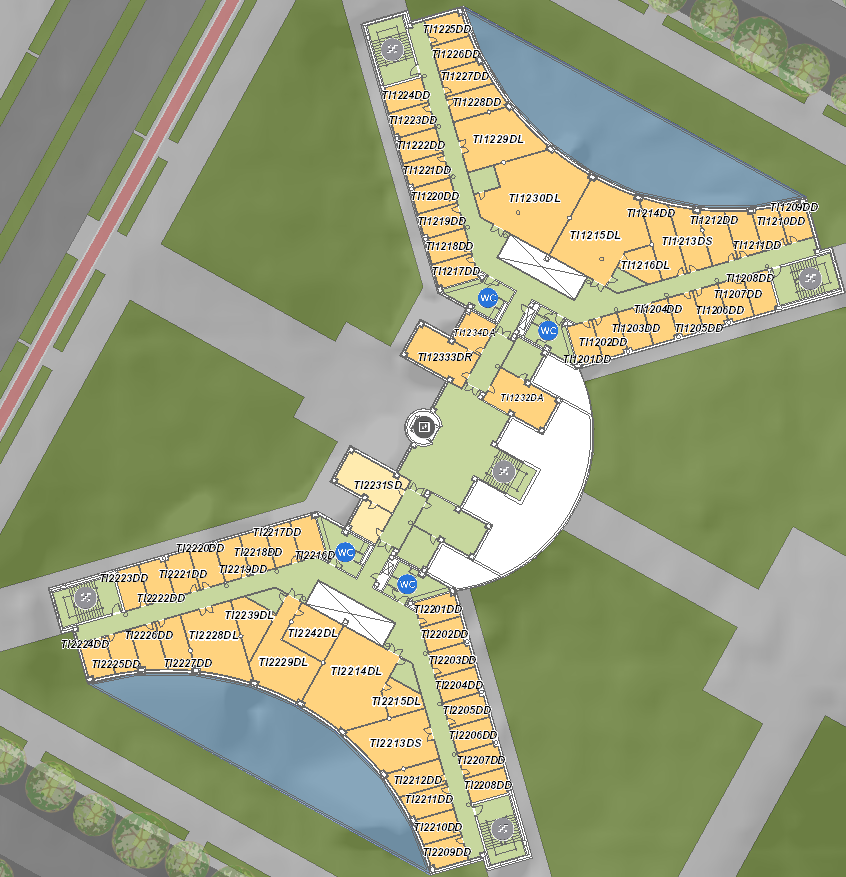
\includegraphics[width=0.4\textwidth]{image/plan2.png}}}\hfill
\subfloat[Building Number 1 (TD)]{\label{fig:bl3}{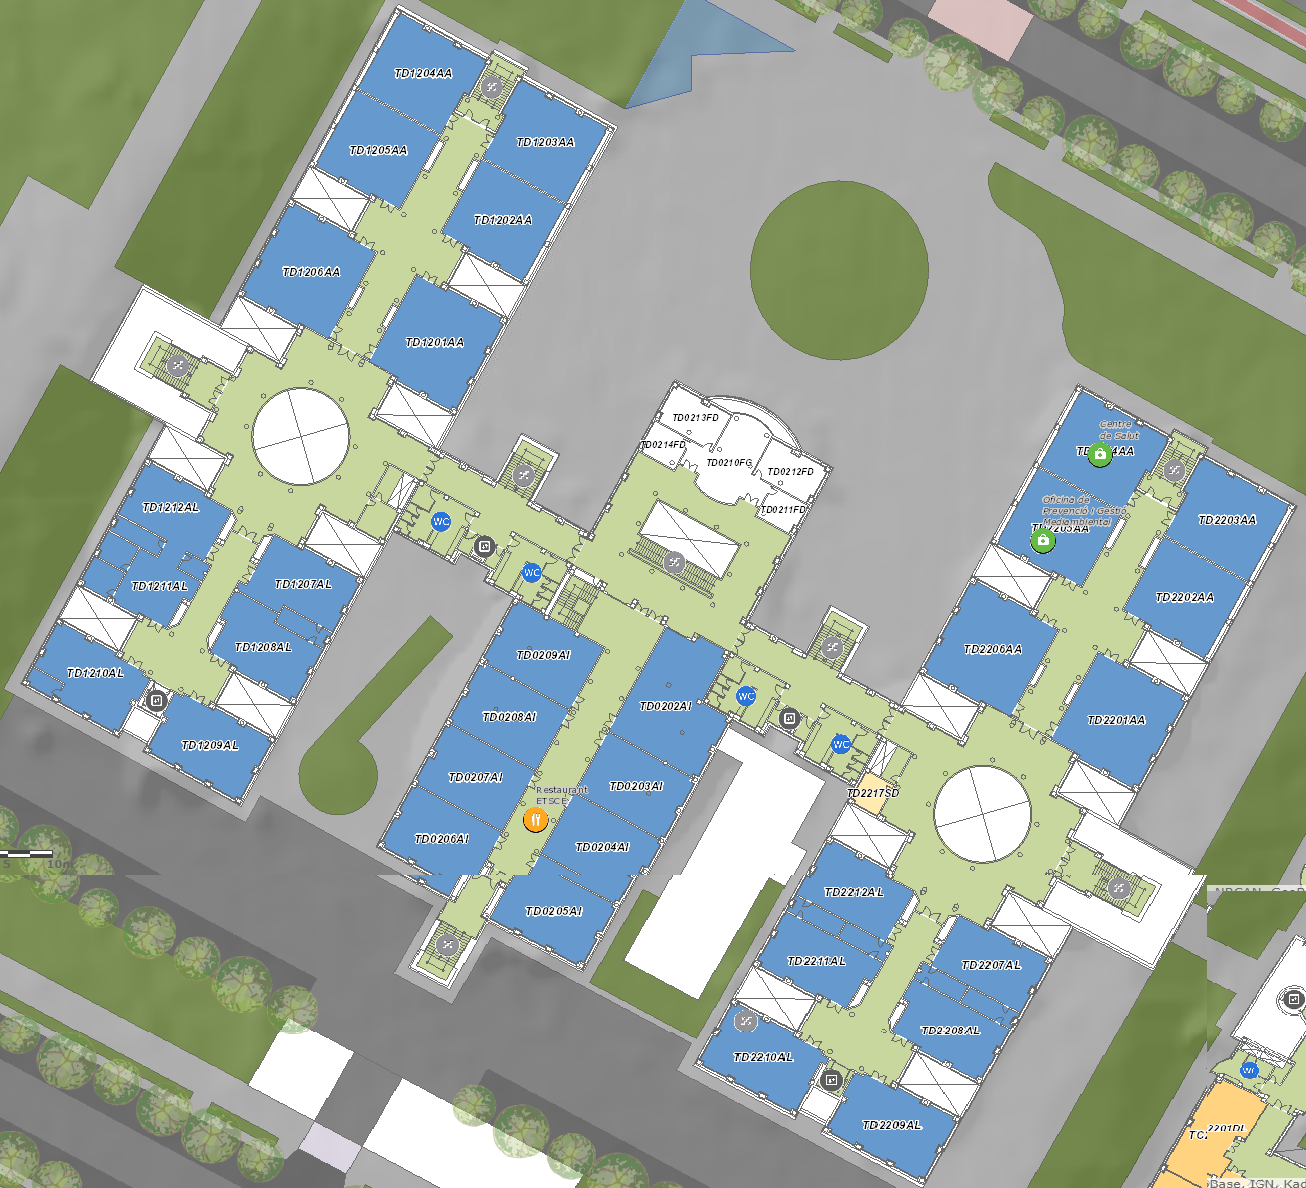
\includegraphics[width=0.4\textwidth]{image/plan3.png}}}\hfill
\subfloat[Building Number 2 (TC)]{\label{fig:bl4}{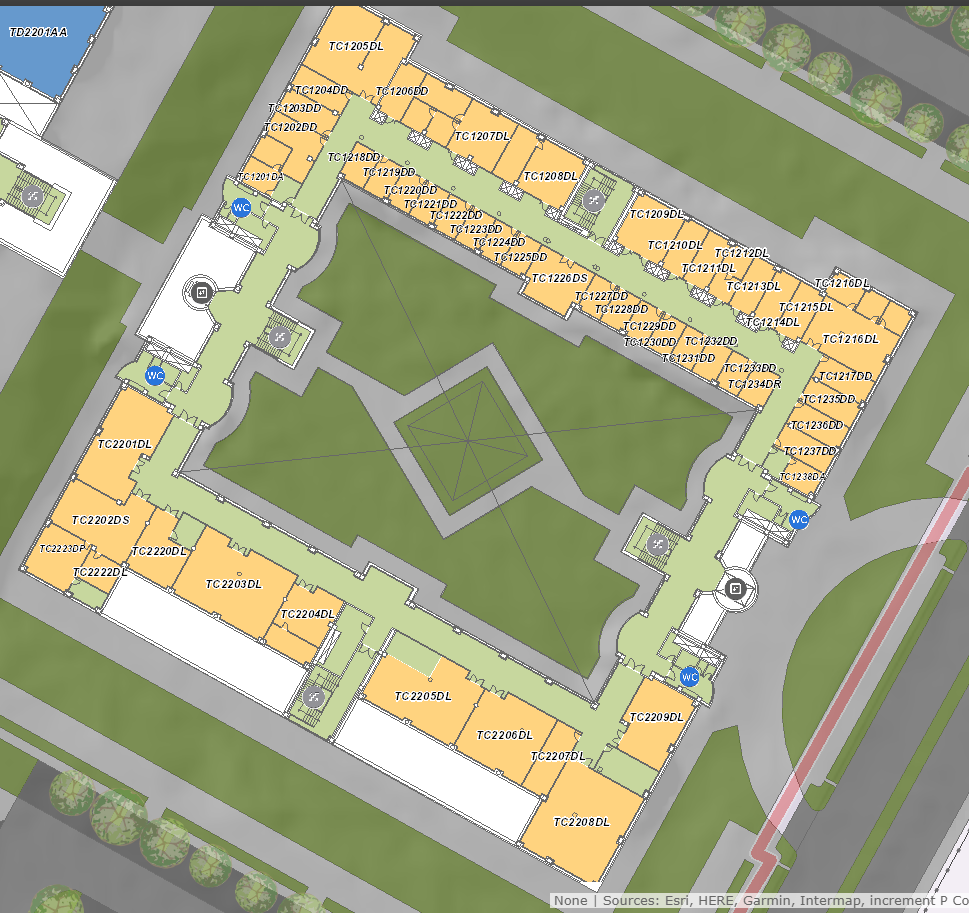
\includegraphics[width=0.4\textwidth]{image/plan1.png}}}\hfill
\caption{(a) Map of the UJI Riu Sec Campus and the buildings used for WiFi fingerprint experiment. (b,c,d) The layout of the three buildings with spaceid numbers for a floor.}% is shown with purple color. A zoom of T1, TD, and TC building shows. Inside the plans we have information regarding spaceID.}
\label{dspp2}
\end{figure*}

%***** remove 
\begin{table}[!h]{}
\centering
\caption{ List of attributes of the UJIIndoorLoc data set.}
\small
    \begin{tabular}{ p{4cm} p{4.5cm} p{4.5cm} }
    \hline
    \textbf{Attributes} & \textbf{Measurement} & \textbf{Definition} \\ \hline
    \midrule
    RSSI Level             &    -100dBM: weak signal, 0dBM: good, 100dBM: not detected    & RSSI levels where the WAP identifiers are linked to the vector positions           
    \\\hline
    Longitude              &    UTM from WGS84     &  Y coordinates           \\\hline
    Latitude               &    UTM from WGS84     &  X coordinates          \\\hline
    Floor                  &    0,1,2,3,4     &  Floors of each building           
    \\\hline
    Building ID            &    0,1,2     &  Each of the three buildings TI,TD, and TC          
    \\\hline
    Space ID               &    integer   & Identification of an indoor space (e.g. room or corridor)            
    \\\hline
    Relative Position      &    1= inside 2=outside       & Outside means in front of the door of the space \\\hline
    User ID                &    0,1,2,...,18    &  Unique code for users who participated in the experiment           \\\hline
    Phone ID               &    0,1,2,...,24      &    Android device code used for this experiment        \\\hline
    Timestamp              &    Unix time format      &  Time of capture           
    \\
    \bottomrule
\label{featuj}
\end{tabular}
\end{table}


% \\
% \textcolor{blue}{001-520: } RSSI levels\\
% \textcolor{blue}{521-524: } Real world coordinates of the sample points\\
% \textcolor{blue}{524: }\hspace{.75cm} BuildingID\\
% \textcolor{blue}{525: }\hspace{.75cm} SpaceID\\
% \textcolor{blue}{526: }\hspace{.75cm} Relative position with respect to SpaceID\\
% \textcolor{blue}{527: }\hspace{.75cm} UserID\\
% \textcolor{blue}{528: }\hspace{.75cm} PhoneID\\
% \textcolor{blue}{529: }\hspace{.75cm} Timestamp\\

% \begin{figure}[tbp]
%     \includegraphics[width=.3\textwidth]{image/uj1.png}\hfill
%     \includegraphics[width=.3\textwidth]{image/uj2.png}\hfill
%     \includegraphics[width=.3\textwidth]{image/uj3.png}
%     \\[\smallskipamount]
%     \caption{Map of the UJI Riu Sec Campus}
%     \label{uji}
% \end{figure}



% \begin{table}[!h]
%     \centering
%     \caption{ Sample information related to  PhoneID and real device. }
%     \label{phone}
%     \begin{tabular}{c c c c}
%     \hline
%      PhoneID & Android Device  & Android Version & UserID \\
%      \hline
%       0 &  Celkon A27  & 4.04 & 0\\
%      \hline
%       1 & GT-I8160   & 2.3.6 &8\\
%      \hline
%       2  &  GT-I8160 & 4.1.2 &0\\
%      \hline
%       3 & GT-I9100   & 4.0.4 &5\\
%      \hline
%       4  & GT-I9300  & 4.1.2 &0\\
%      \hline
%       5  & GT-I9505  & 4.2.2 & 0\\
%      \hline
%       6 & GT-S5360  &2.3.6  & 7\\
%      \hline
%       7 & GT-S6500  &2.3.6  &14\\
%      \hline
%       8 &  Galaxy Nexus  & 4.2.2  &10\\
%       \hline
%       9 &   Galaxy Nexus & 4.3 &0\\
%      \hline
%       10  & HTC Desire HD  &2.3.5 &0,11\\
%      \hline
%       11  & HTC One  & 4.1.2  & 0,1,9,16\\
%      \hline
%       12 &  HTC One & 4.2.2  & 3\\
%      \hline
%       13 &  HTC Wildfire S &2.3.5  &3\\
%      \hline
%       14 &  LT22i  & 4.0.4  &13\\
%       \hline
%       ... & ...   & ...  &...\\
%       \hline
%       24 & bq Curie   &  4.1.1 & 12\\
%       \hline
%     \end{tabular}
    
% \end{table}


The data was collected From May 30 to June 20, 2013 as shown in Table \ref{udate}. The number of data points show the distribution of measurements during each day. The data collection happened on these six discrete days. The day when the most amount of data was collected was the $20^{th}$ of June. This single day accounts for more than half the points in the entire data set.
%Two Android applications have been used to create the database by applying reference map services that are published in the ArcGIS. These services include geographic information inside the building. By using these services, the applications created show the maps to improve the user localization.


% all dataset capture in 6 days 30,31,may 4,10,12,20June, 19 , 20, 24,26 sep, 1,3,4,7,8 oct
\begin{table}[ht]
\centering
\caption{UJIIndoorLoc Experiment timeline.}
\begin{tabular}{lclc}
\toprule
\textbf{Date} &  \textbf{Number of data points}       \\
\midrule
     \rowcolor{cyan}
5/30/2019                 &      1140                 \\
     \rowcolor{cyan}
5/31/2019                 &      362                  \\
     \rowcolor{cyan}
6/4/2019                  &      1010                 \\
     \rowcolor{cyan}
6/10/2019                 &      270                 \\
     \rowcolor{cyan}
6/12/2019                 &      2467                 \\
     \rowcolor{cyan}
6/20/2019                 &      14688                \\
\bottomrule
\label{udate}
\end{tabular}
\end{table}



% \begin{enumerate}
%     \item\textbf{RSSI Levels:} These values show the RSSI levels by  WAP identifiers (MAC addresses) are linked to the vector positions. The RSSI levels represent negative integer values measured in dBm. In this measure, −100dBm is equivalent to the weak signal, and 0dBM indicates that the detected WAP is a very good signal. The value +100dBm in WAPs records shows that the signal has not been detected by the device.
%     \item\textbf{Real world coordinates:} It means three value, the longitude and latitude coordinates and the floor of the building. 
%     \item\textbf{Space identifier:} Is the value from 0 to 2 and corresponds the building campus. As figure \ref{uji} shows the UJI university campus
%     \item\textbf{User identifier:} This column ranges between 1 to 18 which 18 users are participated to gather the data. 
%     \item\textbf{Phone identifier:} It shows the android device used for this experiment. Table \ref{phone} shows the correspondence between each Phone ID and device used. The device's information included model and android version.
%     \item\textbf{Timestamp:} The time of when signal strength captured in Unix time format is available in the last column. This time is different with each phone time.
    
% \end{enumerate}



% \item\textbf{Data Pre-processing:}
A set of pre-processing tasks were performed to improve the quality of the data set and make the measurements suitable for cluster analysis.
%with the project scope and removed from the dataset.
The timestamp was recorded in a Linux-based time format, such as 1371714467, which corresponds to \texttt{06/20/2013 at 7:47 am}. All the time values were converted to the standard date-time format (dd/mm/yy hh:mm:ss) in Python and added as a new feature called Datetime into the data set.

The feature Space ID contains values starting from 1 to 250, but there were gaps between numbers 50-100 and 150-200. These gaps were removed, and the updated Space ID numbers range from 1 to 122.
These space ID values were not unique in terms of spaces such as offices, classrooms, and labs. 
The Space ID, Building ID, Floor, and relative position together provide a unique label for a location. A new feature is added to the data set called SPACEID, that contains a unique spatial identifier for each location. The SPACEID was created by combining the space identifiers and then giving them a sequential numbers from 0-732.

During the six days of collecting data, some phones (Phone ID = 0,2,4,5,9,12,15,20, and 21) were not used. To make it consecutive, gaps removed and a new feature called PHONEID added to the data with numbers between 1 to 16 for all presented phones.
Table \ref{phone} shows the phone ID related to each android device, the version of the operating system and finally, which user uses the phone. A total of 18 users with sixteen different phones are used for this research. The phone number 9 shared between three users with numbers 1, 9, and 16.




 

\begin{table}[!h]
    \centering
    \caption{ Correspondence between PhoneID, real device and userID. }
    \label{phone}
    \begin{tabular}{c c c c}
    \hline
     \textbf{PhoneID} & \textbf{Android Device}  & \textbf{Android Version} & \textbf{UserID} \\
     \hline\midrule
      1 & GT-I8160   & 2.3.6 &8\\
     \hline
      2 & GT-I9100   & 4.0.4 &5\\
     \hline
      3 & GT-S5360  &2.3.6  & 7\\
     \hline
      4 & GT-S6500  &2.3.6  &14\\
     \hline
      5 &  Galaxy Nexus  & 4.2.2  &10\\
      \hline
      6  & HTC Desire HD  &2.3.5 &18\\
     \hline
      7  & HTC One  & 4.1.2  & 15\\
     \hline
      8 &  HTC Wildfire S &2.3.5  &11 \\
     \hline
      9 &  LT22i  & 4.0.4  &1,9,16\\
     \hline
      10 &  LT26i  & 4.0.4  &3\\
      \hline      
      11 &  M1005D  & 4.0.4  &13\\
      \hline
      12 &  MT11i  & 2.3.4  &4\\
      \hline      
      13 &  Nexus 4 & 4.2.2  &6\\
      \hline     
      14 &  Orange Monte Carlo  & 2.3.5  &17\\
      \hline      
      15 &  Transformer TF101  & 4.0.3  &2\\
      \hline
      16 & bq Curie   &  4.1.1 & 12\\
      \hline\midrule
    \end{tabular}
    
\end{table}





% Two numerical variables were selected: the SPACEID and the Phone ID for this study as these provide the necessary information regarding the people present at any location with time. Finally, in order to remove bias due to the difference in range of the two variables the data was normalized. The normalization process is applied one level before clustering with the minmaxscaler normalization process under the preprocessing library. All these preceding steps provide a target data set ready to be used by the stream simulation and the two-phase clustering algorithms. 

For cluster analysis, The days are non-uniformly distributed over 2 month as shown in Table \ref{udate} earlier. The data collection during those six days was not continuous but collected at a much higher cadence. A small landmark time window of 10 minutes was applied on this dataset. Moreover, The hyperparameters for the AP in the DSAP algorithm are consistent and fixed for the entire experiment. The damping value is equal to 0.9, maximum iteration is 100, and preference is equal to the median of the similarity matrix. 

Finally, the variable selection task was performed to prepare a target data set ready to be used by the two phase clustering algorithm. For this research, two numerical variables as summarised in Table \ref{select2}.


\begin{table}[]
\centering
\caption{Selected input variables for clustering the data points}
\label{select2}
\begin{tabular}{
>{\columncolor[HTML]{FFFFFF}}c cc}
\hline
\textbf{Variable}              & \cellcolor[HTML]{FFFFFF}\textbf{Description}                                                          & \textbf{Values}     \\ \hline
{\color[HTML]{000000} PHONEID} & {\color[HTML]{000000} \begin{tabular}[c]{@{}c@{}}Each phone represents a\\  participant\end{tabular}} & Range between 1 -16 \\ \hline
{\color[HTML]{000000} SPACEID} & {\color[HTML]{000000} \begin{tabular}[c]{@{}c@{}}Each space represents a \\ location\end{tabular}}    & Range between 0-732 \\ \hline
\end{tabular}
\end{table}


% \begin{itemize}
%     \item A constant damping factor equal to 0.9 for AP algorithm.
%     \item The maximum iteration for AP is the predefined value and it is equal to 100.
%     \item The preference hyper-parameter for AP is the median value of the similarity matrix.
%     \item The expiration value equal to the last 5 landmark window is chosen. 
%     \item The time frame for this data is every 10 minutes.

    
% \end{itemize}


%\item\textbf{Data Stream Simulation:}
%In the simulation phase, we employed two techniques for our model as mentioned before for the for the e-counter data. These techniques are Scikit-Multiflow-based simulation for the DSAP algorithm in Python programming language and DSD-based simulation for the streaming K-means implements in R programming language. These methods are easy to use and can handle live stream from .CSV file. The input of this phase is UJIIndoorLoc dataset for generating the stream simulation and illustrated in Table\ref{ssiimm}. Scikit-Multiflow uses \textit{'skmultiflow.data.FileStream'} simulation class for batch dataset, and DSD used \textit{'stream'} package to implement the stream. 

% \begin{itemize}
%     \item \textbf{Scikit-Multiflow-based Simulations:}
%     \item \textbf{DSD-based Simulations:}
% \end{itemize}

% \begin{table}[!h]{}
% \centering
% \caption{The input data for stream simulation phase.}
% \begin{tabular}{lclcl}
% \toprule
% \textbf{Timestamp} & \textbf{SpaceID } & \textbf{PhoneID}    \\
% \midrule
% 5/30/2013 10:15:24             &   102    &     13       \\
% 5/30/2013 10:15:28             &   102    &     13       \\
% 5/30/2013 10:15:31             &   102    &     13       \\
% 5/30/2013 10:15:35             &   102    &     13       \\
% ...                            &   ...    &     ...      \\
% ...                            &   ...    &     ...      \\
% % 10/8/2013 3:56:47              &   0      &     13       \\
% % 10/8/2013 3:57:16              &   0      &     13       \\
% \bottomrule
% \label{ssiimm}
% \end{tabular}
% \end{table}


%\end{itemize}


% \subsubsection{Data Stream Clustering} 
% 




%Processing time is calculated by subtract the end time from starting time with the  $time()$ method. Memory usage obtained from $psutil$ library in Python for processes and system utilization as same as $memory$ in R programming language. Outlier Detection, Processing Time, and Memory Consumption. 

% \hspace{1 cm}

\section{System and Software}

Various tools and languages were used and they are listed below.

\begin{itemize}
    \item\textit{Platform:} This research work was performed on a personal computer running on a 64-bit operating system, window 10 Enterprise, 2019. The specification of this machine are: Intel Core i7 2.60GHz CPU, 32GB internal memory RAM, and 3TB external memory. 
    \item\textit{Language selection:} DSAP is developed in Python. The version of Python used is 3.7. Spyder 3.3.6 IDE which is part of Anaconda 2019 was used for project development. Main libraries applied in Python are sklearn, pandas, numpy, matplotlib, datetime, scipy, psutil and itertools.
    
    %Other programming language used for development and visualization are R and matlab. The versions used are RStudio 1.2.5033, 2019 and matlab 2019. 
    
    \item\textit{Software:} Microsoft Excel 2020 was used for preliminary visualization of the .CSV file format. It has a neat feature to quickly filter the data and visualize.
    
    Lucidchart web-based platform is another software that was used for drawing, revising and sharing charts and diagrams.
    

\end{itemize}

% some lat lang 2 user capture the poin t the same time with diffrent phones

% \end{document}


%%%%%%%%%%%%%%%%%%%%%%%%%%%%%%%%%%%%%%%%%%%%%%%%%%%%%%%%%%%%%%%%%%%%%%%%%%%%%%%%%%%%%%%%%%%%%%%%

% \section{Occupant Behaviour Experiment }\label{wifidat}


% This case study was carried out to find occupant  behavior patterns  in  indoor  spaces  to provide  relevant  information  for  future planning  building  automation, evaluating energy efficiency scenarios, and simulating   emergency   protocols. The experiment was conducted over four months at the Universitat Jaume I campus, in Valencia, Spain. During this time, users carried mobile devices that used \textit{CaptureLoc} to record eight types of attributes including user position and WiFi signal strength across a total of thirteen levels spanning three buildings of the campus. To protect the identity of the participants during the course of the experiment, the unique MAC identifiers of the phones were hashed (anonymized) on reception.


% The UJIIndoorLoc data set generated includes three buildings with four or more floors (one building has five floors) and almost 110.000 m$^{2}$of space. The total number of locations captured was 732. The shape and structure of the three buildings TI, TD, and TC, are quite different, as shown in Figure \ref{dspp2}. The raw data set consists of 19,937 data points containing 529 attributes as illustrated in Table \ref{featuj}. These attributes include the Received signal strength indicator (RSSI) for 520 wireless access points (WAPs). 

% \begin{figure*}[!h]
% \centering
% \subfloat[Overview of the three buildings]{\label{fig:build}{\includegraphics[width=7 cm, height = 6 cm]{image/Chapters/Chapter5/uji.PNG}}}\hfill
% \subfloat[Building Number 0 (TI)]{\label{fig:bl2}{\includegraphics[width=0.4\textwidth]{image/plan2.png}}}\hfill
% \subfloat[Building Number 1 (TD)]{\label{fig:bl3}{\includegraphics[width=0.4\textwidth]{image/plan3.png}}}\hfill
% \subfloat[Building Number 2 (TC)]{\label{fig:bl4}{\includegraphics[width=0.4\textwidth]{image/plan1.png}}}\hfill
% \caption{(a) Map of the UJI Riu Sec Campus and the buildings used for WiFi fingerprint experiment. (b,c,d) The layout of the three buildings with spaceid numbers for a floor.}% is shown with purple color. A zoom of T1, TD, and TC building shows. Inside the plans we have information regarding spaceID.}
% \label{dspp2}
% \end{figure*}

% %***** remove 
% \begin{table}[!h]{}
% \centering
% \caption{ List of attributes of the UJIIndoorLoc data set.}
% \small
%     \begin{tabular}{ p{4cm} p{4.5cm} p{4.5cm} }
%     \hline
%     \textbf{Attributes} & \textbf{Measurement} & \textbf{Definition} \\ \hline
%     \midrule
%     RSSI Level             &    -100dBM: weak signal, 0dBM: good, 100dBM: not detected    & RSSI levels where the WAP identifiers are linked to the vector positions           
%     \\\hline
%     Longitude              &    UTM from WGS84     &  Y coordinates           \\\hline
%     Latitude               &    UTM from WGS84     &  X coordinates          \\\hline
%     Floor                  &    0,1,2,3,4     &  Floors of each building           
%     \\\hline
%     Building ID            &    0,1,2     &  Each of the three buildings TI,TD, and TC          
%     \\\hline
%     Space ID               &    integer   & Identification of an indoor space (e.g. room or corridor)            
%     \\\hline
%     Relative Position      &    1= inside 2=outside       & Outside means in front of the door of the space \\\hline
%     User ID                &    1,2,...,18    &  Unique code for users who participated in the experiment           \\\hline
%     Phone ID               &    1,2,...,16      &    Android device code used for this experiment        \\\hline
%     Timestamp              &    Unix time format      &  Time of capture           
%     \\
%     \bottomrule
% \label{featuj}
% \end{tabular}
% \end{table}


% A total of 18 users with sixteen different phones participated in the study as listed in Table \ref{phone}. This table show the phone ID related to each android device, the version of the operating system and finally, which user uses the phone. The phone number 9 shared between three users with numbers 1, 9, and 16. 

% \begin{table}[!h]
%     \centering
%     \caption{ Sample information related to  PhoneID and real device. }
%     \label{phone}
%     \begin{tabular}{c c c c}
%     \hline
%      \textbf{PhoneID} & \textbf{Android Device}  & \textbf{Android Version} & \textbf{UserID} \\
%      \hline\midrule
%       1 & GT-I8160   & 2.3.6 &8\\
%      \hline
%       2 & GT-I9100   & 4.0.4 &5\\
%      \hline
%       3 & GT-S5360  &2.3.6  & 7\\
%      \hline
%       4 & GT-S6500  &2.3.6  &14\\
%      \hline
%       5 &  Galaxy Nexus  & 4.2.2  &10\\
%       \hline
%       6  & HTC Desire HD  &2.3.5 &18\\
%      \hline
%       7  & HTC One  & 4.1.2  & 15\\
%      \hline
%       8 &  HTC Wildfire S &2.3.5  &11 \\
%      \hline
%       9 &  LT22i  & 4.0.4  &1,9,16\\
%      \hline
%       10 &  LT26i  & 4.0.4  &3\\
%       \hline      
%       11 &  M1005D  & 4.0.4  &13\\
%       \hline
%       12 &  MT11i  & 2.3.4  &4\\
%       \hline      
%       13 &  Nexus 4 & 4.2.2  &6\\
%       \hline     
%       14 &  Orange Monte Carlo  & 2.3.5  &17\\
%       \hline      
%       15 &  Transformer TF101  & 4.0.3  &2\\
%       \hline
%       16 & bq Curie   &  4.1.1 & 12\\
%       \hline\midrule
%     \end{tabular}
    
% \end{table}


% % \begin{table}[!h]
% %     \centering
% %     \caption{ Sample information related to  PhoneID and real device. }
% %     \label{phone}
% %     \begin{tabular}{c c c c}
% %     \hline
% %      \textbf{PhoneID} & \textbf{Android Device}  & \textbf{Android Version} & \textbf{UserID} \\
% %      \hline\midrule
% %       1 & GT-I8160   & 2.3.6 &8\\
% %      \hline
% %       3 & GT-I9100   & 4.0.4 &5\\
% %      \hline
% %       6 & GT-S5360  &2.3.6  & 7\\
% %      \hline
% %       7 & GT-S6500  &2.3.6  &14\\
% %      \hline
% %       8 &  Galaxy Nexus  & 4.2.2  &10\\
% %       \hline
% %       10  & HTC Desire HD  &2.3.5 &18\\
% %      \hline
% %       11  & HTC One  & 4.1.2  & 15\\
% %      \hline
% %       13 &  HTC Wildfire S &2.3.5  &11 \\
% %      \hline
% %       15 &  LT22i  & 4.0.4  &1,9,16\\
% %      \hline
% %       16 &  LT26i  & 4.0.4  &3\\
% %       \hline      
% %      \hline
% %       17 &  M1005D  & 4.0.4  &13\\
% %       18 &  MT11i  & 2.3.4  &4\\
% %       \hline      
% %       19 &  Nexus 4 & 4.2.2  &6\\
% %       \hline     
% %       22 &  Orange Monte Carlo  & 2.3.5  &17\\
% %       \hline      
% %       23 &  Transformer TF101  & 4.0.3  &2\\
% %       \hline
% %       24 & bq Curie   &  4.1.1 & 12\\
% %       \hline\midrule
% %     \end{tabular}
    
% % \end{table}


% The data was collected From May to June 2013 as shown in Table \ref{udate}. The number of data points show the distribution of measurements during each day. The data collection happened on 6 discrete days. The day when the most amount of data was collected was the 20th of June. This single day accounts for more than half the points in the entire data set. 
% %Two Android applications have been used to create the database by applying reference map services that are published in the ArcGIS. These services include geographic information inside the building. By using these services, the applications created show the maps to improve the user localization.



% \begin{table}[ht]
% \centering
% \caption{UJIIndoorLoc Experiment timeline.}
% \begin{tabular}{lclc}
% \toprule
% \textbf{Date} &  \textbf{Number of data points}       \\
% \midrule
%      \rowcolor{cyan}
% 5/30/2019                 &      1140                 \\
%      \rowcolor{cyan}
% 5/31/2019                 &      362                  \\
%      \rowcolor{cyan}
% 6/4/2019                  &      1010                 \\
%      \rowcolor{cyan}
% 6/10/2019                 &      270                 \\
%      \rowcolor{cyan}
% 6/12/2019                 &      2467                 \\
%      \rowcolor{cyan}
% 6/20/2019                 &      14688                \\
%      \rowcolor{pink}
% 9/19/2019                 &      51                   \\
%      \rowcolor{pink}
% 9/20/2019                 &      133                  \\
%      \rowcolor{pink}
% 9/24/2019                  &     56                   \\
%      \rowcolor{pink}
% 9/26/2019                  &     69                   \\
%      \rowcolor{pink}
% 10/1/2019                  &     8                    \\
%      \rowcolor{pink}
% 10/3/2019                  &     8                    \\
%      \rowcolor{pink}
% 10/4/2019                  &     702                  \\
%      \rowcolor{pink}
% 10/7/2019                  &     81                   \\
%      \rowcolor{pink}
% 10/8/2019                  &     3                    \\
% \bottomrule
% \label{udate}
% \end{tabular}
% \end{table}



% A set of pre-processing tasks were performed to improve the quality of the data set and make the measurements suitable for cluster analysis.
% %with the project scope and removed from the dataset.
% The timestamp was recorded in a linux-based time format, such as 1371714467 which corresponds to 06/20/2013 at 7:47am. All the time values were converted to the standard date-time format (dd/mm/yy hh:mm:ss) in Python and added as a new feature called Datetime into the data set.

% The feature SpaceID contains values starting from 1 to 250, but there were gaps between numbers 50-100 and 150-200. These gaps were removed and the updated SpaceID numbers range from 1 to 122 now. During the validation part of the experiment a subset of the phones (PhoneID = 0,2,4,5,9,12,15,20, and 21) were not used. The remaining Phoneids were renamed to make the records sequential just like the SpaceIDs. The space identifiers, the SpaceID, BuildingID, Floor, and relative position together provide a unique label for a location. A new feature is added to the data set called SPACEID, that contains a unique spatial identifier for each location. The SPACEID was created by combining the space identifiers and then giving them a sequential numbers from 0-732.

% For cluster analysis, The days are non-uniformly distributed over 2 month as shown in Table \ref{udate} earlier. For the training data, The data collection during those six days was not continuous but collected at a much higher cadence. For these reasons a smaller landmark time window of 10 minutes was applied on this dataset. Moreover, The hyperparameters for the AP in the DSAP algorithm are consistent and fixed for the entire experiment. The damping value is equal to 0.9, maximum iteration is 100, and preference is equal to the median of the similarity matrix.
\include{Chapters/chapter6}
% \documentclass[../UNBThesis2.tex]{subfiles}
\setlength{\parindent}{2em}

% \begin{document}
\chapter{Conclusion and Future Work}

This research work was proposed a novel affinity propagation data stream clustering algorithm called DSAP with the implementation of the landmark time window model for keeping the updated data points from the stream. The DSAP model is capable of handling any form of streaming data. It is specially useful for extracting summery information from a large number of indoor localization and internet of things sensors which they have not been applied on AP stream clustering models.
The proposed DSAP algorithm was compared with the established streaming K-means algorithm and validate the clustering results based on the intrinsic clustering validation and performance evaluation metrics. These metrics which are 

Future research will explore other time window models such as sliding, damped and pyramidal models for the DSAP algorithm. Also, the event-based DSAP model is presented but we have not test it on these two datasets and next step will test our model with this format.

The next step for improvement DSAP is to having arcit


One specific feature of the presented work is to deal with application domains where a cluster of items cannot easily be represented by an average/artifact item, although the distance or similarity between any two items can be computed. I

other types of windows
detecting distribution
use real world data stream or benchmarking
try different distances 
swclustering
macro cluster user define
why not the current algo? we have k-means streaming but this is mean of data --> not useful for out data , we cant have mean of levels or people
macro --> end of stream but we need user request
indoor movement predict
algo --> if the number of micro cluster increase , weshould forget the old data
algo --> if the window end AP (but if there is no point?)
macro phase is not time sensetive. all micro clusters have same value(DCStream)
how is indoor positioning calculated
reoccurence detection(collect inactive clusters)
why ap? this algo works based on the distances. which is the best fit for our dataset. we havel levels and people. we cant use kmeansto give us a average distanfe which may be between 2 levels!
compare DSAP with other data srtream algorithm and diffrent dataset is future work
apply dsap with diffrent distances

DSAP still has some drawbacks such as handlind the old cluster and not through them out.
data distribution change by PH test or any other test
% \end{document}
good examples for stream clustering and clustering

% \subfile{Chapters/chapter1}
% \subfile{Chapters/chapter2}
% \subfile{Chapters/chapter3}
% \subfile{Chapters/chapter4}
% \subfile{Chapters/chapter5}
% \subfile{Chapters/chapter6}
% \subfile{Chapters/chapter7}
% %%----------------Bibliography--------------------------------
% \begin{thebibliography}{99}
% \addcontentsline{toc}{chapter}{Bibliography}
% \bibitem{k1} R.J. Drofnats, \emph{Proof of the Riemann
% Hypothesis},  preprint, available at
% \texttt{http://www.drofnats.com/riemann.ps}.

% \bibitem{k2} P. Erd\H os, \emph{A selection of problems and
% results in combinatorics}, Recent trends in combinatorics
% (Matrahaza, 1995), Cambridge Univ. Press, Cambridge, 2001, pp. 1--6.

% \bibitem{k3}
% R.L. Graham, D.E. Knuth, and O. Patashnik, \emph{Concrete
% mathematics}, Addison-Wesley, Reading, MA, 1989.

% \bibitem{Knuth92} D.E. Knuth, \emph{Two notes on notation}, Amer.
% Math. Monthly \textbf{99} (1992), 403--422.
% \bibitem{Drofnats} R.J. Drofnats, \emph{Proof of the Riemann
% Hypothesis},  preprint, available at
% \texttt{http://www.drofnats.com/riemann.ps}.

% \bibitem{Erdos01} P. Erd\H os, \emph{A selection of problems and
% results in combinatorics}, Recent trends in combinatorics
% (Matrahaza, 1995), Cambridge Univ. Press, Cambridge, 2001, pp. 1--6.


% \end{thebibliography}



% changes default name Bibliography to References
%\renewcommand{\bibname}{References}
\bibliographystyle{apacite}
% \bibliographystyle{amsplain}

\bibliography{mybibliography}
\addcontentsline{toc}{chapter}{Bibliography}
%%%---------------Appendices--------------------------------
\appendix
\chapter{this is Appendix A}
% In order to mimic the data coming from an infinite stream, it was necessary to convert the limited duration into a data stream. The data stream simulation tools are described next, followed by the description of the use cases.


% \section{Data Stream Simulation}
% Since data used in this research were obtained from concluded experiments, it was essential to find a mechanism to convert the batches of data in to a data stream. The streaming data was generated from the target datasets by applying the Scikit-Multiflow package in Python for the DSAP algorithm and the DSD objects in the stream package in R for the streaming K-means algorithm. 



% \subsection{Scikit-Multiflow-based Simulation}
% The 'scikit-multiflow' framework in Python programming language is a free and open-source tool for generating data stream \cite{montiel2018scikit}. It provides multiple stream learning methods, steam generators, and evaluators, where the primary focus is on batch learning. This framework's base class is the 'StreamModel', which has abstract methods to be implemented by classes. A 'StreamModel' object interacts with other objects: ' Stream' and 'StreamEvaluator'. The 'stream' gives an endless flow of data by request, and 'StreamEvaluator' presents various tasks that are queries the stream, train, test on the incoming data, and tracks the model's performance.

% 'scikit-multiflow' needs NumPy library installed in the system. All classes are shown in Figure \ref{sci} for generating data stream. The \textit{skmultiflow} data contains data stream methods, including methods for batch-to-stream conversion and generators. In all classes, the stream is available upon request and old data points cannot be accessed at a later time. These are listed below:

% %\renewcommand\labelitemi{$\vcenter{\hbox{\tiny$\bullet$}}$}
% \begin{itemize}
%     \item {data.base\_stream.Stream:} it defines the minimum requirements of a stream and it can work along with other modules in multiflow. 
%     \item {data.DataStream:} it takes the whole data consisting of the $X$ as features and $Y$ as targets or takes them separately.
%     \item {data.FileStream:} if the data previously collected and stored in the CSV file (it just supports CSV files at this moment), it can generate streams by loading the dataset. 
%     \item {data.ConceptDriftStream:} this stream generator adds concept drift by joining several streams and giving the weight. 
%     \item {data.TemporalDataStream:} takes the dataset containing $X$ as a features and $Y$ as a targets with $time$ as a timestamps. 
% \end{itemize}

% On the other hands, as shown in Figure \ref{sci}, there are many stream generators classes for different problems listed below:
% %\renewcommand\labelitemi{$\vcenter{\hbox{\tiny$\bullet$}}$}

% \begin{itemize}
%     \item[$-$]  data.WaveformGenerator: random differentiation of some base waveforms.
%     \item[$-$]  data.SineGenerator: sine waves stream generator.
%     \item[$-$]  data.AgrawalGenerator: scaling up decision tree learners based on Agrawal model.
%     \item[$-$]  data.AnomalySineGenerator: simulate a stream with anomalies in sine waves.
%     \item[$-$]  data.LEDGenerator: seven-segment LED display stream generator.
%     \item[$-$]  data.LEDGeneratorDrift: add concept drift to the LED stream.
%     \item[$-$]  data.MixedGenerator:  data stream with abrupt concept drift and boolean noise-free.
%     \item[$-$]  data.MultilabelGenerator: the stream of samples for a multi-label problem.
%     \item[$-$]  data.RandomRBFGenerator: Random Radial Basis Function stream generator.
%     \item[$-$]  data.RandomTreeGenerator: based on a random tree that splits features at random and sets. 
%     \item[$-$]  data.RegressionGenerator: creates a regression stream.
% \end{itemize}


% \begin{figure}
% \centering
% \includegraphics[width = 12cm,height = 6cm]{image/sci2.png}
% \caption{The scikit-multiflow map with multiple methods for generating data. }
% %\cite{SMF}}
% \label{sci}
% \end{figure}



% \subsection{DSD-based Simulation}
% Data Stream Data or DSD, part of 'stream' in R programming language, is a simulation package \cite{hahsler2017introduction} used for streaming K-means. This package can be a management layer or a wrapper for the stored data, or a generator that simulates a data stream with known features for controlled experiments. 

% Figure \ref{DSD} shows the DSD classes in a hierarchy UML relationship. All DSD classes extend the abstract from the base class, Data Stream Data in R or  DSD\_R. This package provides simulated streams in three different ways: static structure, concept drift, or connectors to real data and streams. The static structure is used for simulating the random Gaussian, bench, and noise data stream. The concept drift is applied to generate a specific complex of a data stream with this concept. Connectors to real data DSD object has three categories as explained below.

% \begin{itemize}
%     \item\textbf{DSD\_Memory:} It gives a streaming interface to the matrix, static data in memory, representing a fixed portion of a data stream. Also, DSD\_Memory can generate a copy of a part of another DSD object to be replayed in experiments many times.
    
%     \item\textbf{DSD\_ReadCSV:}  It reads data line by line from a file or a connection and makes it available in a streaming manner. Then, it enables a system to process data that is larger than the available memory. Connections to real data can be applied to read from real-time data streams.
    
%     \item\textbf{DSD\_ReadDB:} KINI presents an interface to result set from a SQL query to any other relational database.  These databases can use the DBI interface. 
% \end{itemize}

% All the DSD packages have the same interface using the two functions: a creator function whose outcome is not a dataset but an object describing the stream's properties and its current state, and a data generating function that is handled to get the next data point from them stream represented by object k.


% \begin{figure}
% \centering
% \includegraphics[width = 9cm,height = 8cm]{image/Blank diagram66.png}
%  \caption{Overview of the data stream Data (DSD) class structure.}
% \label{DSD}%\cite{hahsler2017introduction}
% \end{figure}


% Although the above two packages are very capable of mimicking the data observed in data stream, but the user must acknowledge the limitations of such techniques. The difference from the real data stream can result from many potential shortcomings of the stream simulation models. The stream simulation packages do not have the support for generating realistic latency information, missing data, mixed timestamps, varying data cadence, and others. Hence any verification of the robustness and efficacy or benchmarking of a stream clustering algorithm done using the simulated streams should be cautiously accepted. The next sections show the details of the implementation of workflow phases explained earlier with the two positioning and occupancy datasets. 



%%%%%%%%%%%%%%%%%%%%%%%%%%%%%%%%%%%%%%%%%%%%%%%%%%%%%%%%%%%%%%%%%%%%%%%%%%%%%%%%%%%%%%%%%%%%%%%%%%%%%%%%%%%%%%%

% \subsection{LBAP :DSAP V.1.0}
% The DSAP version 1.0 is an extended AP clustering algorithm, that is capable of handling the sequence of the data in online and offline mode. Before that, AP could not handle our datasets because it is suffering from high memory consumption. DSAP version 1 is based on online Micro and offline Macro clustering as illustrated in framework \ref{frame1}.

% \begin{figure}
% \centering
% \includegraphics[width = 15cm,height = 7cm]{image/Blank diagram2.jpeg}
% \caption{The framework of DSAP version 1.0 algorithm}
% \label{frame1}
% \end{figure}

% For data stream clustering, a landmark time window model on the affinity propagation algorithm was applied. Time window models are used to extract a subset from the data stream. 
% e-counter and WiFi fingerprinting indoor Stream data can be described as an infinite sequence of tuples such as follows:
    
% \[    \left [  T_{1} =\left ( E{1},N_{1},\sum_{1},t{1} \right )  \right ], \left [ T_{2} = \left ( E_{2},N_{2},\sum_{2},t{1} \right ) \right ],\]
% \[
% ...,\left [ T_{n} = \left ( E_{i},N_{i},\sum_{i},t{i} \right ) \right ] \] 
    
%  where $E_{i}$ s an exemplar ranges, $N_{i}$ number of points, $\sum_{i}$ is a sum of each data point and exemplar, and $t{i}$ is the last time to merge to exemplar.
% \subsubsection{Online Phase}
% During the online Micro clustering phase, the data is divided into hourly landmark windows $L_i$ and the AP algorithm is applied for each hour to compute centroids to encapsulate the data stream . Then we slide the time window one hour ahead and repeat the process for the entire period. 

% % \begin{figure}
% % \centering
% % \includegraphics[width = 10cm,height = 4cm]{image/timeW.PNG}
% % \caption{1-Day Landmark time window model}
% % \label{timew}
% % \end{figure}

% \subsubsection{Offline Phase}
% At the end of each period, in the macro clustering, AP is again employed to generate the final clusters based on all the cluster centroids obtained from the micro-clustering phase.


%%%%%%%%%%%%%%%%%%%%%%%%%%%%%%%%%%%%%%%%%%%%%%%%%%%%%%%%%%%%%%%%%%%%%%%%%%%%%%%%%%
% \begin{algorithm}[H]
%     \SetKwInOut{Input}{Input}
%     \KwData{ Tuples: e-counter dataset $E=(E_{1}, E_{2},...,E_{n})$ for Micro clustering;  }
%     \textbf{Require for Micro and Macro:}
%     {, preference, Damping,  $max\_iter$}\newline
%         \textbf{Initialize:}\newline
%         Landmark time window (size $T_{s}$ = 60 minutes)\newline
%         Similarity Matrix: S $\forall$ i, k:  s(i, k) = 0\newline
%         {Availability Matrix: A $\forall$ i, k:  a(i, k)} = 0\newline
%         {Responsibility Matrix: R $\forall$ i, k:  r(i, k)} = 0\newline
%   	    \For {7a.m.  $\leq$ $T_{s}$ $\geq$ 7p.m.}{
%   	    \SetKwFunction{FIROC}{AP}
%         \SetKwProg{Fn}{Function}{:}{}
%         \Fn{\FIROC{E}}{
%   	    \emph{
%   	       \While{$r(i,k)$  $a(i,k) \neq$ convergence}{
%   	       $r(i, k) \leftarrow s(i, k) - \max\limits_{k' s.t. k' \neq k}\{ a(i, k') + s(i, k') \}$\newline
%   	       Availability A:\newline
%   	       $(i, k) \leftarrow \min\{0, r(k,k) + \sum\limits_{i' s.t. i' \notin \{i, k\}}{\max\{0, r(i',k)\}}$\newline
%   	       no-diagonal A:\newline
%   	       $a(i, k) \leftarrow \sum\limits_{i' \neq k}\max(0, r(i', k))$
%   	       }  	    }
  	       
%         }  	    \KwResult{Set of Tuples for Macro clustering:\newline $P=(P_1, P_2,...,P_n)$}
%     \SetKwFunction{FIROC}{AP}
%     \SetKwProg{Fn}{Function}{:}{}
%     \Fn{\FIROC{P}}{
%     \While{$r(i_1,k_1)$  $a(i_1,k_1) \neq$ convergence}{
%     $r(i_1, k_1) \leftarrow s(i_{1}, k_{1}) - \max\limits_{k'' s.t. k'' \neq k_{1}}\{ a(i_1, k'') + s(i_1, k'') \}$\newline
%     Availability A:\newline
%     $(i_1, k_1) \leftarrow \min\{0, r(k_1,k_1) + \sum\limits_{i'' s.t. i'' \notin \{i_1, k_1\}}{\max\{0, r(i'', k_1)\}}$\newline
% no-diagonal A:\newline
%   $a(i_{1}, k_{1}) \leftarrow \sum\limits_{i'' \neq k_1}\max(0, r(i'', k_1))$
%     }
%     }
%      \KwResult{Macro Clusters:\newline $C=(C_1, C_2,...,C_n)$} 
%         }
%   \caption{DSAP V.1.0 Algorithm}
%     \label{alg2}
% \end{algorithm}
%%%%%%%%%%%%%%%%%%%%%%%%%%%%%%%%%%%%%%%%%%%%%%%%%%%%%%%%%%%%%%%%%%%%%%%%%%%%%%%%
% %%-------------Glossary--------------------------------
% \chapter*{Glossary (if any)}
% \addcontentsline{toc}{chapter}{Glossary} 
% %--------------------------Elmi

% \textbf{Object:} An object $o$ is the elementary description of a phenomenon to be studied. The set of objects available for the analysis of the phenomenon is called in this manuscript
% "data-set" and is denoted by $O = {o_1 . . . , o_N}$, where N is the size of the data-set.

% \textbf{Similarity:} The similarity between two objects i and j is denoted $s(i, j)$. Similarity between the objects to be studied is the main (and often unique) information allowing the clustering algorithm to partition the data-set. In most cases, this similarity is calculated according to a "distance" or "dissimilarity" measure adapted to the type of
% data and the problem to be solved. This distance, generally denoted $d(i, j)$, is a measure
% of dissimilarity that satisfies certain mathematical properties. A small similarity
% corresponds of a big value of s and a small value of d. When the data are described in
% a vector space, the distance most used is the Euclidean distance, then denoted .
% $\norm{i-j}$.

% \textbf{Data structure:} When we talk about data "structure" in this thesis, we refer to the
% underlying distribution of the data-set. In particular, a clustering algorithm proposes
% a model of this distribution in the form of a partition of clustered data. In each cluster
% the objects are more similar than objects in different clusters.We call "natural" clusters
% of the data the clusters which represent distinct modes in the distribution of the data:
% the density of "intermediate" objects should be lower than the density of objects in
% each cluster.
%%-------------Vita---------------------------------
\clearpage
\phantomsection  % correct link in PDF bookmarks.
\addtocontents{toc}{\cftpagenumbersoff{chapter}}  % omit page # in ToC
\addcontentsline{toc}{chapter}{Vita}
\chapter*{Vita}
\pagestyle{empty}
\thispagestyle{empty}
\singlespacing
Candidate's full name: Nasrin Eshraghi Ivari\\
University attended: \\

University of New Brunswick, Fredericton Campus, Degree in Geomatics Engineering, 2021.\\

University attended: Universiti Putra Malaysia, Graduated with a Degree in Computer Science, 2013\\

University attended: Azad University, Graduated with a Degree in B.Eng. in Software Engineering, 2010\\


Publications:\\

Ivari, N. E., Wachowicz, M., Agnew, T., \& Williams, P. A. (2020, October). Spatio-temporal Data Streaming with Affinity Propagation. Paper presented at AutoCarto 2020, the 23rd International Research Symposium on cartography and GIScience.\\


Young, S., Demmings, A., Ivari, N. E., Legault, J. P., \& Kent, K. B. (2019, October). Verilog Loop Unrolling, Module Generation, Part-Select and Arithmetic Right Shift Support in Odin II. In Proceedings of the 30th International Workshop on Rapid System Prototyping (RSP'19) (pp. 71-74).\\


Ivari, N. E, Kent, K. B. (2019, April). Improving the Verilog-to-Routing FPGA CAD flow. 6th Annual Faculty of Computer Science Research Exposition.\\


Ivari, N. E. (March, 2016). Using Splay tree for traffic management system-based on UPM University campus. 2nd International Conference on Knowledge-Based Research in Computer Engineering and Information Technology.

\end{document}
